 \documentclass{article}

% if you need to pass options to natbib, use, e.g.:
%     \PassOptionsToPackage{numbers, compress}{natbib}
% before loading neurips_2019

% ready for submission
 \usepackage{neurips_2019}

% to compile a preprint version, e.g., for submission to arXiv, add add the
% [preprint] option:
%     \usepackage[preprint]{neurips_2019}

% to compile a camera-ready version, add the [final] option, e.g.:
%     \usepackage[final]{neurips_2019}

% to avoid loading the natbib package, add option nonatbib:
%     \usepackage[nonatbib]{neurips_2019}

\usepackage[utf8]{inputenc} % allow utf-8 input
\usepackage[T1]{fontenc}    % use 8-bit T1 fonts
\usepackage{hyperref}       % hyperlinks
\usepackage{url}            % simple URL typesetting
\usepackage{booktabs}       % professional-quality tables
\usepackage{amsfonts}       % blackboard math symbols
\usepackage{nicefrac}       % compact symbols for 1/2, etc.
\usepackage{microtype}      % microtypography
\usepackage{graphicx}
\usepackage{bbm}
\usepackage{dsfont}
\usepackage{amsmath, amsthm, amssymb}
\usepackage{xcolor}
\usepackage{bm}

%------------------------------------------------------------------------
% Alter some LaTeX defaults for better treatment of figures:
    % See p.105 of "TeX Unbound" for suggested values.
    % See pp. 199-200 of Lamport's "LaTeX" book for details.
    %   General parameters, for ALL pages:
    \renewcommand{\topfraction}{0.9}     % max fraction of floats at top
    \renewcommand{\bottomfraction}{0.8}     % max fraction of floats at bottom
    %   Parameters for TEXT pages (not float pages):
    \setcounter{topnumber}{4}
    \setcounter{bottomnumber}{4}
    \setcounter{totalnumber}{8}     % 2 may work better
    \setcounter{dbltopnumber}{4}    % for 2-column pages
    \renewcommand{\dbltopfraction}{0.95}     % fit big float above 2-col. text
    \renewcommand{\textfraction}{0.07}     % allow minimal text w. figs
    %   Parameters for FLOAT pages (not text pages):
    \renewcommand{\floatpagefraction}{0.7}     % require fuller float pages
     % N.B.: floatpagefraction MUST be less than topfraction !!
    \renewcommand{\dblfloatpagefraction}{0.7}     % require fuller float pages
%------------------------------------------------------------------------

\newcommand{\todo}[1]{{\color{red} #1 }}


%% Math environments
\newtheorem{theorem}{Theorem}
%\numberwithin{theorem}{section}
\newtheorem{proposition}[theorem]{Proposition}
\newtheorem{lemma}[theorem]{Lemma}
\newtheorem{corollary}[theorem]{Corollary}
\newtheorem{definition}[theorem]{Definition}
\newtheorem{problem}[theorem]{Problem}
\newtheorem{remark}[theorem]{Remark}
\newtheorem{example}[theorem]{Example}
\newtheorem{conjecture}[theorem]{Conjecture}
\newtheorem{algorithm}[theorem]{Algorithm}

\newcommand{\RP}{\mathbb{RP}}
\newcommand{\RR}{\mathbb{R}}
\newcommand{\QQ}{\mathbb{Q}}
\newcommand{\PP}{\mathbb{P}}
\newcommand{\CC}{\mathbb{C}}
\newcommand{\ZZ}{\mathbb{Z}}
\newcommand{\NN}{\mathbb{N}}
\newcommand{\TT}{\mathbb{T}}

\newcommand{\eg}{{\em e.g.}}
\newcommand{\ie}{{\em i.e.}}

\def\note#1{\textcolor{blue}{#1}}


\DeclareMathOperator*{\argmin}{\arg\!\min}
\DeclareMathOperator*{\argmax}{\arg\!\max}

\title{Gradient Dynamics of Shallow 1D ReLU Networks}

% The \author macro works with any number of authors. There are two commands
% used to separate the names and addresses of multiple authors: \And and \AND.
%
% Using \And between authors leaves it to LaTeX to determine where to break the
% lines. Using \AND forces a line break at that point. So, if LaTeX puts 3 of 4
% authors names on the first line, and the last on the second line, try using
% \AND instead of \And before the third author name.

\author{%
  David S.~Hippocampus\thanks{Use footnote for providing further information
    about author (webpage, alternative address)---\emph{not} for acknowledging
    funding agencies.} \\
  Department of Computer Science\\
  Cranberry-Lemon University\\
  Pittsburgh, PA 15213 \\
  \texttt{hippo@cs.cranberry-lemon.edu} \\
  % examples of more authors
  % \And
  % Coauthor \\
  % Affiliation \\
  % Address \\
  % \texttt{email} \\
  % \AND
  % Coauthor \\
  % Affiliation \\
  % Address \\
  % \texttt{email} \\
  % \And
  % Coauthor \\
  % Affiliation \\
  % Address \\
  % \texttt{email} \\
  % \And
  % Coauthor \\
  % Affiliation \\
  % Address \\
  % \texttt{email} \\
}

\begin{document}

\maketitle

\begin{abstract}
We present a theoretical and empirical study of the gradient dynamics of shallow ReLU networks with one-dimensional input. We focus on the problem of least-squares interpolation, and explain how the initialization of each neuron affects the nature of its dynamics. More precisely, we show that the trajectory of any neuron is locally a solution to one of two possible ODEs. We also investigate two extreme regimes of the dynamics: \emph{radial (or kernel) dynamics} occur when the outer layer is much larger than the inner one, while \emph{tangential (or linearly adaptive) dynamics} occurs the inner layer is much larger outer-one (...). We show that learning in the radial regime yields smooth non-adaptive interpolants, minimizing curvature, and reduces to \emph{cubic splines}. However, learning in the tangential dynamics favors instead \emph{adaptive linear splines}, where knots cluster at the sample points.



% We present a theoretical and empirical analysis of approximation of functions (possibly with noisy data) using feedforward ReLU networks. We focus our analysis on two opposite regimes which can be combined for different effect: In the \emph{lazy regime}, the network parameters move along the \emph{Tangent Kernel} and in the \emph{adaptive regime} the network kernel is forced to adapt to the data. We prove that in both regimes, there is an implicit curvature minimizing prior, and in the special case of 1D functions, we use this prior to draw the connection between feedforward networks and cubic splines. Furthermore, in the gradient descent dynamics high curvature features of the model are fit first (\todo{I bet these correspond to large principal components of the kernel and it would be nice to show it}). In the case of the adaptive kernel, the dynamics bias models towards piecewise linear functions with vertices in high curvature regions, providing the ability to generalize better in underparameterized regimes. Finally, by using adaptive kernels, we show that we can tune the model to filter out different levels of noise without retraining the network.

% We first We focus our analysis on a spectrum of cases defined by two extrema: namely lazy training, where the inner-layer neurons and fixed, and non-lazy training, where the inner-neurons aare forced to move. We show that the lazy case favors smooth approximants, yielding cubic spline interpolation in the special case in 1D. In the nonlazy case, we show that the approximants are biased towards piecewise linear functions placing knots in regions of high curvature. In both these regimes we demonstrate implicit regularization of ReLU network functions.
\end{abstract}


\section{Introduction}

Understanding the dynamical behavior of neural network parameters during gradient flow is an important open problem in the literature \todo{\cite{todo} \cite{todo} \cite{todo}}. In this work, we present a complete characterization of the dynamics of neurons for shallow 1D ReLU networks: i.e. those which map real numbers to real numbers. In this setting neurons have a clear geometric interpretation making our results easy to understand. Using our analysis, we relate weight initialization to smoothness properties of the solution. Furthermore, we note that many of the results presented in this paper generalize to higher dimensional inputs, paving the way for a more general analysis of shallow network dynamics.

We divide our analysis into two parts. First, we discuss the \emph{local} evolution of neurons when the ReLU activations are fixed. Here we identify a conserved quantity in the dynamics and two extremal regimes depending only on the scaling of parameters at initialization. We then focus on the \emph{global} dynamics in these two regimes, noting that we can understand the general setting as lying on a spectrum betweeen these extrema: At one end of the spectrum, the network functions do not adapt to the data and bias towards minimizing curvature, while at the other end, the network functions adapt to the input data, producing piecewise linear functions with the boundaries of the pieces lying on the input samples. 

\note{Mention connection with kernels here somehow}

\subsection{Main contributions}
The primary contributions of this work are as follows
\begin{itemize}
    \item We present qualitative and quantitative descritions of the evolution of a neuron for shallow 1D networks
    \item We explain ``implicit regularization'' phenomena shown in previous work (\todo{cite}) arise naturally due to different weight initializations
    \item We show the equivalence between infinite width shallow ReLU networks and cubic splines under certain initial conditions
\end{itemize}

\subsection{Previous work}
\begin{itemize}
    \item Neural Tangent Kernel
    \item Quantization of neural networks \cite{maennel2018gradient}
    \item How do infinite width bounded norm networks look in
function space? (1D splines) \cite{savarese2019infinite}
    \item Training Neural Networks as Learning Data-adaptive Kernels:
Provable Representation and Approximation Benefits \cite{dou2019training}
    \item Mean field theory
    \item implicit bias
    \item Other papers on neural net dynamics (\note{Joan})
\end{itemize}
% \begin{itemize}
%     \item General literature on critical locus and dynamics.
%     \item NTK and lazy learning~\cite{NTKJacot,chizat2018note}.
%     \item Recent works: \cite{savarese2019infinite} on 1D networks, \cite{maennel2018gradient} on attractor nodes, \cite{dou2019training} on adaptive kernels.
% \end{itemize}


\section{Preliminaries}







\subsection{Problem Setup}


Given samples, $x = (x_j)_{j=1}^s \in \RR^s$ and labels $y = (y_j)_{j=1}^s \in \RR^s$, we consider the following least squares approximation problem:

\begin{equation}\label{eq:leastsquares}
\begin{aligned}
    &\min_{\bm \xi} L(\bm \xi) =  \frac{1}{2} \sum_{j=1}^s |f_{\bm \xi}(x_j) - y_j|^2,\\
    &\mbox{ where } \,\,\, f_{\bm \xi}(x) = \sum_{i=1}^m \epsilon_i \langle (x, 1), (u_i, v_i) \rangle_+, \quad \bm \xi = (\bm \epsilon \in \{-1, 0, 1\}^m, \bm u \in \RR^m, \bm v \in \RR^m),
\end{aligned}
\end{equation}

where $\langle \cdot, \cdot \rangle_+$ is the ReLU operator. Our functional space $\mathcal F_m = \{f_{\bm \xi}: \RR\rightarrow \RR, \, \,\textbf{} {\bm \theta} \in \RR^{3m}\}$ is the family of 1D feedforward shallow ReLU networks with exactly $m$ neurons $(\epsilon_i, u_i, v_i)$. It is easy to see that $\mathcal F_m$ is contained in the the set $CPL_m$ of \emph{continuous piecewise-linear} functions with at most $m$ knots. The knots of $f_{\bm \xi}$ are the points where the operand inside a ReLU activation changes sign:

\begin{equation}\label{eq:knots}
e_i = -\frac{u_i}{v_i}, \quad u_i \ne 0, \quad i=1,\ldots,m.
\end{equation}

Written this way, we can easily visualize a feedforward network and its knots (see Figure~\ref{fig:knots}). In this paper, we focus on the overparameterized setting $m \gg s$. In particular, many parameter values can interpolate the samples and have zero loss $L(\bm \xi) = 0$.

\begin{remark}
The definition \eqref{eq:leastsquares} is slightly different than traditional neural network parameterization. Note however, that due to homogeneity these two are equivalent. We chose this parameterization because it makes our proofs clearer and it is very easy to visualize.
\end{remark}

\begin{figure}
    \centering
    \minipage{0.5\textwidth}
    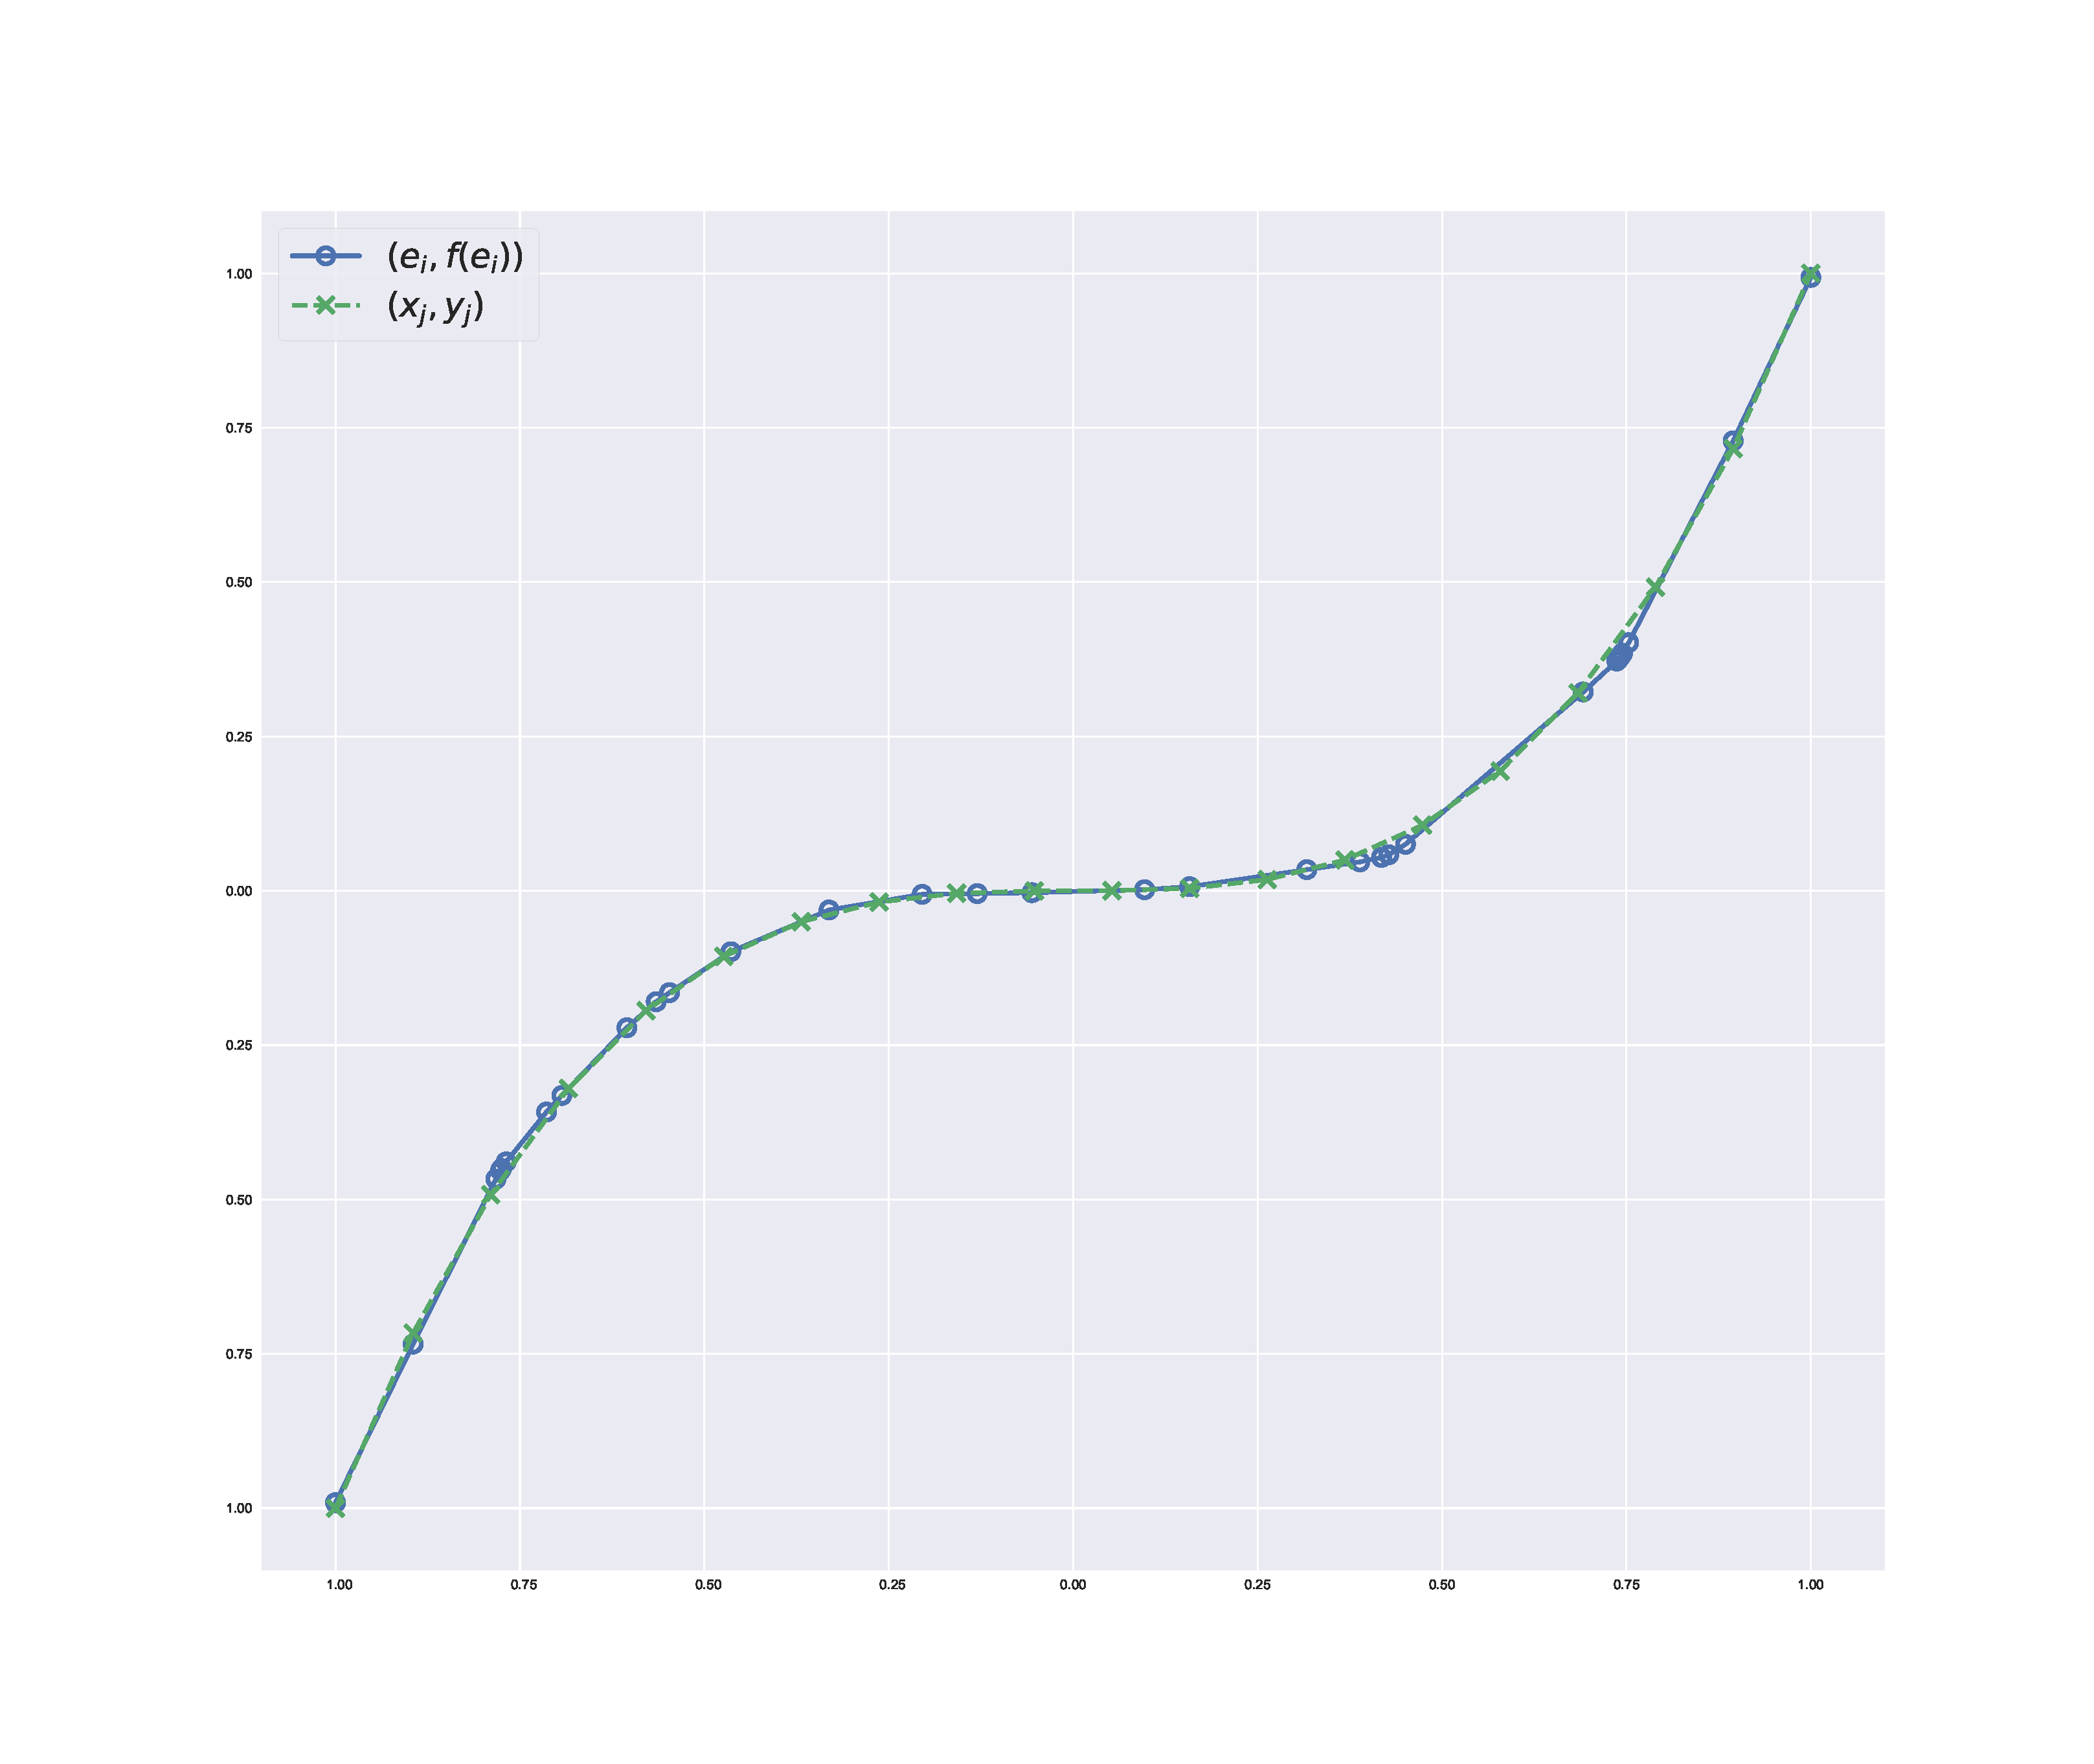
\includegraphics[width=\textwidth]{figures/knots2.pdf}
    \endminipage\hfill
    \minipage{0.5\textwidth}
    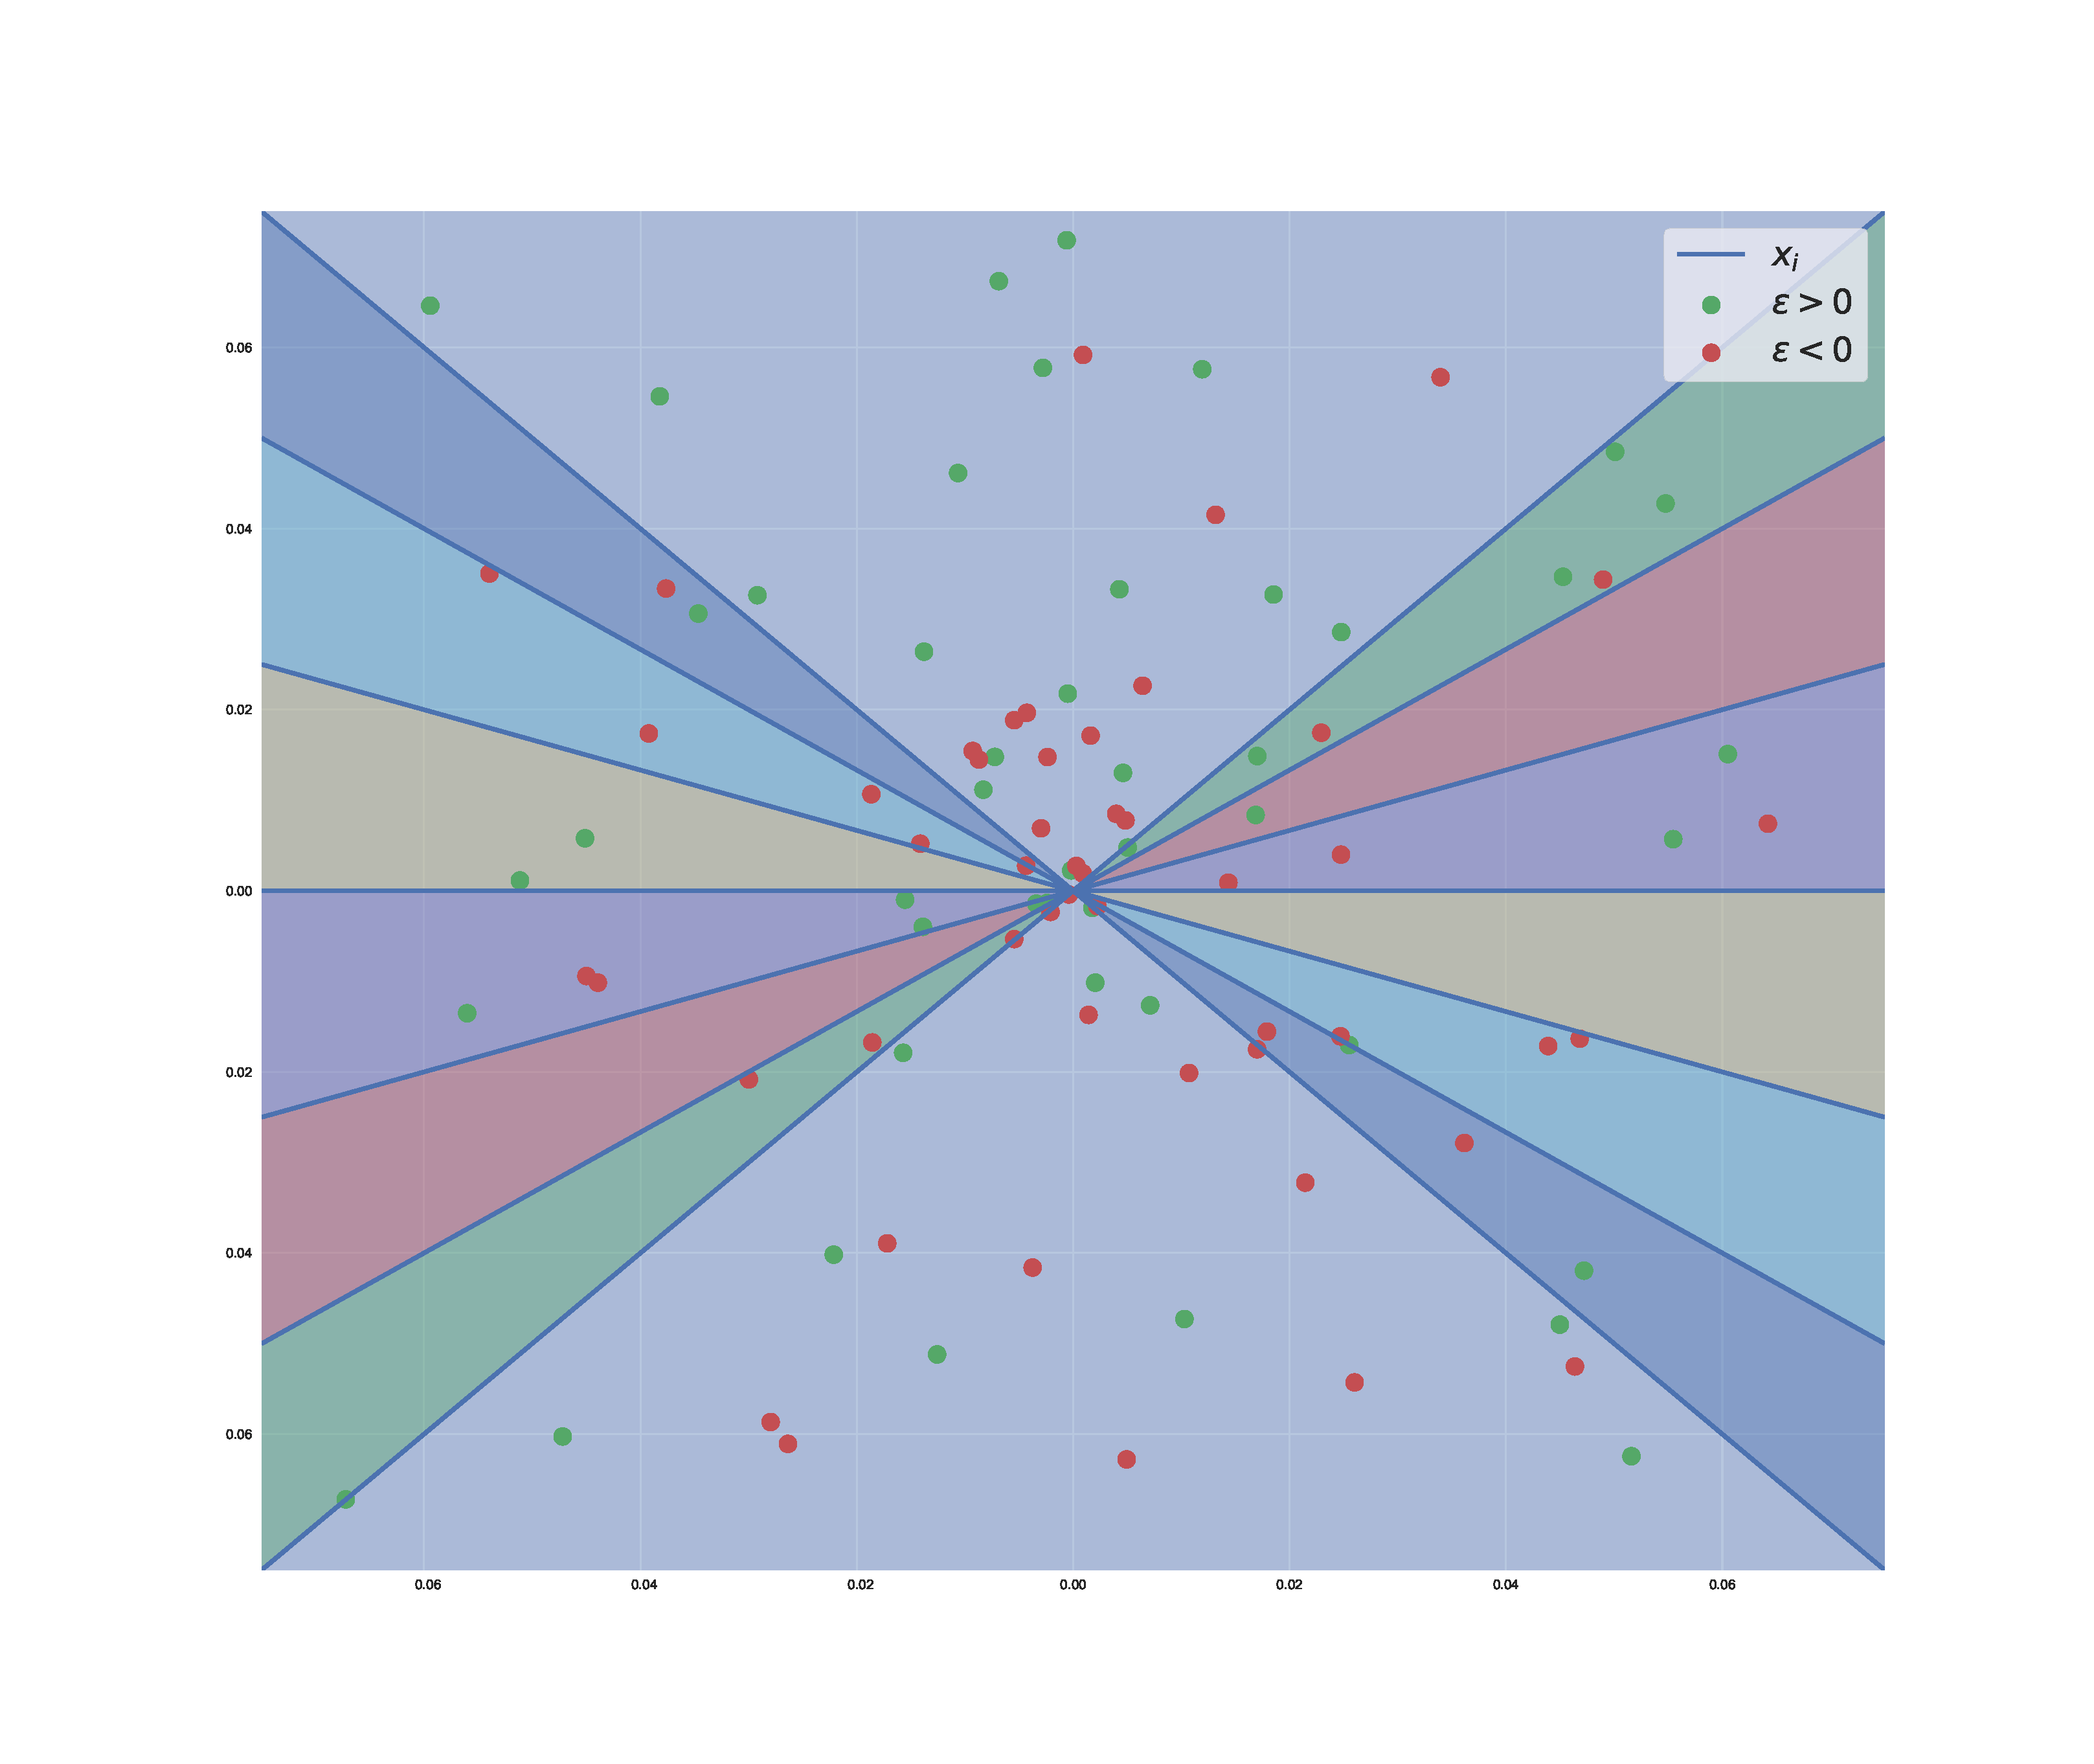
\includegraphics[width=\textwidth]{figures/phaseplot_eg.pdf}
    \endminipage\hfill
    
    
    \caption{\textit{Left:} input samples $(x, y) = (x_j, y_j)_{j=1}^s$ (blue x's) to which we fit a neural network $f_{\bm \xi}(x)$ using the least squares loss \eqref{eq:leastsquares}. $f_{\bm \xi}(x)$ is piecewise linear with the boundaries between pieces occurring at $(e_i, f_{\bm \xi}(e_i))_{i=1}^m$ (green circles). These points correspond to when the operand to one of the ReLUs in \eqref{eq:leastsquares} goes from positive to negative or vice-versa. \textit{Right:} the neurons $\xi_i = (\epsilon_i, u_i, v_i)$ plotted in $u-v$ space. The color of each neuron indicates the sign of $\epsilon_i$. Oberser that the samples $x_j$ correspond to the lines $u x_j + v = 0$ in this space. These sample lines divide the space into the colored regions which correspond to different activation patterns.}
    \label{fig:knots}
\end{figure}


\subsection{Gradient flow}

Our goal is to solve \eqref{eq:leastsquares} using the \emph{gradient flow} (the continuous-time limit of gradient descent) of the least squares loss:

\begin{equation}\label{eq:gradient_flow}
    \bm \xi(0) = \bm \xi_0, \qquad \bm \xi'(t) \in \partial L(\bm \xi(t)).
\end{equation}

Here $\partial L(\bm \xi)$ denotes the \emph{Clarke subdifferential}~\cite{clarke1975generalized}, since $L(\bm \xi)$ is only piecewise smooth. At generic smooth points $\bm \xi$, the subdifferential coincides with the gradient $\partial L(\bm \xi(t)) = \{\nabla L(\bm \xi)\}$. However, we argue in \todo{Section~\ref{todo}} that the discontinuities of the gradient play an important role in the dynamics in practice. For this reason, we subdivide the parameter space into \emph{regions} associated with different \emph{activation patterns} (Figure \ref{fig:knots})

\begin{equation}
    R(\bm \tau, \phi) = \{ (\epsilon, u, v) \, | \, \mathds 1 [u_j x_i + v_j \geq 0] = \tau_{ij}, \, \epsilon = \phi \}
\end{equation}
% \begin{equation}
%     R(\bm \tau,) = \{\bm \xi = (\bm \epsilon, \bm u, \bm v) \in \{-1, 0, 1\} \times \RR^{2m} \, | \, \mathds 1 \rangle (x_i, 1), (u_j, v_j) \rangle  = \tau_{ij},\, {\rm sign}(c_j) = \epsilon_j\}, \quad \bm \tau \in \{0,1\}^{s \times m}, \bm \epsilon \in \{-1,1\}^{m}.
% \end{equation}

If $R(\bm \tau, \phi)$ is not empty, it is a polyhedral cone containing the origin, and it is a product of ``sectors'' corresponding to the activation pattern of each neuron. It is important to note that, in our one-dimensional setting, every neuron can have \emph{at most} $2s$ activation patterns (out of the possible $2^s$ combinatorial types), which means that, for $R(\bm \tau, \phi)$ to be non-empty, the columns of $\bm \tau$ must be chosen among $2s$ possible vectors.
In the interior of a non-empty region $R(\bm \tau, \phi)$, the gradient of $L(\bm \xi)$ can be written as
\begin{equation}\label{eq:derivative_equations}
\begin{gathered}
\nabla L(\bm \xi)_i = \begin{bmatrix}\partial_{u_i} \\ \partial_{v_i}\end{bmatrix} = \epsilon_i \sum_{j=1}^s \tau_{ij} r_j \begin{bmatrix} x_j \\ 1\end{bmatrix}\\
\end{gathered}
\end{equation}
where $r_j = f_{\bm \theta}(x_j) - y_j$ is the $j$-th \emph{residual}. We note that the gradient $\nabla L(\bm \xi)$ is piecewise constant (see Figure~\ref{fig:reduced_grad}) with the discontinuities occurring at the boundaries between regions $R(\bm \tau, \phi)$. The signs $\bm \epsilon$ evolve during the gradient flow as follows:

\begin{equation}
    \epsilon(t) = \text{sign}(
\end{equation}

Finally, we remark that a solution $\bm \xi(t)$ to~\eqref{eq:gradient_flow} will in general converge to a first-order stationary point $\bm \theta^*$ where $0 \in \partial L(\bm \theta^*)$. For certain asymptotic (highly over-parameterized) regimes, it is possible to show convergence to global optima~\cite{du2018gradient,chizat2018global}. In our concrete low dimensional setting, we can state the following result.

\begin{proposition} Let $\bm \xi^* = (\bm \epsilon^*, \bm u^*, \bm v^*)$ be a critical point for $L(\bm \xi)$, and consider the matrix
\begin{equation}
    \bm M_{\bm u^* \bm v^*} = \big [ \langle (x_i, 1), (u_j^*, v_j^*) \rangle_+ \big ]_{ij} \in \RR^{s \times m}.
\end{equation}
If $\bm M_{\bm a^* \bm b^*}$ has full rank, then $L(\bm \theta^*) = 0$, so $\bm \theta^*$ is a global minimum. If $s< m$ and $e_1 \le \ldots \le e_m$ are the knots~\eqref{eq:knots} associated with $\bm \theta^*$, then a sufficient condition for $\bm M_{\bm a^* \bm b^*}$ to have full rank is that each interval $[-\infty, e_1],[e_1,e_2],\ldots,[e_m,\infty]$ contains at most one sample point $x_i$.
\end{proposition}





\subsection{Visualization of reduced parameters}


In the next section, we will illustrate our results by visualizing neurons as in Figure~\ref{fig:phaseplot_eg}. Here, every colored ``particle'' represents a single neuron of $f_{\bm \theta}$ using \emph{reduced coordinates} $\bm \xi$:
\begin{equation}\label{eq:reduced_params}
\bm \xi_i = (u_i,v_i) = (|c_i|a_i,|c_i| b_i), \qquad i=1,\ldots,m.
\end{equation}
The color of the particle indicates the sign $\epsilon_i \in \{+1,-1\}$ of $c_i$ (assuming it is non-zero). Each data point $x_i$ corresponds to a \emph{line} through the origin, namely $u x_i + v =0$. The $2s$ colored sectors indicate regions where neurons have a fixed activation patterns.

Note that although the reduced coordinates $(u_i,v_i)$ do not uniquely identify the parameters $(a_i,b_i,c_i)$, together with $\epsilon_i$ they determine the neuron as a \emph{function}, since $c_i[a_i x + b_i]_+ = \epsilon_i[u_i x + v_i]_+$.
Thus, the reduced parameters determine $f_{\bm \theta}$, but have $m$ fewer degrees of freedom (one per neuron) compared to $\bm \theta$. These degrees of freedom are indeed unnecessary because the association $\bm \theta \rightarrow f_{\bm \theta}$ is not injective. 

% On the other hand, we will argue in the next section that the knowledge of the initial parameters $\bm \theta(0)$ is sufficient recover  to ``lift'' a reduced representation and recover the true neurons.



\section{Training Dynamics}

In this section, we study the trajectories $\bm \theta(t)$ that are solutions of the gradient flow~\eqref{eq:gradient_flow}. As noted in~\cite{NTKJacot}, given a trajectory $\bm \theta(t)$, we can decribe the corresponding path in functional space $f_{\bm \theta(t)}$ using the \emph{tangent kernel} (at least when $\bm \theta$ is in the interior of some activation region $R(\bm \tau,\bm \epsilon)$). In our setting, we consider the map $\Psi: \bm \theta \mapsto {\bm {\hat y}} = (f_{\bm \theta}(x_1),\ldots,f_{\bm \theta}(x_s))$, and have that
\begin{equation}\label{eq:tangent_kernel}
\begin{aligned}
    {\bm {\hat y}}'(t) &= J \Psi(\bm \theta(t)) \cdot J \Psi(\bm \theta(t))^T \cdot \bm r(t)\\
    &= [J_{\bm c} \Psi(\bm \theta(t)) \cdot J_{\bm c} \Psi(\bm \theta(t))^T + J_{\bm a} \Psi(\bm \theta(t)) \cdot J_{\bm a} \Psi(\bm \theta(t))^T + J_{\bm b} \Psi(\bm \theta(t)) \cdot J_{\bm b} \Psi(\bm \theta(t))^T] \cdot \bm r(t)\\
    &= (\bm M_{\bm a\bm b} \bm M_{\bm a\bm b}^T + \bm N^{(1)}_{\bm \tau \bm c} {\bm N_{\bm \tau \bm c}^{(1)T}} + \bm N^{(2)}_{\bm \tau \bm c} {\bm N_{\bm \tau \bm c}^{(2)T}}) \cdot \bm r(t)\\
    & = (\bm K^{\bm c} + \bm K^{\bm a\bm b}) \cdot \bm r(t),
\end{aligned}
\end{equation}
where $\bm r(t) = \bm{\hat y}(t) - \bm y(t)$ is the vector of residuals, and
\begin{equation}
    \bm K^{\bm c}= \bm M_{\bm a\bm b} \bm M_{\bm a\bm b}^T, \qquad
    \bm K^{\bm a \bm b} = \bm N^{(1)}_{\bm \tau \bm c} {\bm N_{\bm \tau \bm c}^{(1)T}} + \bm N^{(2)}_{\bm \tau \bm c} {\bm N_{\bm \tau \bm c}^{(2)T}},
\end{equation}
\begin{equation}
    \bm M_{\bm a\bm b} = [\tau_{ij}(a_j x_i + b_j)]_{ij} \in \RR^{s \times m}, \quad \bm N_{\bm \tau \bm c}^{(1)}= [c_j \tau_{ij} x_i]_{ij} \in \RR^{s \times m},
    \quad \bm N_{\bm \tau \bm c}^{(2)} = [c_j \tau_{ij}]_{ij} \in \RR^{s \times m}.
\end{equation}
The symmetric matrices (kernels) $\bm K^{(c)}$ and $\bm K^{(a,b)}$ in~\eqref{eq:tangent_kernel} describe the trajectory of the predictor $\bm {\hat y}$, but are not constant throughout time. As we argue below, $\bm K^{(c)}$ and $\bm K^{(a,b)}$ affect the trajectory in very different ways: if $\bm K^{(c)}$ ``dominates'' in ~\eqref{eq:tangent_kernel}, we are in the regime of \emph{kernel learning}, for which the bottom layer parameters ($\bm a, \bm b$) are roughly fixed; when instead $\bm K^{(a, b)}$ dominates, then the top layer parameter $\bm c$ is roughly fixed, and we are in a regime that we refer to as \emph{purely adaptive learning}.
In the next subsection, we explain how both extreme regimes can occur at any point in function/predictor space, depending on the initialization of the parameters.
\note{We don't really use this, but maybe it's good to make a clear connection with NTK/lazy learning. Maybe we can shorten it though}

\subsection{Dynamics in reduced parameters}

The matrices $\bm K^{\bm c}$ and $\bm K^{\bm ab}$ depend on the value of the parameters $\bm \theta = (\bm a, \bm b, \bm c)$, and it is in fact easy to realize that they are not constant in a \emph{fiber} of the map $\bm \theta \rightarrow f_{\bm \theta}$, \ie, among the set of parameters representing the same function. This means that even if $\bm \theta_0, \bm \theta_0'$ are such that $f_{\bm \theta_0} = f_{\bm \theta_0'}$, the gradient flow~\eqref{eq:gradient_flow} for $\bm \theta(0) = \bm \theta_0$ or $\bm \theta(0) = \bm \theta_0'$ can converge to very different functions (see Figure~\ref{fig:different_funcs_same_init}). Thus we cannot use the initial state directly to categorize the types of trajectories in the fiber. Instead, the following conserved quantity (which depends only on $\bm \theta_0$) categorizes the trajectory of $\bm \theta(t)$:

\begin{lemma} \label{le:fixed_delta}
If $\bm \theta(t) = (\bm a(t), \bm b(t), \bm c(t))$ is a solution of the integral flow \eqref{eq:gradient_flow}, then the quantities
\begin{equation}\label{eq:invariants}
\delta_i = c_i(t)^2 - a_i(t)^2 - b_i(t)^2, \quad i = 1, \ldots, m,
\end{equation}
remain constant for all $t$. In particular, given a reduced representation of a neuron $(u_i,v_i) = (|c_i|a_i,|c_i|b_i)$, we can recover the original neuron $(a_i,b_i,c_i)$ up to the sign of $c_i$, since
\begin{equation}\label{eq:c_uv}
    c_i^2 = \frac{\delta_i + \sqrt{\delta_i^2 + 4 (u_i^2 + v_i^2)}}{2}. 
\end{equation}
\end{lemma}

We next assume that $\bm \theta$ is a parameter in the interior of an activation region $R(\bm \tau, \bm \epsilon)$. We define the \emph{loss in reduced parameters} \note{Notation?}
\begin{equation}
    \tilde L(\bm \xi) = \sum_{i=1}^s |g_{\bm \epsilon, \bm \xi}(x_i) - y_i|^2, \qquad \bm \xi = (\bm u, \bm v) \in \RR^{2m},  
\end{equation}
\begin{equation}
    g_{\bm \epsilon,\bm \xi}(x) = \sum_{j=1}^m \epsilon_i [ u_i x + v_i]_+.
\end{equation}
Inside $R(\bm \tau,\bm \epsilon)$ (where the sign vector $\bm \epsilon$ is fixed) the gradient of the loss in reduced parameters $\nabla \tilde L(\bm \xi)$ is very simple: indeed, the association $\bm \xi \rightarrow (g_{\bm \xi}(x_1),\ldots,g_{\bm \xi}(x_s))$ is \emph{linear}, since $g_{\bm \xi}(x_i) = \sum_{i=1}^m \tau_{ij} \epsilon_j (u_j x_i + v_j)$, so the field $\nabla \tilde L(\bm \xi)$ points in a unique direction (see Figure~\ref{fig:reduced_grad})

\begin{theorem}\label{thm:reduced_parameter_grad}
Let $\bm \theta(t)$ be an integral curve for the gradient flow \eqref{eq:gradient_flow} of $L(\bm \theta)$, and let $\bm \delta = (\delta_i) \in \RR^m$ be the vector of invariants~\eqref{eq:invariants}, which depend only on the initialization $\bm \theta(0)$. If $\bm \xi(t) = (\bm u(t), \bm v(t))$ is curve of reduced parameters corresponding to $\bm \theta(t)$, then we have that
\begin{equation}
\begin{bmatrix}
\dot u_i(t)\\
\dot v_i(t)
\end{bmatrix} =
\bm P_{\delta_i}(u_i,v_i)
\begin{bmatrix}
\nabla_{u_i} \tilde L (\bm \xi)\\
\nabla_{v_i} \tilde L (\bm \xi)\\
\end{bmatrix},
\quad i=1,\ldots,m,
\end{equation}
where
\begin{equation}\label{eq:neuron_kernel}
\bm P_\delta(u_i,v_i) = \begin{bmatrix}
    a_i^2 + c_i^2  & 
    a_i b_i        \\
    a_i b_i               & 
    b_i^2 + c_i^2\\
\end{bmatrix} = 
\begin{bmatrix}
\frac{u_i^2}{c(u_i, v_i)^2} + c(u_i, v_i)^2 & \frac{u_i v_i}{c(u_i, v_i)^2}\\
\frac{u_i v_i}{c(u_i, v_i)^2} &  \frac{v_i^2}{c(u_i, v_i)^2} + c(u_i, v_i)^2\\
\end{bmatrix},
\end{equation}

and $c(u_i, v_i)^2 = \frac{\delta_i + \sqrt{\delta_i^2 + 4 (u_i^2 + v_i^2)}}{2}$
\end{theorem}




% We also explore the special case of \emph{lazy training} (\cite{NTKJacot}, \cite{chizat2018note}) where the parameters of the first layer ($a$ and $b$) are fixed and the parameters of the outer layer ($c$) are allowed to move. We show that in the lazy regime, the solution to gradient descent is a natural cubic spline.


This Theorem shows how the dynamics of a (reduced) neuron are related to the simpler (locally linear) dynamics of the reduced loss. It is easy to verify that the eigenvalue-eigenvector pairs of $\bm P_{\delta_i}(u_i,v_i)$ are
\begin{align}
    (\lambda_1, \bm w_1) &= (a_i^2+ b_i^2 + c_i^2, (u_i,v_i))
    % = \left(\frac{1}{c^2}(\beta(a^2 + b^2) + \alpha), \left(\frac{u}{|c|}, \frac{v}{|c|}\right)\right)
    \label{eq:radial_eigenval}\\
    (\lambda_2, \bm w_2) &= (c_i^2, (-v_i,u_i)) 
    % = \left(\alpha c^2, \left(-\frac{v}{|c|}, \frac{v}{|c|}\right)\right)
    \label{eq:tangential_eigenval}
\end{align}
The eigenvectors of $\bm P_{\delta_i}(u_i,v_i)$ define two extreme trajectories, and we can understand the dynamics of a neuron as a continuum between these extrema. In fact, writing $\rho_i = u_i^2 + v_i^2$, it is straightforward to verify that:

\begin{itemize}
    \item If $\rho_i \ll |\delta_i|$ and $\delta < 0$, then $\xi'(t) \propto \xi$, and the neuron moves \emph{radially}.
    \item If $\rho_i \ll |\delta_i|$ and $\delta > 0$, then $(\dot u_i(t), \dot v_i(t)) \propto \nabla_{u_i} \tilde L(\bm \xi(t))$, so the reduced neuron moves parallel to the vector field $\nabla \tilde L(\bm \xi)$.
\end{itemize}
It is also interesting to note that the trajectories of neurons follow paths that are (up to rotations) solutions to one of two possible ODEs: indeed, we can always assume $\bm \delta_i = \pm 1$ given that
\begin{equation}
\bm P_{\delta_i}(u_i,v_i)\cdot v = \bm P_{\delta_i/|\delta_i|} \left(\frac{u_i}{|\delta_i|},\frac{v_i}{|\delta_i|}\right) \cdot |\delta_i|v.
\end{equation}
This means the trajectory of a neuron can be understood locally by considering the vector field $\bm P_{\pm 1}(u_i,v_i) \cdot \nabla \tilde{L}(\bm \xi)$ at a different (rescaled) point. \note{Show figure of the two vector fields}

\begin{figure}\label{fig:trajectories}
    \centering
    \minipage{0.33\textwidth}
    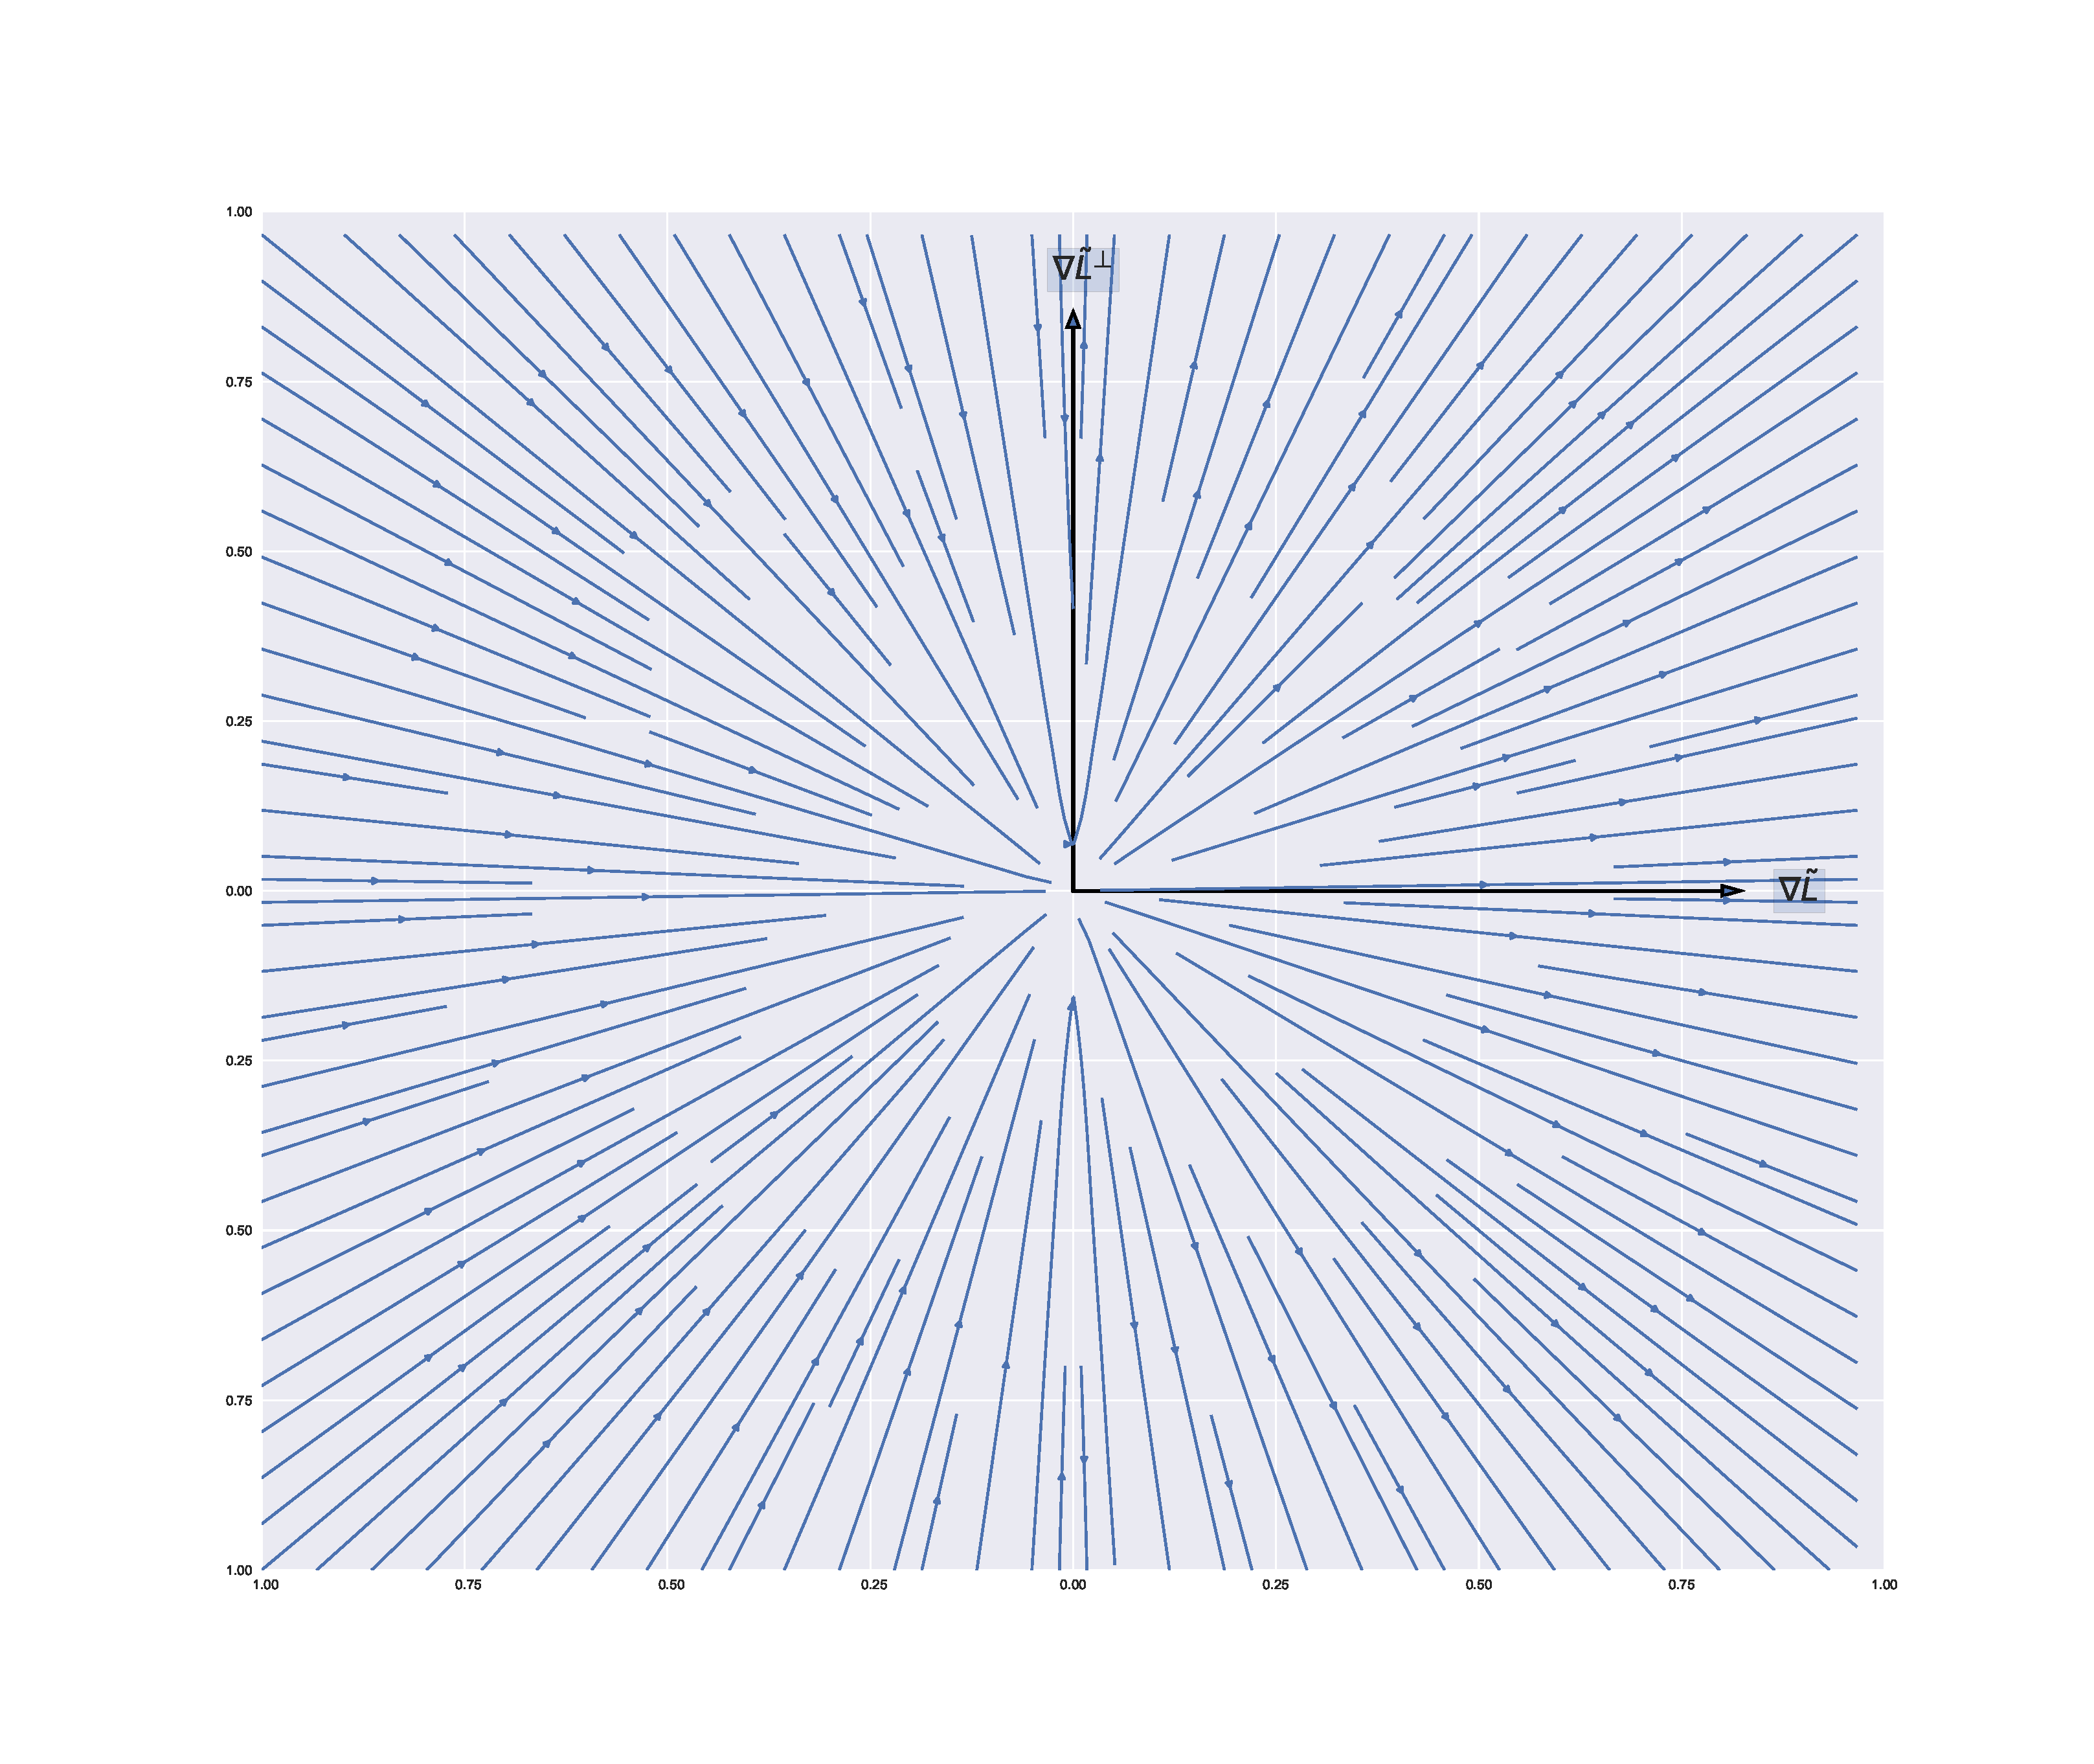
\includegraphics[width=\linewidth]{figures/dynamics_delta_-100.pdf}
    \endminipage\hfill
    % \minipage{0.2\textwidth}
    % 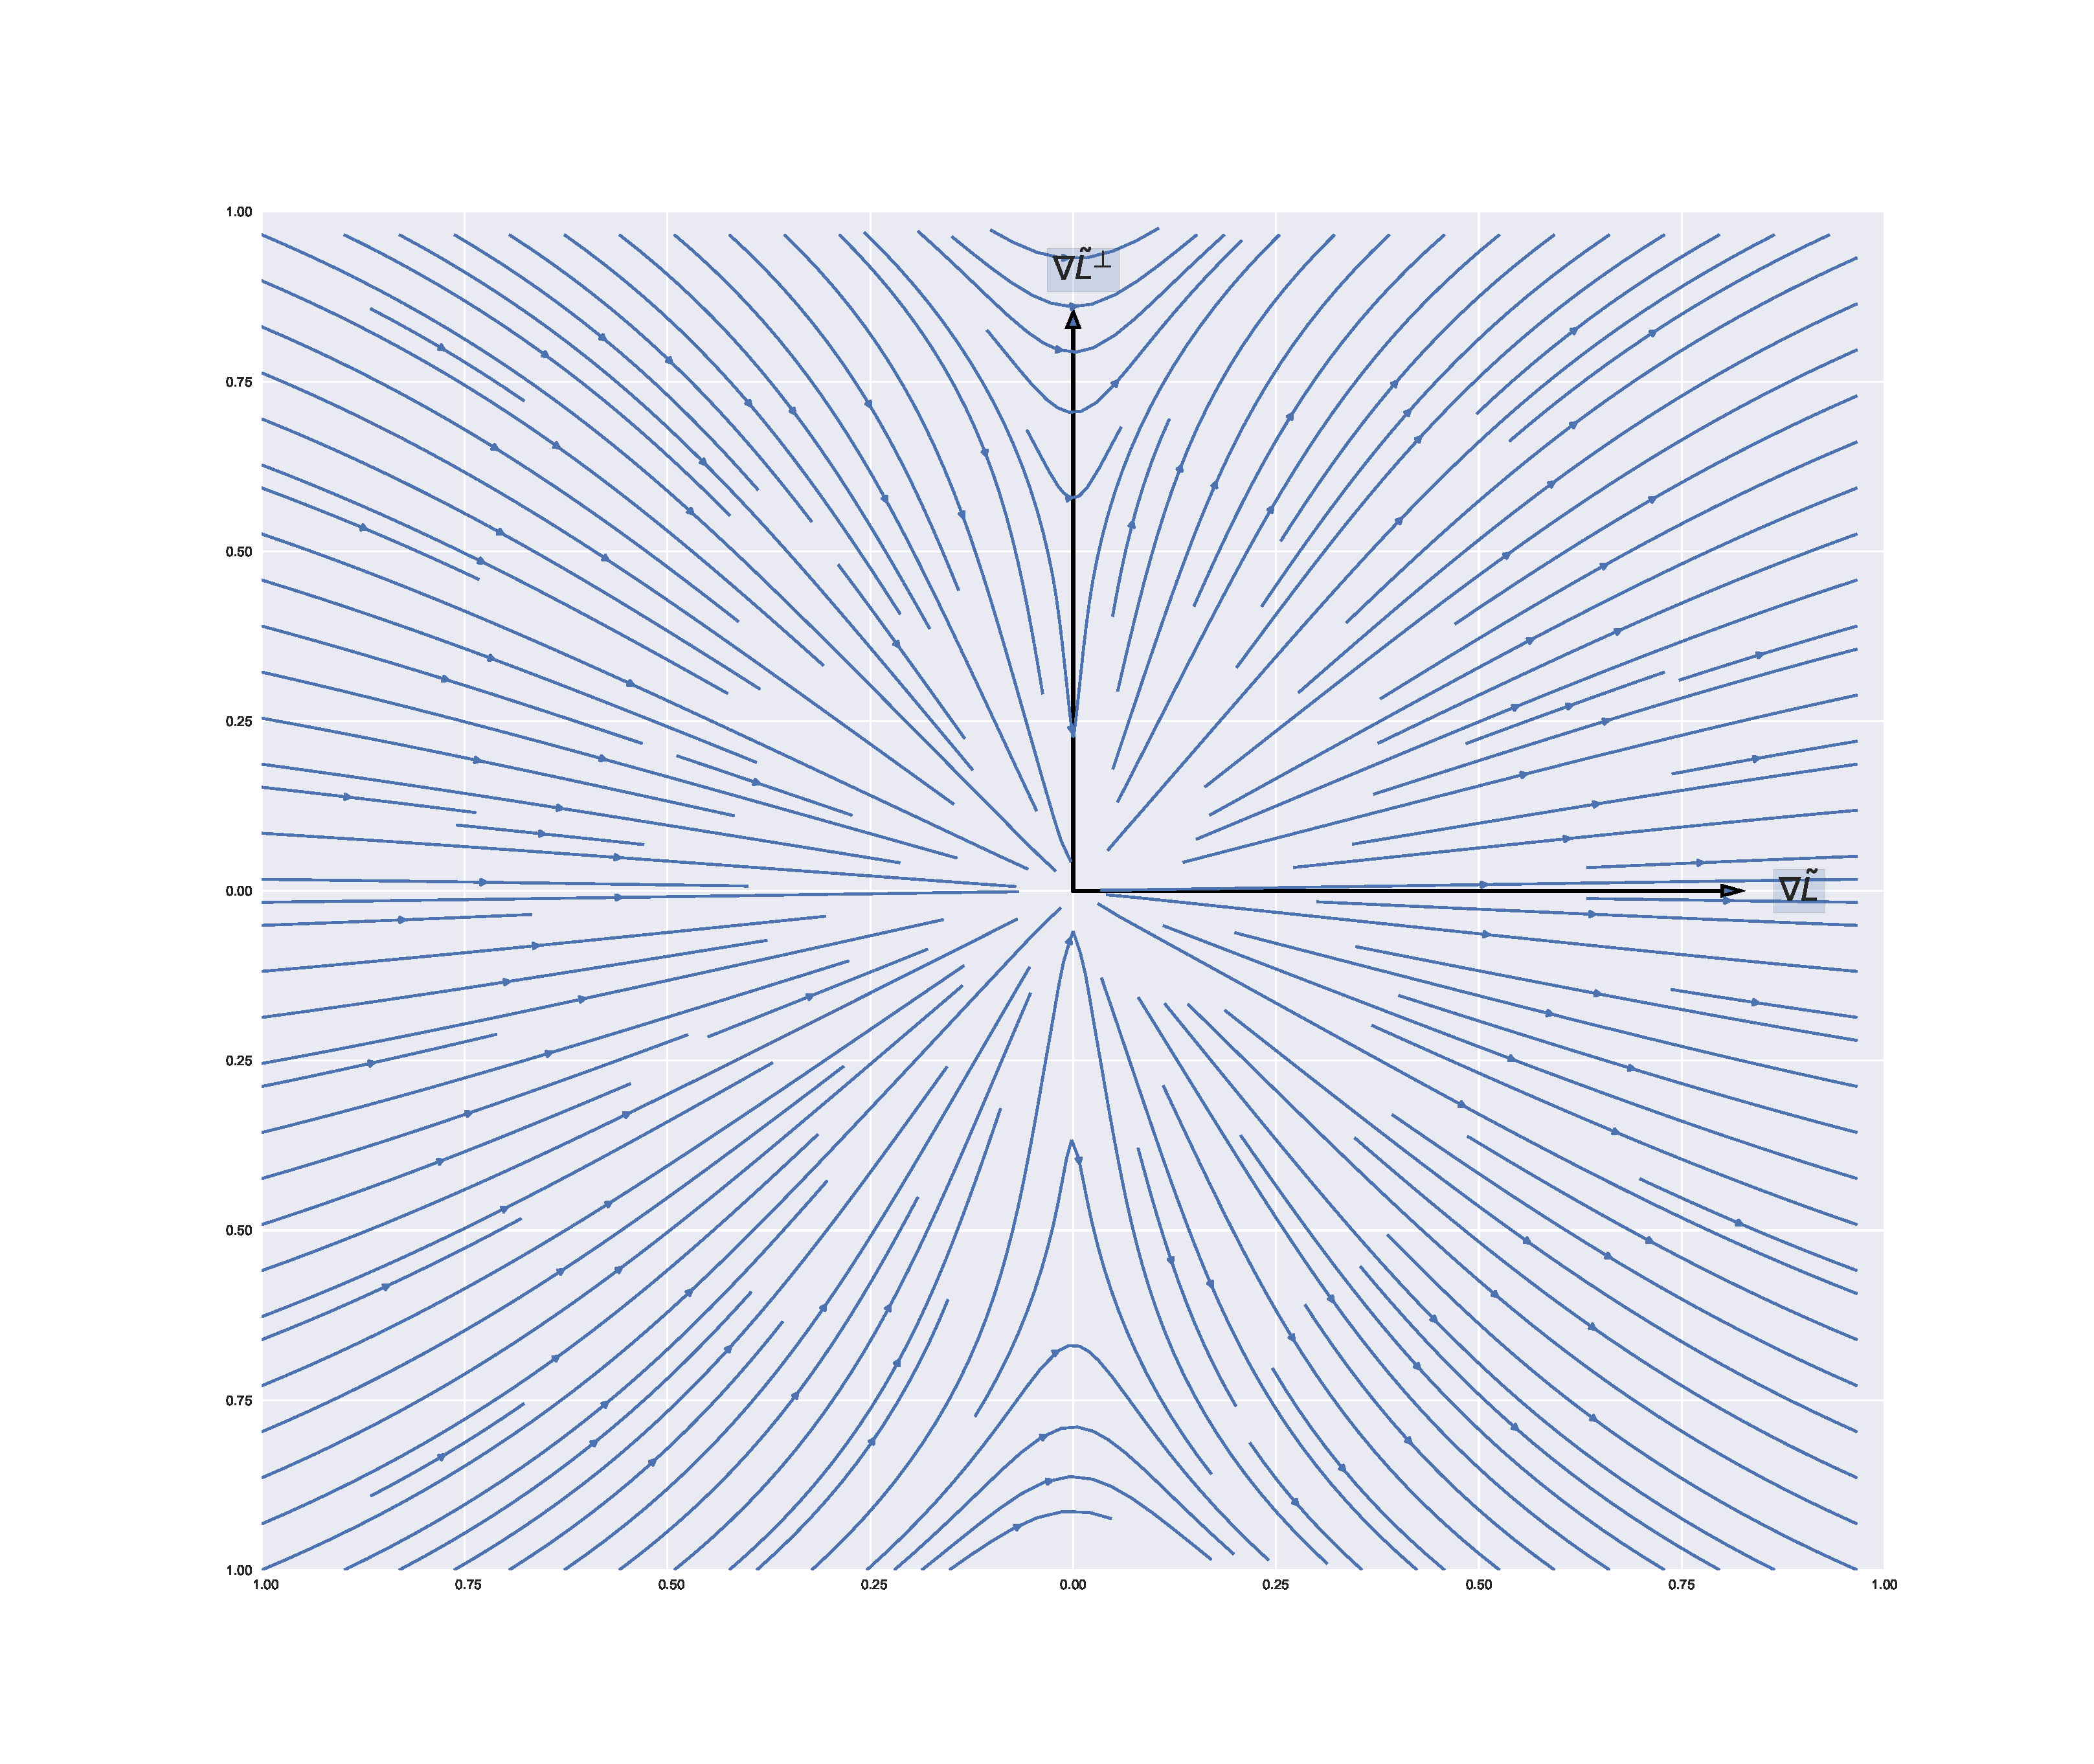
\includegraphics[width=\linewidth]{figures/dynamics_delta_-1.pdf}
    % \endminipage\hfill
    \minipage{0.33\textwidth}
    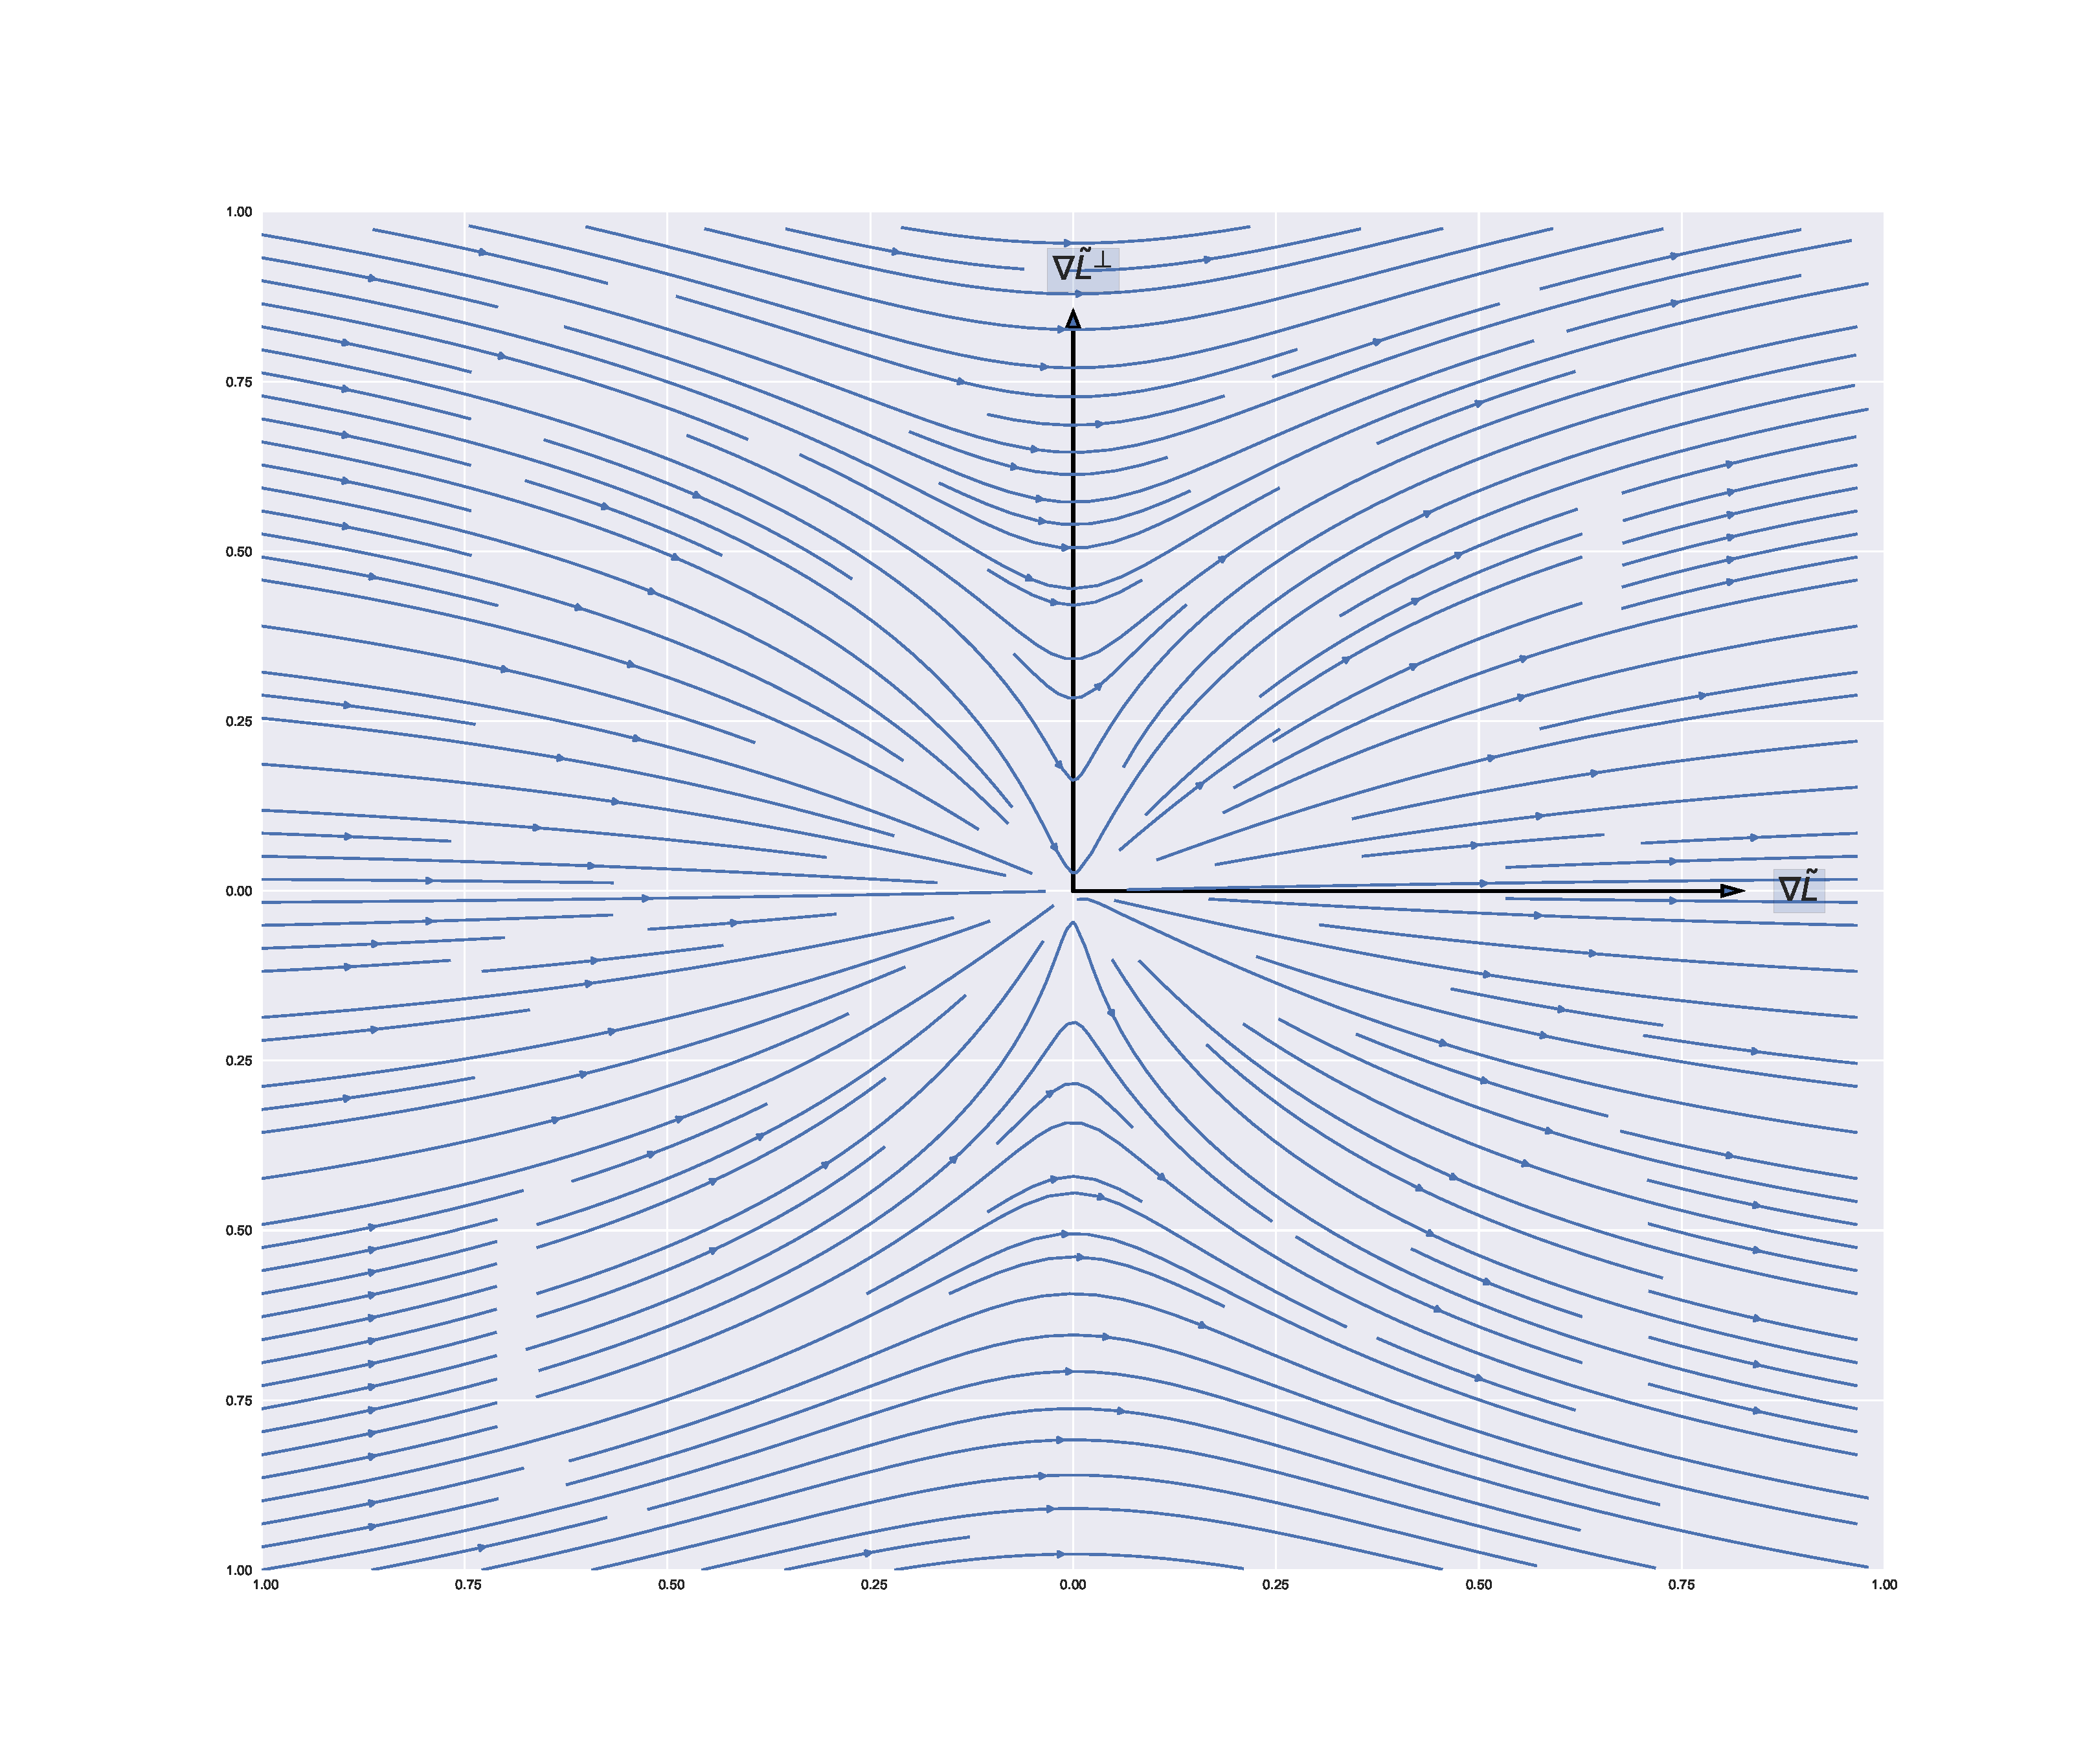
\includegraphics[width=\linewidth]{figures/dynamics_delta_0.pdf}
    \endminipage\hfill
    % \minipage{0.2\textwidth}
    % 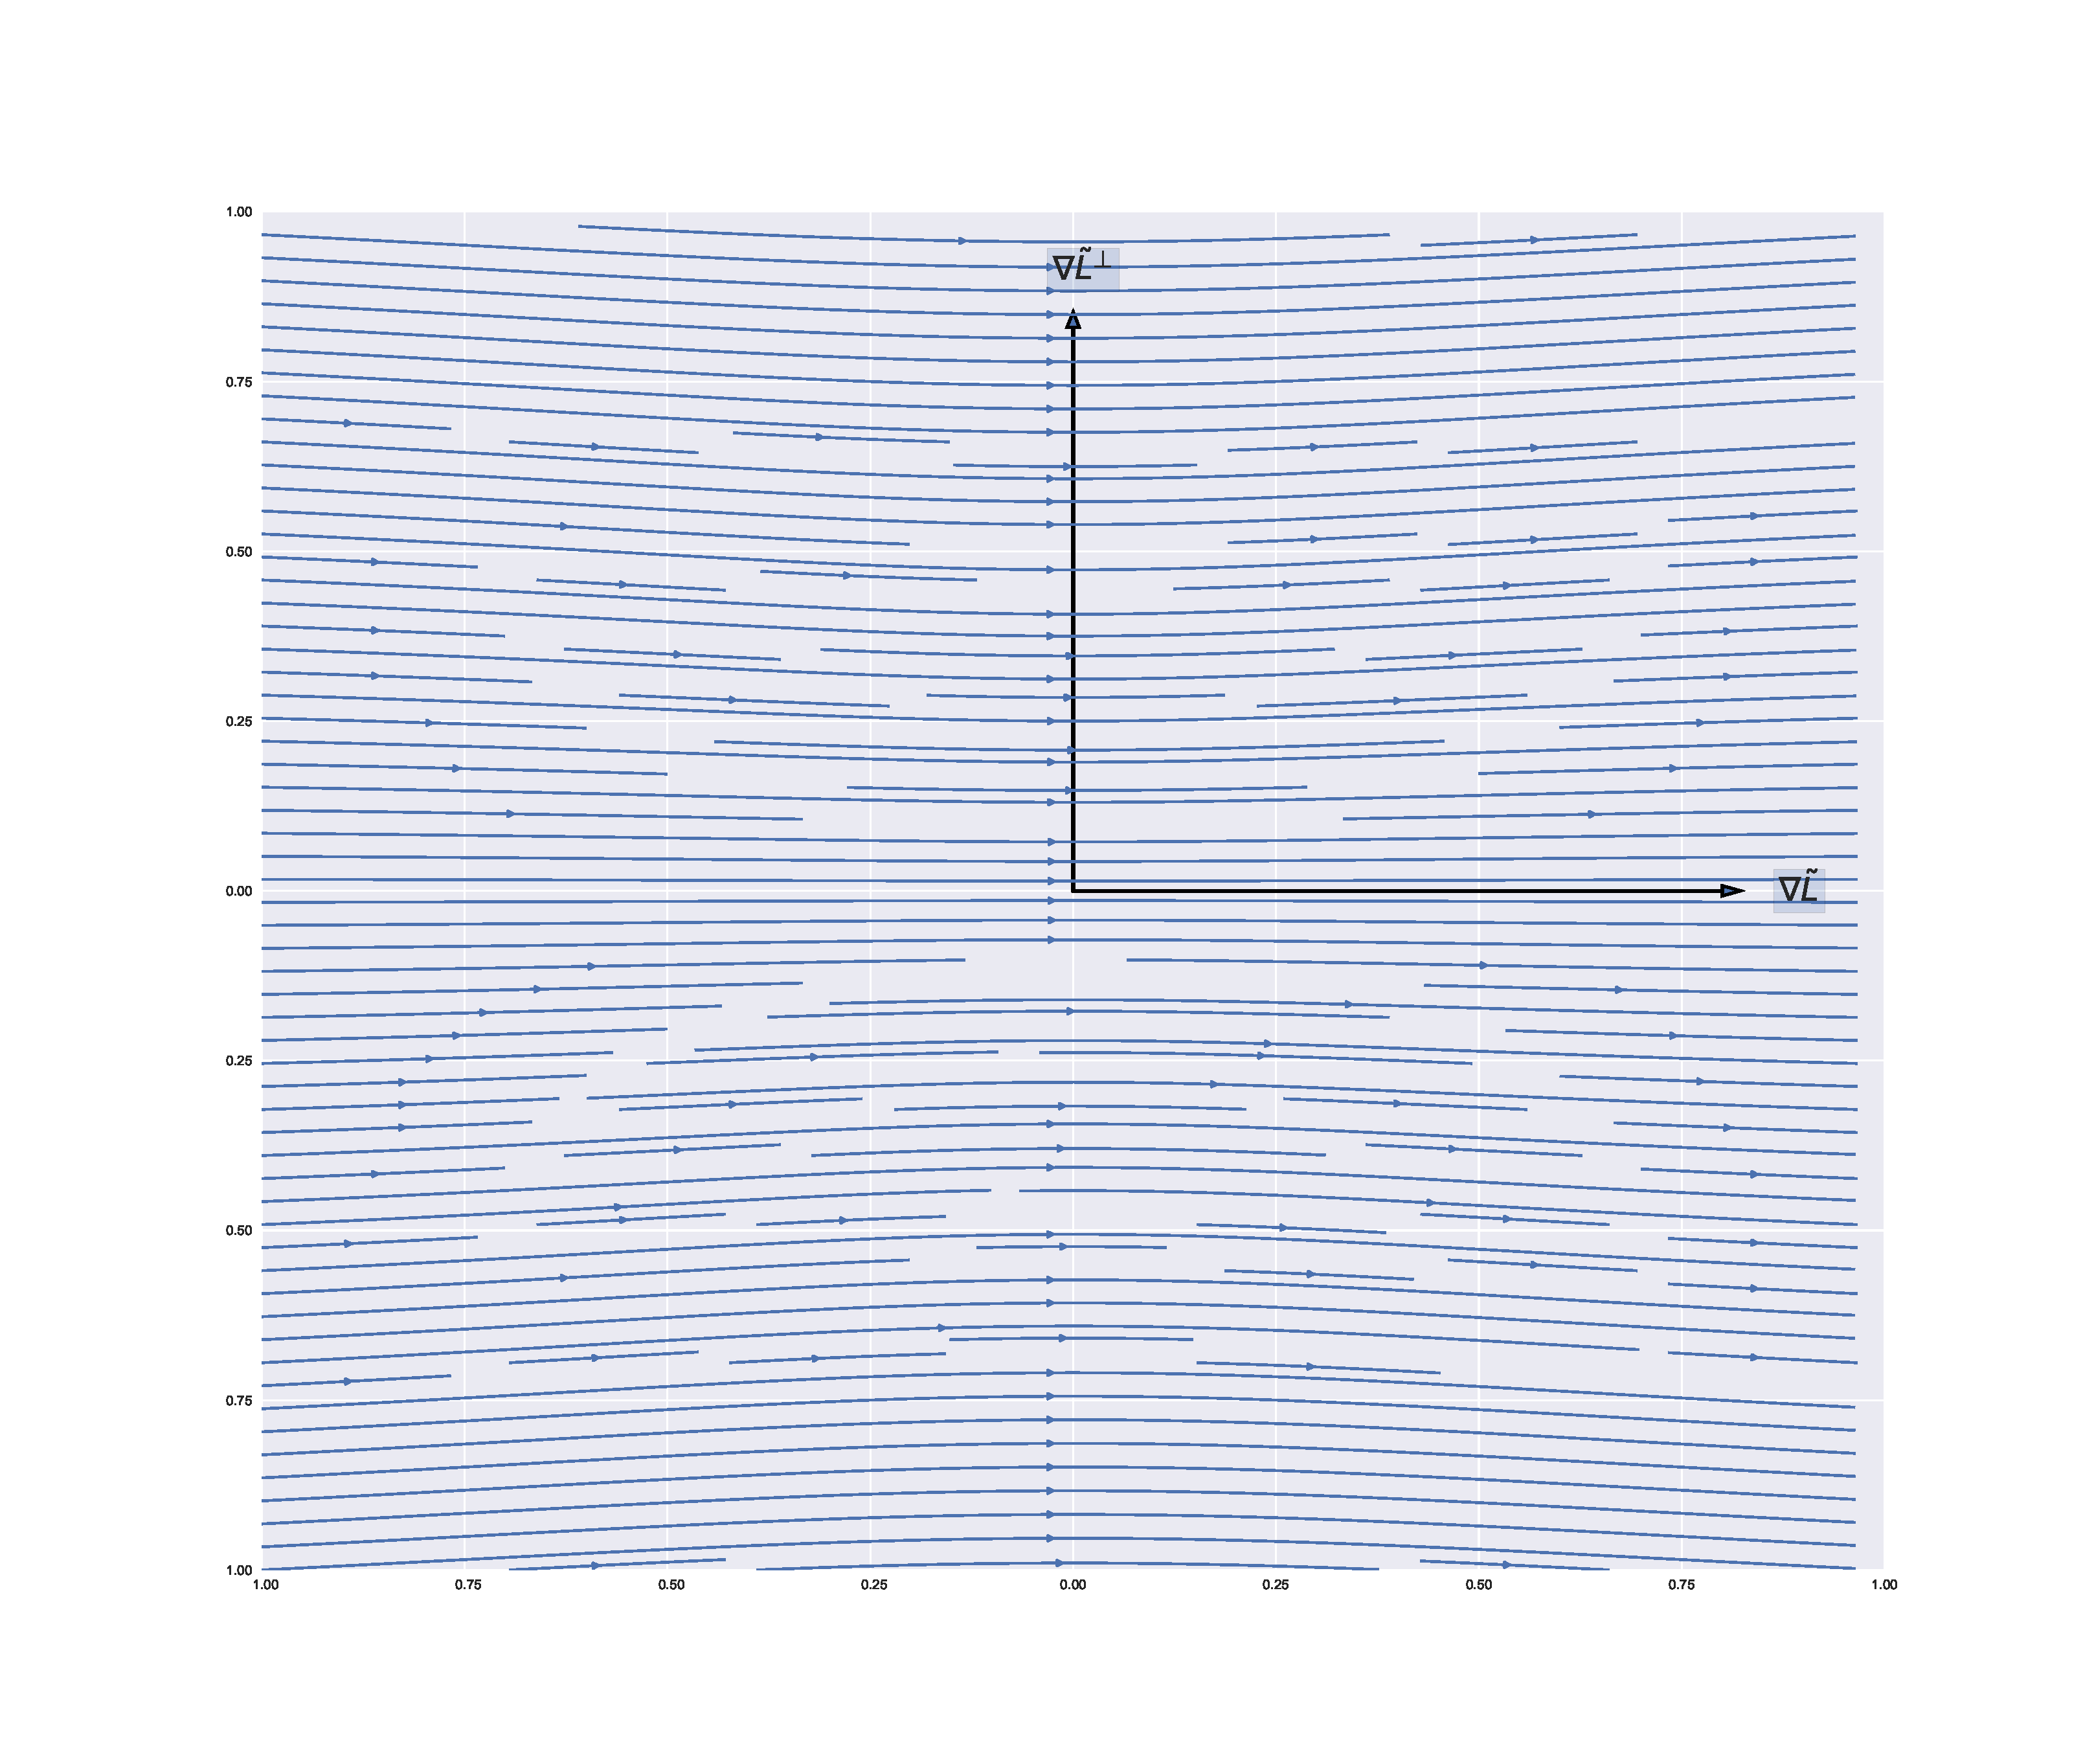
\includegraphics[width=\linewidth]{figures/dynamics_delta_1.pdf}
    % \endminipage\hfill
    \minipage{0.33\textwidth}
    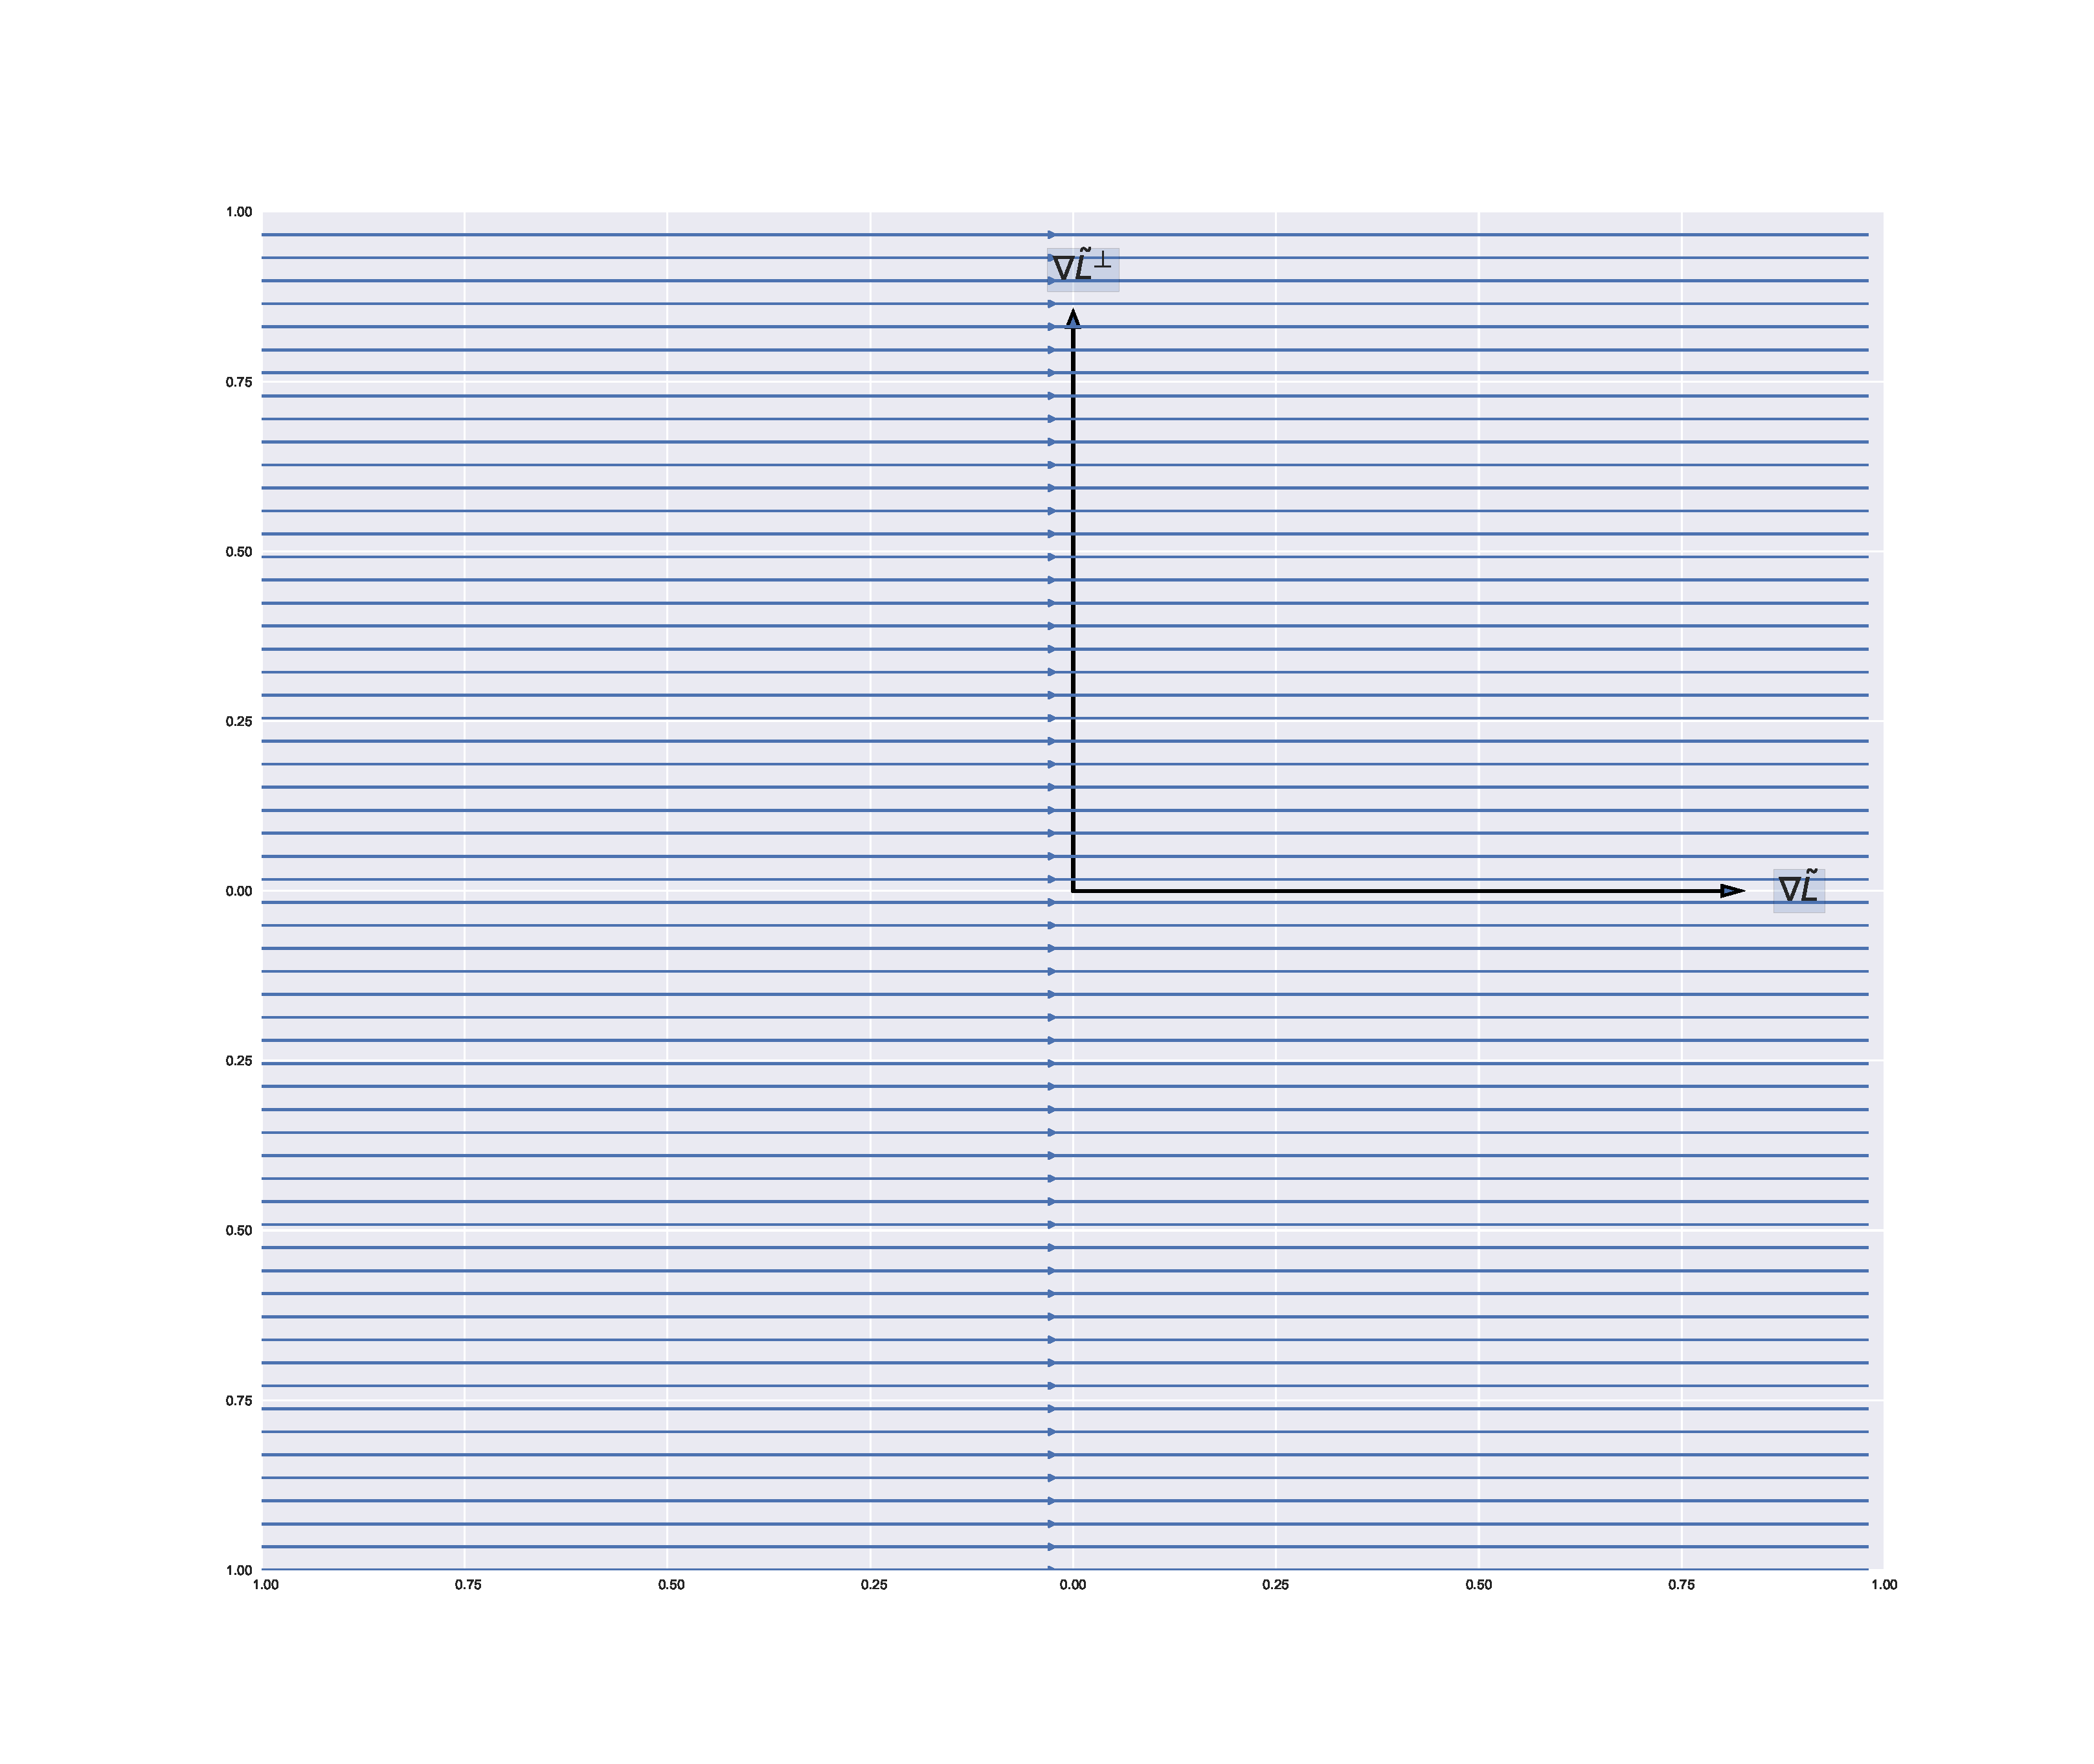
\includegraphics[width=\linewidth]{figures/dynamics_delta_100.pdf}
    \endminipage
    
    \caption{The value of $\delta$ interpolates between different kinds of local trajectories of neurons. The plots are in the coordinate frame $(\nabla \tilde{L}, \nabla \tilde{L}^\bot)$. The left shows $\delta = -100$, in this case, the neurons move radially towards and away from the origin. The middle image shows the trajectories for $\delta = 0$ which has trajectories containing both radial and tangential components. The right image shows the trajectories for $\delta = 100$ which are parallel to the gradient $\nabla \tilde{L}$.}
    \label{fig:my_label}
\end{figure}

\begin{figure}\label{fig:different_funcs_same_init}
    \centering
    \minipage{0.33\textwidth}
    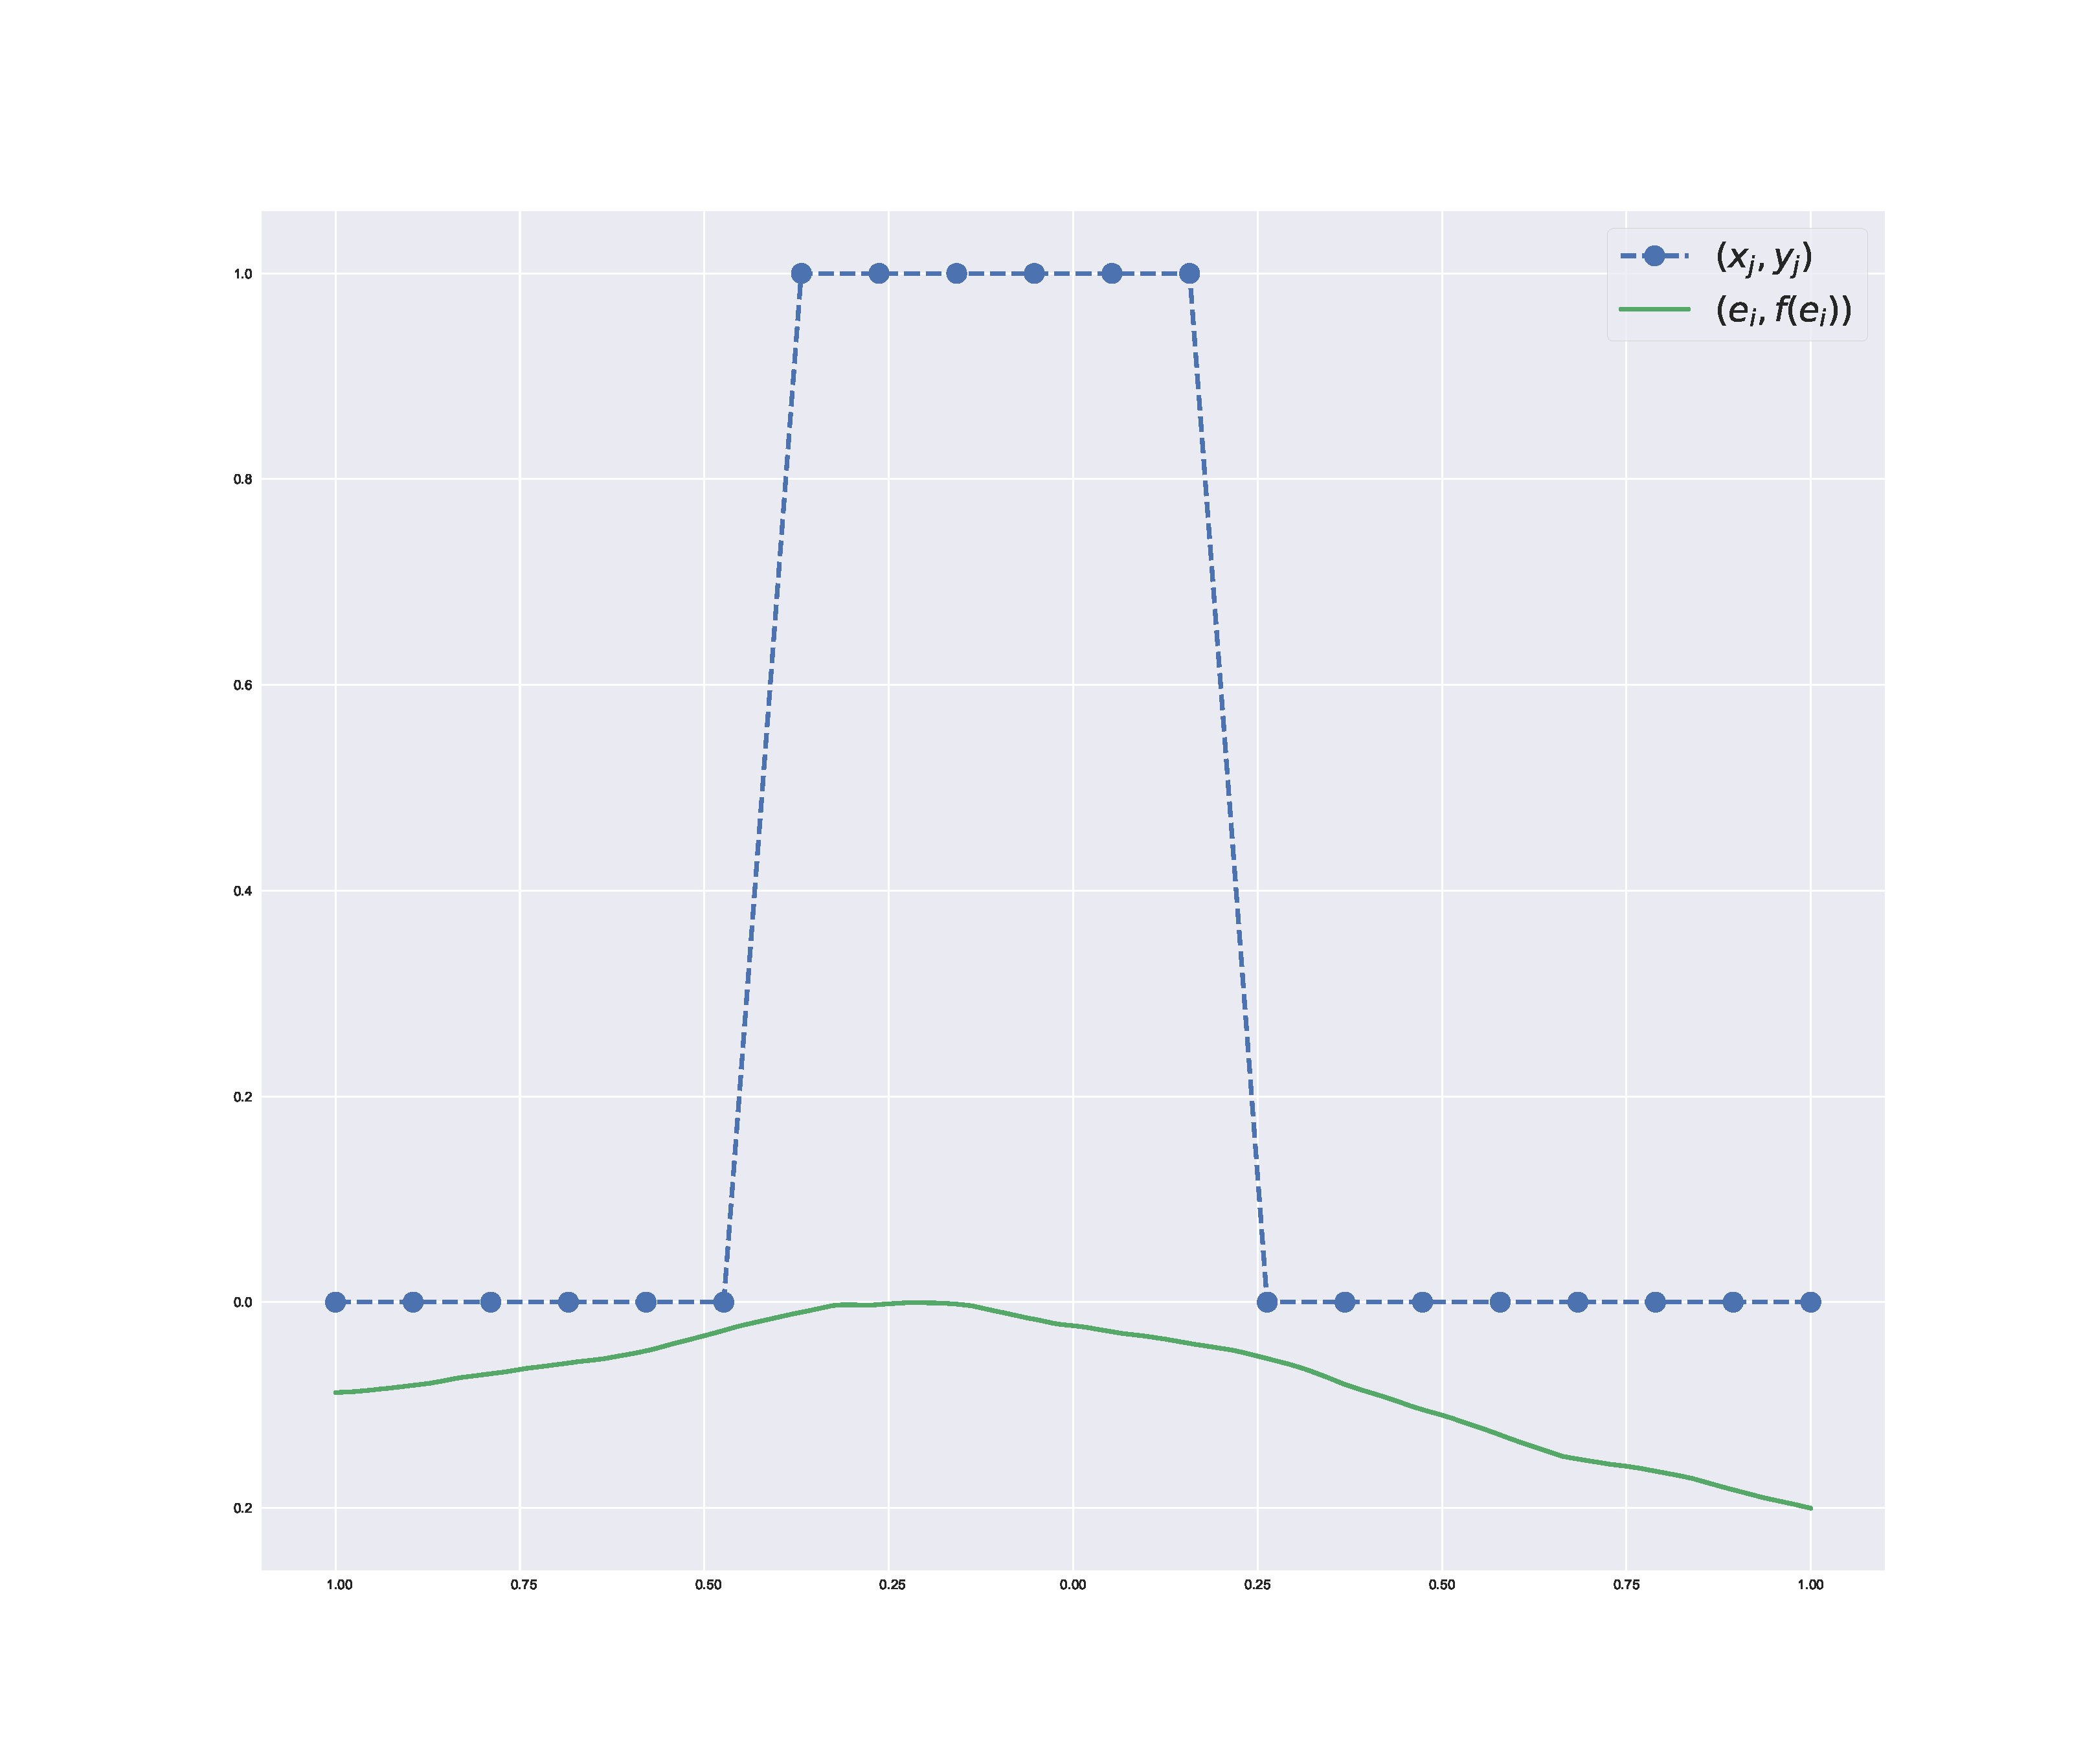
\includegraphics[width=\linewidth]{figures/same_init_different_func_square_init.pdf}
    \endminipage\hfill
    % \minipage{0.2\textwidth}
    % 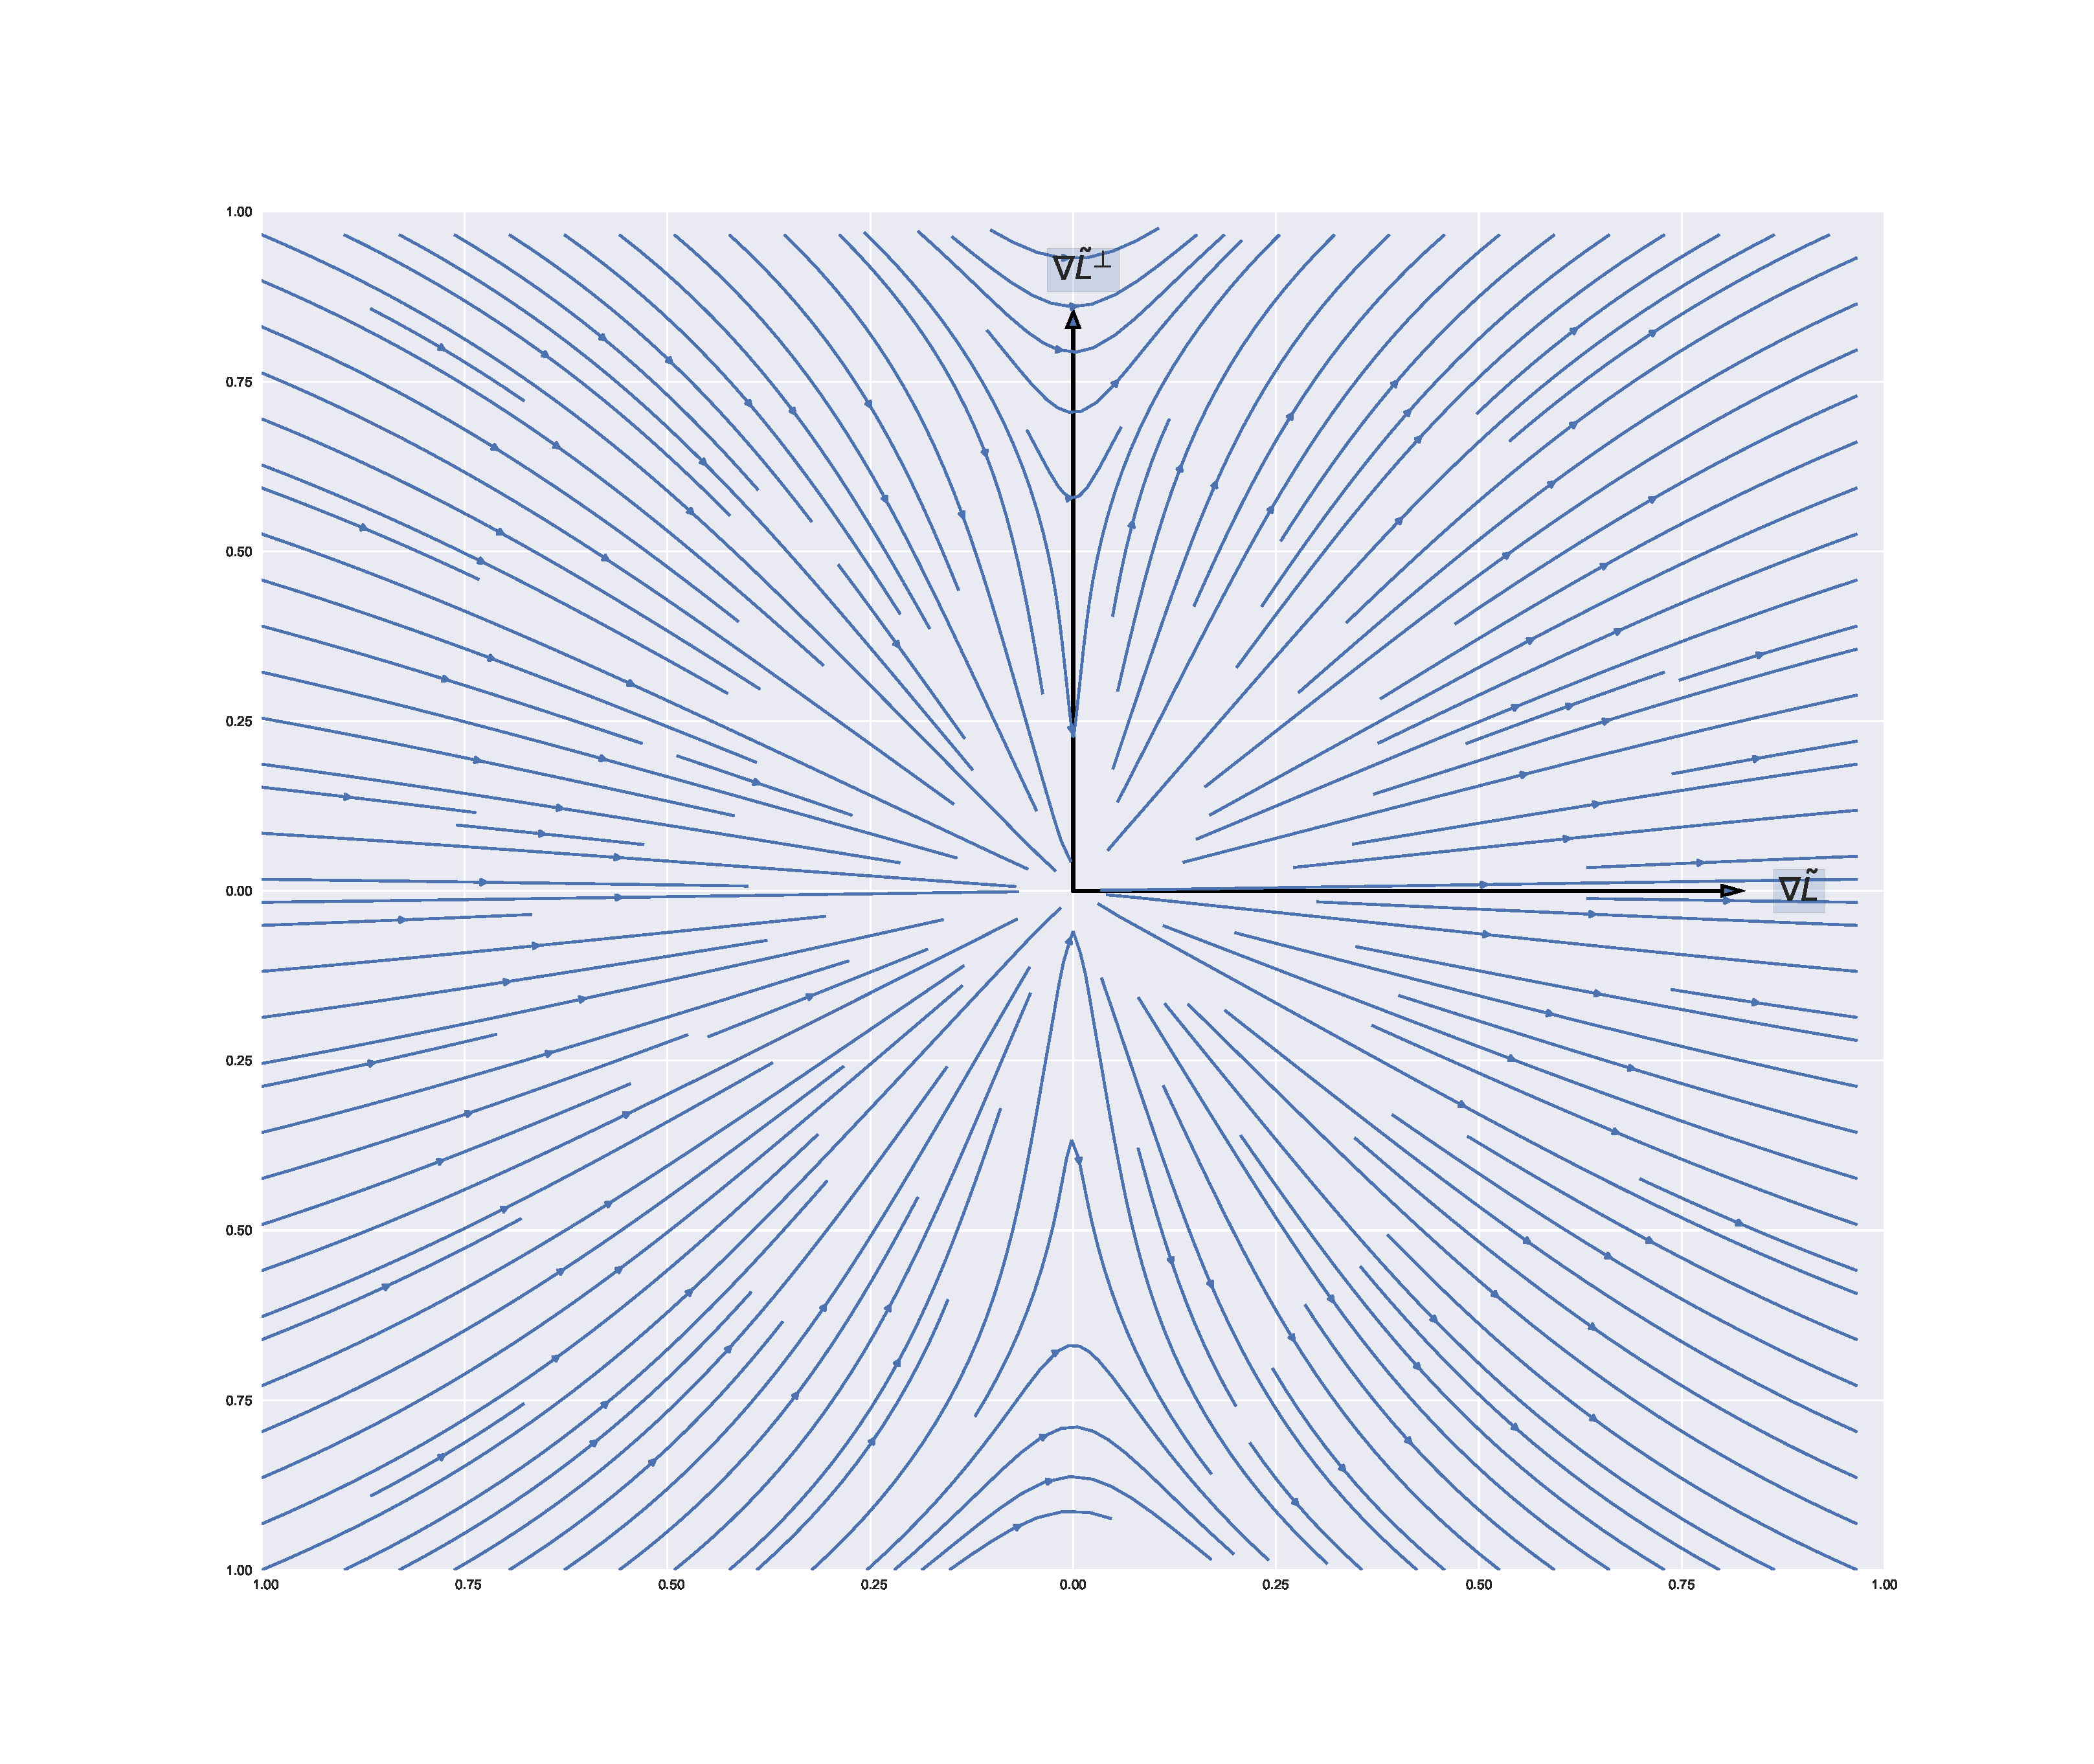
\includegraphics[width=\linewidth]{figures/dynamics_delta_-1.pdf}
    % \endminipage\hfill
    \minipage{0.33\textwidth}
    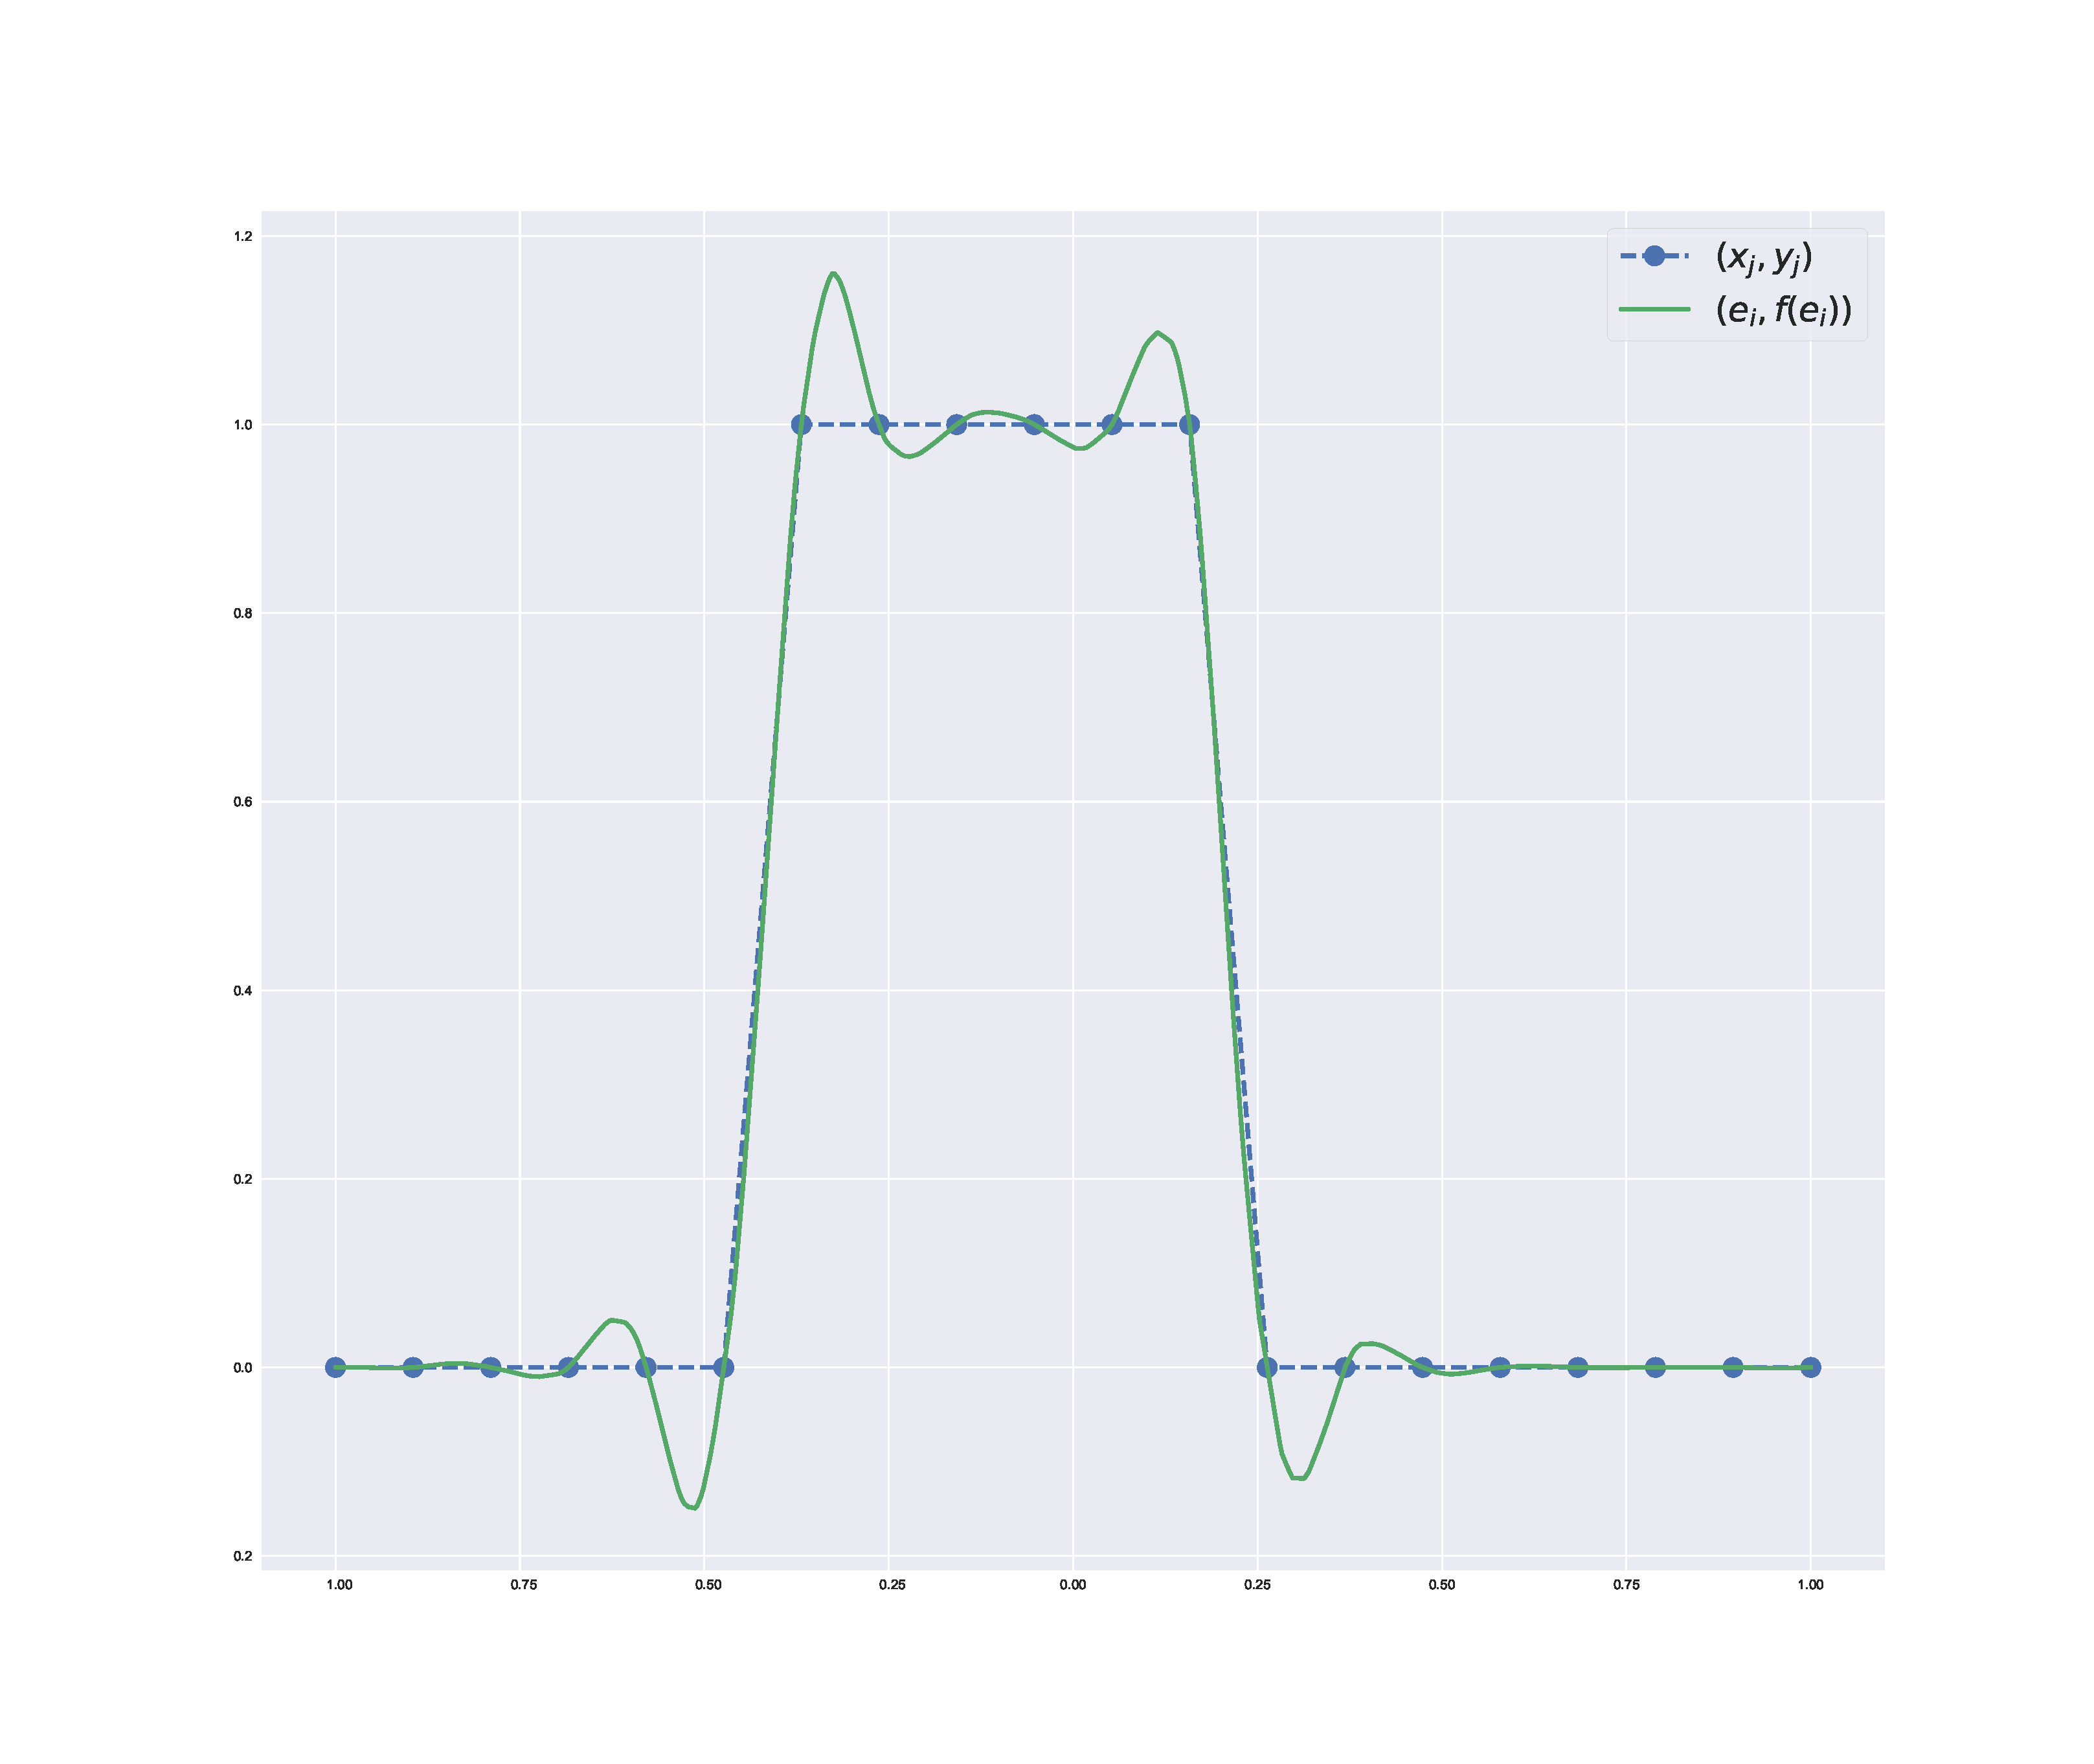
\includegraphics[width=\linewidth]{figures/same_init_different_func_square_1.pdf}
    \endminipage\hfill
    % \minipage{0.2\textwidth}
    % 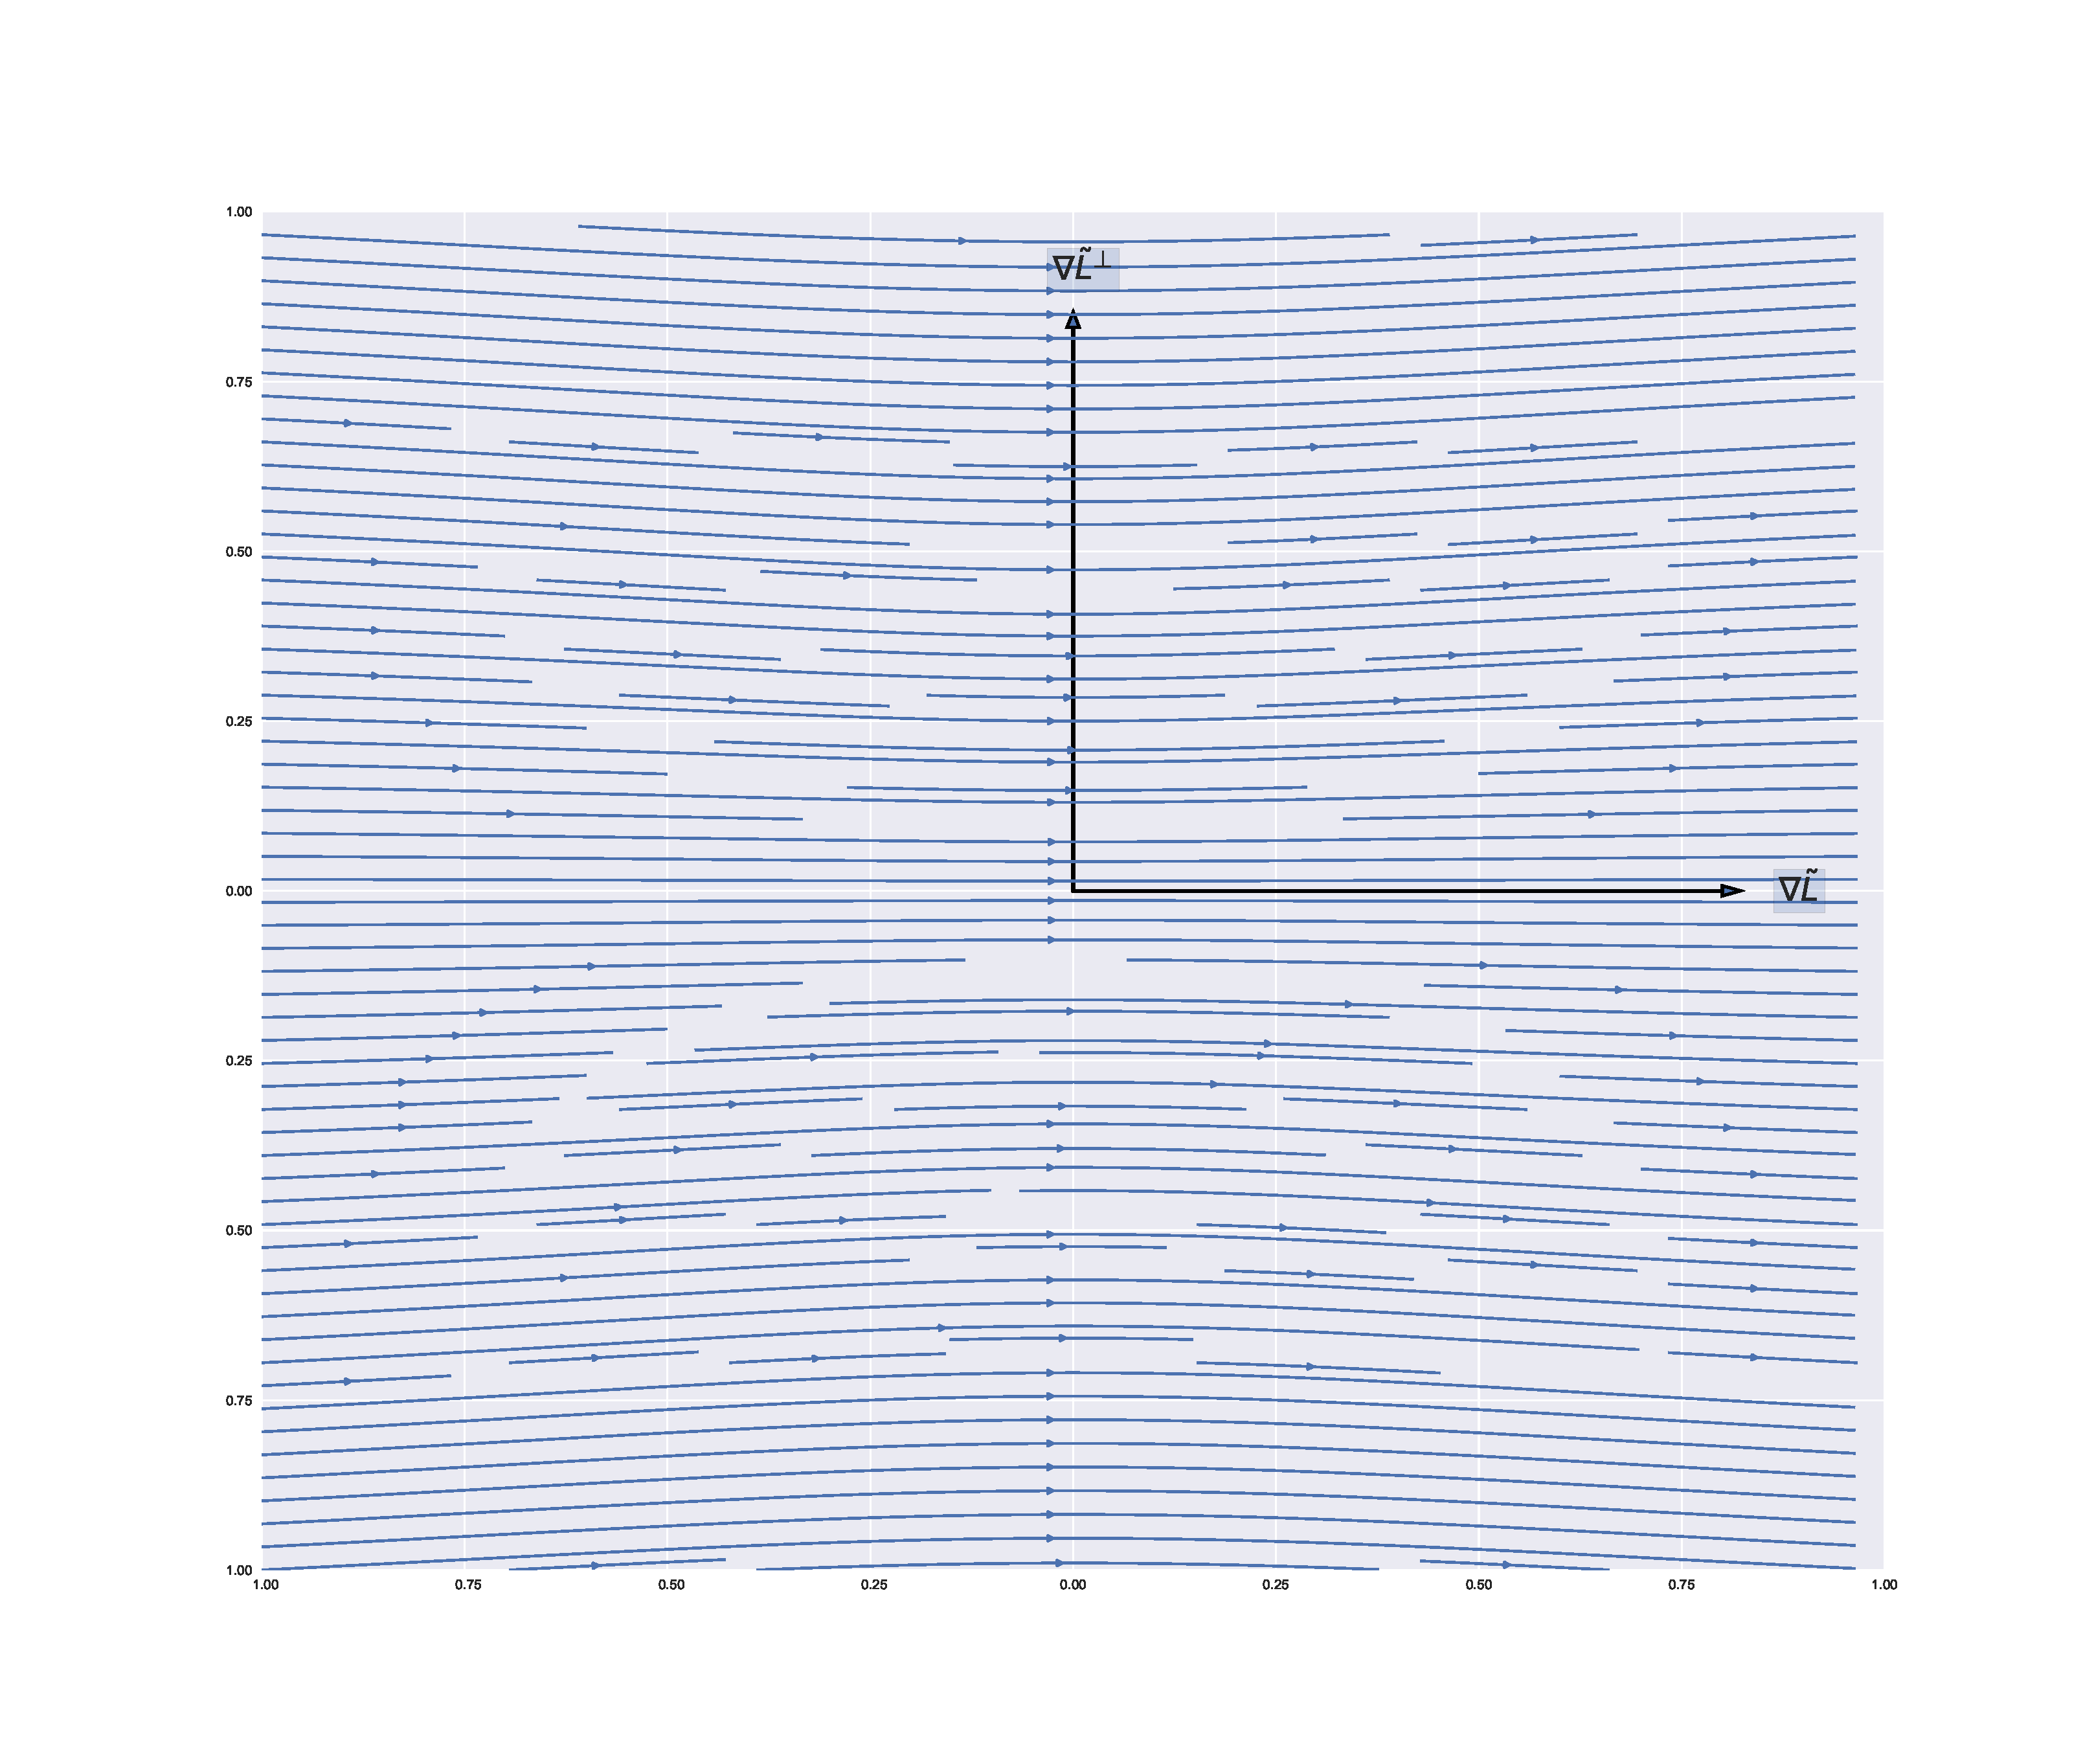
\includegraphics[width=\linewidth]{figures/dynamics_delta_1.pdf}
    % \endminipage\hfill
    \minipage{0.33\textwidth}
    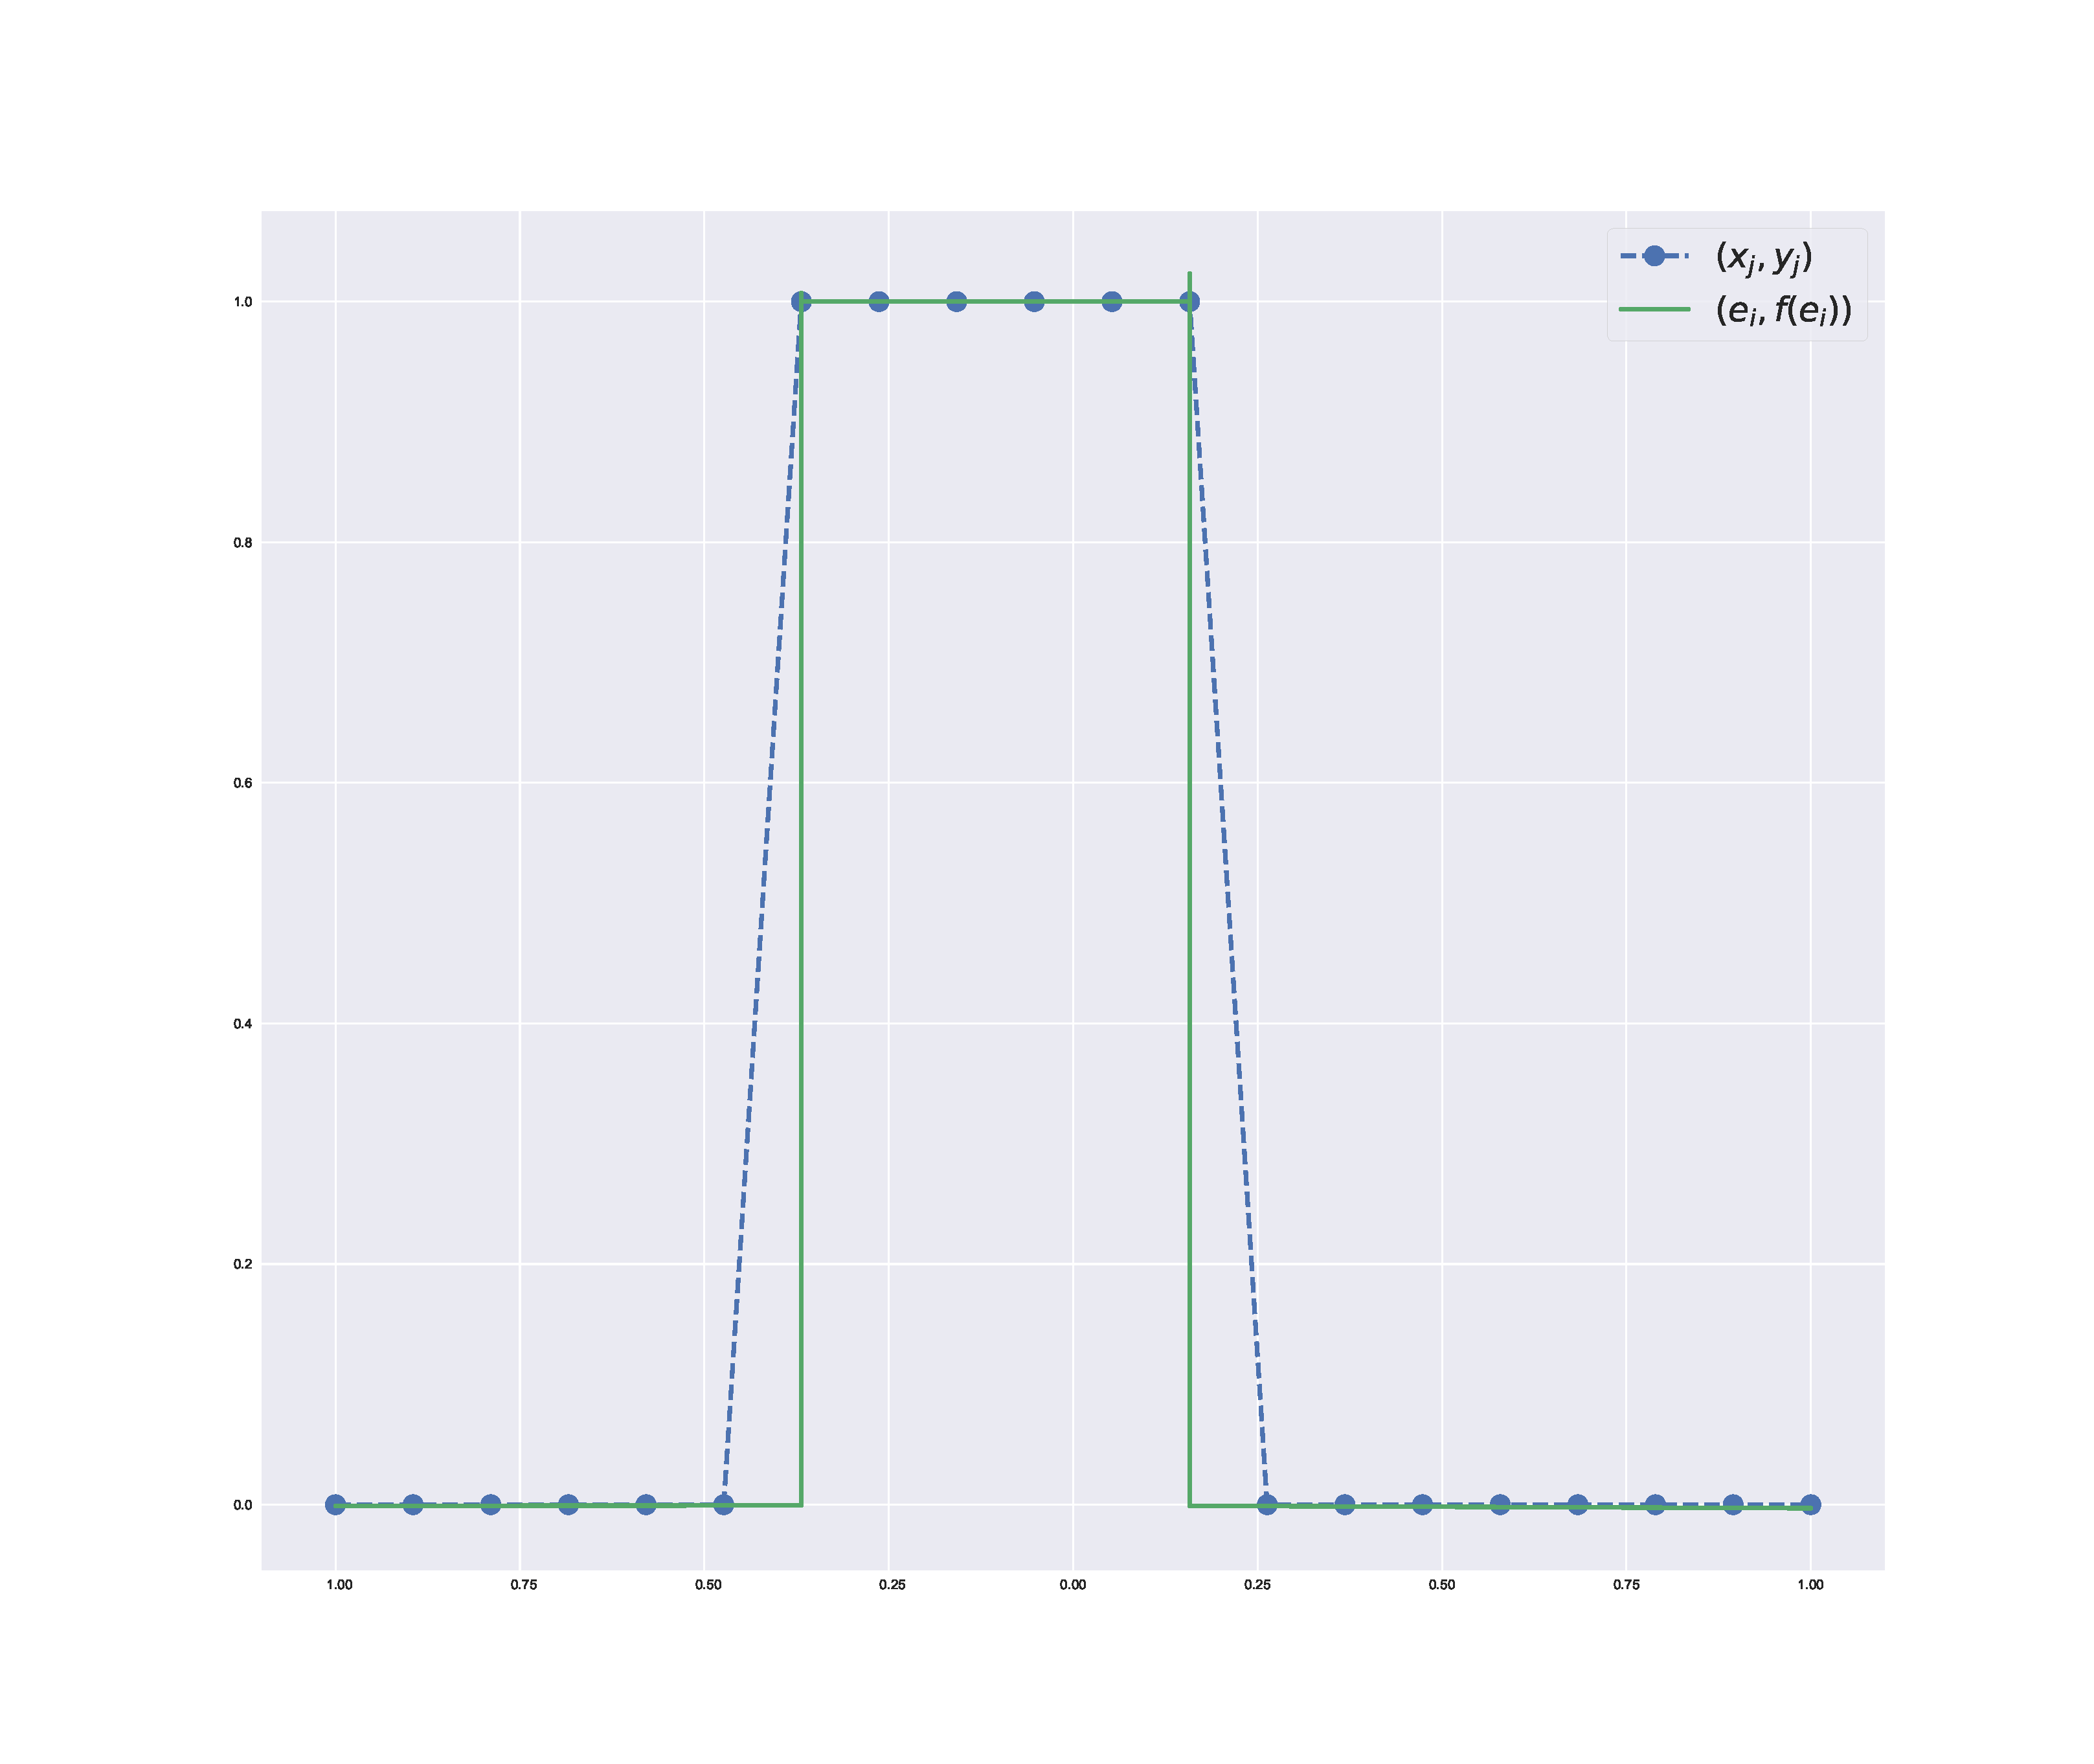
\includegraphics[width=\linewidth]{figures/same_init_different_func_square_1000.pdf}
    \endminipage
    
    \caption{The same initial function can yield very different results: the left image is the initial function for the two right ones. The initial parameters ($\bm a, \bm b, \bm c$) were the same as those in the middle image but scaled by a factor of 1000, 1000 and 0.001 respectively}
\end{figure}

% \begin{itemize}
%     \item If $c_i^2 \ll (a_i^2 + b_i^2)$, which means that $\delta <
%     0$, then $\xi_i'(t) \propto (u(t),v(t))$, and the reduced neuron
%     moves~\emph{radially} (\todo{Figure \ref{fig:todo}}).
%     \item If $c_i^2 \gg (a_i^2 + b_i^2)$, which means that $\delta > 0$, then
%     $\xi_i'(t) \propto \nabla \tilde L(\xi)_i$, so the reduced neuron follows the gradient field $\nabla \tilde{L}$ (\todo{Figure \ref{fig:todo}}).
% \end{itemize}


% The shapes of a neuron's trajectory is thus controlled by the invariant $\delta_i$ which can be altered by re-scaling the gradient flow (changing $\alpha$ or $\beta$), or changing the initial distribution from which the parameters $\theta = (a, b, c)$ are sampled. 




\begin{remark}
\note{Discuss relationship with asymptotics of other works.}
\end{remark}

If $\rho_i \ll |\delta_i|$ holds for all neurons, then we say that we are in the regime of \emph{kernel learning}; similarly if $\rho_i \gg |\delta_i|$ holds for all neurons we are in the regime of \emph{purely adaptive learning}. In the next section, we study the dynamics in these two extreme regimes.
In particular, we study how the two extrema above bias the network to very different kinds of solutions: kernel learning motion biases towards smooth solutions, while purely adaptive learning biases towards piecewise linear solutions. 

\begin{remark}
The kernel and purely adaptive regimes are related to the kernel dynamics \eqref{eq:tangent_kernel}. Kernel Learning corresponds to the function only evolving along $\bm K^c$ and Adaptive Learning corresponds to evolution along $\bm K^{ab}$.  
\end{remark}










\subsection{Kernel Learning}
We first consider the regime of kernel learning, where $\delta_i \ll -\|\xi_i\|$. In this regime, reduced neurons move radially away from the origin (see Figure \ref{fig:trajectories}). These trajectories are equivalent to training only the outer-layer parameters ($\bm c$) while keeping the inner-layer parameters ($\bm a, \bm b$) fixed. In the overparameterized case, this corresponds to the least squares problem
\begin{equation}\label{eq:least_squares_op}
    \text{minimize } \|\bm c\|^2 \text{ s.t. } f_{\bm \theta}(x) = \bm M_{ab} \bm c = \bm y
\end{equation}

Solutions $f(x)$ can be written in terms of the kernel (\todo{see supplemental sections ...})
\begin{equation}
\begin{gathered}
    f(x) = \sum_{j=1}^s \alpha_j K(x_j, x) \text{ where } \\
    K(x, x') = \sum_{i=1}^m [a_i x + b_i]_+ [a_i x' + b_i]_+ \text{ and } \alpha_j = (\bm K_c^{-1} \bm y)_j  
\end{gathered}
\end{equation}

Note that $K(x_i, x_j) = \bm K_{c, ij}$. Also note that gradient flow will converge to this solution only if $\bm c(0)$ is initialized sufficiently close to the origin. To understand solutions to \eqref{eq:least_squares_op}, we consider the $K$ as an approximation of the the network in the limit as the number of neurons goes to infinity ($m \rightarrow \infty$). In this case, the parameters $\bm \theta_i$ become functions $\bm \theta(s)$. Assuming the domain of $f$ is $[k_1, k_2]$, as $m \rightarrow \infty$ we have that

\begin{equation}
    K(x, x') = \int_{k_1}^{k_2} [a(s)x + b(s)]_+ [a(s)x' + b(s)]_+ ds
\end{equation}

\begin{lemma}\label{le:curvature_minimizer}
In this infinite width limit ($m = \infty$), $c(s) = \partial_x^2 f(x)$
\end{lemma}

Thus solutions to the least squares problem \eqref{eq:least_squares_op} minimize \emph{curvature} subject to equality constraints. 
\begin{lemma}\label{le:cubic_poly}
When $m = \infty$ and $\bm \theta(s) ~ \lambda U(-1, 1)$ are initialized from a uniform distribution, then the function $K(x, x')$ is a cubic polynomial in $x$ and $x'$.
\end{lemma}

We remark that machine learning packages such as PyTorch use a uniform distribution for linear layer parameter initialization by default.

\begin{corollary}
A corollary of Lemmas~\ref{le:curvature_minimizer}~and~\ref{le:cubic_poly} are that solutions to the gradient flow with $\|c(0)\| = 0$ are cubic splines. 
\end{corollary}

We verify that indeed, solutions to \eqref{eq:leastsquares} converge to cubic splines as $m$ grows in Figure~\ref{fig:cubic_splines}. We also point out that in Kernel Learning, early termination of gradient flow acts as a regularizer favoring smooth, non-interpolatory solutions (see \cite{NTKJacot} and \todo{Section~\ref{sec:todo}} of the supplementary).



\subsection{Purely Adaptive Learning}
We now consider the Purely Adaptive regime where $\delta_i \ll \| \xi_i \|$. In this regime, neurons move parallel to the reduced gradient field $\nabla \tilde{L}(\bm \xi)$ (see Figure \ref{fig:trajectories}). These trajectories are equivalent to those when training only the bottom layer parameters $(\bm a, \bm b)$ while keeping the top layer ($\bm c$) fixed. To understand the dynamics in this regime, we write the function $f$ in terms of the reduced parameters

\begin{equation}
    f_{\bm \xi}(x) = \sum_{i=1}^m \langle (x, 1), (u_i, v_i) \rangle_+ 
\end{equation}

The gradient of the loss with respect to the reduced parameters is 
\begin{equation}\label{eq:grad_reduced}
    \nabla \tilde{L}(\bm \xi)_i = \sum_{i=1}^s (f_{\bm \xi}(x_j) - y_j) \epsilon_i \tau_{ij} \begin{bmatrix}x_j \\ 1\end{bmatrix} 
\end{equation}

\begin{figure}
    \centering
    \minipage{0.33\textwidth}
        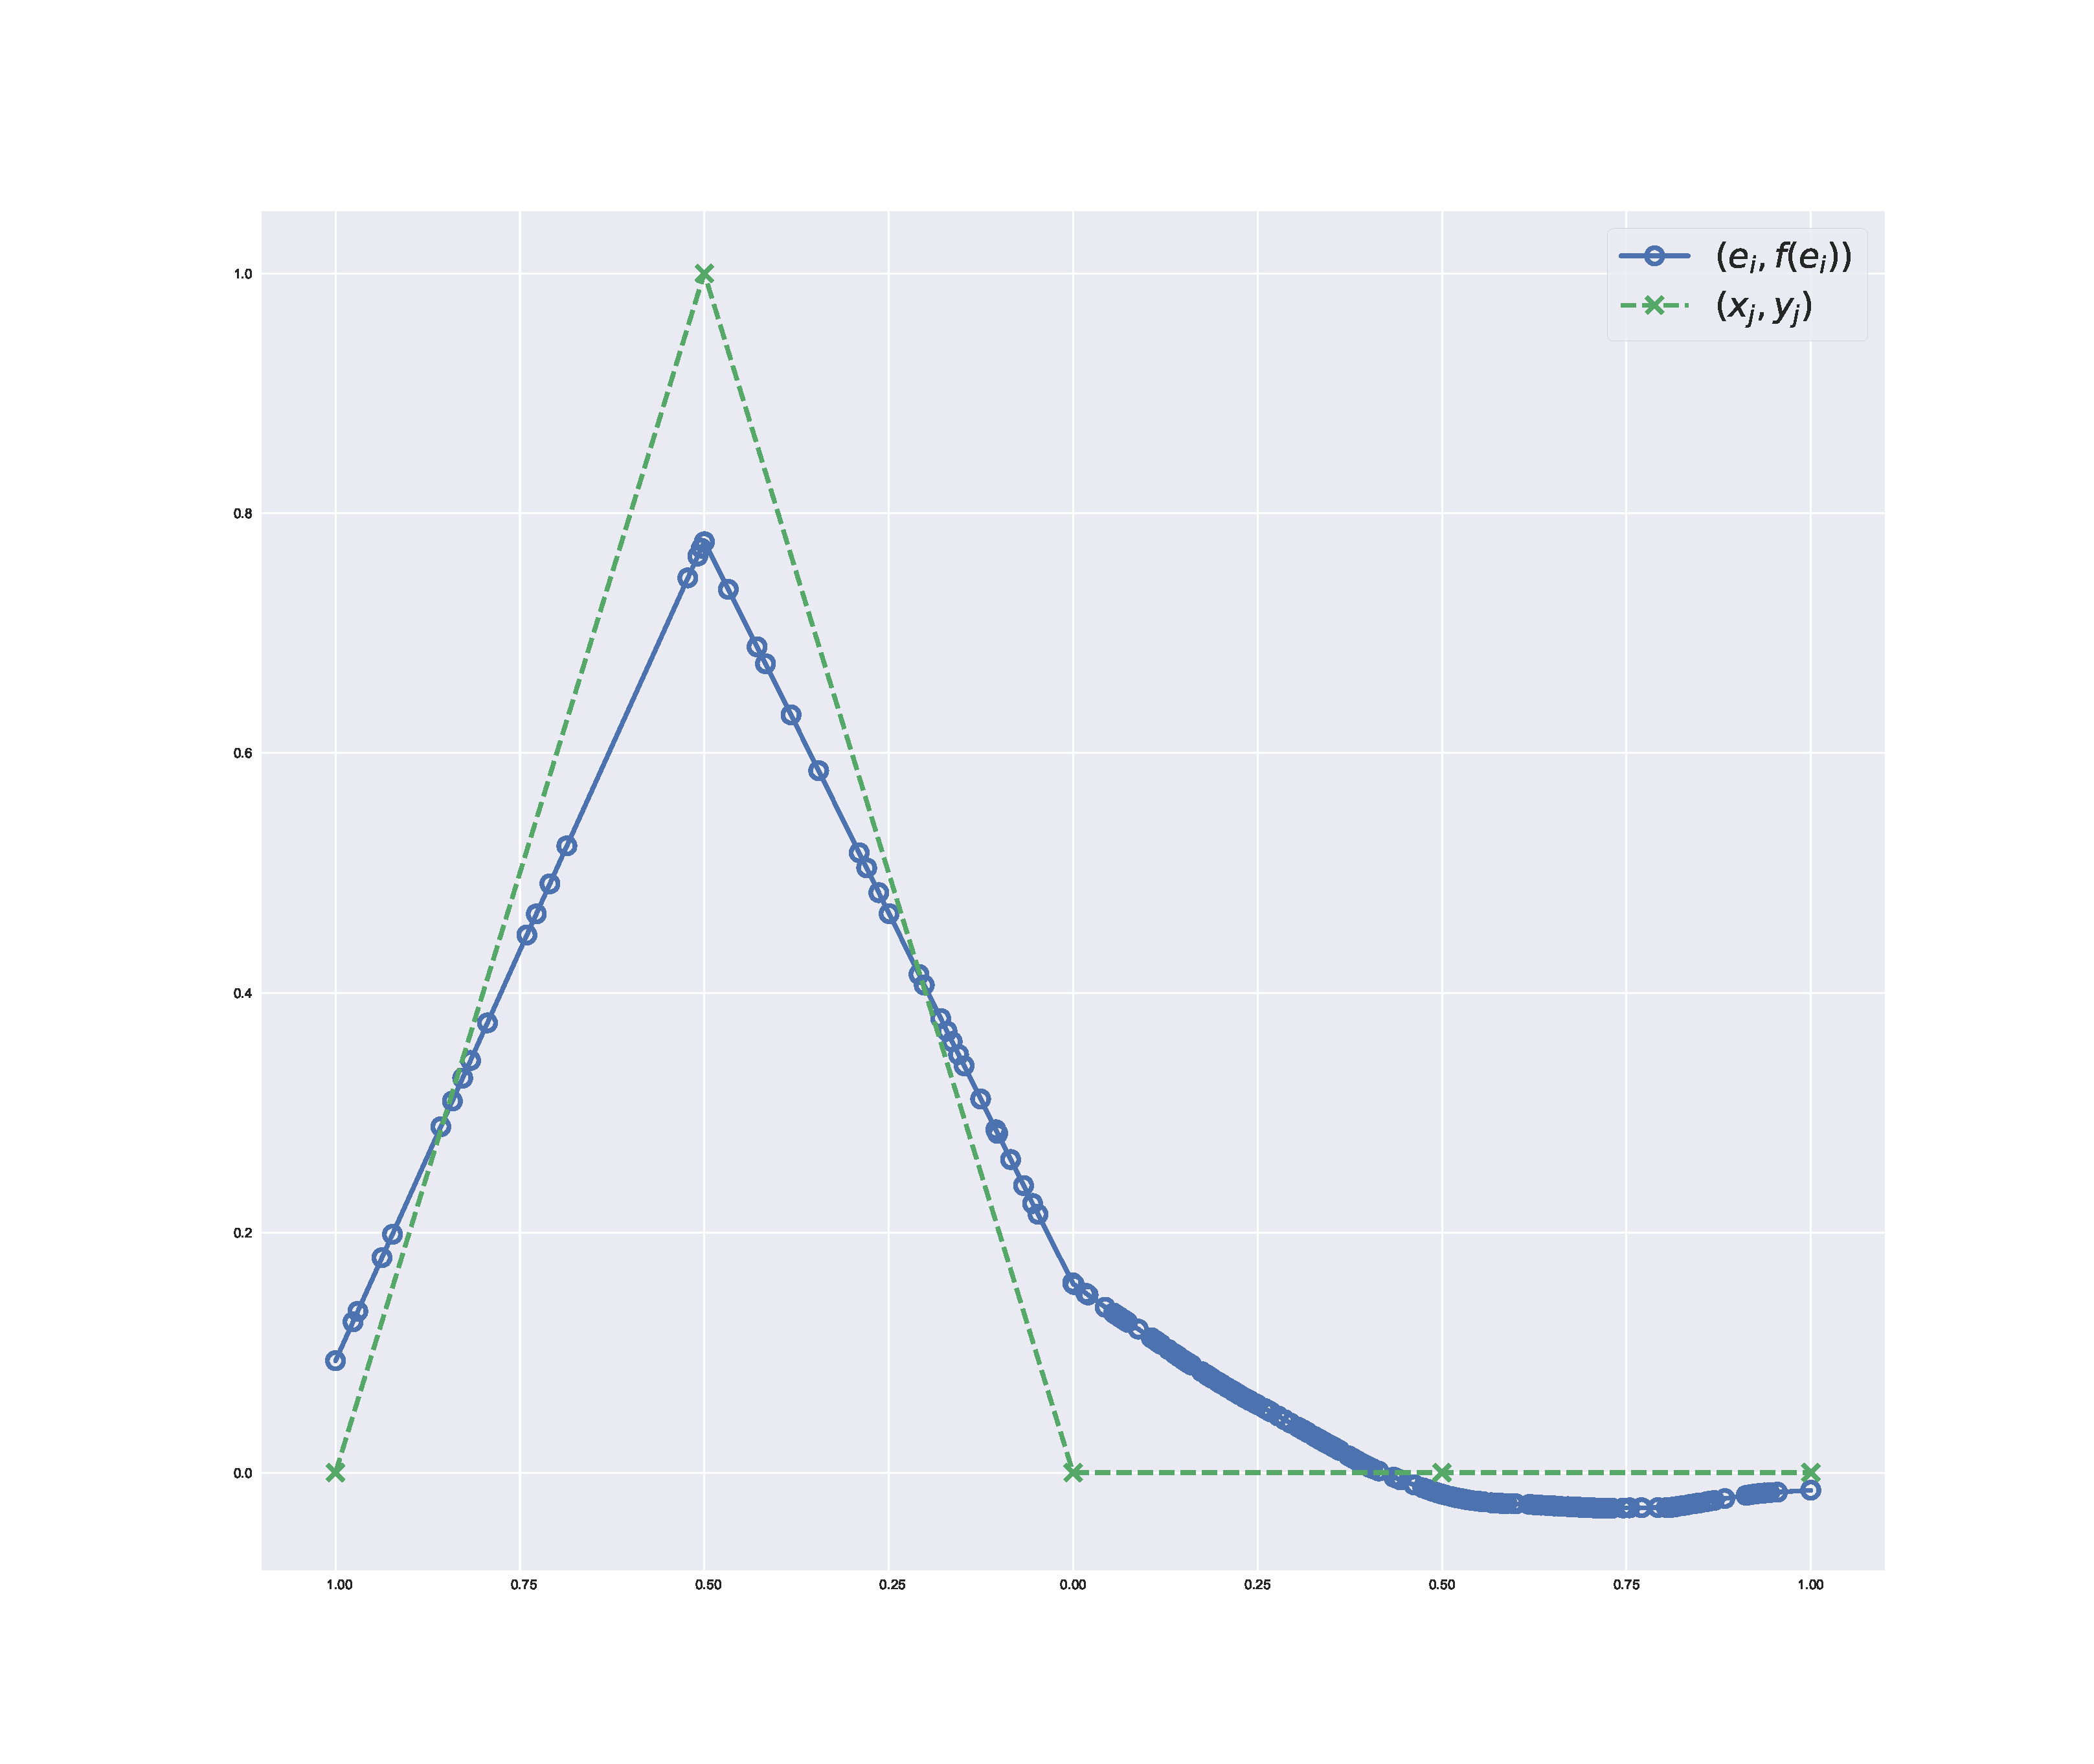
\includegraphics[width=\linewidth]{figures/reduced_gradient_recon.pdf}
    \endminipage
    \minipage{0.33\textwidth}
        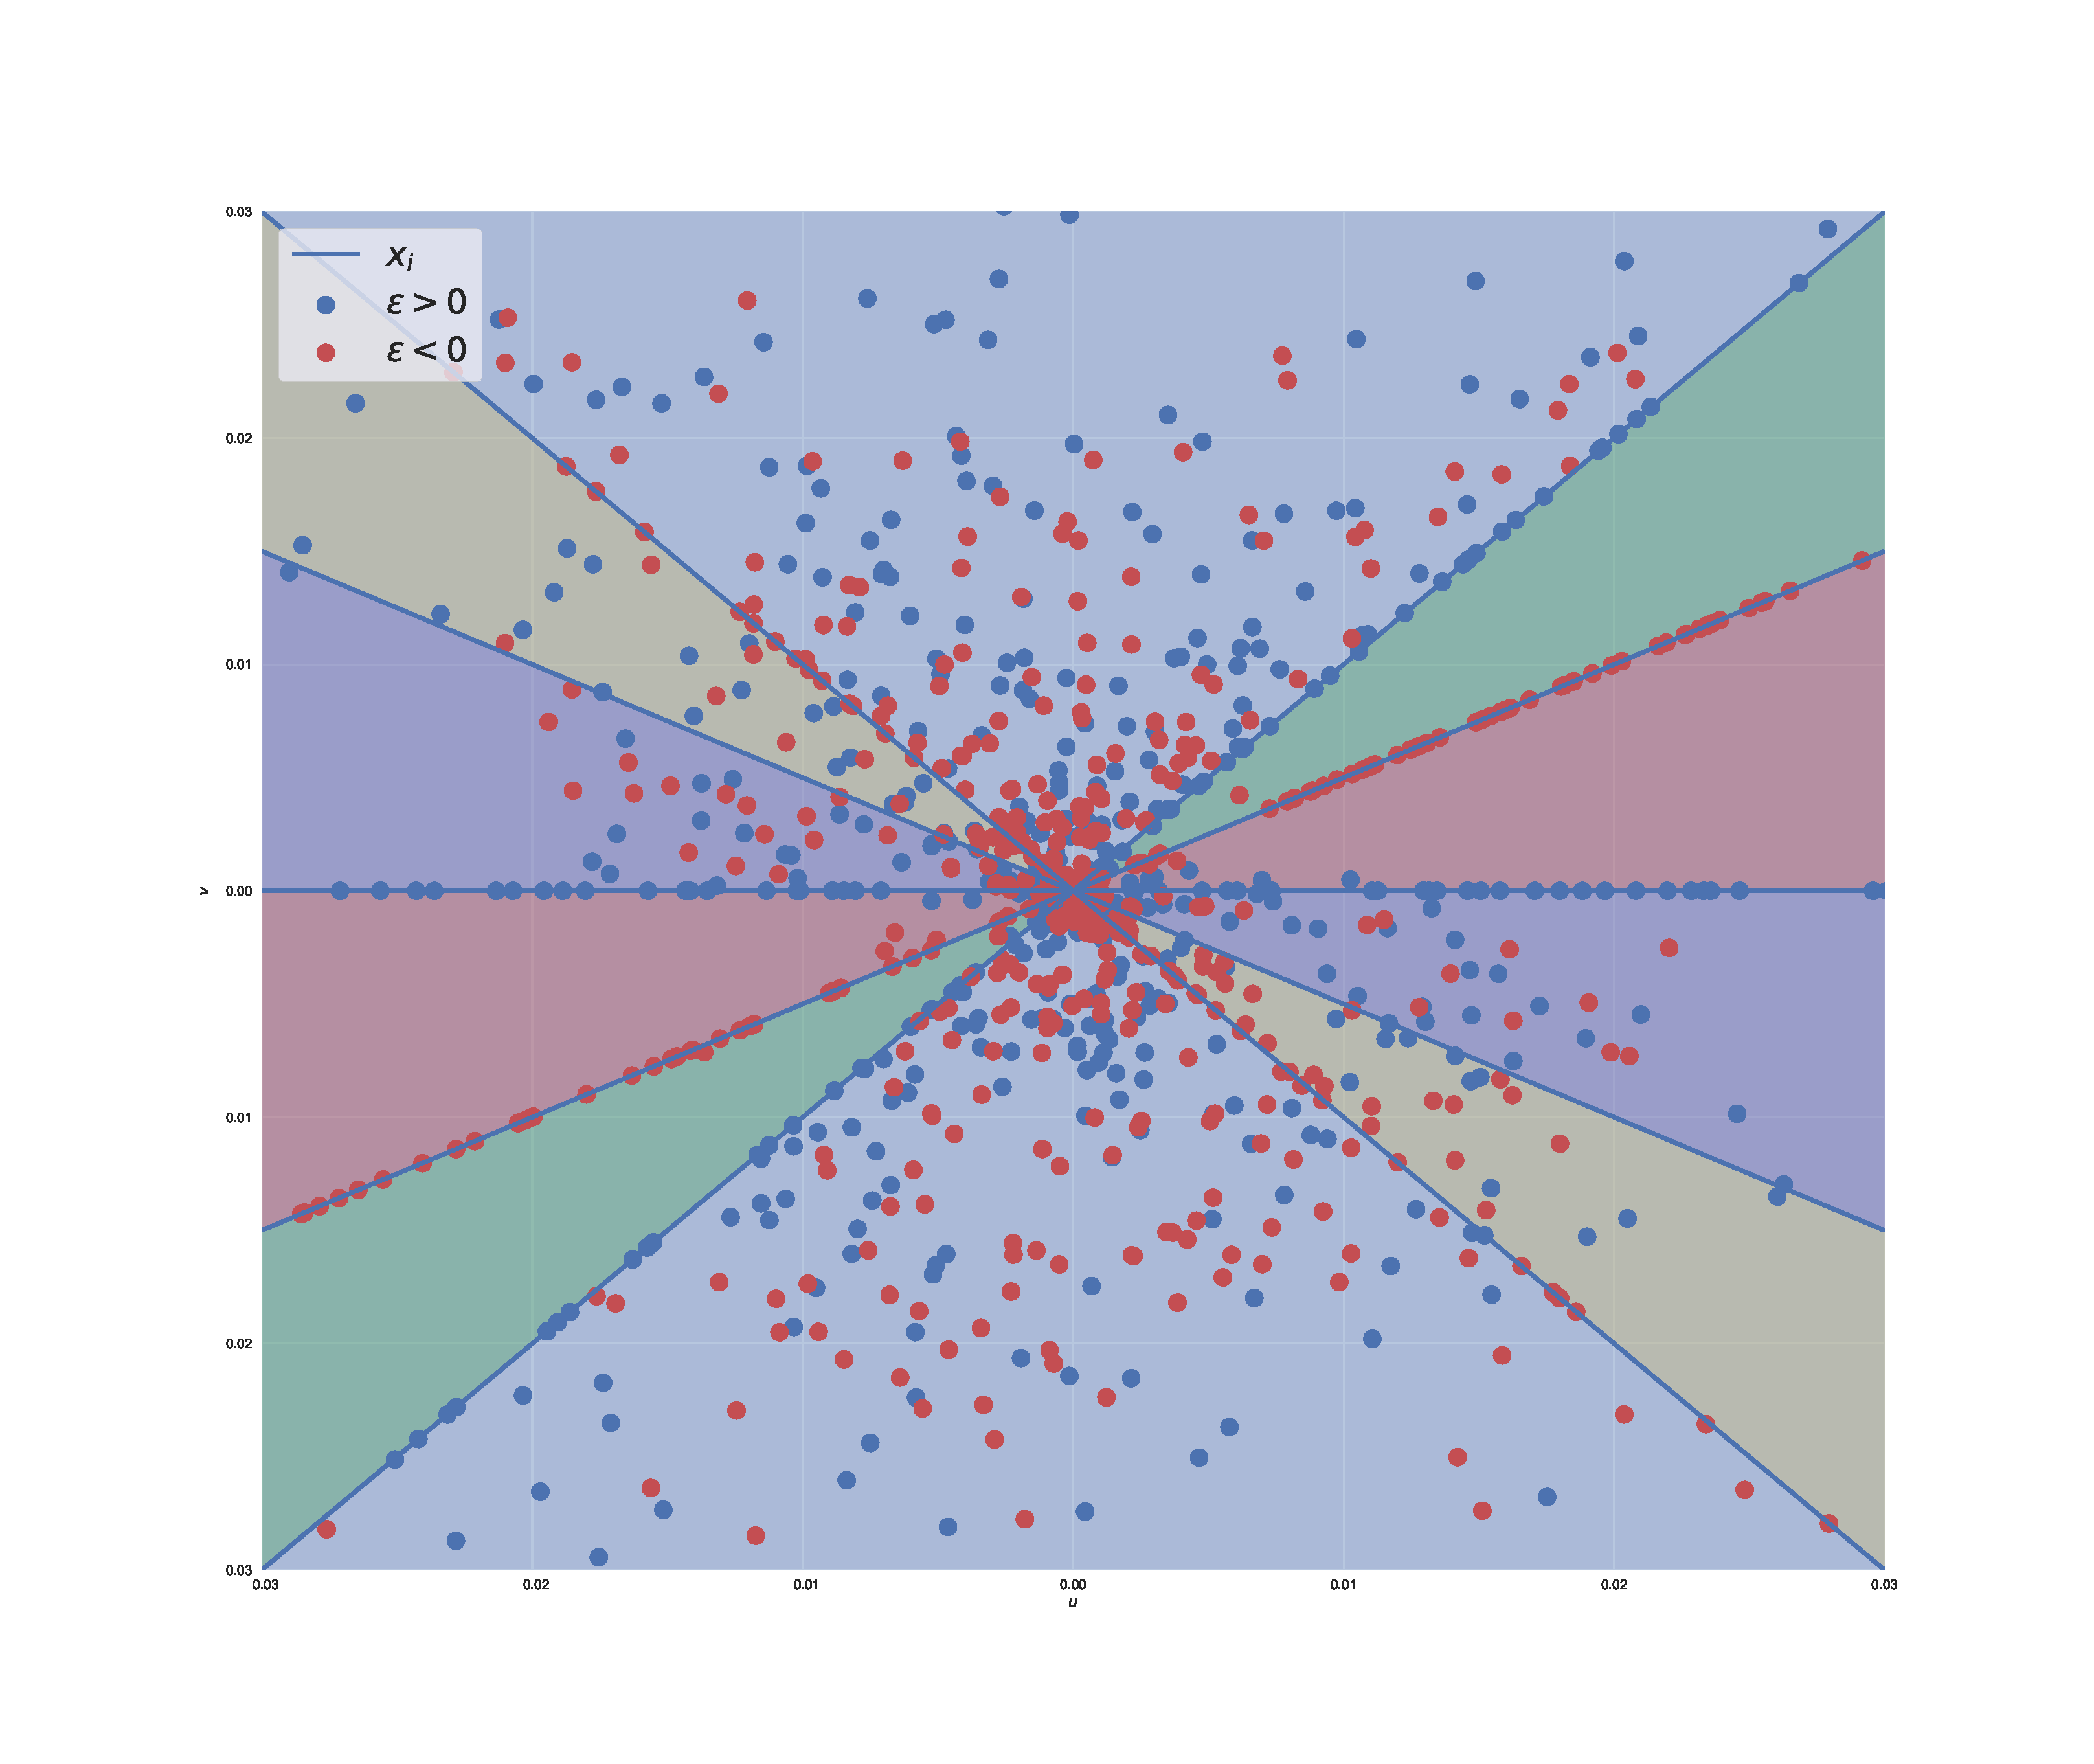
\includegraphics[width=\linewidth]{figures/reduced_gradient_phase.pdf}
    \endminipage
    \minipage{0.33\textwidth}
        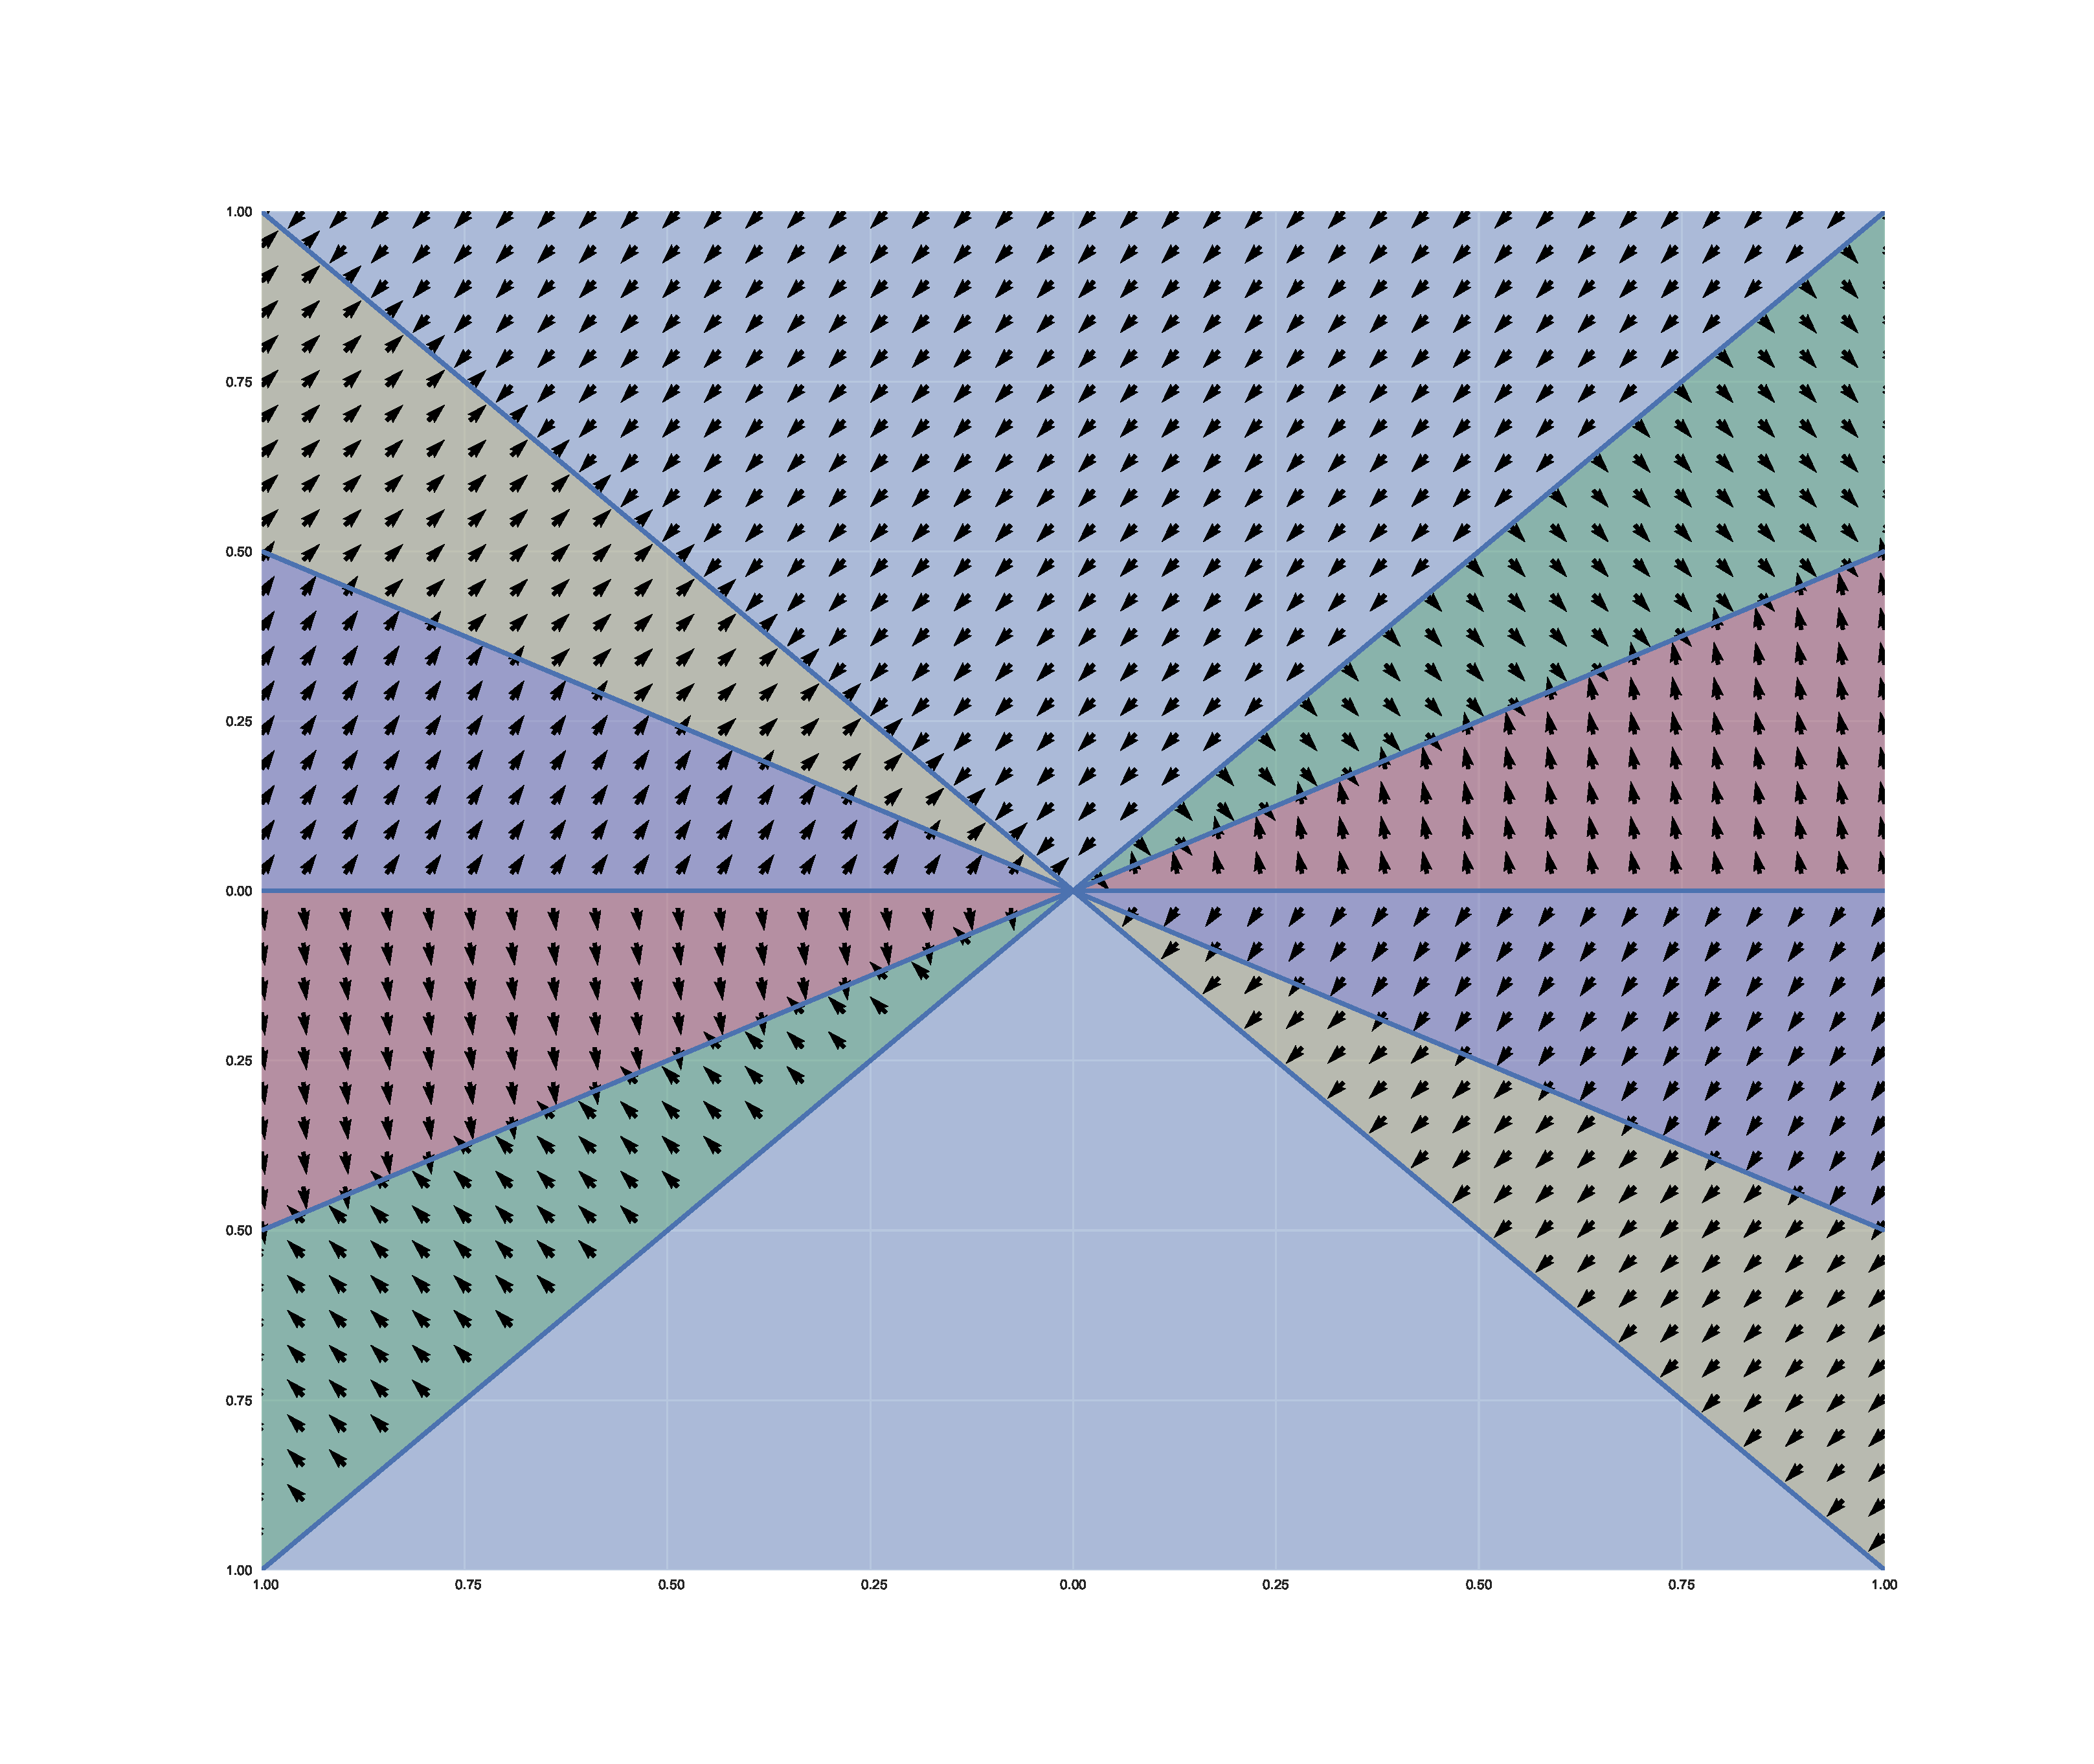
\includegraphics[width=\linewidth]{figures/reduced_gradient_vector_field.pdf}
    \endminipage\hfill
    \caption{The vector field of the gradient of the loss in reduced parameter space $\nabla \tilde{L}(\bm \xi)$. Note that the orientation of the arrow depends on the sign $\epsilon_i$ of a neuron. Thus, the gradient of the blue neurons are the arrows in the picture while the gradient of the red neurons point point in the opposite direction. We see in the middle image, that the neurons cluster on different samples depending on their sign.}
    \label{fig:reduced_grad}
\end{figure}

which is a piecewise constant function with the boundary between pieces occuring along the sample lines $u x_j + v = 0, j = 1 \ldots s$ (see Figure~\ref{fig:reduced_grad}). While the gradient field is in general discontinuous on the boundary of a sample, the component along a sample line is continuous

\begin{lemma}
The component of the gradient field $\nabla \tilde{L}(\xi)$ along a line $l : u x_j + v = 0$ is continuous in any open neighborhood centered on $l$.
\end{lemma}

We see from \eqref{eq:grad_reduced} that $\nabla \tilde{L}$ at a point $(u_i, v_i, \epsilon_i)$ is a linear combination of the sample vectors $(x_j, 1)^T$  weighted by the residual $f_{\bm \xi}(x_j) - y_j$ with a possible sign flip depending on $\epsilon_i$. Thus depending on $\epsilon_i$ and the signs of the residuals at the samples, $\nabla \tilde{L}$ for a specific neuron could point in opposing directions along a sample boundary. In the cases, where the vector field points towards the sample line on either side, neurons will ``stick'' to the sample boundary. In fact, we show that for every possible neuron, there is at least one ``sticky'' sample to which it is attracted. Note that these ''sticky`` samples may change over time as the residual evolves and as the signs of neurons change. Below we give a condition for a sample to be attract a neuron. 

\begin{lemma}
Given a set of samples $\bm x = (x_j)_{j=1}^s$ and labels $\bm y = (y_j)_{j=1}^s$, then for any given residual and sign $\epsilon$, there is a nonempty set $S$ of samples $x_j$ which are sticky. \note{(this is super informal but I want to get a quick draft of the section, we should write out explicitly that the gradient field along the sample boundary is pointing in opposite directions )}
\end{lemma}

\todo{The attractiveness of samples only depends on the number of samples, neurons concentrate along sample lines , condition for attractiveness, clustering acts as a regularizer favoring piecewise linear functions.}
\begin{figure}
    \centering
    \minipage{0.33\textwidth}
    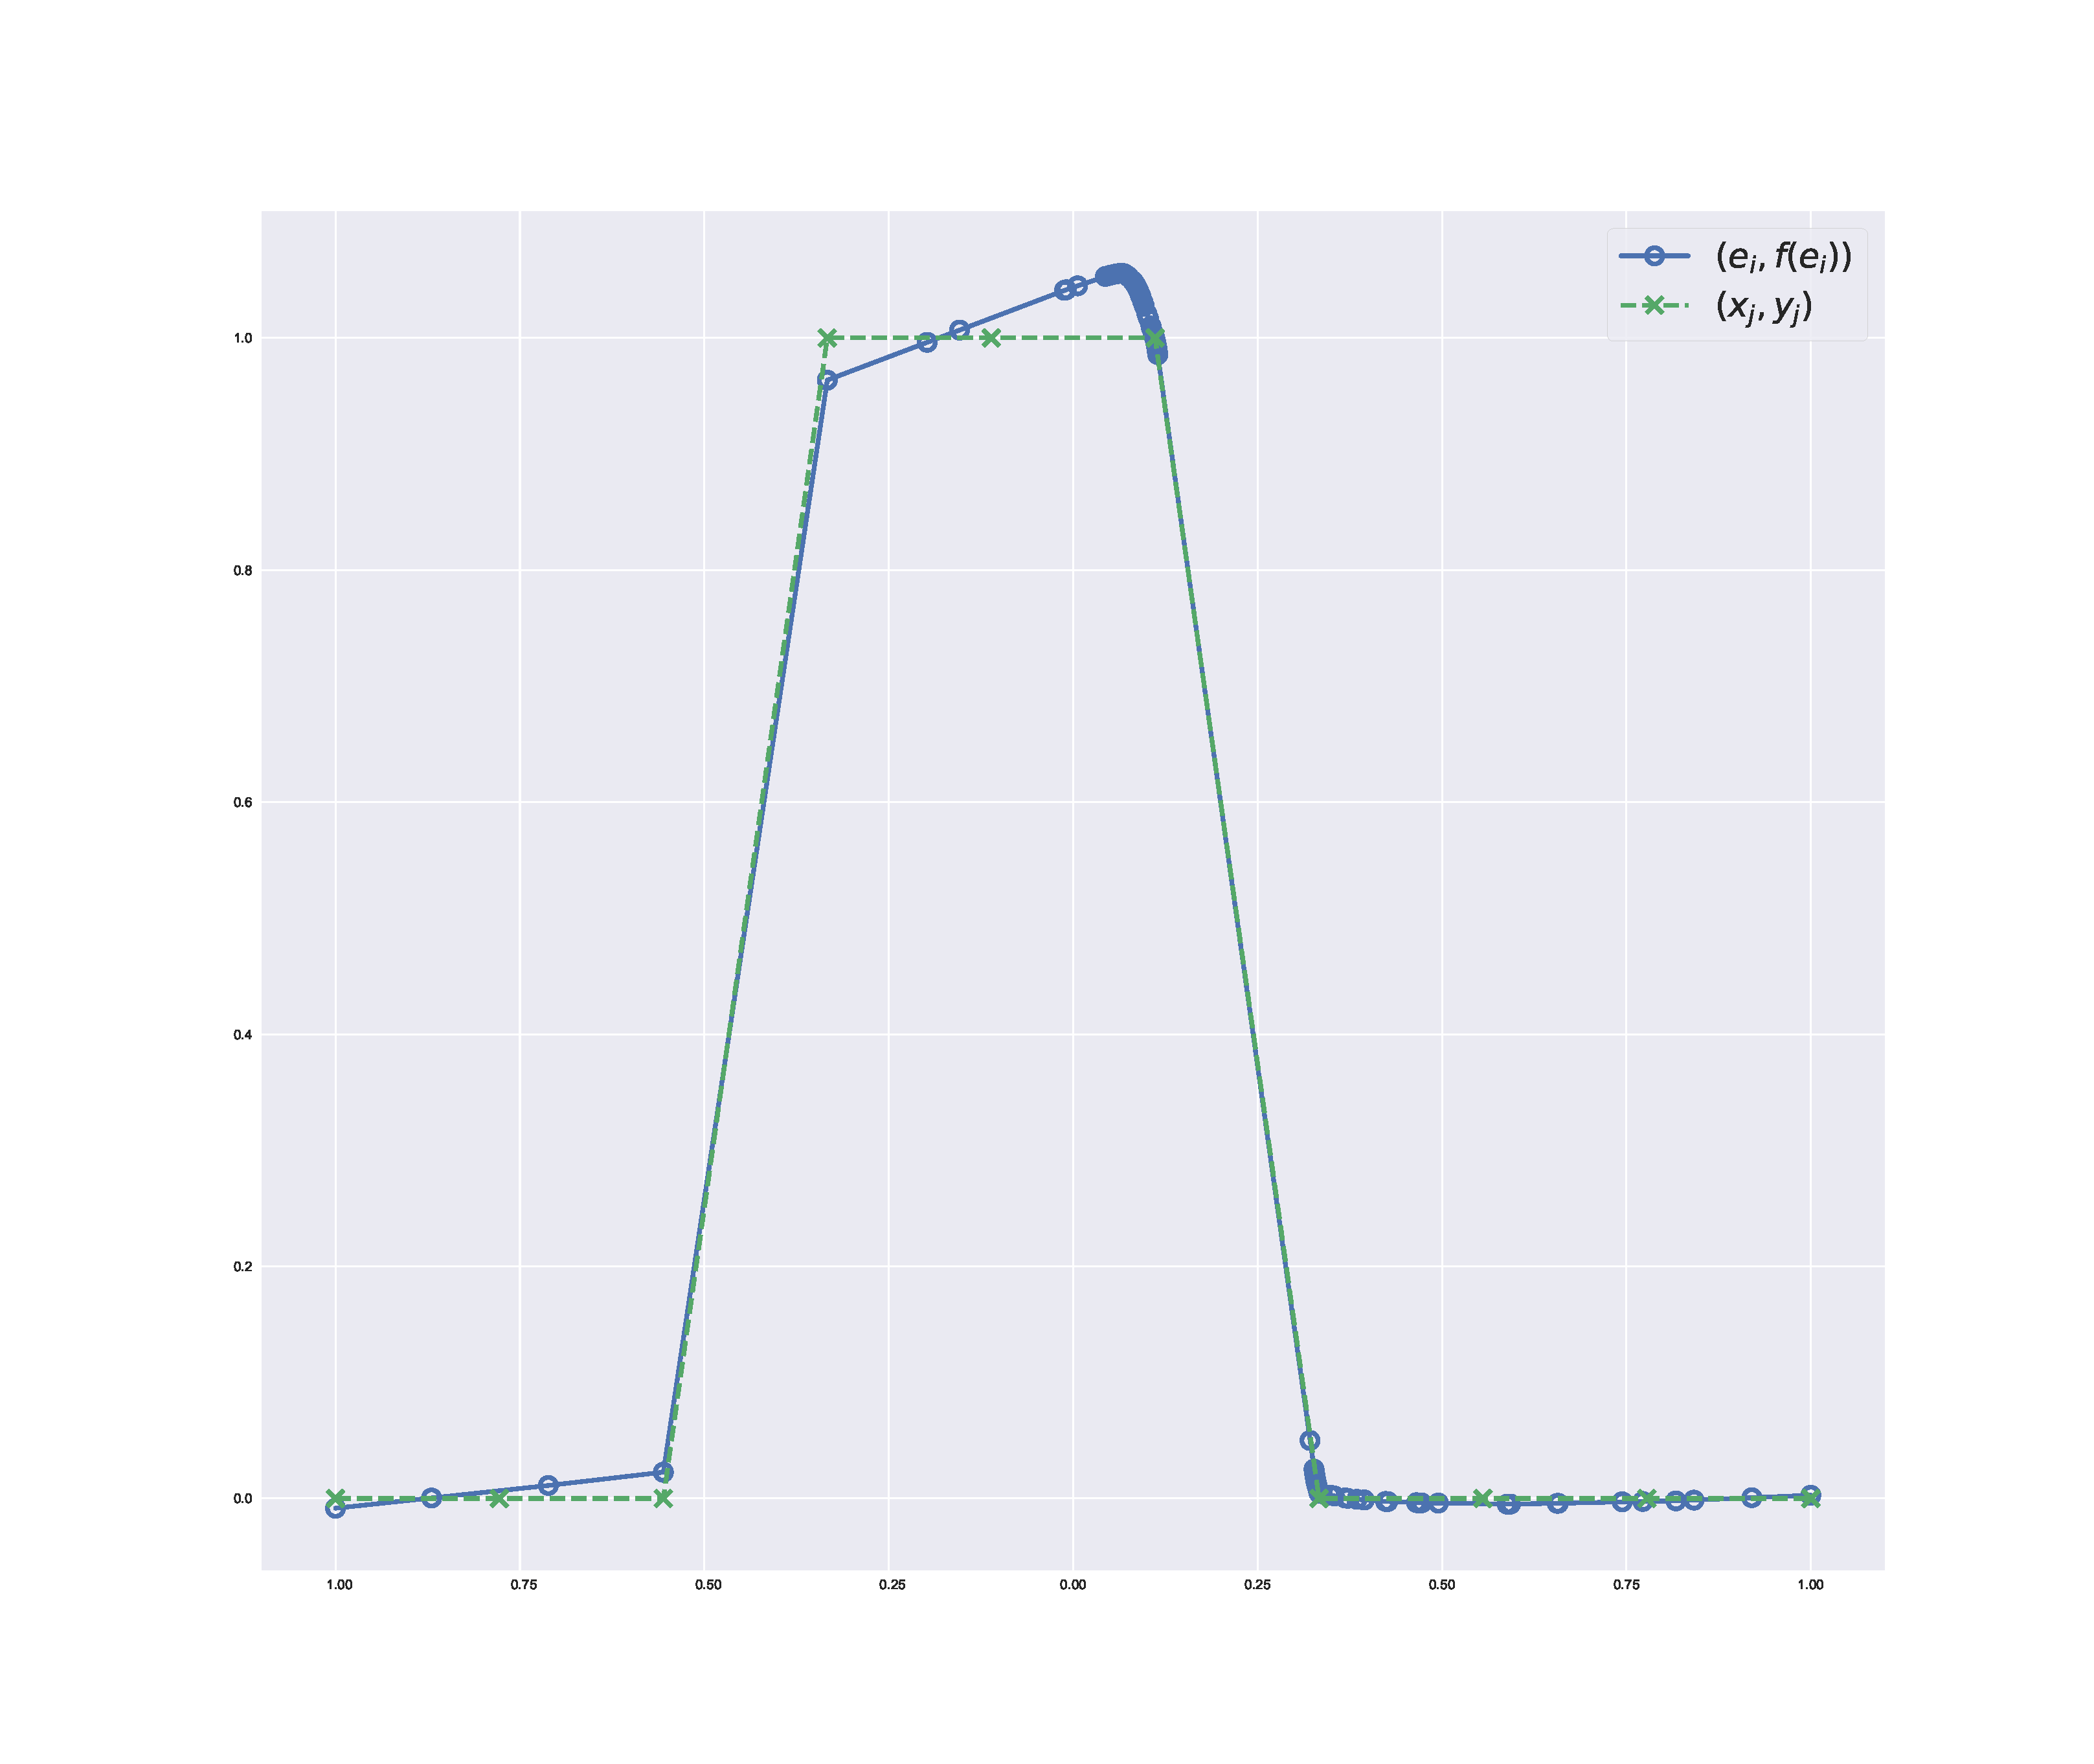
\includegraphics[width=\linewidth]{figures/neuron_trajectories_recon.pdf}
    \endminipage\hfill
    \minipage{0.33\textwidth}
    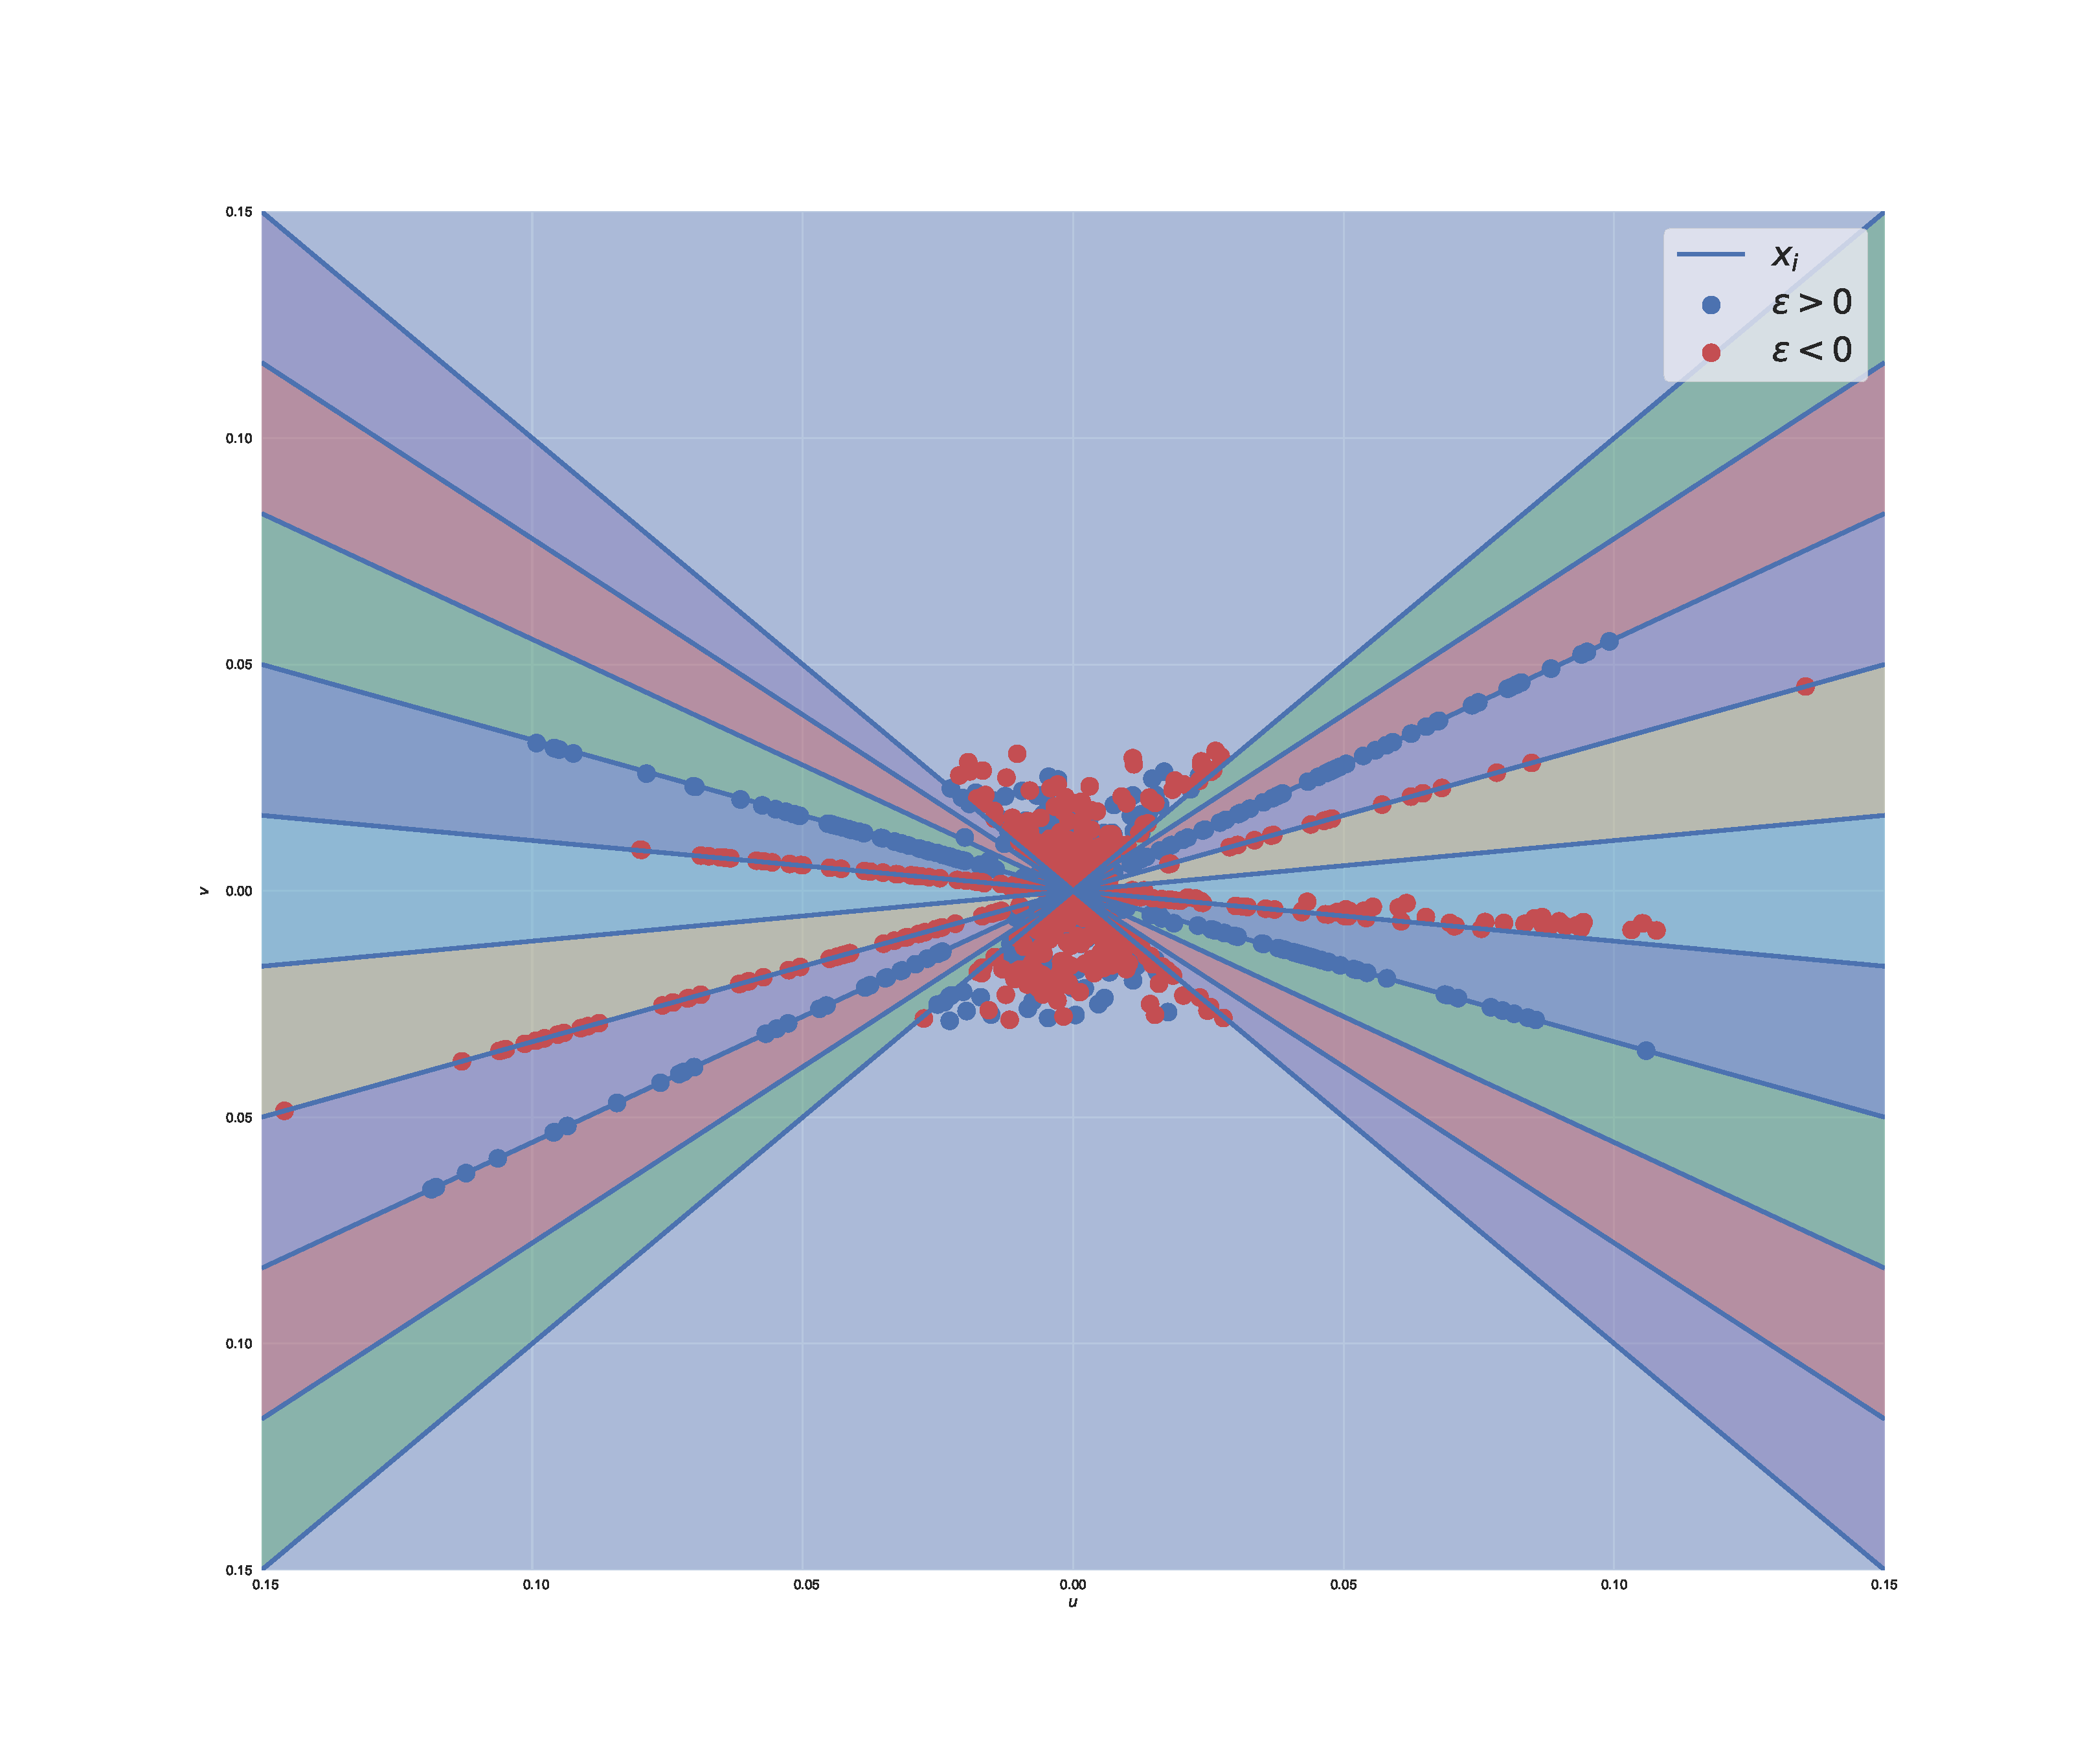
\includegraphics[width=\linewidth]{figures/neuron_trajectories_phase.pdf}
    \endminipage\hfill
    \minipage{0.33\textwidth}
    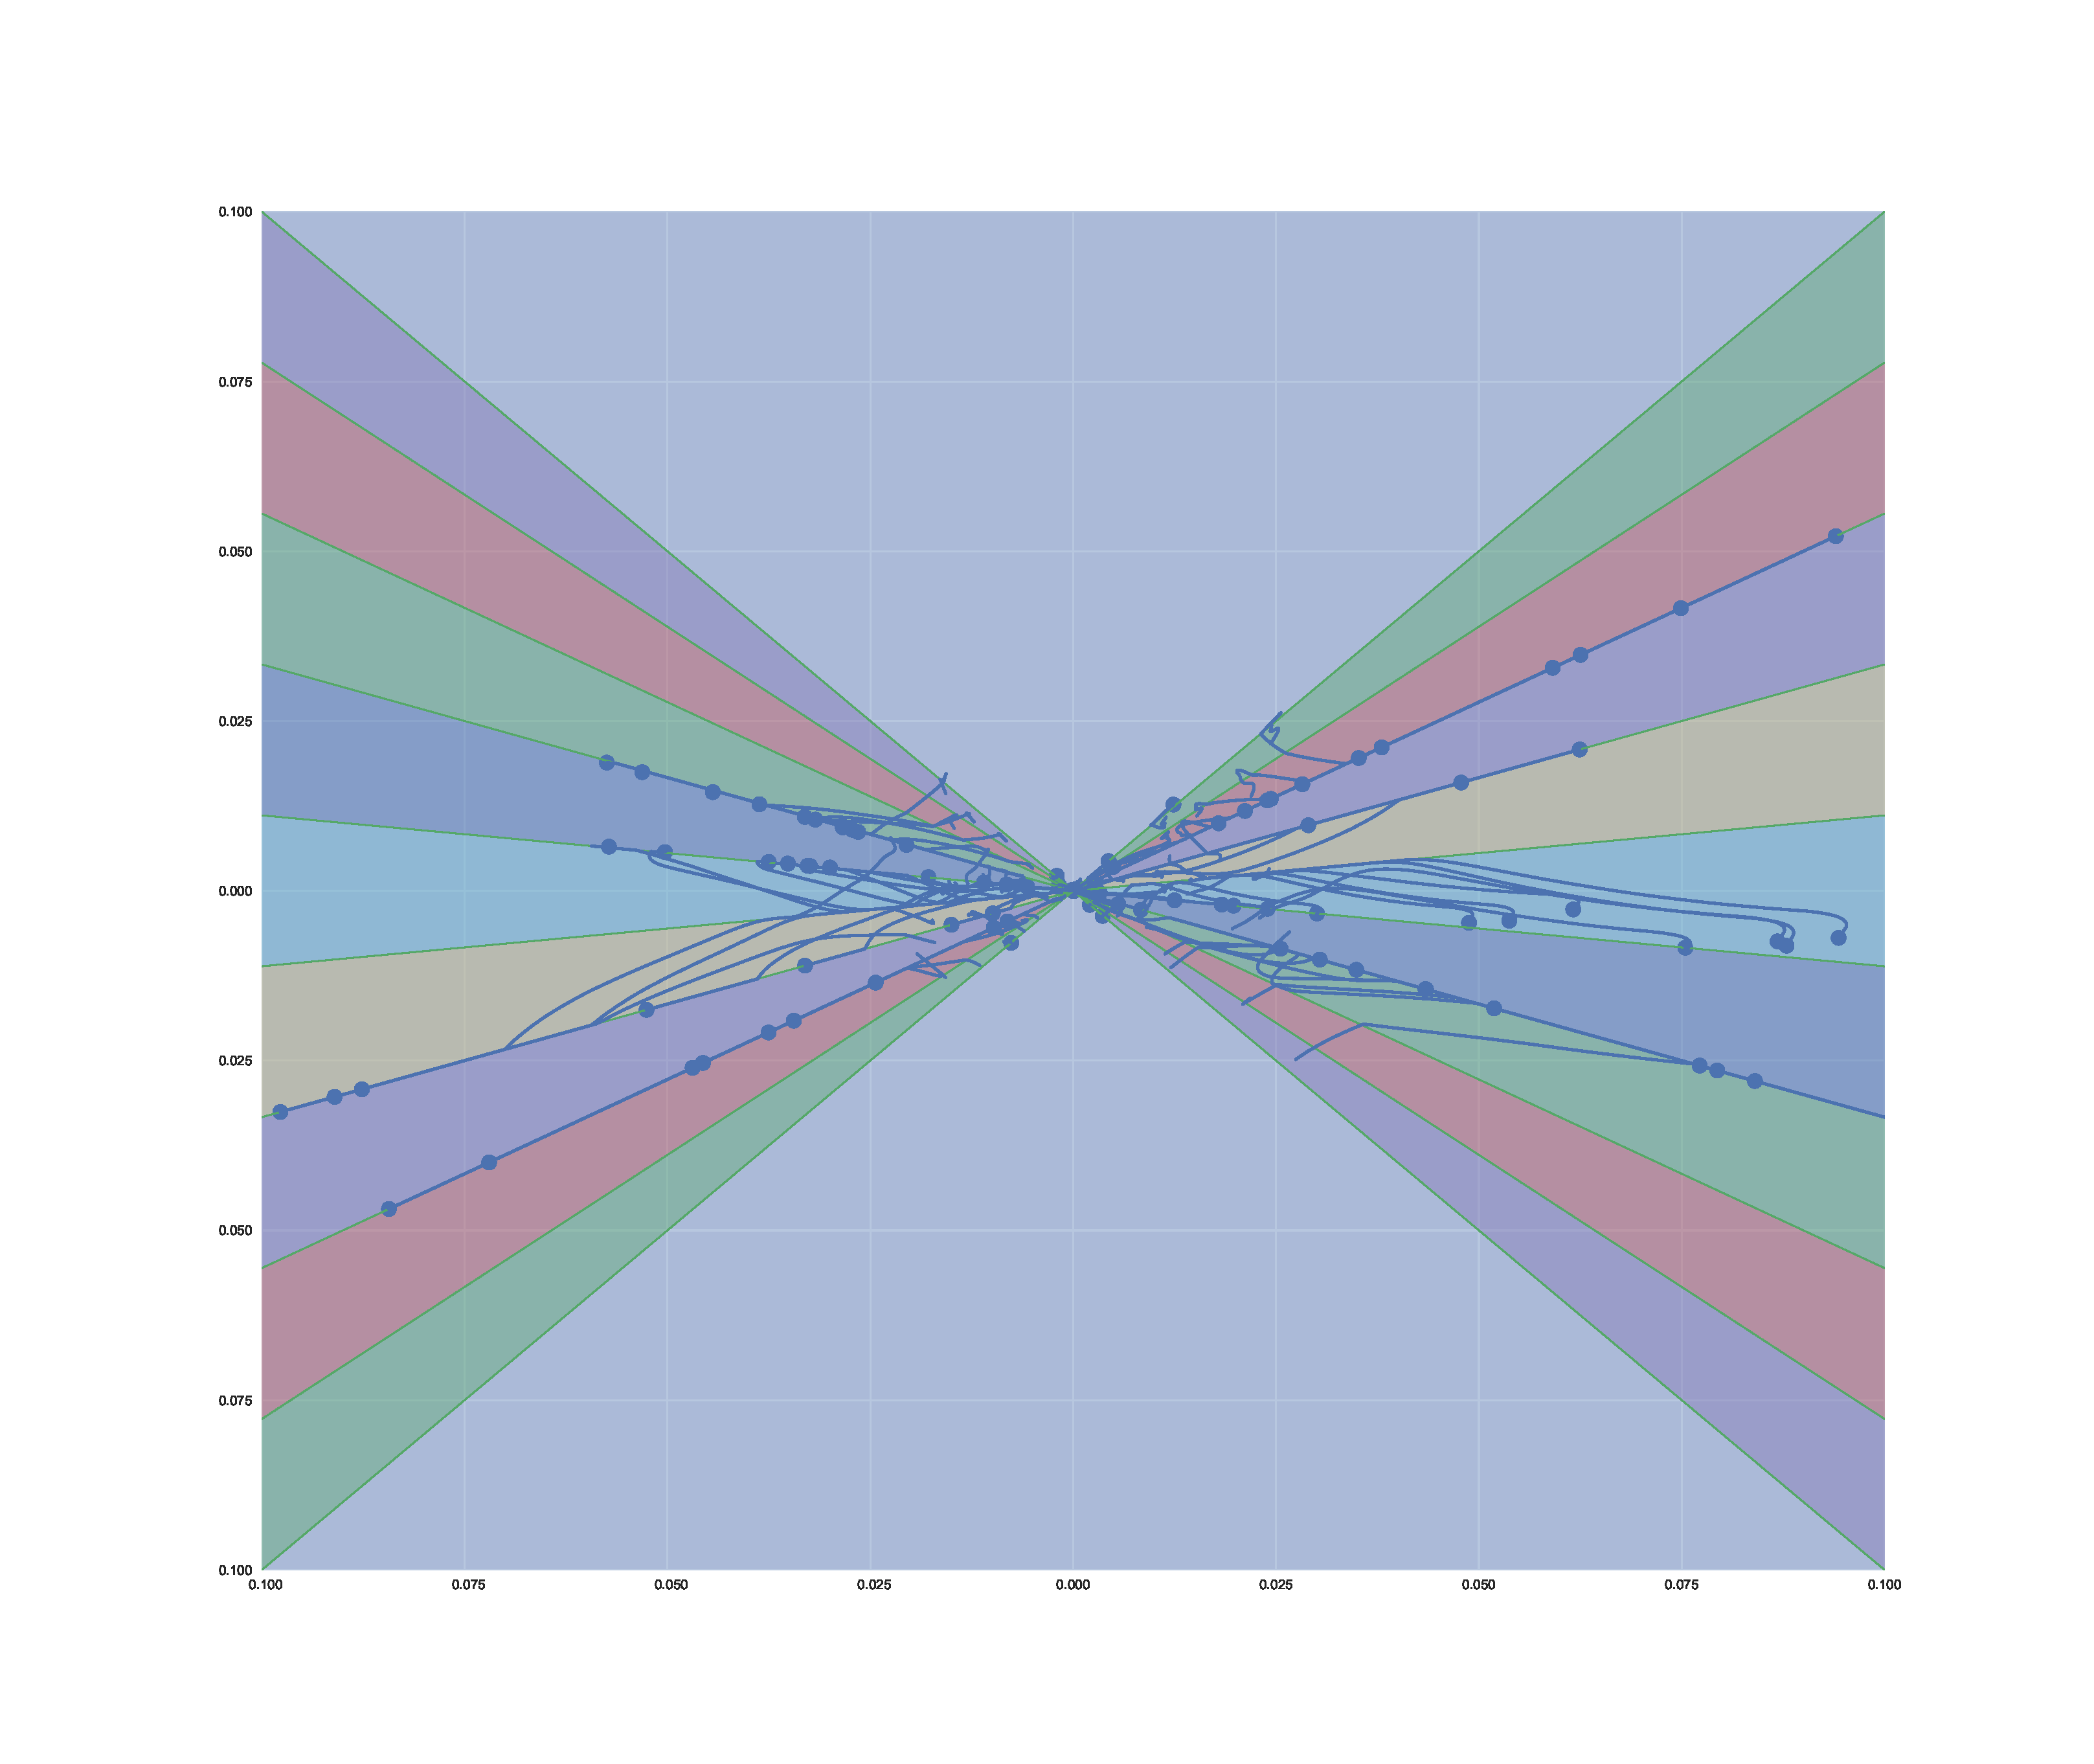
\includegraphics[width=\linewidth]{figures/neuron_trajectories.pdf}
    \endminipage
    \caption{Evolution of neurons in the tangential regime while fitting a square wave with 1000 neurons. The left image shows the trained network on and sample points. The middle image shows the distribution of all neurons at the end of training. The right image shows trajectories for a random sample of 100 neurons. Observe how in this regime, neurons concentrate on certain samples. The trajectories in this case get stuck at the sample boundary.}
    \label{fig:tangential_trajectories}
\end{figure}


\begin{figure}
    \centering
    \minipage{0.33\textwidth}
    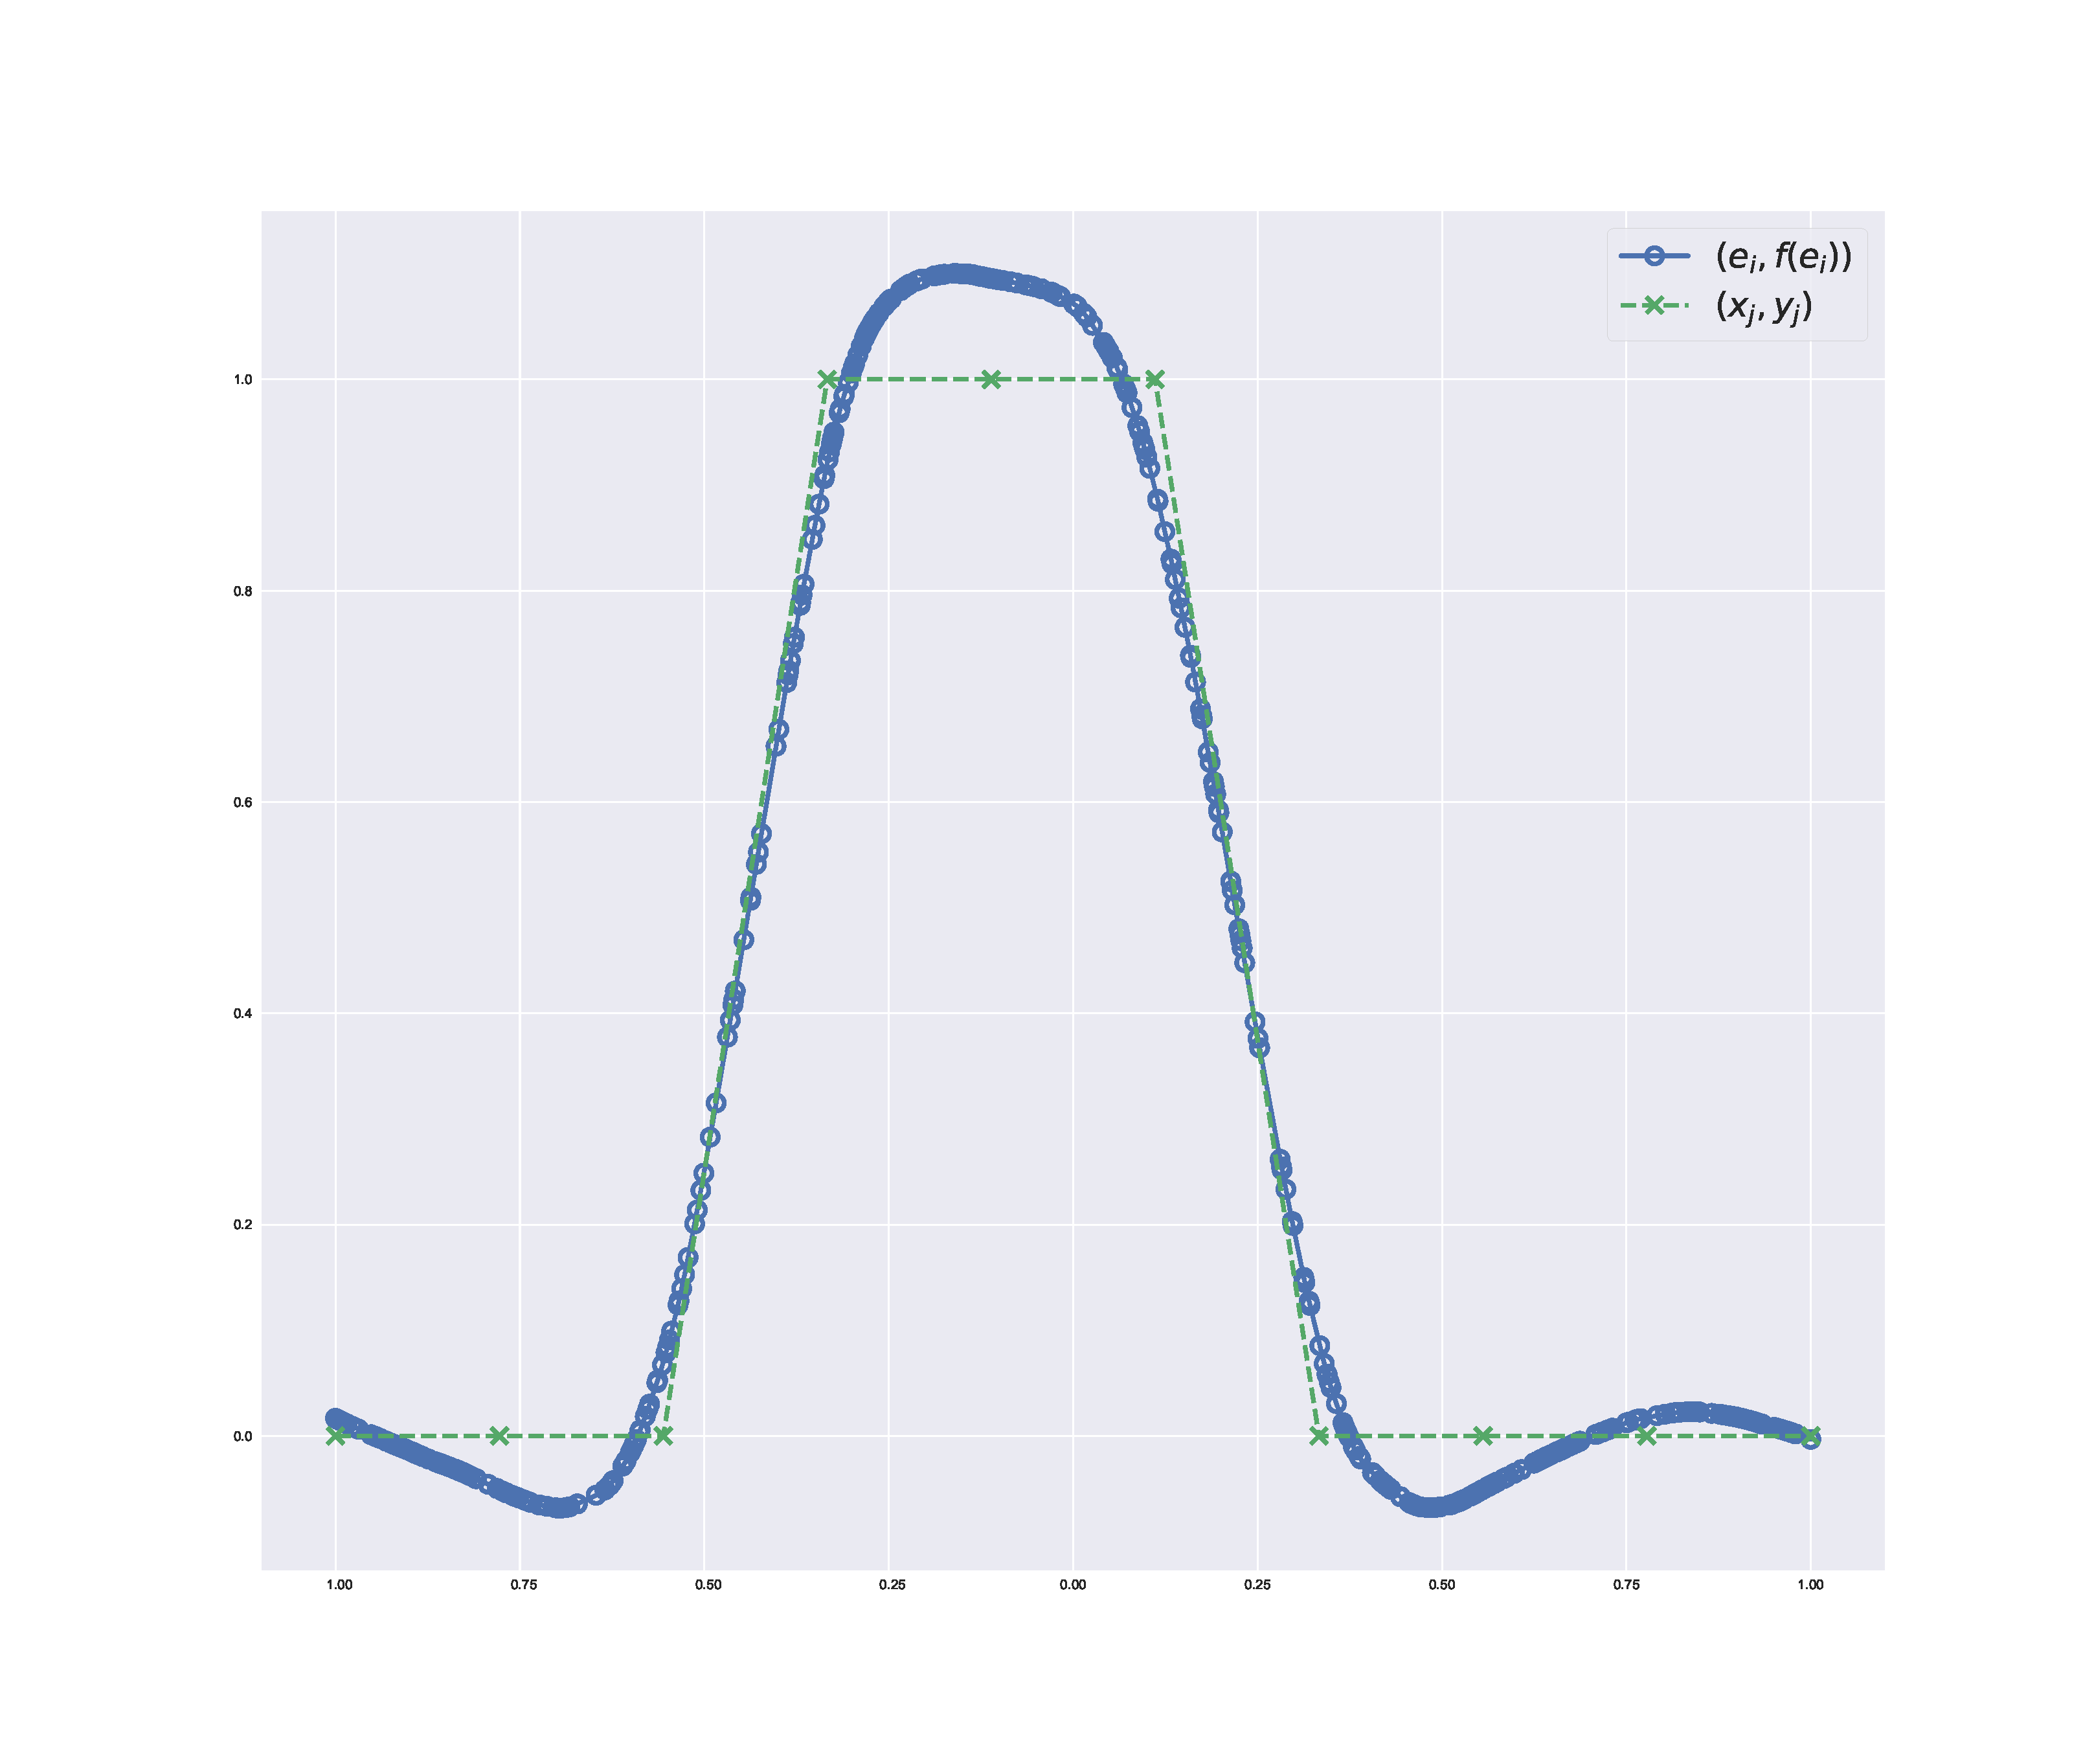
\includegraphics[width=\linewidth]{figures/radial_trajectories_recon.pdf}
    \endminipage\hfill
    \minipage{0.33\textwidth}
    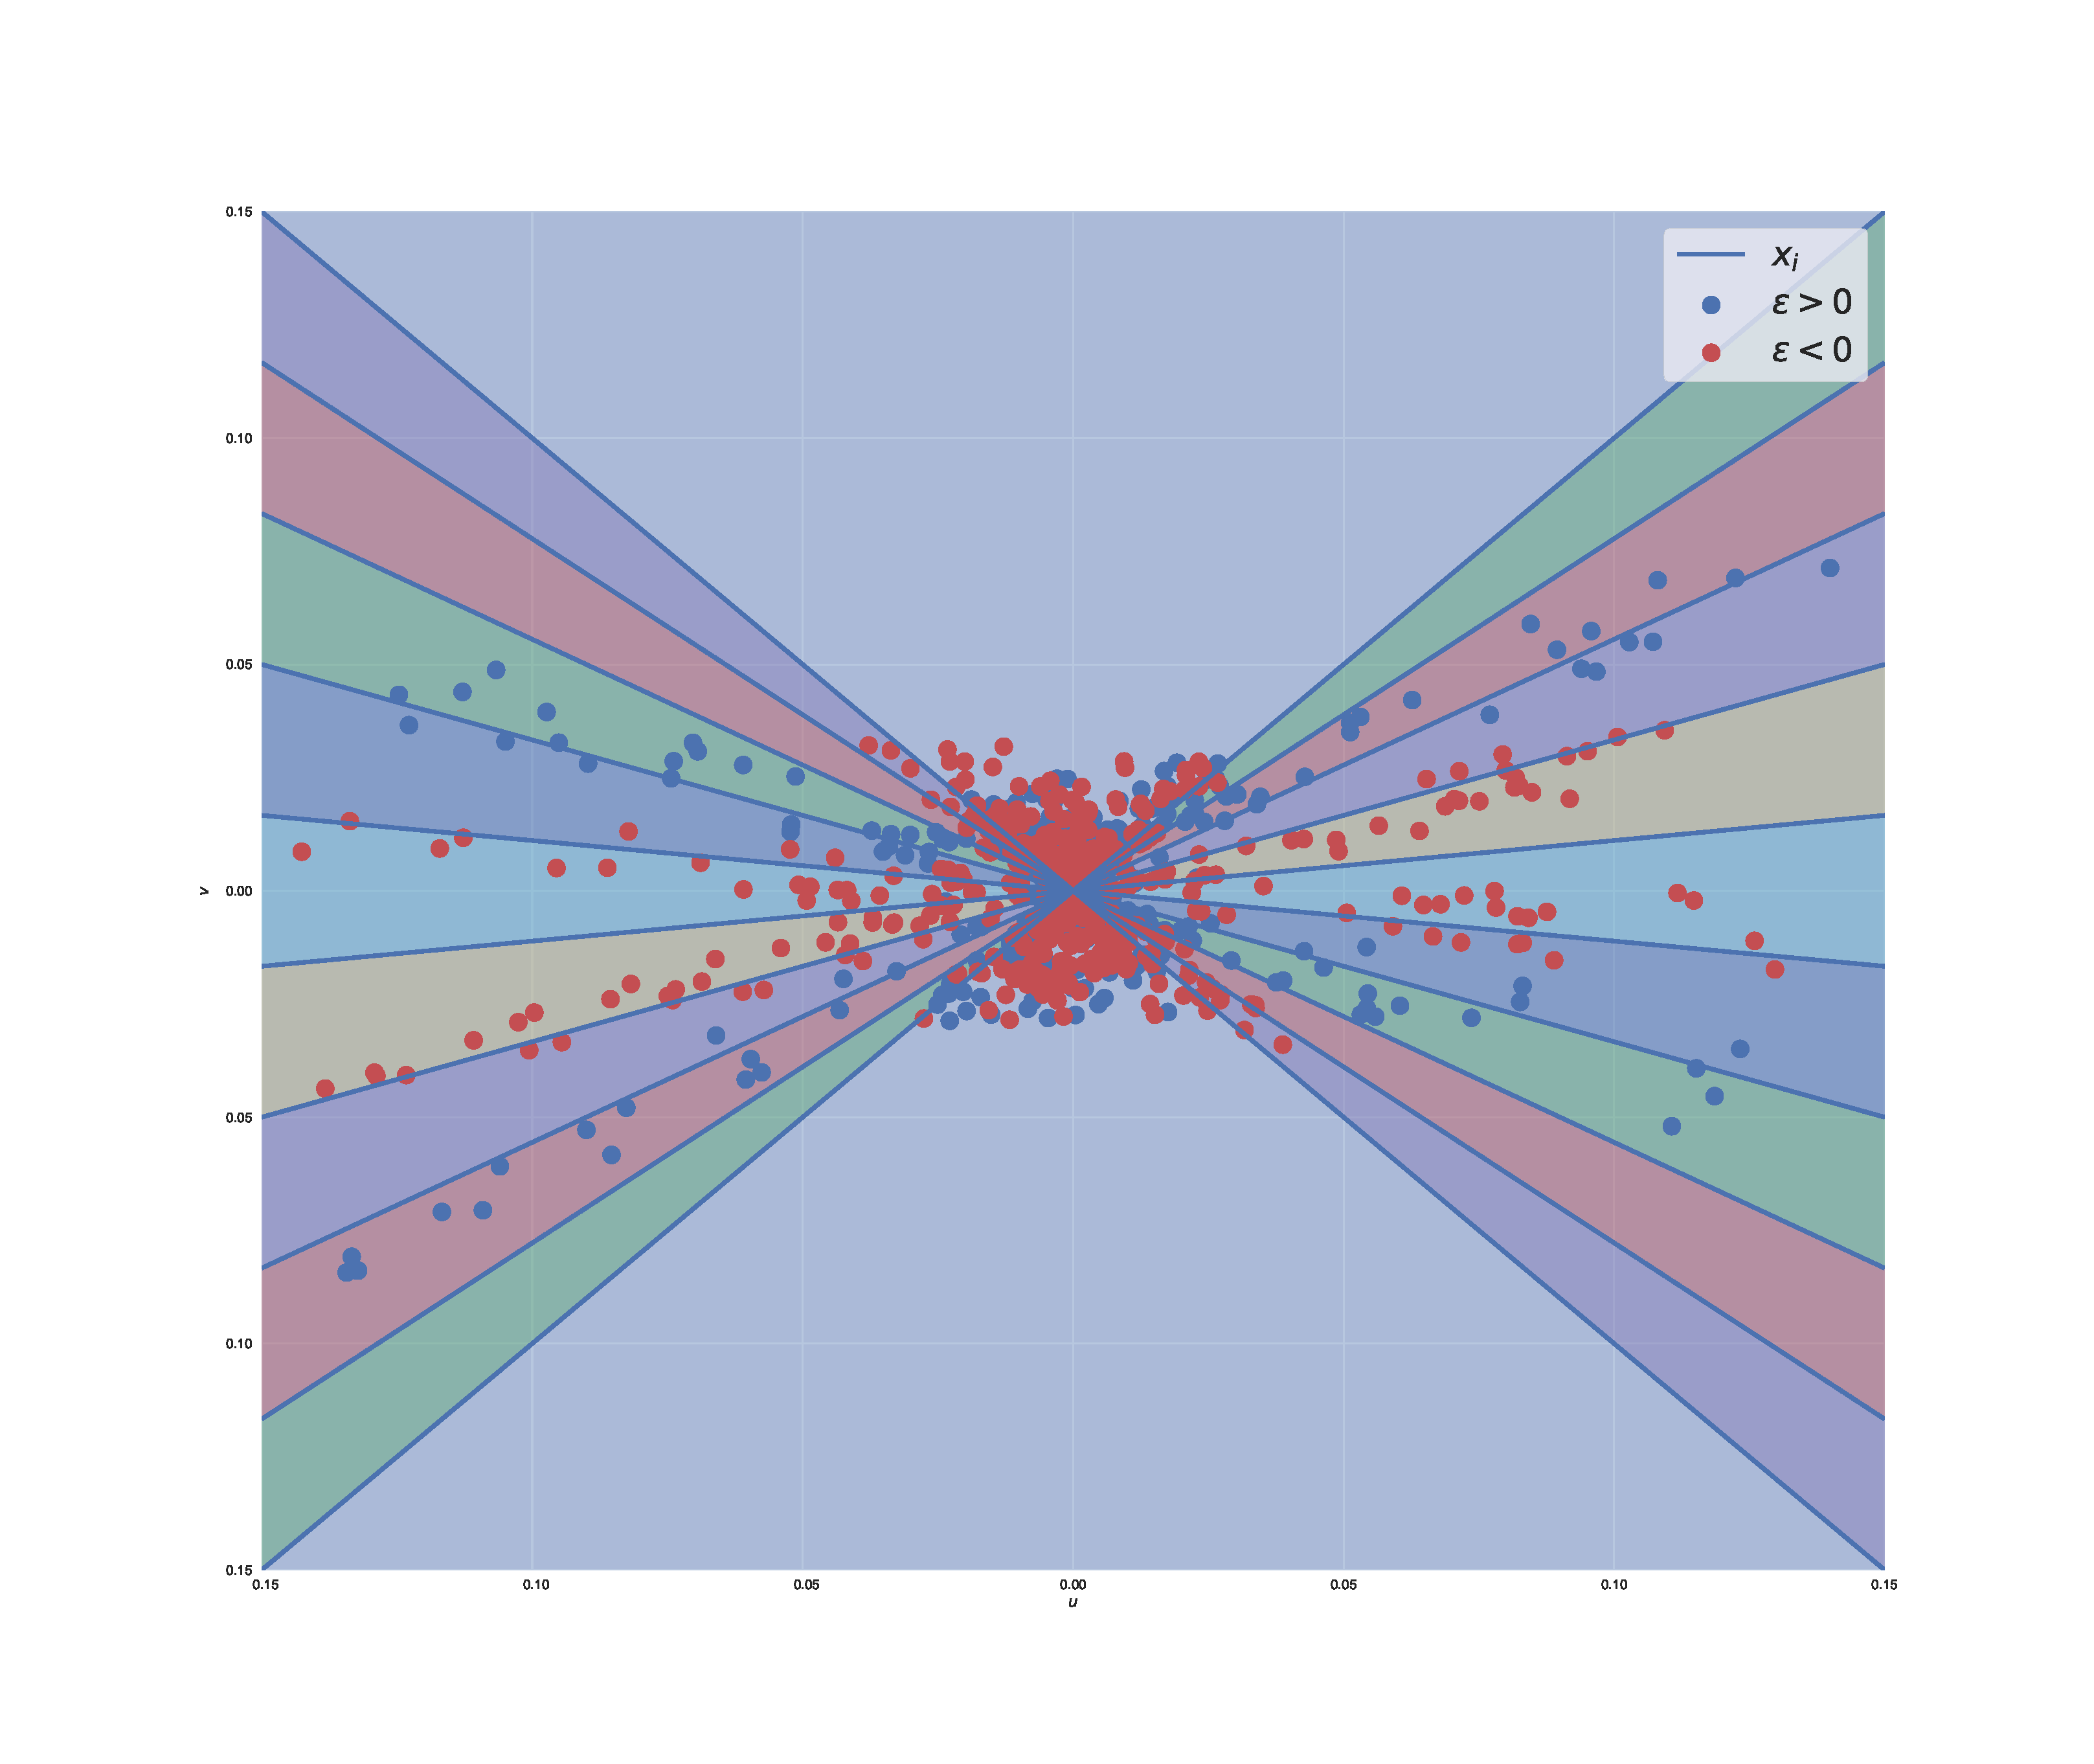
\includegraphics[width=\linewidth]{figures/radial_trajectories_phase.pdf}
    \endminipage\hfill
    \minipage{0.33\textwidth}
    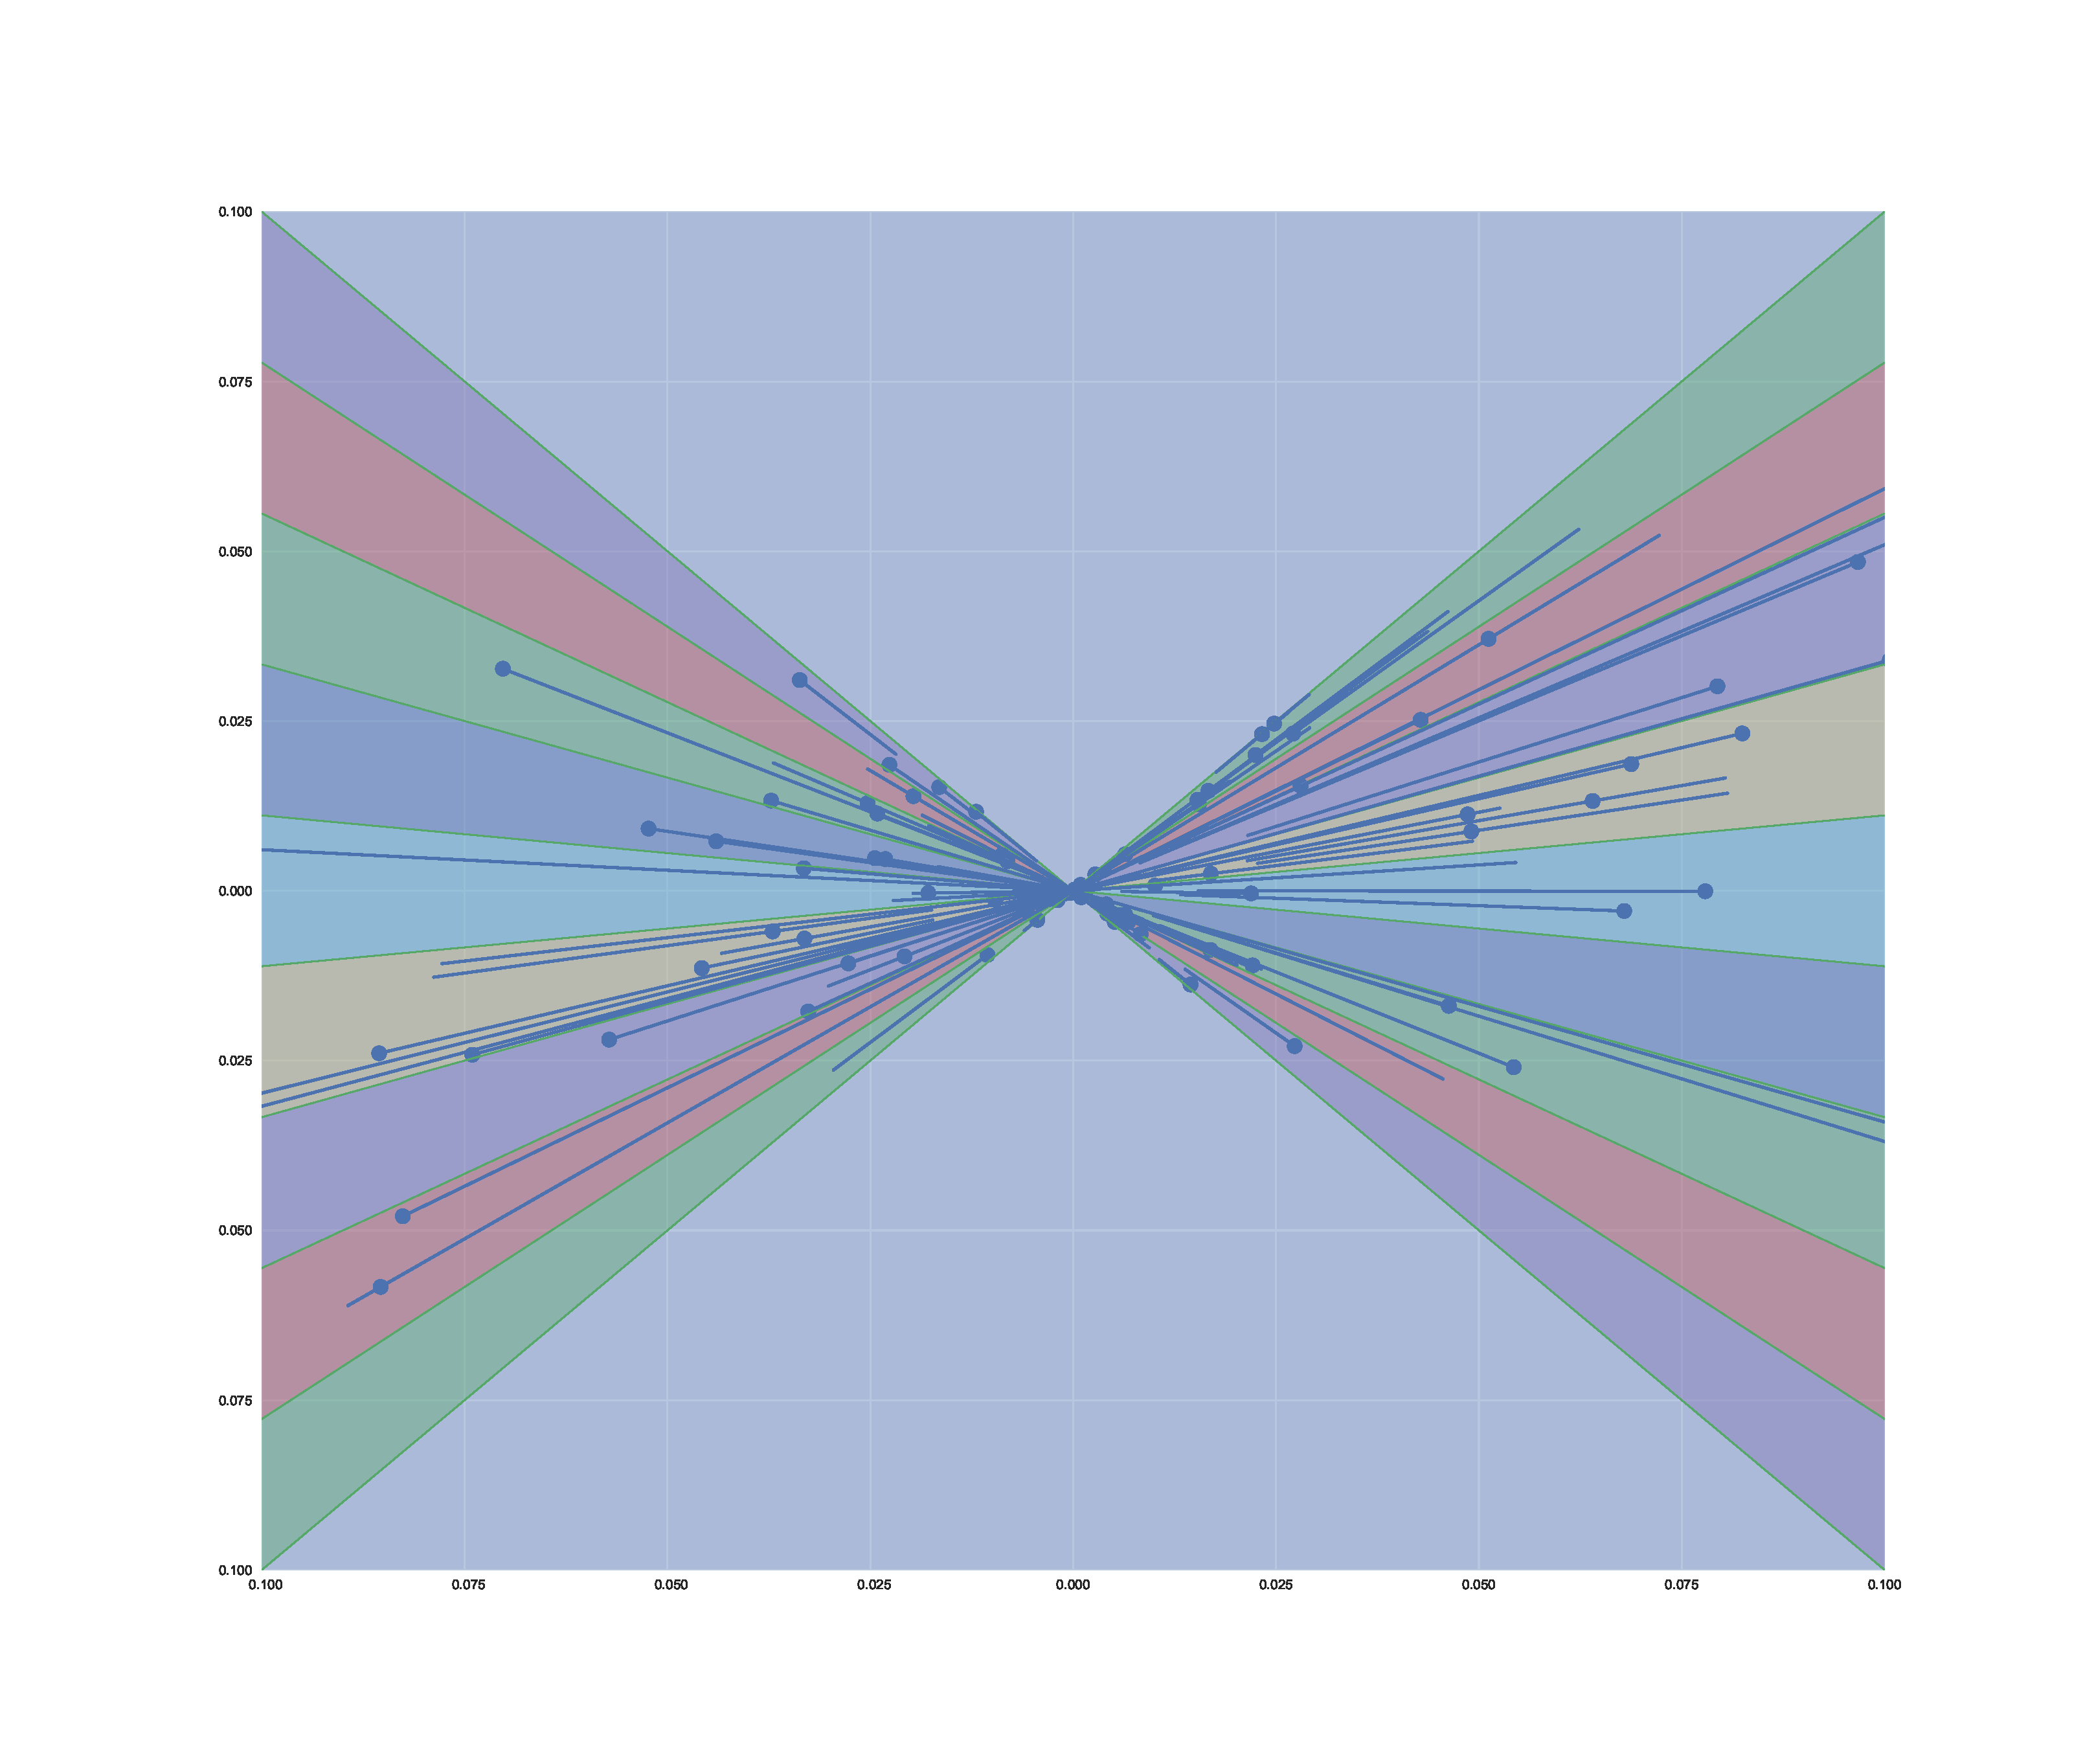
\includegraphics[width=\linewidth]{figures/radial_trajectories.pdf}
    \endminipage
    \caption{Evolution of neurons in the radial regime while fitting a square wave with 1000 neurons. The left image shows the trained network on and sample points. The middle image shows the distribution of all neurons at the end of training. The right image shows trajectories for a random sample of 100 neurons.}
    \label{fig:radial_trajectores}
\end{figure}





\section{Global Training Dynamics}
% The invariants $\delta_i$ allow us to present a concrete framework for understanding the global dynamics of neurons in terms of their initialization. We can understand the global dynamics of neural networks in terms of two regimes corresponding to eigenvectors of $M_\delta$ in the previous section: \emph{Radial training} and \emph{Tangential training}. 

In this section, we consider the extreme cases of initialization: $\delta \ll -\|\xi\|$ (radial dynamics) and $\delta \gg \|\xi\|$ (tangential dynamics). This corresponds to training only the bottom and only the top layer of the network, respectively. 

% We show that lazy training occurs when $\delta \ll 0$ (radial motion in the reduced parameters). We demonstrate that in this regime, the network is biased towards ``smooth'' solutions. At the other end of the spectrum \cite{maennel2018gradient} observe that small initializations lead to a quantization effect of the weight vectors independent of the size of the network. This phenomenon occurs more prominently as $\delta$ grows larger. Furthermore, we describe precisely where the the weight vectors concentrate in terms of the input samples. We also note that the samples at which neurons concentrate are not fixed, but are dynamical quantities which depend on the activation pattern and on the residuals.

% We note that scaling the gradient flow is equivalent to scaling the distributions from which the initial parameters, $\theta$ are sampled, thus we can control the value of $\delta$ by either rescaling the gradient flow or changing the initial distribution of $\theta$.


\subsection{Radial Training}

\note{We should say that radial training is what happens with the standard initialization using pytorch}

In pure radial regime, we are only learning the outer layer parameters and leaving the inner parameters fixed. This corresponds to \emph{kernel learning}~\note{Cite someone}. In the overparameterized setting, we wish to solve

\begin{equation}\label{eq:lsq_overparameterized}
\begin{gathered} 
    \text{minimize } ||c||^2\\
    \text{subject to } M_x(a, b) c = y
\end{gathered}
\end{equation}

which is strictly convex with convex constraints. Writing $M = M_x(a,b)$, we have that solution to \eqref{eq:lsq_overparameterized} is given by $c = M^T (M M^T)^{-1} y$. We define the kernel

\begin{equation}
    K_{(a,b)}(x,x') = \sum_{i=1}^m [a_i x + b_i]_+[a_i x' + b_i]_+
\end{equation}


The optimized function is given by

\begin{equation}
    f(x) = \sum_{j=1}^s v_j K(x_j, x)
\end{equation}


where $v = K(x_i,x_j)^{-1} y$. Of course, this closed form solution only corresponds to the point of convergence of the gradient flow only if $c(0) = 0$. The more general dynamics of the flow can be similarly derived in terms of the kernel $K$ (see Appendix). Furthermore, it is known in this setting that early stopping for
gradient descent will act as a regularizes as these eigenfunctions of $K$ typically correspond to lower frequency features of the function being fit \note{cite}.







\paragraph{Infinite width limit}
% We analyze the behavior of the \emph{limit kernel} as the number of weights $m \rightarrow \infty$ in the radial regime. We show that the overparameterized least squares problem in this setting minimizes curvature. Furthermore, for 1D functions, the network functions are natural cubic spines. 
In the infinite width ($m = \infty)$ limit, the parameters, $\theta$ become densities $\theta(s) = (a(s), b(s), c(s))$. Assuming that $s \in [k_1, k_2], x \in [k_1, k_2]$, then we can write the function $f$ as

\begin{equation}
    f(x) = \int_{k_1}^{k_2} c(s) [a(s) x + b(s)]_+ ds
\end{equation}

and the least squares problem becomes
\begin{equation}
    \begin{gathered}
    \text{minimize } ||c(s)||^2\\
    \text{subject to } \int_{k_1}^{k_2} c(s) [a(s)x_i + b(s)]_+ ds = y_i
    \end{gathered}
\end{equation}

\begin{lemma}\label{le:curvature}
The second derivative of $f(x)$ is the parameter density $c(s)$. i.e. 
\begin{equation*}\partial_x^2 f(x) = c(s)\end{equation*}
\end{lemma}
\begin{proof}
\todo{TODO}
\end{proof}

Thus, the quantity $||c(s)||^2 = ||\partial_x^2 f(x)||^2$ being minimized is the \emph{curvature}. Thus, we can view the radial regime as an implicit bias towards ``smooth'' functions.



For 1D functions with knots initialized from a uniform distribution, we give an exact equation for the limit kernel. 

\begin{lemma}\label{le:cubic_spline}
Assume that the knots $e(s) =\ -\frac{b(s)}{a(s)} ~ U(k_1, k_2)$, then the inifinite width kernel, $K(x, y)$ is a cubic polynomial in $x$ and $y$
\end{lemma}
\begin{proof}

We can rewrite the kernel,
\begin{equation}
    K(x, y) = \int_{k_1}^{k_2} [a(s)x + b(s)]_+ [a(s)y + b(s)]_+ ds
\end{equation}

in terms of the knots $e(s)$

\begin{equation}
    K(x, y) = \int_{k_1}^{k_2} \tau(x, s) \tau(y, s) a(s)^2 (x - e(s)) (y - e(s)) ds
\end{equation}

where $\tau(x, s) = \mathds{1}[a(s)x + b(s) \geq 0]$. $a(s)$. Sicne the knots $e(s) = -\frac{b(s)}{a(s)}$ are uniformly distributed, we can write $e(s) = s$ which implies $-b(s) = s a(s)$. In this case, we can assume without loss of generality that $v(s) = -s$ and $u(s) = 1$. We then rewrite the kernel

\begin{equation}
    \begin{aligned}
    K(x, y) &= \int_{k_1}^{k_2} \tau(x, s) \tau(y, s) (x - s) (y - s) ds\\
            &= \int_{k_1}^{\min(x, y)} (x - s) (y - s) ds\\ 
            &= s xy - \frac{1}{2} s^2 (x + y) - \frac{1}{3} s^3 \bigg\rvert_{k_1}^{\min(x, y)}
    \end{aligned}
\end{equation}

which is a cubic function in $x$ and $y$.
\end{proof}

Recall that for full rank $M_x(a,b)$, the function $f(x)$ interpolates the samples, $x_i$. Thus, a corollary to Lemmas \ref{le:curvature} and \ref{le:cubic_spline} is that for uniform knot initialization, 1D neural network functions are cubic splines interpolating the samples. Figure~\ref{fig:cubic_splines} shows the convergence to a cubic spline as the number of neurons grows large. \note{We need to cite the paper on linear splines here.} 

\begin{figure}\label{fig:cubic_splines}
    \centering
    \minipage{0.33\textwidth}
    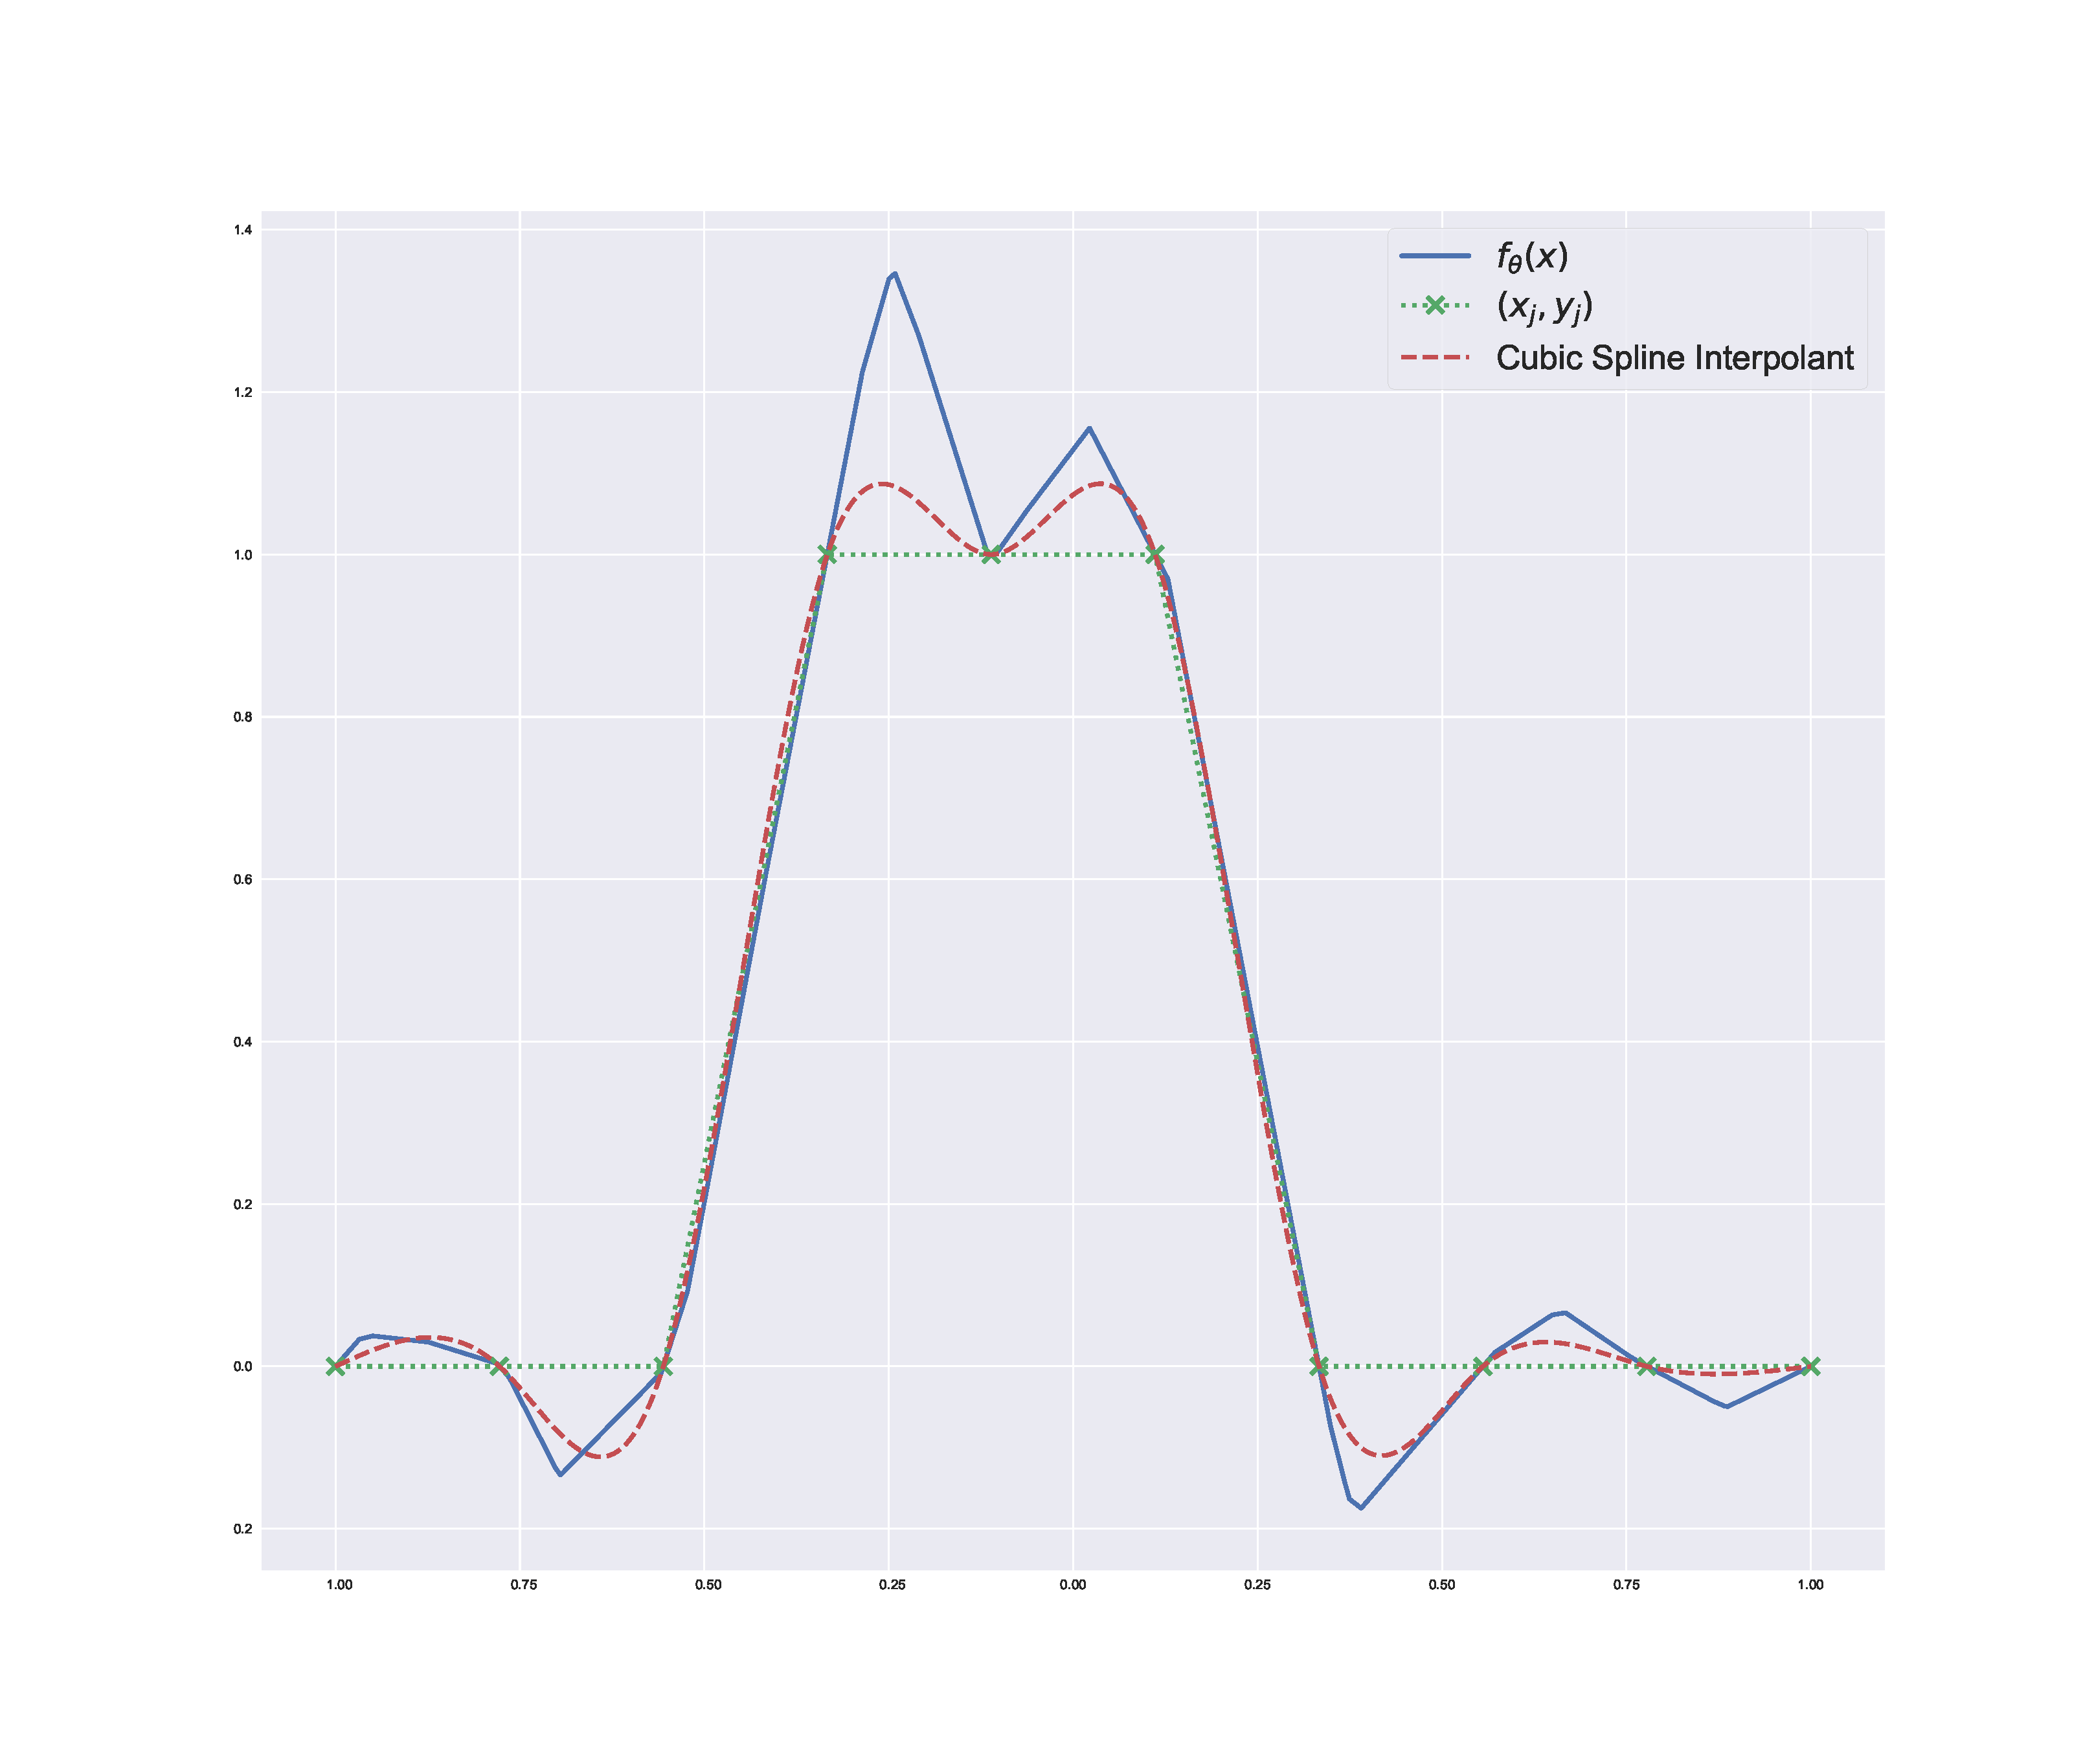
\includegraphics[width=\linewidth]{figures/cubic_spline100.pdf}
    \endminipage\hfill
    \minipage{0.33\textwidth}
    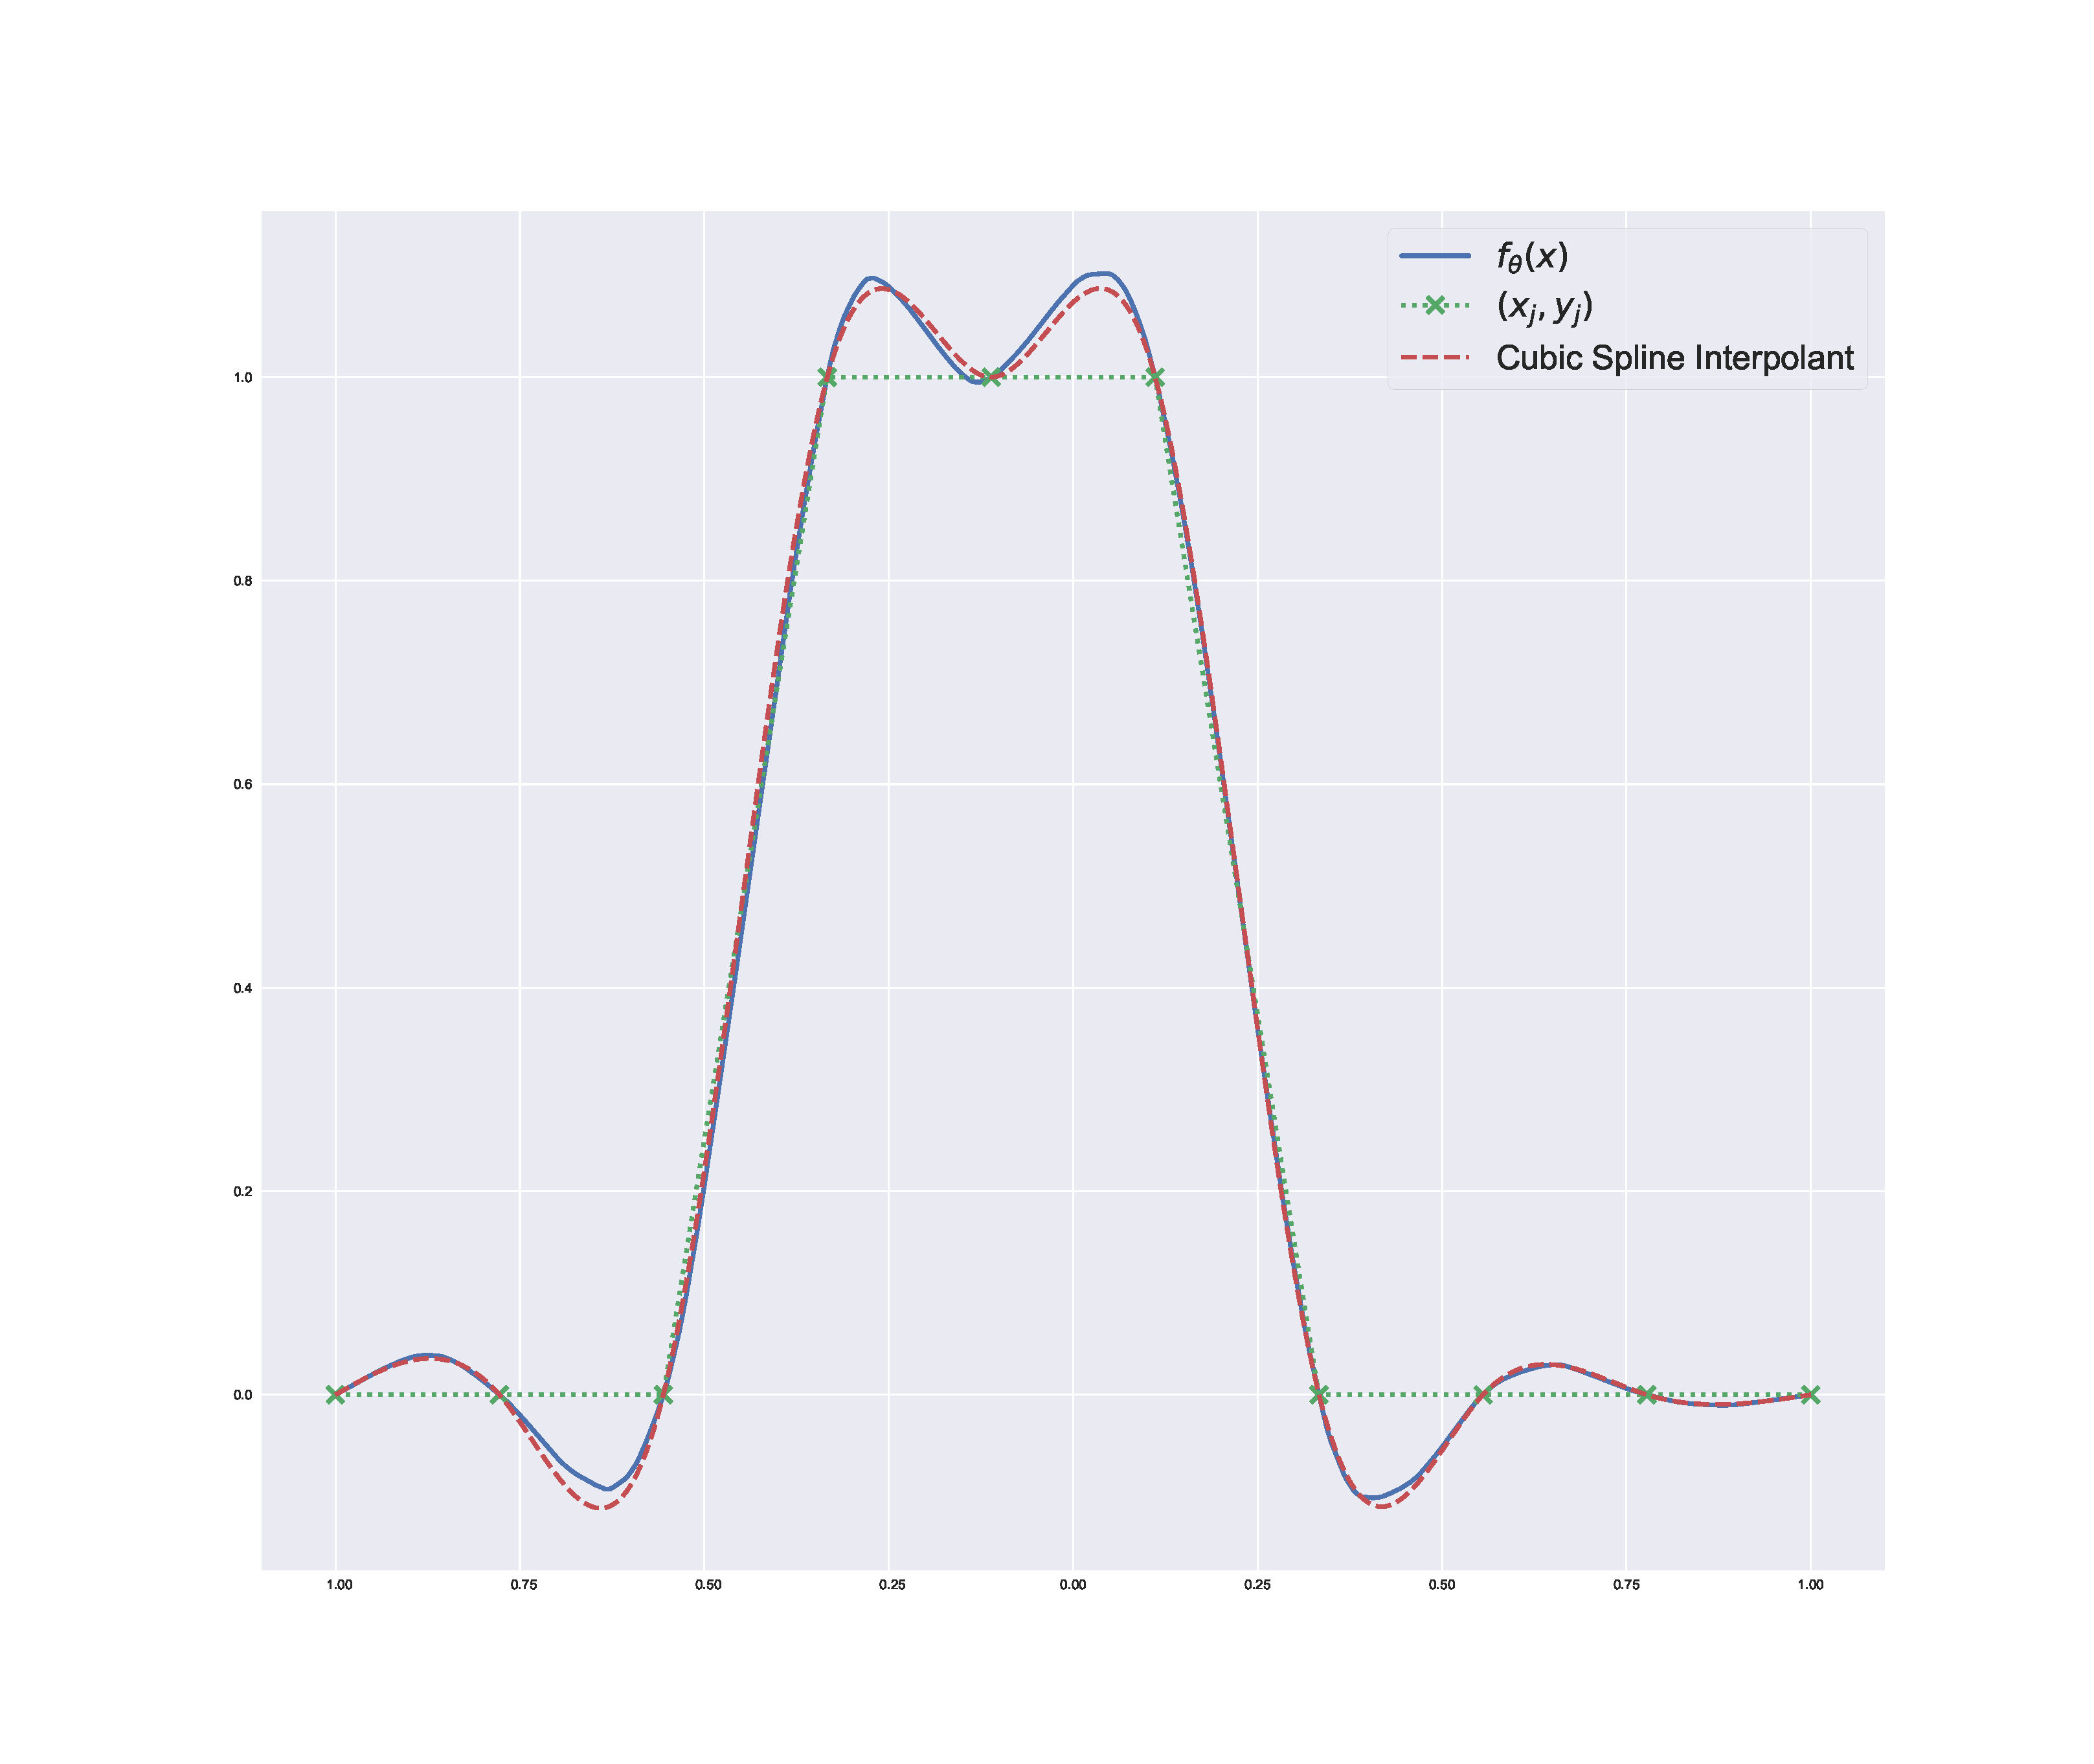
\includegraphics[width=\linewidth]{figures/cubic_spline_1k.pdf}
    \endminipage\hfill
    \minipage{0.33\textwidth}
    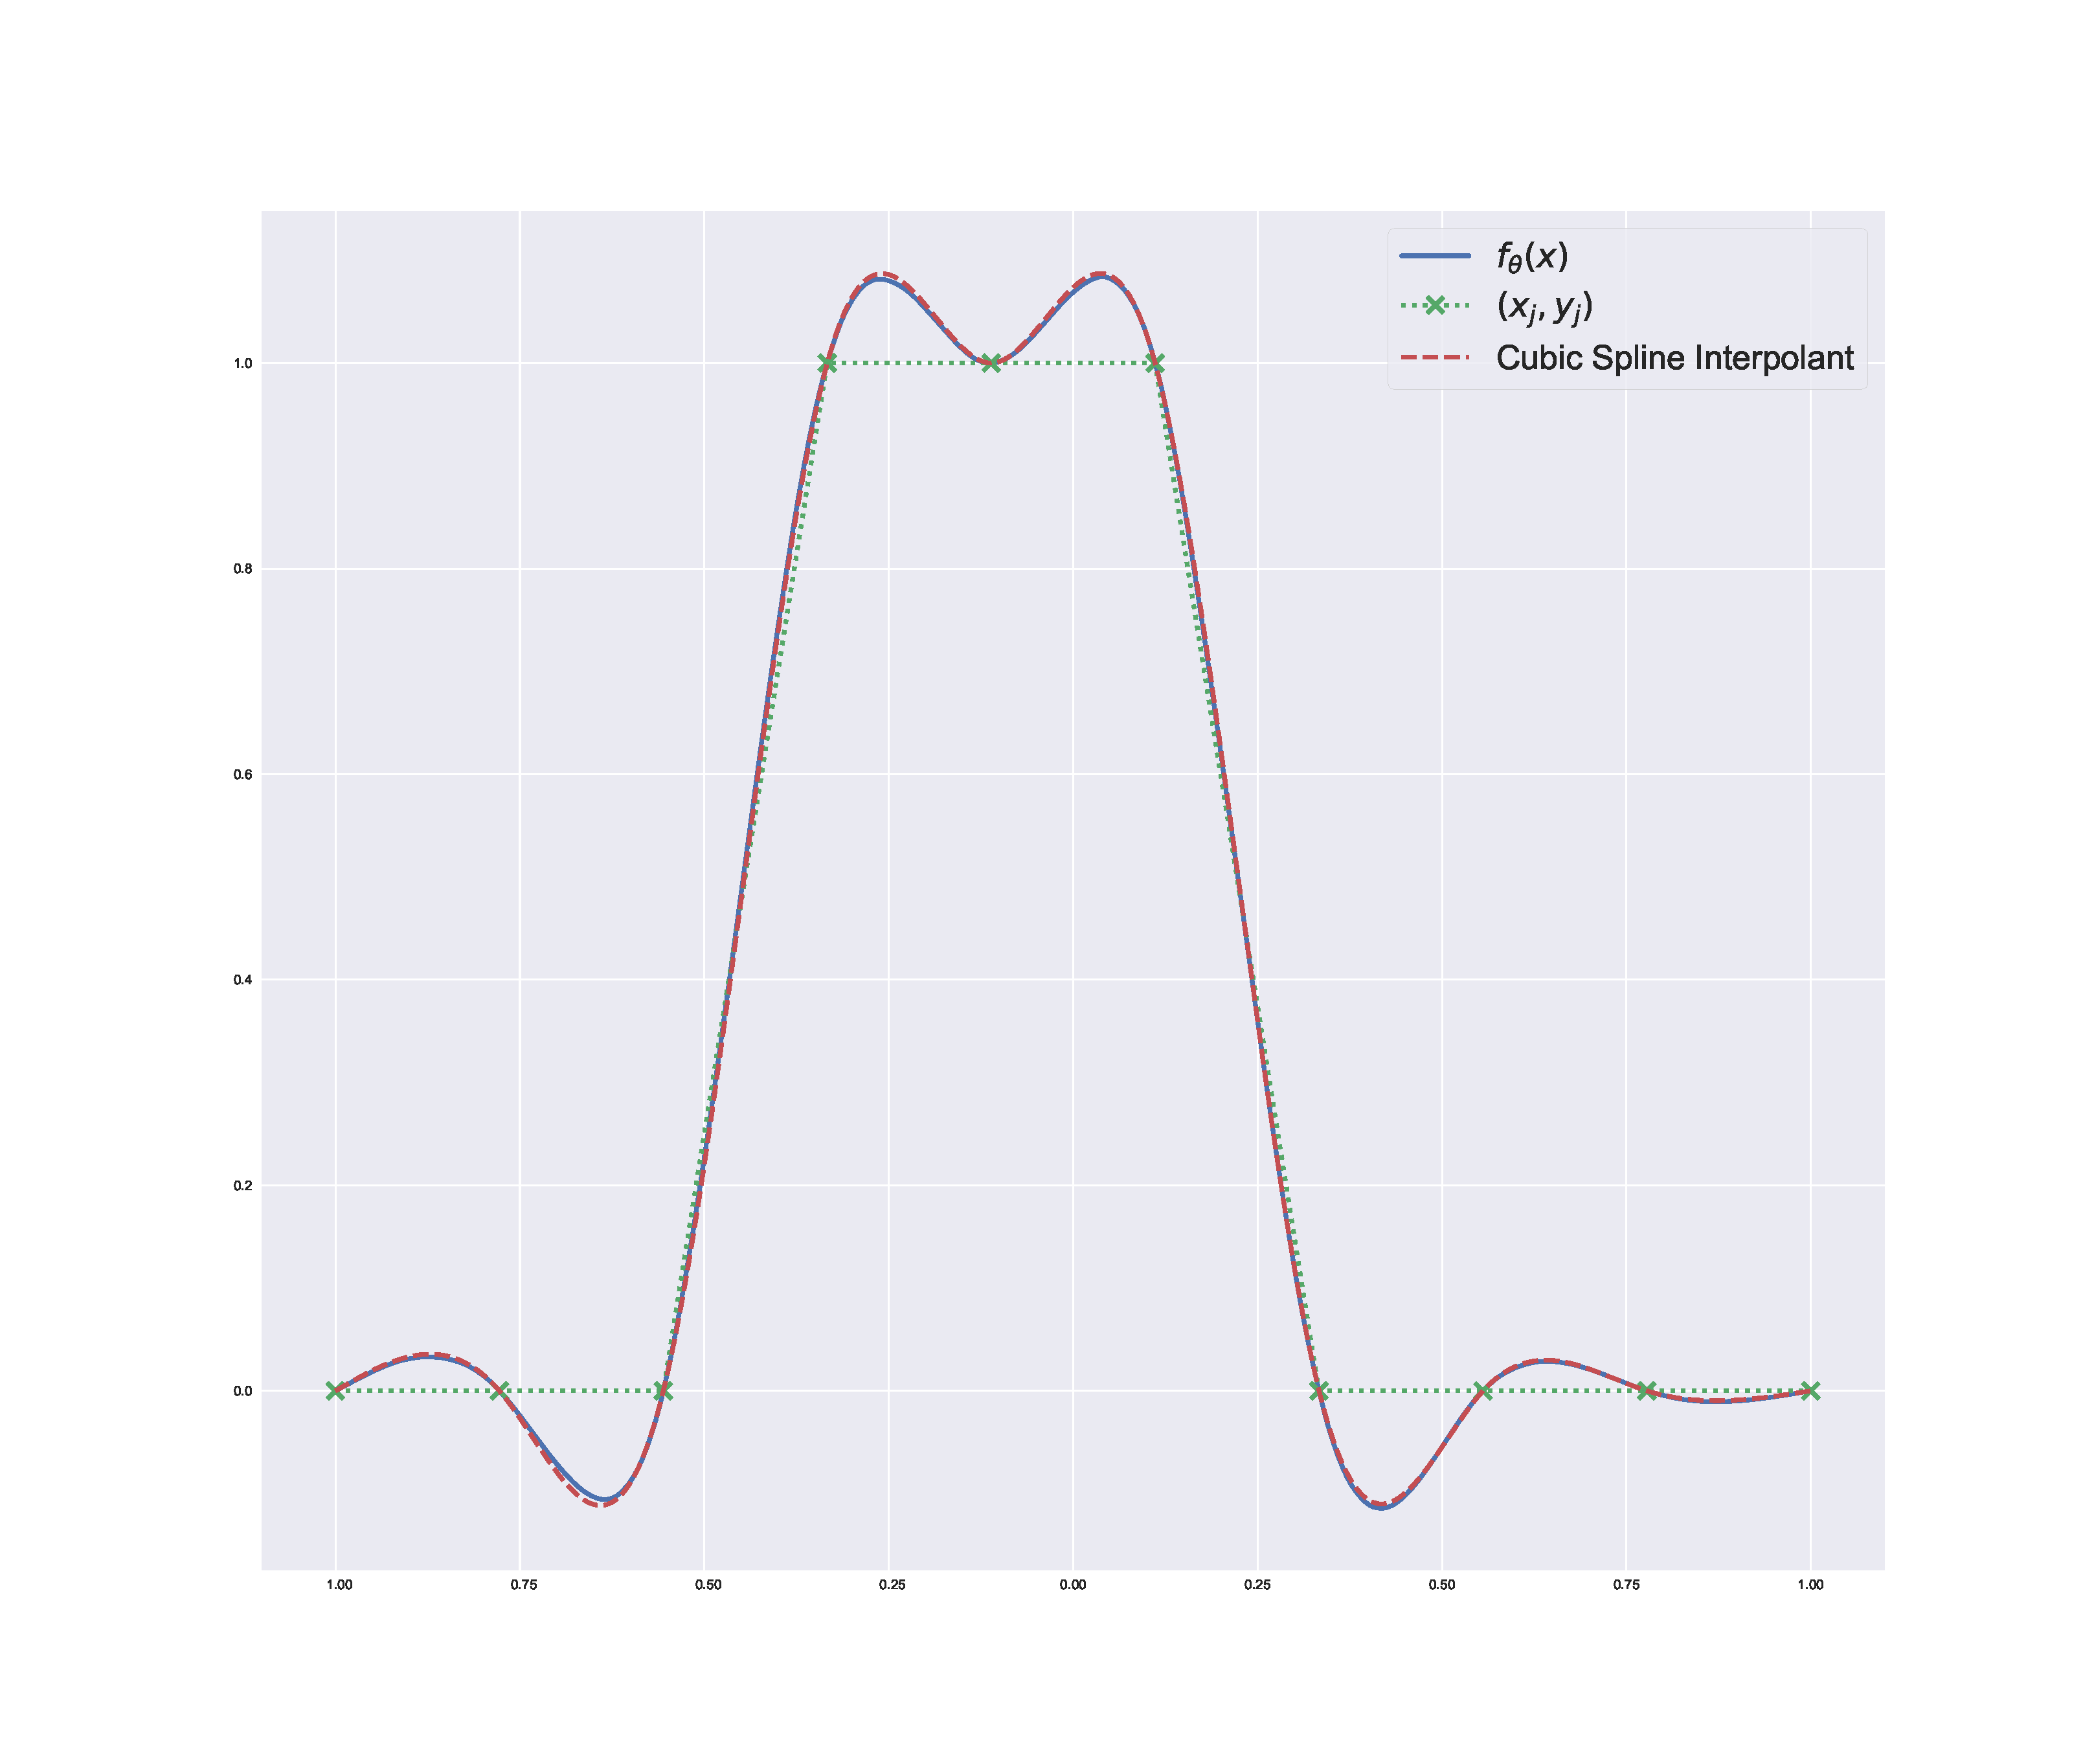
\includegraphics[width=\linewidth]{figures/cubic_spline_10k.pdf}
    \endminipage
    \caption{Regression in the purely tangential regime ($\delta = -\infty$) using varying knots. We observe that as the number of knots increases, the function, $f_\theta$ converges to a cubic spline interpolant with $\partial_x^2 = 0$ on the boundary.}
    \label{fig:radial_trajectores}
\end{figure}



















\subsection{Tangential Training, $\delta \gg \|\xi\|$}


\note{Use interesting?}

Recall that Lemma~\ref{le:pw_continuous} states that the gradient field $\nabla \tilde{L}$ is piecewise continuous. An important consequence of this result is that the gradient field could point in opposite directions on the boundary of a sample (\todo{Figure \ref{fig:todo}}). In this case, a neuron could get stuck along the boundary for that sample and only be able to move radially. We call the samples at which neurons get stuck \emph{attractive}. The existence of attractive samples leads to neurons piling up at samples, biasing the functions $f(x)$ to be piecewise linear with a small number of pieces.

We now give a precise condition for when a sample is attractive. We also show that the set of attractive samples is a dynamical quantity which depends only on the activation.

Recall that in the reduced parameter space, a sample $x_i$ corresponds to a line in the $(u, v)$ plane. The sample $x_i$ is \emph{attractive} if the loss gradient in the reduced parameters $\nabla \tilde{L}$ points in opposite directions on either side of this line. 

Formally, we can express attractiveness as a condition on the time derivative of the knots $e_i(t)$. 

\begin{equation}\label{eq:moving_knots}
\partial_t e_i(t) = \frac{-a_i \partial b_i + b_i \partial a_i}{a_i^2} = c_i\frac{- a_i \sum_
{j=1}^s
\tau_{ij} r_j + b_i \sum_
{j=1}^s \tau_{ij} x_j r_j}{a_i^2} = \frac{\sum_{j=1}^s \tau_{ij}c_i(-a_i
+x_j b_i)r_j}{a_i^2}
\end{equation}

\note{Possibly useful to frame attractiveness/interestingness:}
\begin{definition}
Consider a function of the form $h(\bm w) = \sum_{i=1}^s r_i [\langle \bm w,\bm x_i\rangle ]_+$ with $\bm w, \bm x_i \in \RR^2$ and $r_i \in \RR$. We say that $\hat{ \bm w} \in \mathbb S^1$ is a \emph{stable direction} if $\hat{ \bm w} \in \alpha \partial h(\hat {\bm w})$ for some $\alpha > 0$ (perhaps give more intuitive definition/picture?).
\end{definition}

A stable direction can either be on the boundary or on the internal part of a segment. From~\eqref{eq:moving_knots}, we are interested in the stable directions for $h((a_i,b_i)) = \epsilon_i \sum_{i=1}^s r_j [(-a_i + x_jb_j)]_+$. Stable directions on the boundaries are ``interesting points''.


\note{Think about how to present this}

Assume that the samples $x_1 < x_2 < \ldots < x_s$ are ordered and suppose that the knot $e_i$ lies on the sample $x_k$, i.e. $e_i(t) = x_k$. Denoting $r = (r_j(\theta))_{j=1}^s$ as the vector of residuals, we have that a the sample $x_k$ is attractive if

\begin{equation}
\begin{aligned}
    &\sum_{j=1}^{k-1} (1+x_j x_k) r_j \lessgtr 0 \quad \mbox{ and } \qquad \sum_{j=1}^k (1+x_j x_k) r_j \gtrless 0, \quad \mbox{ or }\\
    &\sum_{j=k}^s (1+x_j x_k) r_j \gtrless 0 \quad \mbox{ and } \qquad \sum_{j=k+1}^{s} (1+x_j x_k) r_j \lessgtr 0.\\
\end{aligned}
\end{equation}

If $z_j = (1,x_j) r_j$, we can rewrite this as

\begin{equation}
\begin{aligned}\label{eq:attractor_cond}
    &\sum_{j=1}^{k-1} \langle z_k , z_j \rangle < 0 \quad \mbox{ and } \qquad \sum_{j=1}^{k} \langle z_k, z_j \rangle > 0, \quad \mbox{ or }\\
    &\sum_{j=k}^{s} \langle z_k , z_j \rangle > 0 \quad \mbox{ and } \qquad \sum_{j=k+1}^{s} \langle z_k, z_j \rangle < 0.\\
\end{aligned}
\end{equation}


This can be written in terms of the Gram matrix $Z_{ij} = (\langle z_i, z_j\rangle)$.

\paragraph{Dynamics of Attractive Samples}

The attractiveness condition \eqref{eq:attractor_cond} is a dynamic quantity depending on the residuals $r(\theta)$ as well as the samples, $x$. A sample can only change from attractive to unattractive or vice-versa when the activation matrix $\tau$ changes.

\begin{lemma}
If the truth value of the condition \eqref{eq:attractor_cond} changes at time $t$, then the activation matrix, $\tau$ must also change at time $t$.
\end{lemma}
\begin{proof}
\todo{TODO}
\end{proof}

Qualitatively, a sample is attractive when there is a large change in sign between the average residual on one side of the sample and the sample itself. Attractive samples on the ''peaks`` and ``valleys of the of the residual. As with the residual case, low frequency features in the data tend to be fit first with high frequency features being fit later. \todo{Figure~\ref{fig:todo}} shows an example of this behavior.



























\iffalse
\subsection{Old}
% It is easy to verify that the eigenvalue-eigenvector pairs of $K(\xi)$ are
% $(\beta a^2+ \beta b^2 + \alpha c^2, (a,b))$ and $(\alpha c^2, (-b,a))$, which correspond to radial and tangential components of $(u, v)$. From this we deduce that


% \begin{itemize}
%     \item If $\alpha c^2 \ll \beta (a^2 + b^2)$, which means that $\delta <
%     0$, then $\xi_i'(t) \propto (a(t),b(t))$, and the reduced neuron
%     moves~\emph{radially}.
%     \item If $\alpha c^2 \gg \beta (a^2 + b^2)$, which means that $\delta > 0$, then
%     $\xi_i'(t) \propto \nabla^\xi(\xi)_i$, so the reduced neuron follows themaybePres
% \end{itemize}



\paragraph{Node dynamics.}

\begin{equation}
\dot e_i(t) = \frac{-\dot b_i a_i + \dot a_i b_i}{a_i^2} = c_i\frac{- a_i \sum_
{j=1}^s
\tau_{ij} r_j + b_i \sum_
{j=1}^s \tau_{ij} x_j r_j}{a_i^2} = \frac{\sum_{j=1}^s \tau_{ij}c_i(-a_i
+x_j b_i)r_j}{a_i^2}
\end{equation}

If $e_i(t) = x_k$, that is, $-b_i = x_k a_i$, then

\begin{equation}
\dot e_i(t) = -\frac{c_i}{a_i}\sum_{j=1}^s \tau_{ij} (1
+ x_j x_k)r_j
\end{equation}

Assuming $x_1 < \ldots < x_s$, we say that a sample point $x_k$ is \emph{attractive} for a residual vector $r$ if

\begin{equation}
\begin{aligned}
    &\sum_{j=1}^{k-1} (1+x_j x_k) r_j \lessgtr 0 \quad \mbox{ and } \qquad \sum_{j=1}^k (1+x_j x_k) r_j \gtrless 0, \quad \mbox{ or }\\
    &\sum_{j=k}^s (1+x_j x_k) r_j \gtrless 0 \quad \mbox{ and } \qquad \sum_{j=k+1}^{s} (1+x_j x_k) r_j \lessgtr 0.\\
\end{aligned}
\end{equation}

If $z_j = (1,x_j) r_j$, we can rewrite this as

\begin{equation}
\begin{aligned}\label{eq:attractor_cond}
    &\sum_{j=1}^{k-1} \langle z_k , z_j \rangle < 0 \quad \mbox{ and } \qquad \sum_{j=1}^{k} \langle z_k, z_j \rangle > 0, \quad \mbox{ or }\\
    &\sum_{j=k}^{s} \langle z_k , z_j \rangle > 0 \quad \mbox{ and } \qquad \sum_{j=k+1}^{s} \langle z_k, z_j \rangle < 0.\\
\end{aligned}
\end{equation}


This can be written in terms of the Gram matrix $Z_{ij} = (\langle z_i, z_j\rangle)$.




\subsection{Denis}
It is best to write $K$ as 
\begin{equation}
c(||\xi||^2)^2 I +  c(||\xi||^2)^{-2}  \xi \xi^T
\end{equation} 

Denoting, $c(||\xi||^2)^2$ as $c^2$, the equation has the form  
\begin{equation}
    \xi'(t) =  c^2 w_0 + c^{-2} \xi (\xi^T w_0)
\end{equation}

Then
\begin{equation}
\begin{aligned}
||\xi||^{2\prime} = 2 \xi'^T \xi &= 2(c^2 w_0 + c^{-2} \xi (\xi^T w_0))^T \xi\\
                          &= 2(c^2 (\xi^T w_0) + c^{-2} (\xi^T w_0) \xi^T \xi)\\
                          &= 2(c^2 (\xi^T w_0) + c^{-2} (\xi^T w_0) ||\xi||^2)
\end{aligned}
\end{equation}

Introducing new variables $x = (\xi^T w_0)$ and $y = ||\xi||^2$, we get
\begin{equation}
\begin{aligned}
x' &= w_0^T \xi' = c^2 ||w_0||^2 + c^{-2} x^2\\
y' &= 2 c^2x + 2 c^{-2} x y 
\end{aligned}
\end{equation}

Now assume $||w_0||^2 = 1$ and eliminate $dt$, to get
\begin{equation}
  \begin{aligned}
  \frac{dx}{dy} &= \frac{c^2 + c^{-2}x^2}{c^2x + c^{-2} x y}\\
                &= \frac{c^4 + x^2}{x (c^4 + y)}
  \end{aligned}
\end{equation}

We can then rearange the equation:
\begin{equation}
  \begin{aligned}
  \frac{(dx) x}{dy} &= \frac{c^4 + x^2}{2(c^4 + y)}\\
  \frac{dx^2}{dy} &= \frac{c^4 + x^2}{c^4 + y}
  \end{aligned}
\end{equation}

And letting $z = x^2$, we get

\begin{equation}
    \frac{dz}{dy} = \frac{c^4 + z}{c^4 + y} 
\end{equation}

% \begin{equation}
%     \begin{aligned}
%     &\frac{b x^2 + y^2}{2 y (b x^2 + x)}\\
%     &\frac{b y^2 + x^2}{2 x (b y^2 + y)}\\
%     \end{aligned}
% \end{equation}


\subsection{Interpretation of attractor points}
We can rewrite the first condition of \eqref{eq:attractor_cond} as 

\begin{equation}
\begin{aligned}\label{eq:attractor_cond_interp}
    -(1 + x_k^2) r_k^2 &< \sum_{j=1}^{k-1} (1 + x_k x_j) r_k r_j \Rightarrow\\
    \langle z^\prime_k, z^\prime_k \rangle r_k^2 &< \sum_{j=1}^{k-1} \langle z^\prime_j, z^\prime_k \rangle r_k r_j
    % -1 < \sum_{j=1}^{k-1} \frac{1 + x_j x_j}{1 + x_k^s} \frac{r_j}{r_k} \Rightarrow\\
    % -1 < \sum_{j=1}^{k-1} \frac{\langle z^\prime_j, z^\prime_k \rangle}{\langle z^\prime_k, \z^\prime_k \rangle} \frac{r_j}{r_k}
\end{aligned}
\end{equation}

Where $z^\prime_l = (1, x_l)$. The weight terms, $\langle z^\prime_j, z^\prime_k \rangle$ have a geometric interpretation as projections of the vector $z^\prime_j$ onto $z^\prime_k$, and thus (assuming all $x_i > 0$), are larger for nodes farther away from $x_k$. Furthermore since all the $x_i$ have the same sign, \eqref{eq:attractor_cond_interp} will hold when the residual at $x_k$ differs greatly from the weighted average (using the weight terms above) of the previous residuals (and also changes sign). 

\note{This part is conjecture that I'm pretty sure is true and we can show by deriving the eigenfunctions of the spline kernel}
At initialization, the kernel, $K$ is an approximation of the limiting kernel with 
\fi
\section{Practical Implications and Experiments}
\subsection{Outline}
\note{
\begin{itemize}
    \item Verify trajectories match: 2 examples
    \item Delta mostly constant for GD (Appendix)
    \item Cubic spline
    \item 3D plots showing PL vs CS
    \item Same initialization in function space with different initialization has very different dynamics
\end{itemize}
}

In this section we present experimental results illustrating lazy and non-lazy training as well as the robustness to noise arising from flat minima.

\subsection{Preventing Noise Overfitting}
In the over-parameterized regime, a full rank kernel matrix produces interpolatory solutions. In the presence of noisy data, these solutions may be undesirable. Since knots in high curvature regions move faster initially (\todo{better way of saying this}), we can fit features in the data by limiting the number of iterations. Figure~\ref{fig:early-stopping} demonstrates the result for both the tangent and adaptive kernels. 

% {figures/nonlazy-square-noise.png}
\begin{figure}
    \centering
    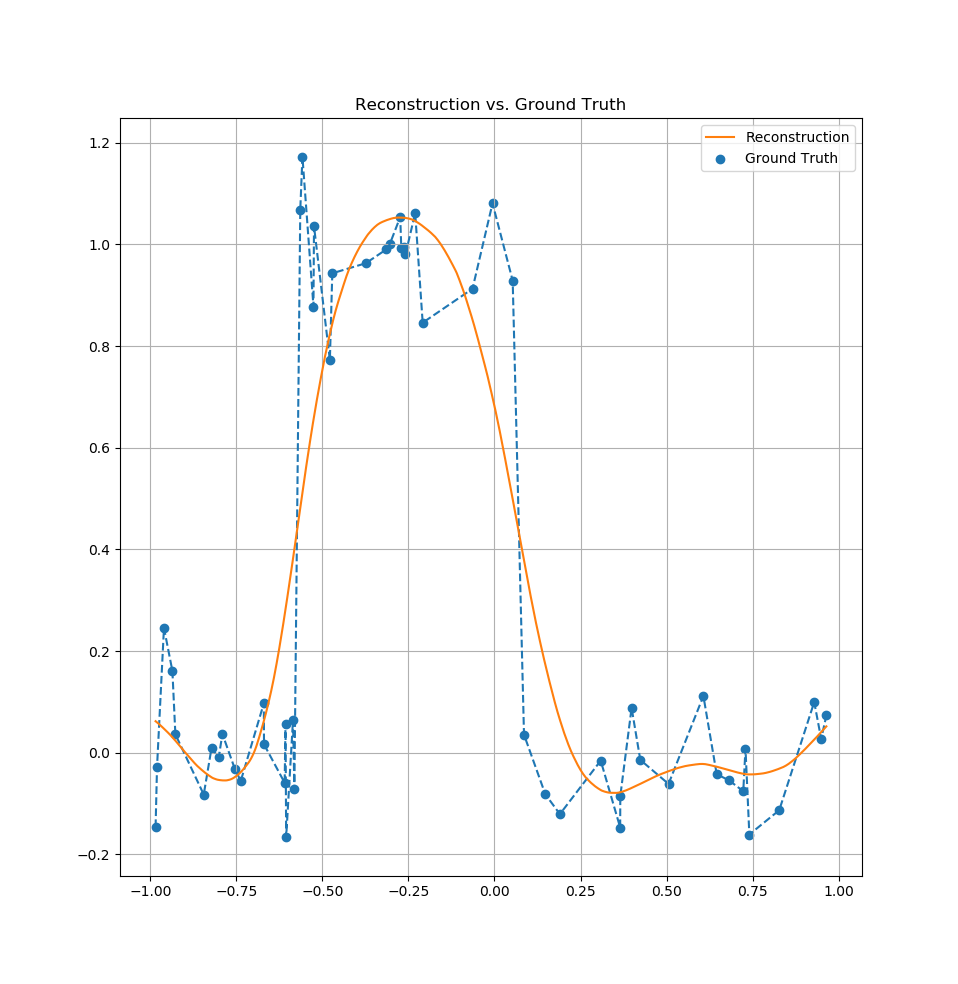
\includegraphics[width=0.45\textwidth]{figures/lazy-square-noise.png}
    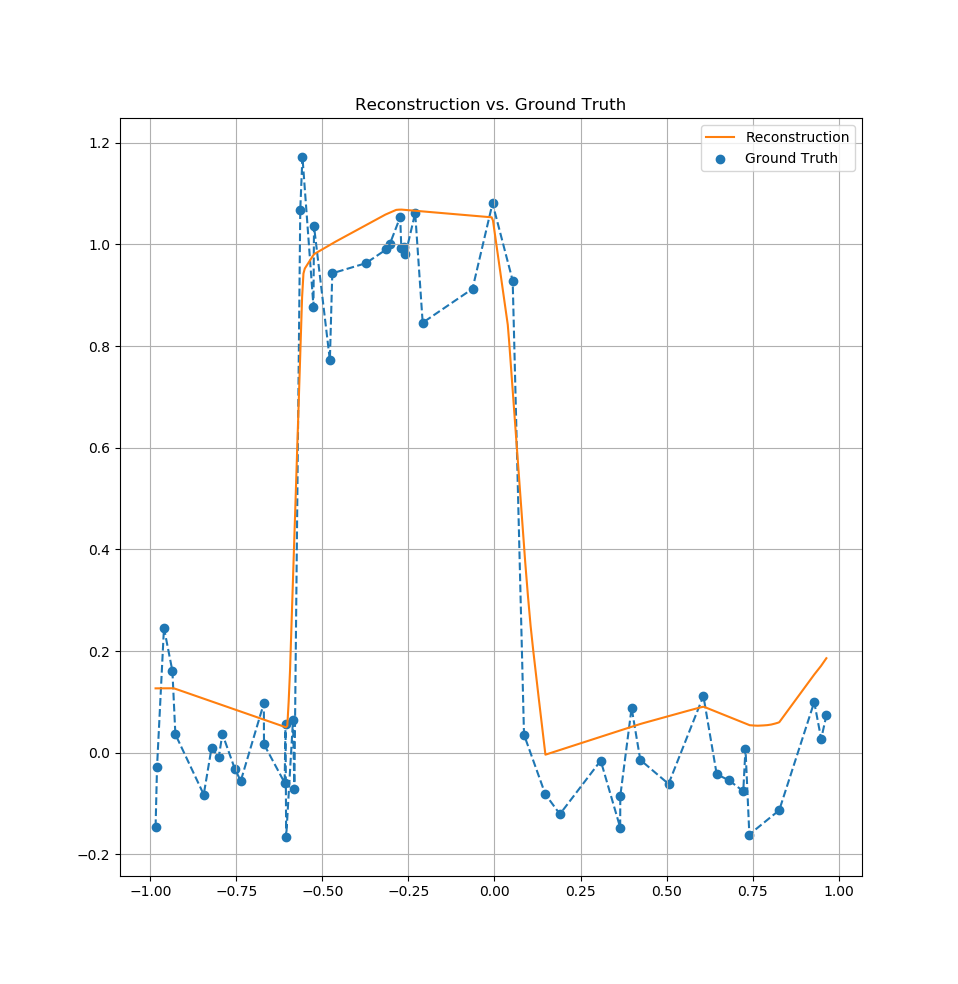
\includegraphics[width=0.45\textwidth]{figures/nonlazy-square-noise.png}
    \caption{The result of fitting a network with 2000 neurons to a square wave with gaussian noise added. Each network was fit with 10k iterations of gradient descent with Nesterov momentum. The left image shows the lazy training regime and the right shows the adaptive kernel regime.}
    \label{fig:early-stopping}
\end{figure}

Note however, that for a fixed kernel, regularization of the least squares problem will yields results similar to gradient descent with early stopping.

A natural consequence of considering only the dynamics of the kernel during training is that once a kernel has been fixed, we can control the smoothness and interpolation of the solution by tuning a single parameter and solving a linear system. We can thus control the quality of the model without retraining the network. 

Figure~\ref{fig:lsq-lazy} shows the result of varying regularization using the tangent kernel and Figure~\ref{fig:lsq-non-lazy} shows the result of regularization using the adaptive kernel.


\begin{figure}
    \centering
    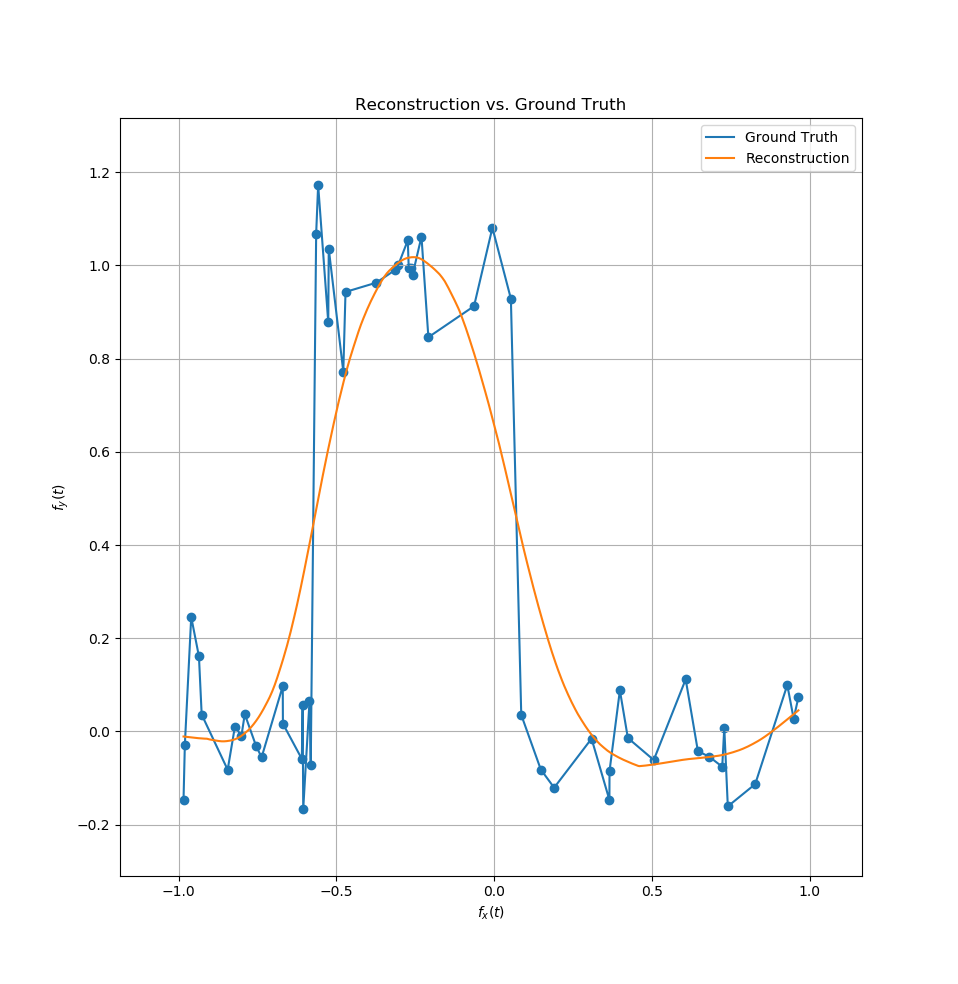
\includegraphics[width=0.32\textwidth]{figures/lazy-square-noise-lsq-1e0.png}
    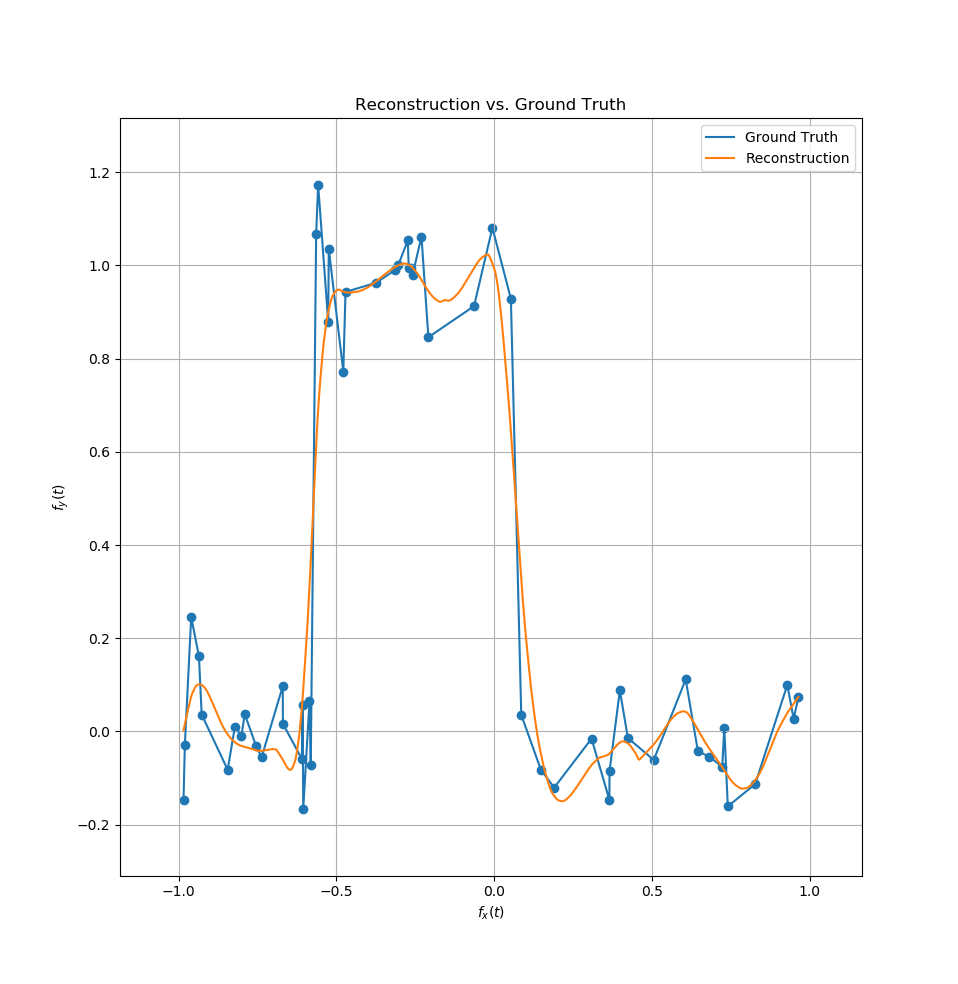
\includegraphics[width=0.32\textwidth]{figures/lazy-square-noise-lsq-1e-1.png}
    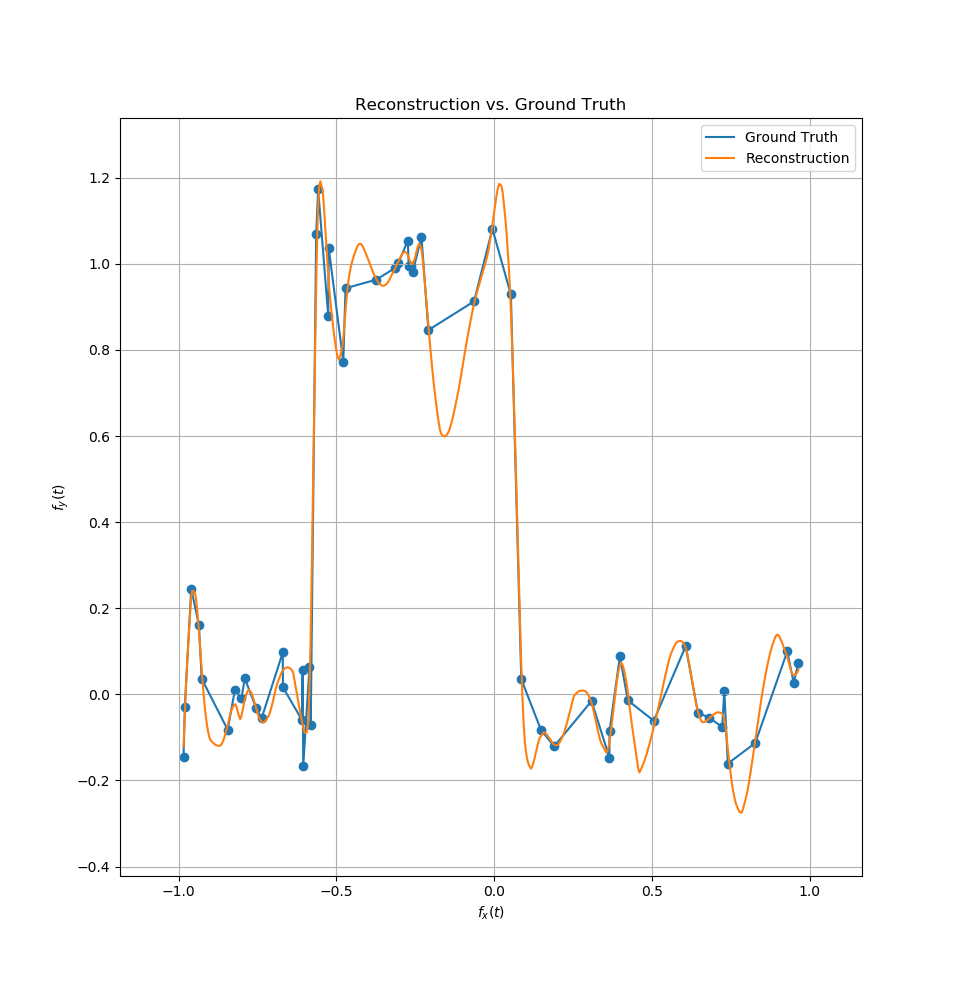
\includegraphics[width=0.32\textwidth]{figures/lazy-square-noise-lsq-1e-2.png}
    \caption{Regularized least squares kernel regression for the lazy kernel. We use different regularization factors (left: 1, mid: 0.1, right: 0.01) to control the smoothness of the solution.}
    \label{fig:lsq-lazy}
\end{figure}


\begin{figure}
    \centering
    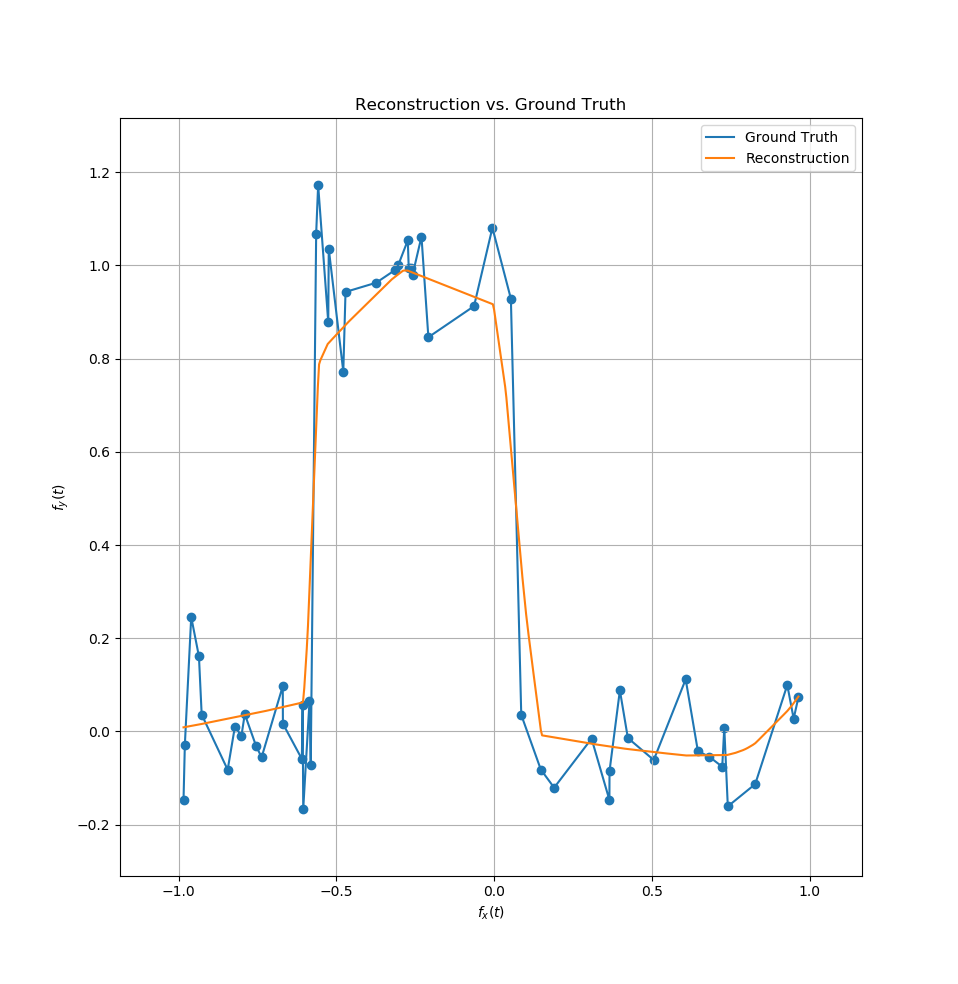
\includegraphics[width=0.32\textwidth]{figures/nonlazy-square-noise-lsq-1e0.png}
    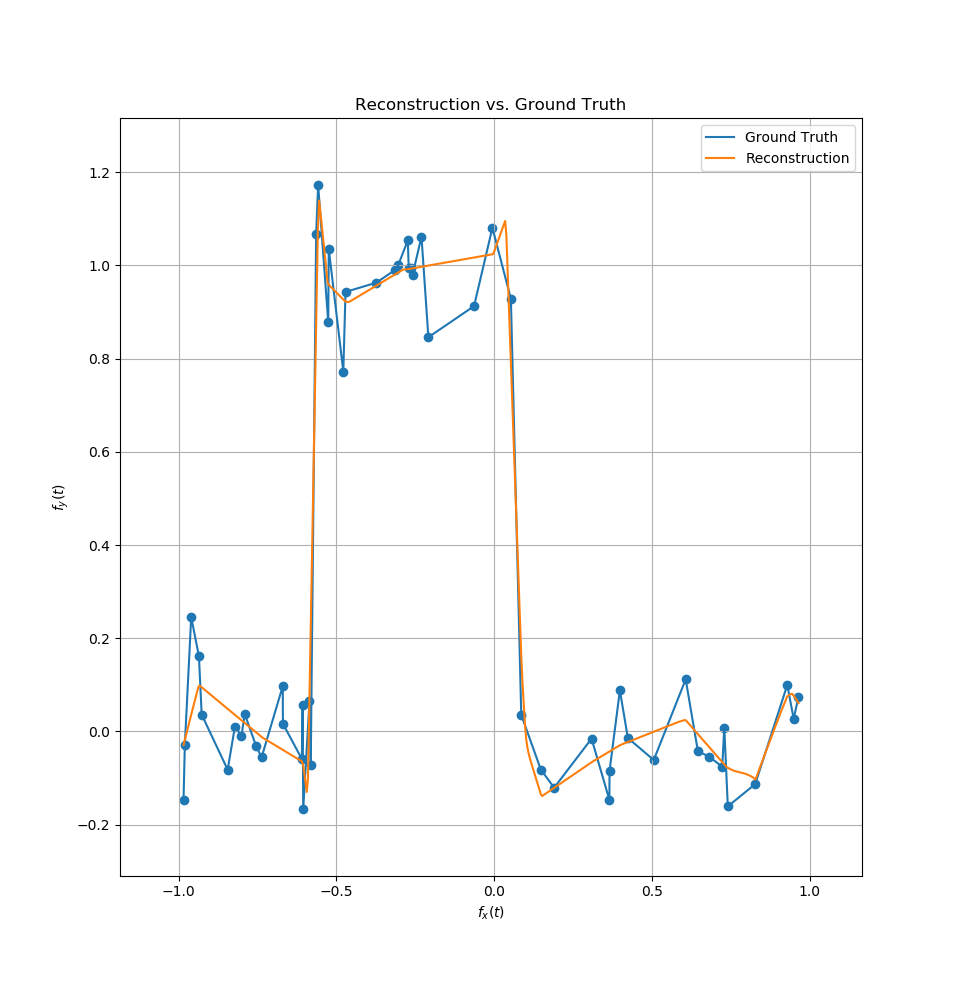
\includegraphics[width=0.32\textwidth]{figures/nonlazy-square-noise-lsq-1e-1.png}
    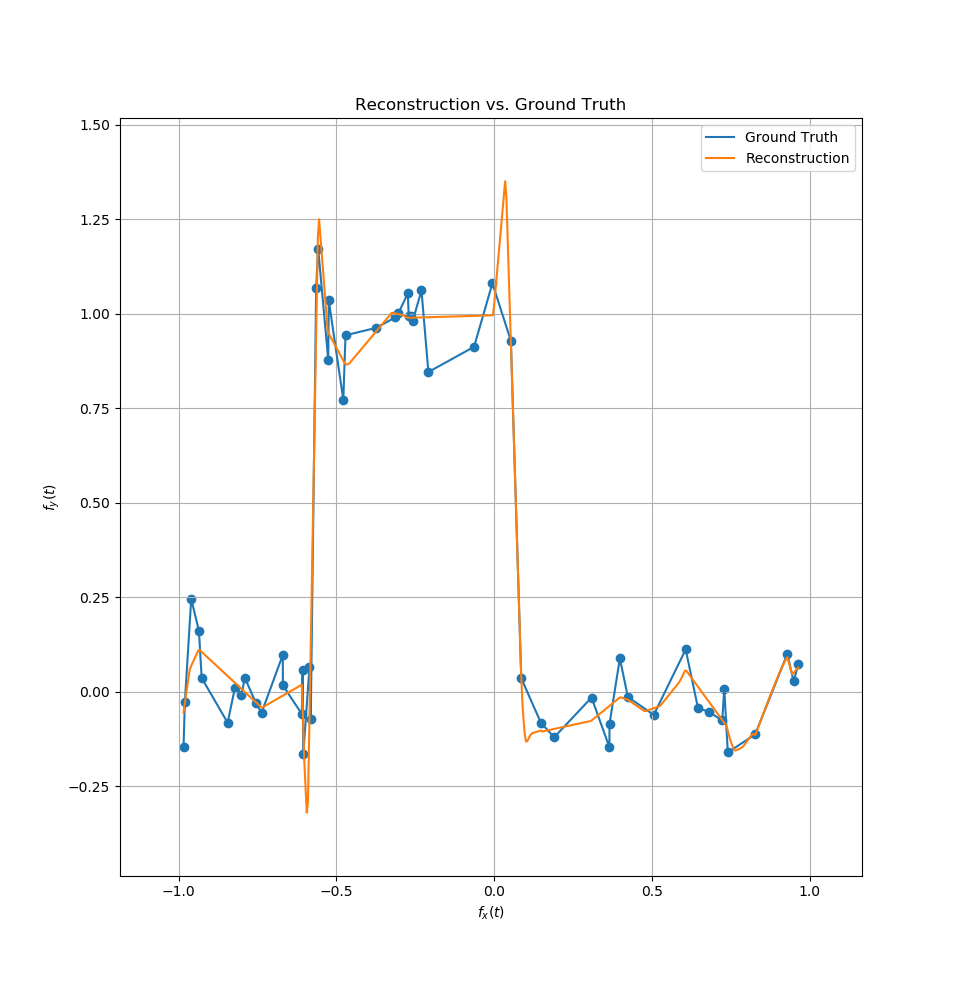
\includegraphics[width=0.32\textwidth]{figures/nonlazy-square-noise-lsq-1e-2.png}
    \caption{Regularized least squares kernel regression for the non-lazy kernel. We use different regularization factors (left: 1, mid: 0.1, right: 0.01) to controll the smoothness of the solution.}
    \label{fig:lsq-non-lazy}
\end{figure}
\input{06_conclusion}
\newpage
\newpage

\section{Practical Implications and Experiments}
\subsection{Outline}
\note{
\begin{itemize}
    \item Verify trajectories match: 2 examples
    \item Delta mostly constant for GD (Appendix)
    \item Cubic spline
    \item 3D plots showing PL vs CS
    \item Same initialization in function space with different initialization has very different dynamics
\end{itemize}
}

In this section we present experimental results illustrating lazy and non-lazy training as well as the robustness to noise arising from flat minima.

\subsection{Preventing Noise Overfitting}
In the over-parameterized regime, a full rank kernel matrix produces interpolatory solutions. In the presence of noisy data, these solutions may be undesirable. Since knots in high curvature regions move faster initially (\todo{better way of saying this}), we can fit features in the data by limiting the number of iterations. Figure~\ref{fig:early-stopping} demonstrates the result for both the tangent and adaptive kernels. 

% {figures/nonlazy-square-noise.png}
\begin{figure}
    \centering
    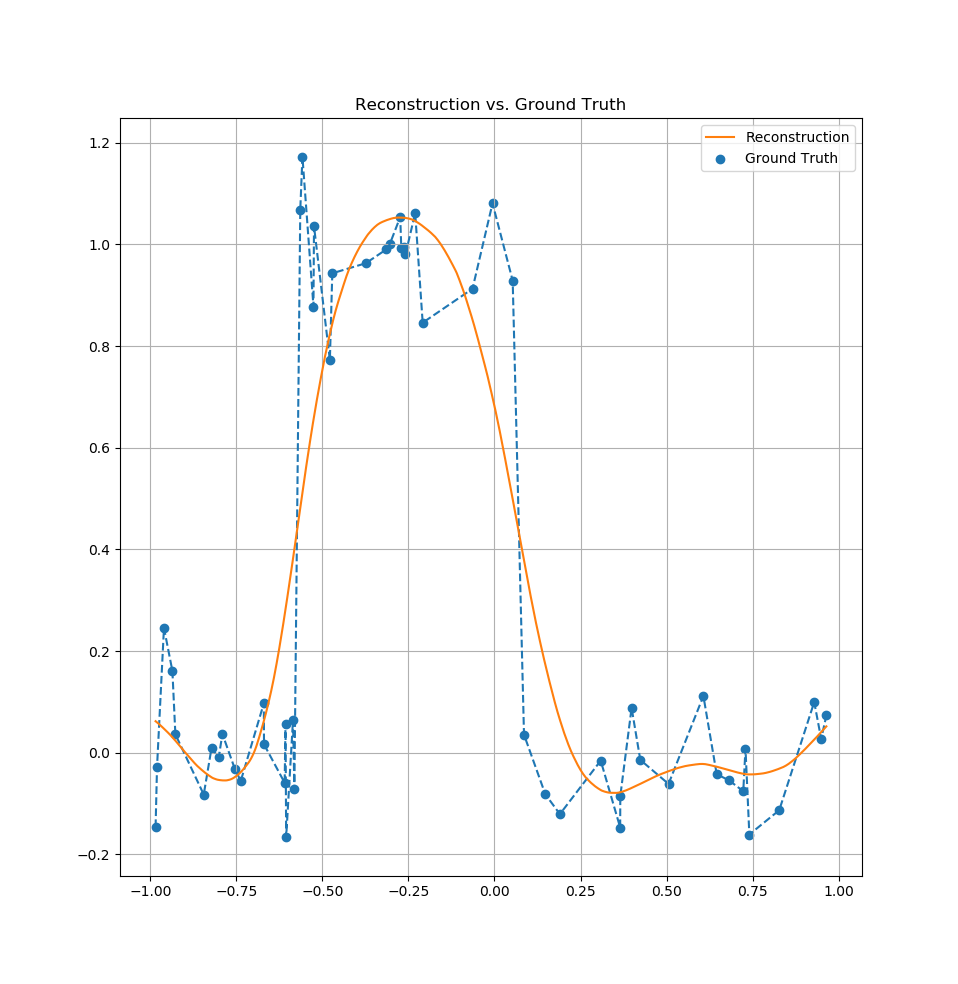
\includegraphics[width=0.45\textwidth]{figures/lazy-square-noise.png}
    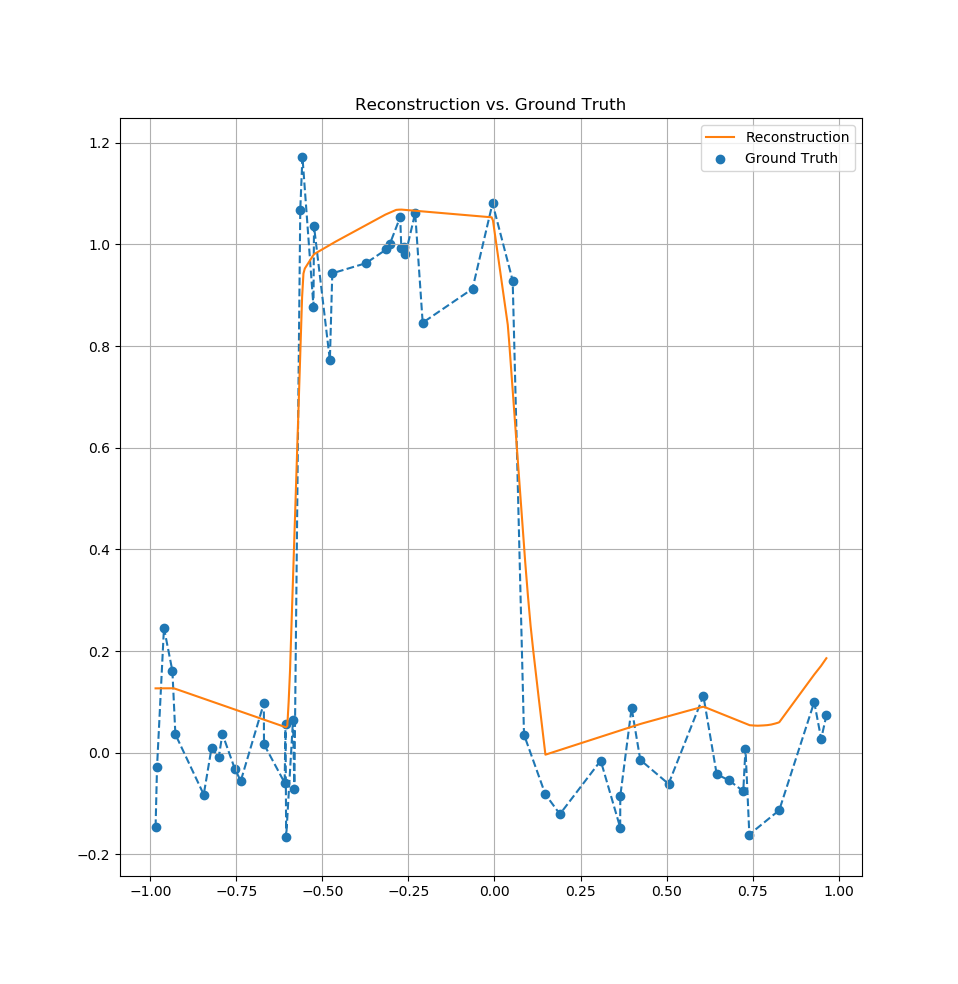
\includegraphics[width=0.45\textwidth]{figures/nonlazy-square-noise.png}
    \caption{The result of fitting a network with 2000 neurons to a square wave with gaussian noise added. Each network was fit with 10k iterations of gradient descent with Nesterov momentum. The left image shows the lazy training regime and the right shows the adaptive kernel regime.}
    \label{fig:early-stopping}
\end{figure}

Note however, that for a fixed kernel, regularization of the least squares problem will yields results similar to gradient descent with early stopping.

A natural consequence of considering only the dynamics of the kernel during training is that once a kernel has been fixed, we can control the smoothness and interpolation of the solution by tuning a single parameter and solving a linear system. We can thus control the quality of the model without retraining the network. 

Figure~\ref{fig:lsq-lazy} shows the result of varying regularization using the tangent kernel and Figure~\ref{fig:lsq-non-lazy} shows the result of regularization using the adaptive kernel.


\begin{figure}
    \centering
    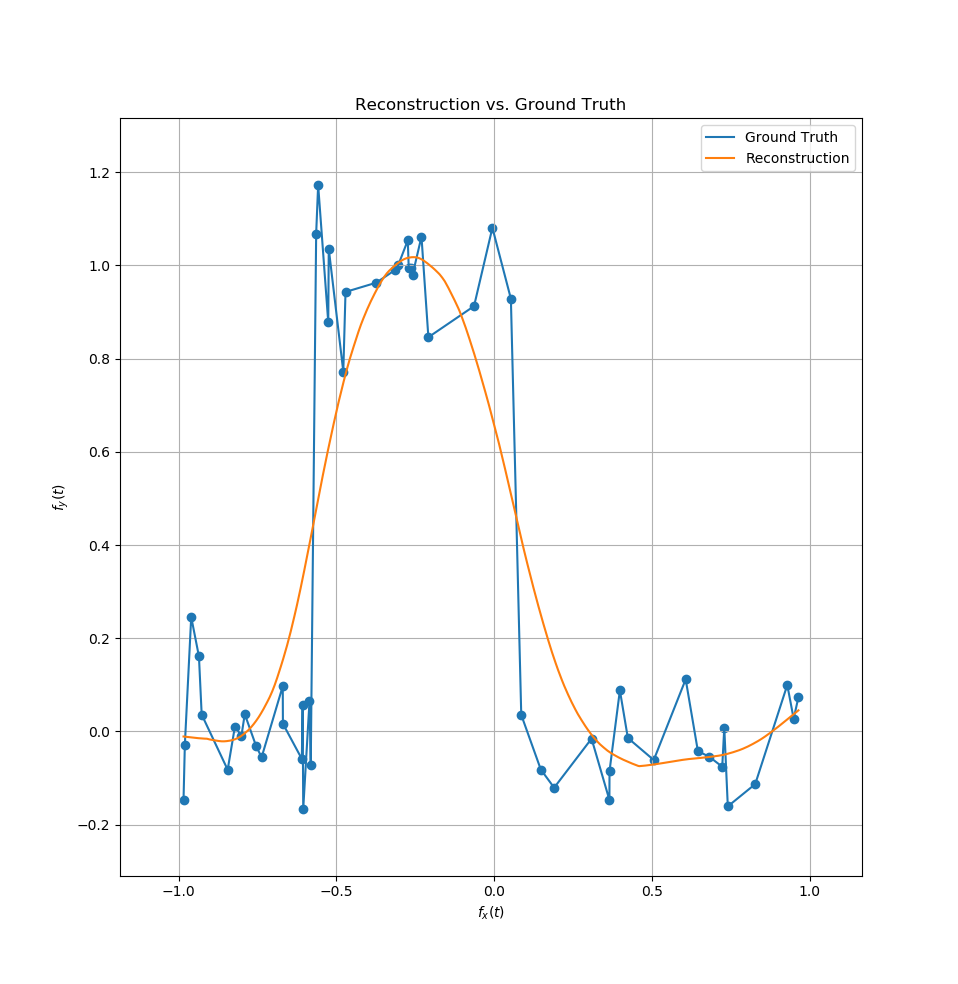
\includegraphics[width=0.32\textwidth]{figures/lazy-square-noise-lsq-1e0.png}
    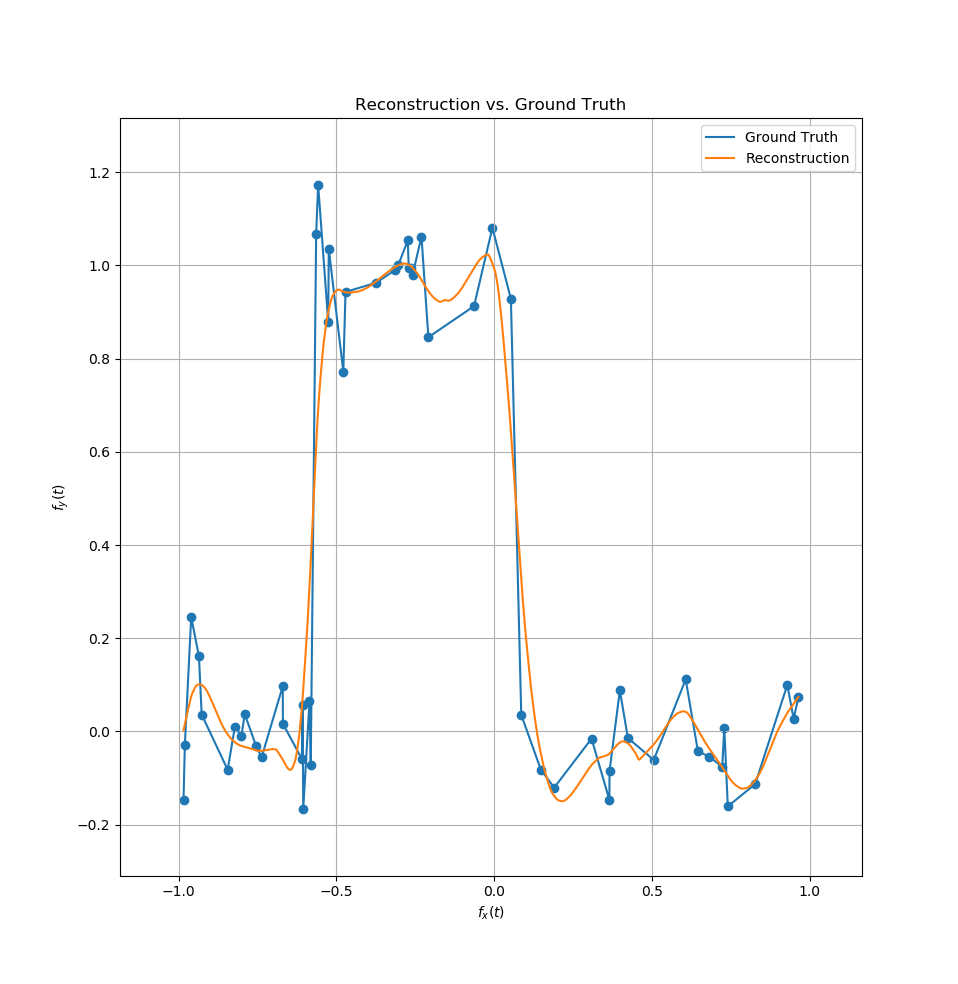
\includegraphics[width=0.32\textwidth]{figures/lazy-square-noise-lsq-1e-1.png}
    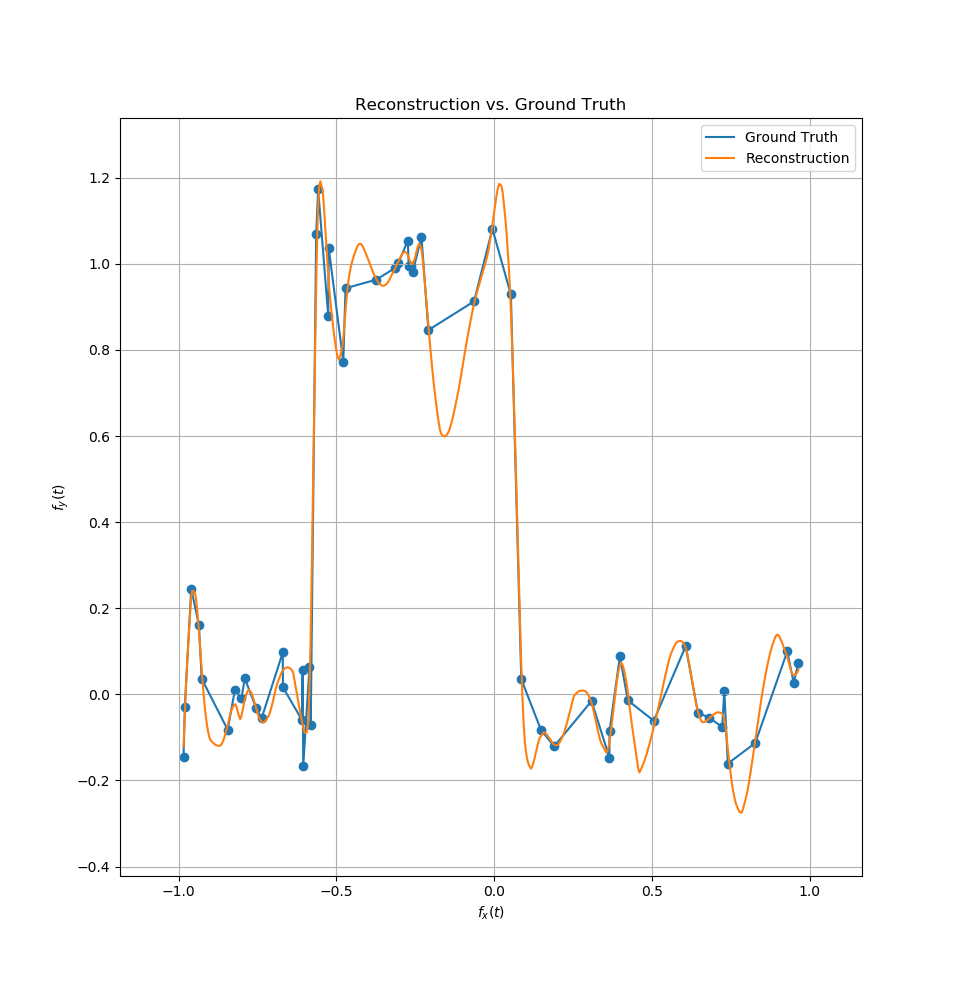
\includegraphics[width=0.32\textwidth]{figures/lazy-square-noise-lsq-1e-2.png}
    \caption{Regularized least squares kernel regression for the lazy kernel. We use different regularization factors (left: 1, mid: 0.1, right: 0.01) to control the smoothness of the solution.}
    \label{fig:lsq-lazy}
\end{figure}


\begin{figure}
    \centering
    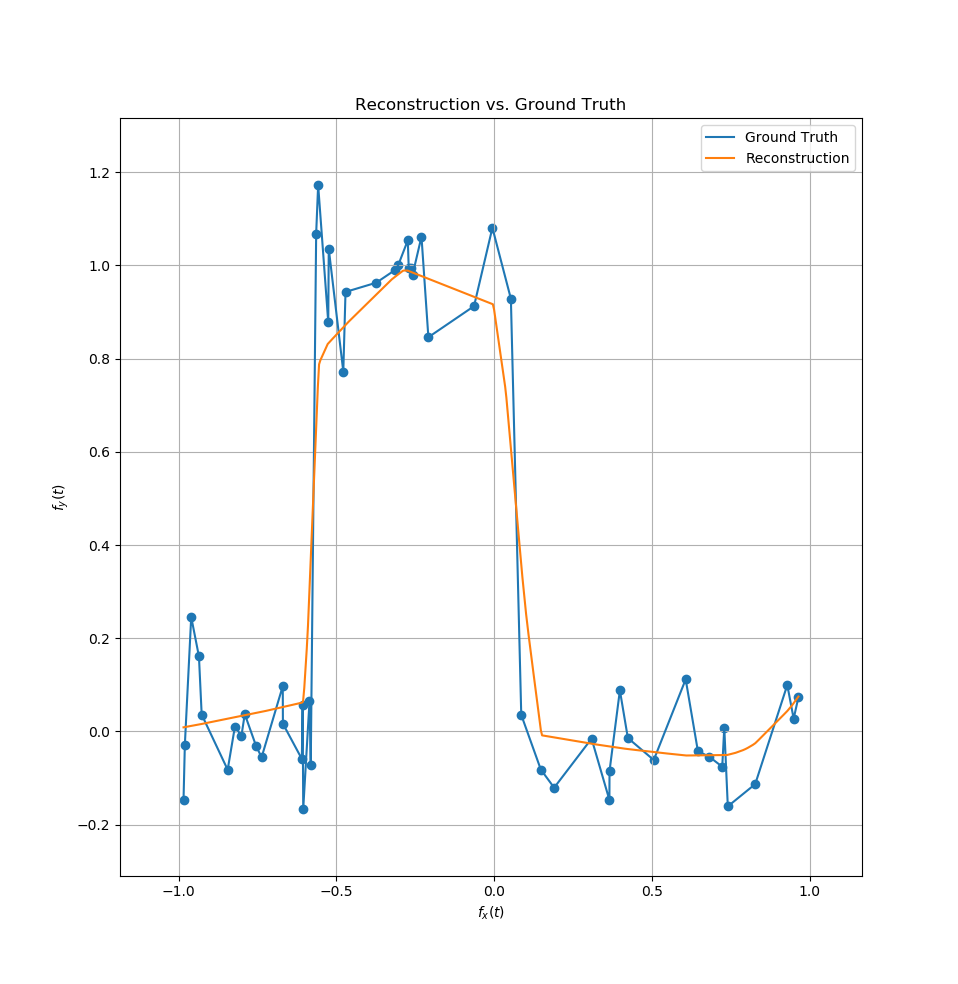
\includegraphics[width=0.32\textwidth]{figures/nonlazy-square-noise-lsq-1e0.png}
    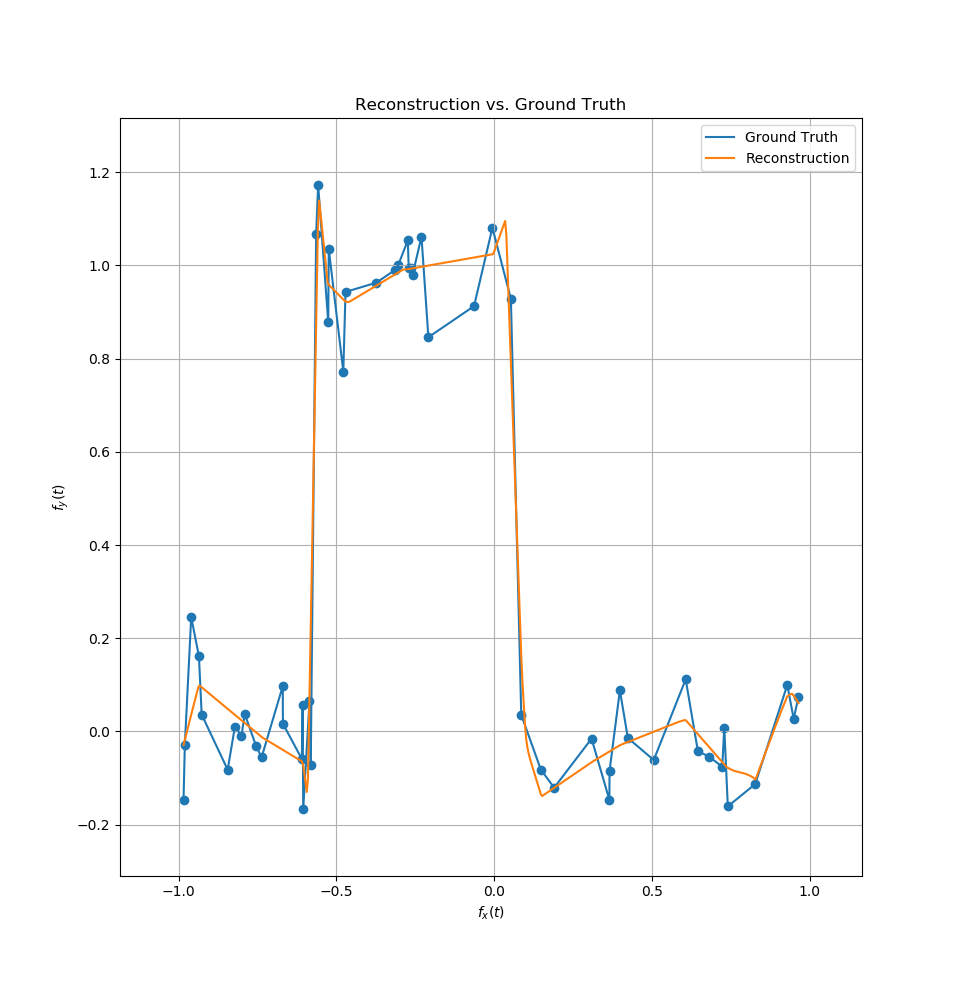
\includegraphics[width=0.32\textwidth]{figures/nonlazy-square-noise-lsq-1e-1.png}
    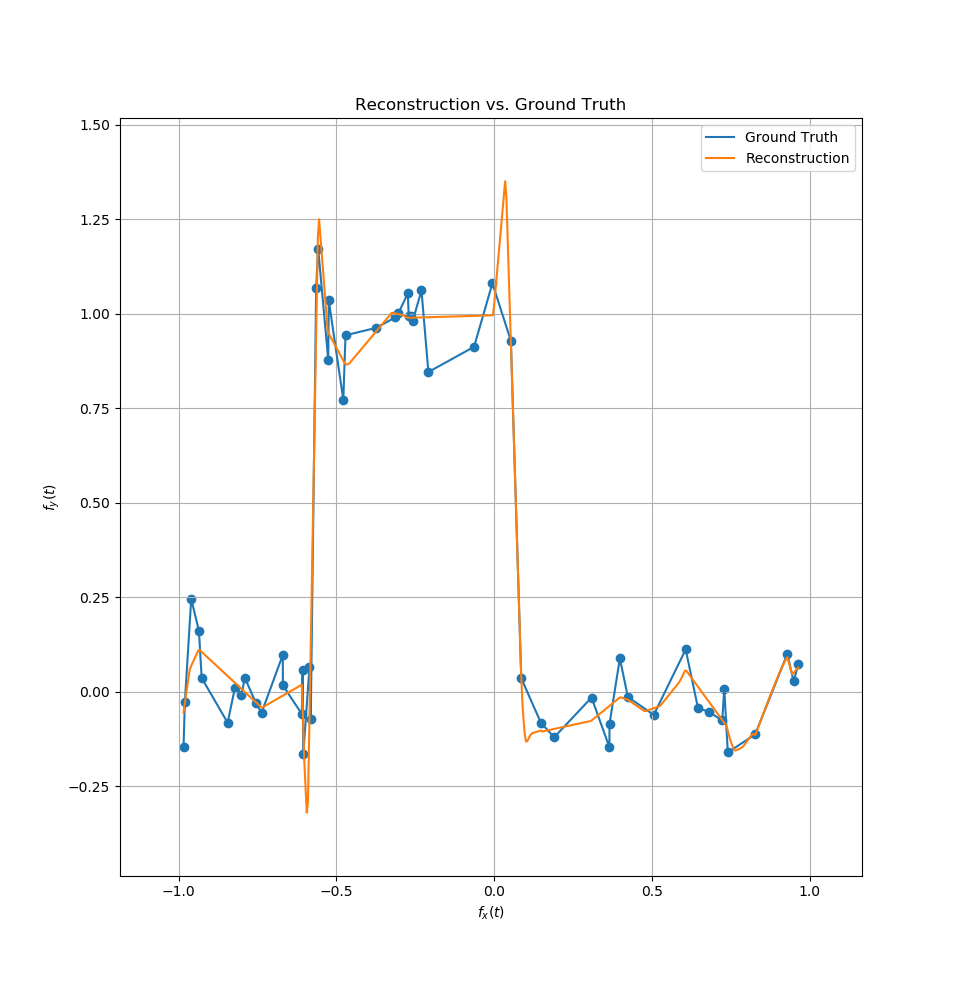
\includegraphics[width=0.32\textwidth]{figures/nonlazy-square-noise-lsq-1e-2.png}
    \caption{Regularized least squares kernel regression for the non-lazy kernel. We use different regularization factors (left: 1, mid: 0.1, right: 0.01) to controll the smoothness of the solution.}
    \label{fig:lsq-non-lazy}
\end{figure}

\section{Global Training Dynamics}
% The invariants $\delta_i$ allow us to present a concrete framework for understanding the global dynamics of neurons in terms of their initialization. We can understand the global dynamics of neural networks in terms of two regimes corresponding to eigenvectors of $M_\delta$ in the previous section: \emph{Radial training} and \emph{Tangential training}. 

In this section, we consider the extreme cases of initialization: $\delta \ll -\|\xi\|$ (radial dynamics) and $\delta \gg \|\xi\|$ (tangential dynamics). This corresponds to training only the bottom and only the top layer of the network, respectively. 

% We show that lazy training occurs when $\delta \ll 0$ (radial motion in the reduced parameters). We demonstrate that in this regime, the network is biased towards ``smooth'' solutions. At the other end of the spectrum \cite{maennel2018gradient} observe that small initializations lead to a quantization effect of the weight vectors independent of the size of the network. This phenomenon occurs more prominently as $\delta$ grows larger. Furthermore, we describe precisely where the the weight vectors concentrate in terms of the input samples. We also note that the samples at which neurons concentrate are not fixed, but are dynamical quantities which depend on the activation pattern and on the residuals.

% We note that scaling the gradient flow is equivalent to scaling the distributions from which the initial parameters, $\theta$ are sampled, thus we can control the value of $\delta$ by either rescaling the gradient flow or changing the initial distribution of $\theta$.


\subsection{Radial Training}

\note{We should say that radial training is what happens with the standard initialization using pytorch}

In pure radial regime, we are only learning the outer layer parameters and leaving the inner parameters fixed. This corresponds to \emph{kernel learning}~\note{Cite someone}. In the overparameterized setting, we wish to solve

\begin{equation}\label{eq:lsq_overparameterized}
\begin{gathered} 
    \text{minimize } ||c||^2\\
    \text{subject to } M_x(a, b) c = y
\end{gathered}
\end{equation}

which is strictly convex with convex constraints. Writing $M = M_x(a,b)$, we have that solution to \eqref{eq:lsq_overparameterized} is given by $c = M^T (M M^T)^{-1} y$. We define the kernel

\begin{equation}
    K_{(a,b)}(x,x') = \sum_{i=1}^m [a_i x + b_i]_+[a_i x' + b_i]_+
\end{equation}


The optimized function is given by

\begin{equation}
    f(x) = \sum_{j=1}^s v_j K(x_j, x)
\end{equation}


where $v = K(x_i,x_j)^{-1} y$. Of course, this closed form solution only corresponds to the point of convergence of the gradient flow only if $c(0) = 0$. The more general dynamics of the flow can be similarly derived in terms of the kernel $K$ (see Appendix). Furthermore, it is known in this setting that early stopping for
gradient descent will act as a regularizes as these eigenfunctions of $K$ typically correspond to lower frequency features of the function being fit \note{cite}.







\paragraph{Infinite width limit}
% We analyze the behavior of the \emph{limit kernel} as the number of weights $m \rightarrow \infty$ in the radial regime. We show that the overparameterized least squares problem in this setting minimizes curvature. Furthermore, for 1D functions, the network functions are natural cubic spines. 
In the infinite width ($m = \infty)$ limit, the parameters, $\theta$ become densities $\theta(s) = (a(s), b(s), c(s))$. Assuming that $s \in [k_1, k_2], x \in [k_1, k_2]$, then we can write the function $f$ as

\begin{equation}
    f(x) = \int_{k_1}^{k_2} c(s) [a(s) x + b(s)]_+ ds
\end{equation}

and the least squares problem becomes
\begin{equation}
    \begin{gathered}
    \text{minimize } ||c(s)||^2\\
    \text{subject to } \int_{k_1}^{k_2} c(s) [a(s)x_i + b(s)]_+ ds = y_i
    \end{gathered}
\end{equation}

\begin{lemma}\label{le:curvature}
The second derivative of $f(x)$ is the parameter density $c(s)$. i.e. 
\begin{equation*}\partial_x^2 f(x) = c(s)\end{equation*}
\end{lemma}
\begin{proof}
\todo{TODO}
\end{proof}

Thus, the quantity $||c(s)||^2 = ||\partial_x^2 f(x)||^2$ being minimized is the \emph{curvature}. Thus, we can view the radial regime as an implicit bias towards ``smooth'' functions.



For 1D functions with knots initialized from a uniform distribution, we give an exact equation for the limit kernel. 

\begin{lemma}\label{le:cubic_spline}
Assume that the knots $e(s) =\ -\frac{b(s)}{a(s)} ~ U(k_1, k_2)$, then the inifinite width kernel, $K(x, y)$ is a cubic polynomial in $x$ and $y$
\end{lemma}
\begin{proof}

We can rewrite the kernel,
\begin{equation}
    K(x, y) = \int_{k_1}^{k_2} [a(s)x + b(s)]_+ [a(s)y + b(s)]_+ ds
\end{equation}

in terms of the knots $e(s)$

\begin{equation}
    K(x, y) = \int_{k_1}^{k_2} \tau(x, s) \tau(y, s) a(s)^2 (x - e(s)) (y - e(s)) ds
\end{equation}

where $\tau(x, s) = \mathds{1}[a(s)x + b(s) \geq 0]$. $a(s)$. Sicne the knots $e(s) = -\frac{b(s)}{a(s)}$ are uniformly distributed, we can write $e(s) = s$ which implies $-b(s) = s a(s)$. In this case, we can assume without loss of generality that $v(s) = -s$ and $u(s) = 1$. We then rewrite the kernel

\begin{equation}
    \begin{aligned}
    K(x, y) &= \int_{k_1}^{k_2} \tau(x, s) \tau(y, s) (x - s) (y - s) ds\\
            &= \int_{k_1}^{\min(x, y)} (x - s) (y - s) ds\\ 
            &= s xy - \frac{1}{2} s^2 (x + y) - \frac{1}{3} s^3 \bigg\rvert_{k_1}^{\min(x, y)}
    \end{aligned}
\end{equation}

which is a cubic function in $x$ and $y$.
\end{proof}

Recall that for full rank $M_x(a,b)$, the function $f(x)$ interpolates the samples, $x_i$. Thus, a corollary to Lemmas \ref{le:curvature} and \ref{le:cubic_spline} is that for uniform knot initialization, 1D neural network functions are cubic splines interpolating the samples. Figure~\ref{fig:cubic_splines} shows the convergence to a cubic spline as the number of neurons grows large. \note{We need to cite the paper on linear splines here.} 

\begin{figure}\label{fig:cubic_splines}
    \centering
    \minipage{0.33\textwidth}
    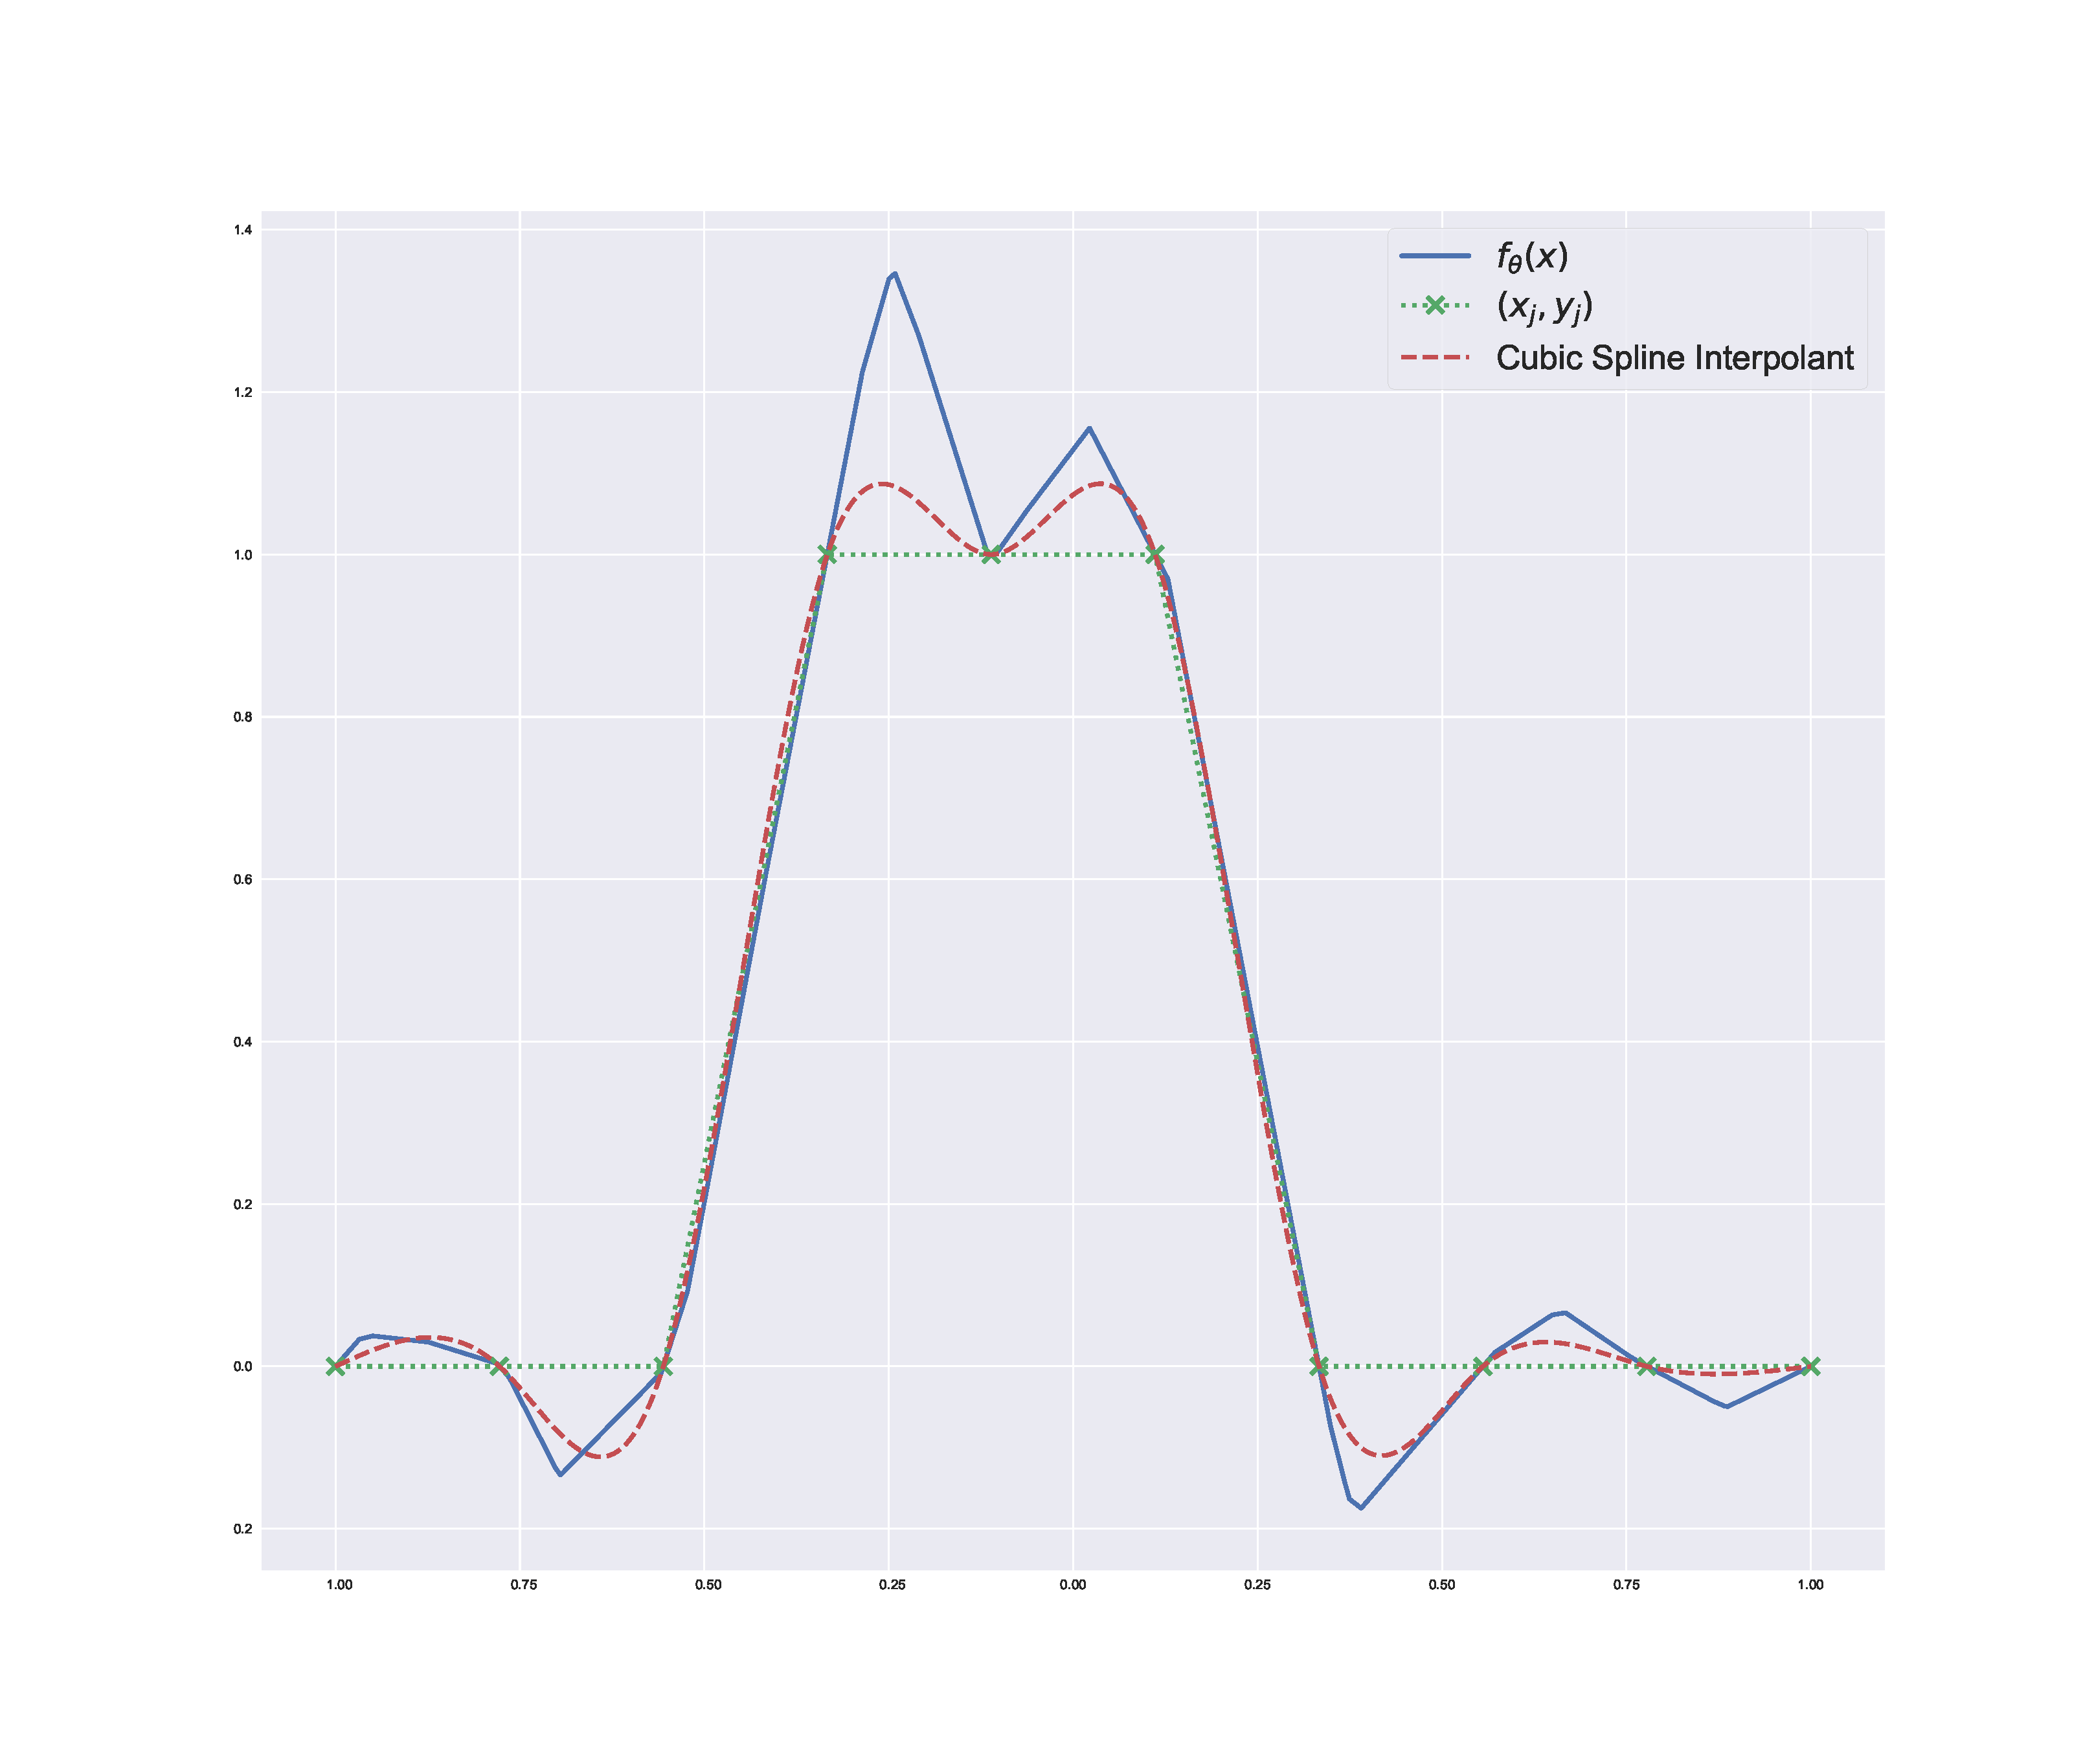
\includegraphics[width=\linewidth]{figures/cubic_spline100.pdf}
    \endminipage\hfill
    \minipage{0.33\textwidth}
    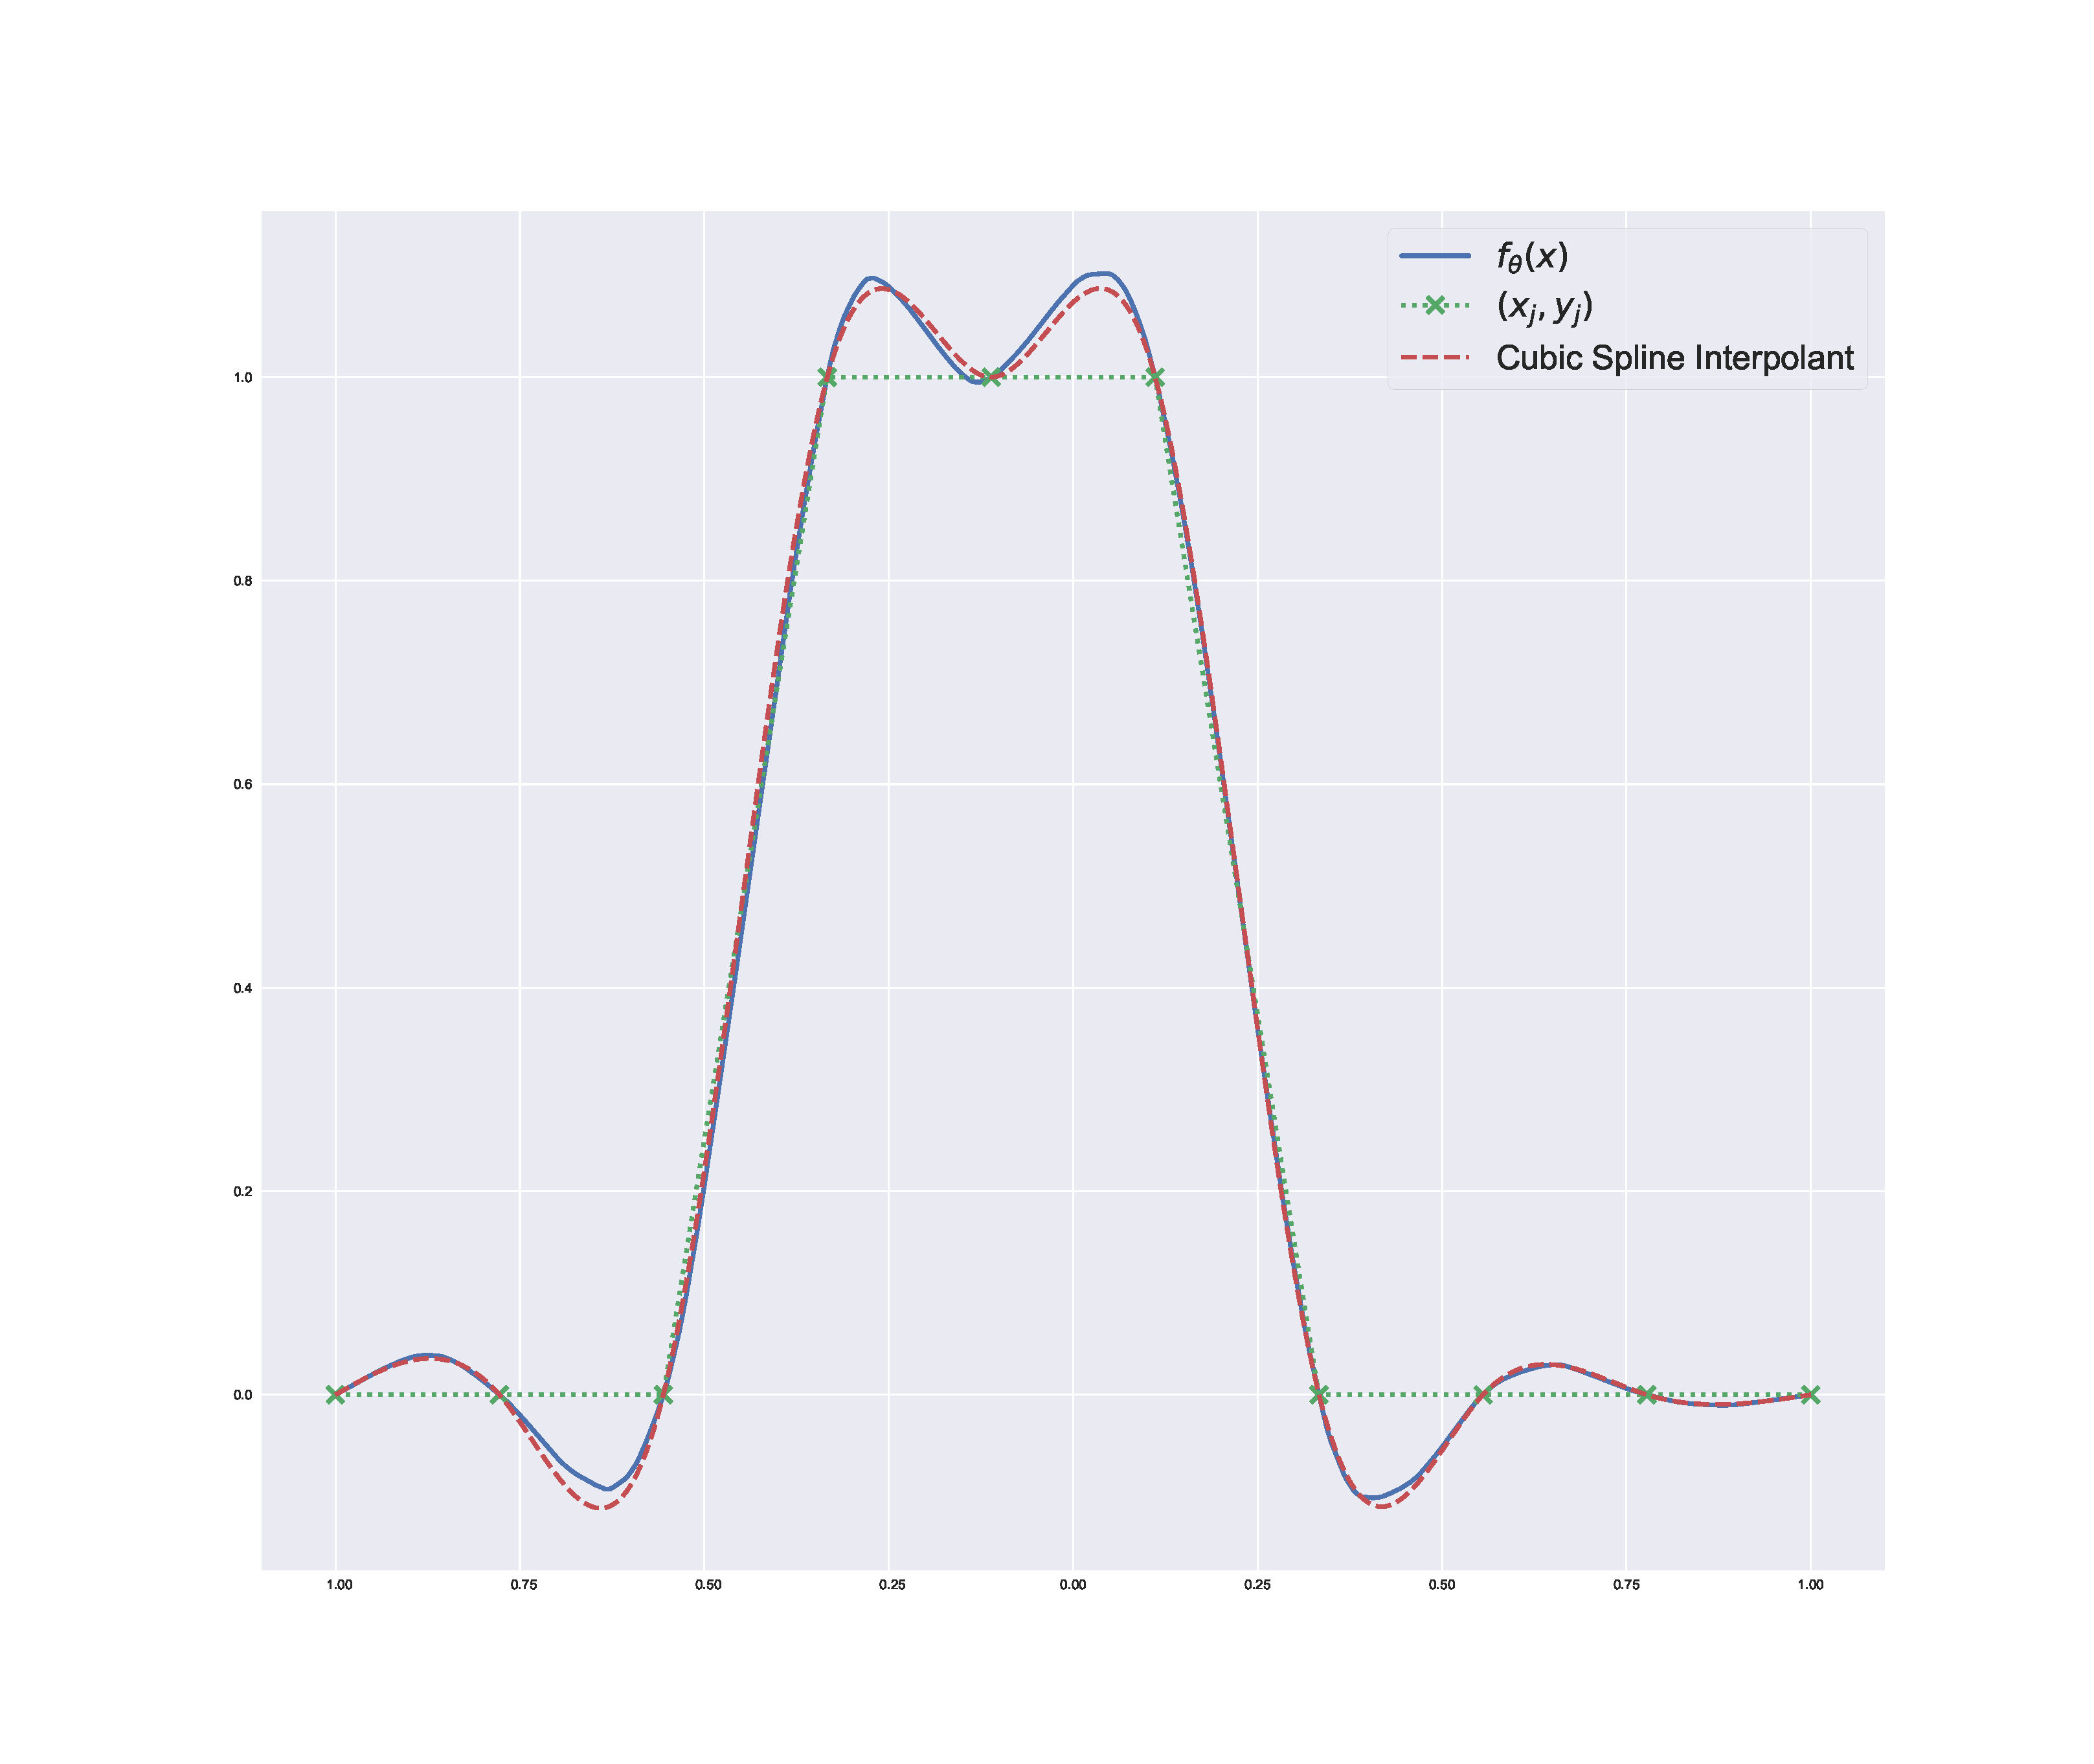
\includegraphics[width=\linewidth]{figures/cubic_spline_1k.pdf}
    \endminipage\hfill
    \minipage{0.33\textwidth}
    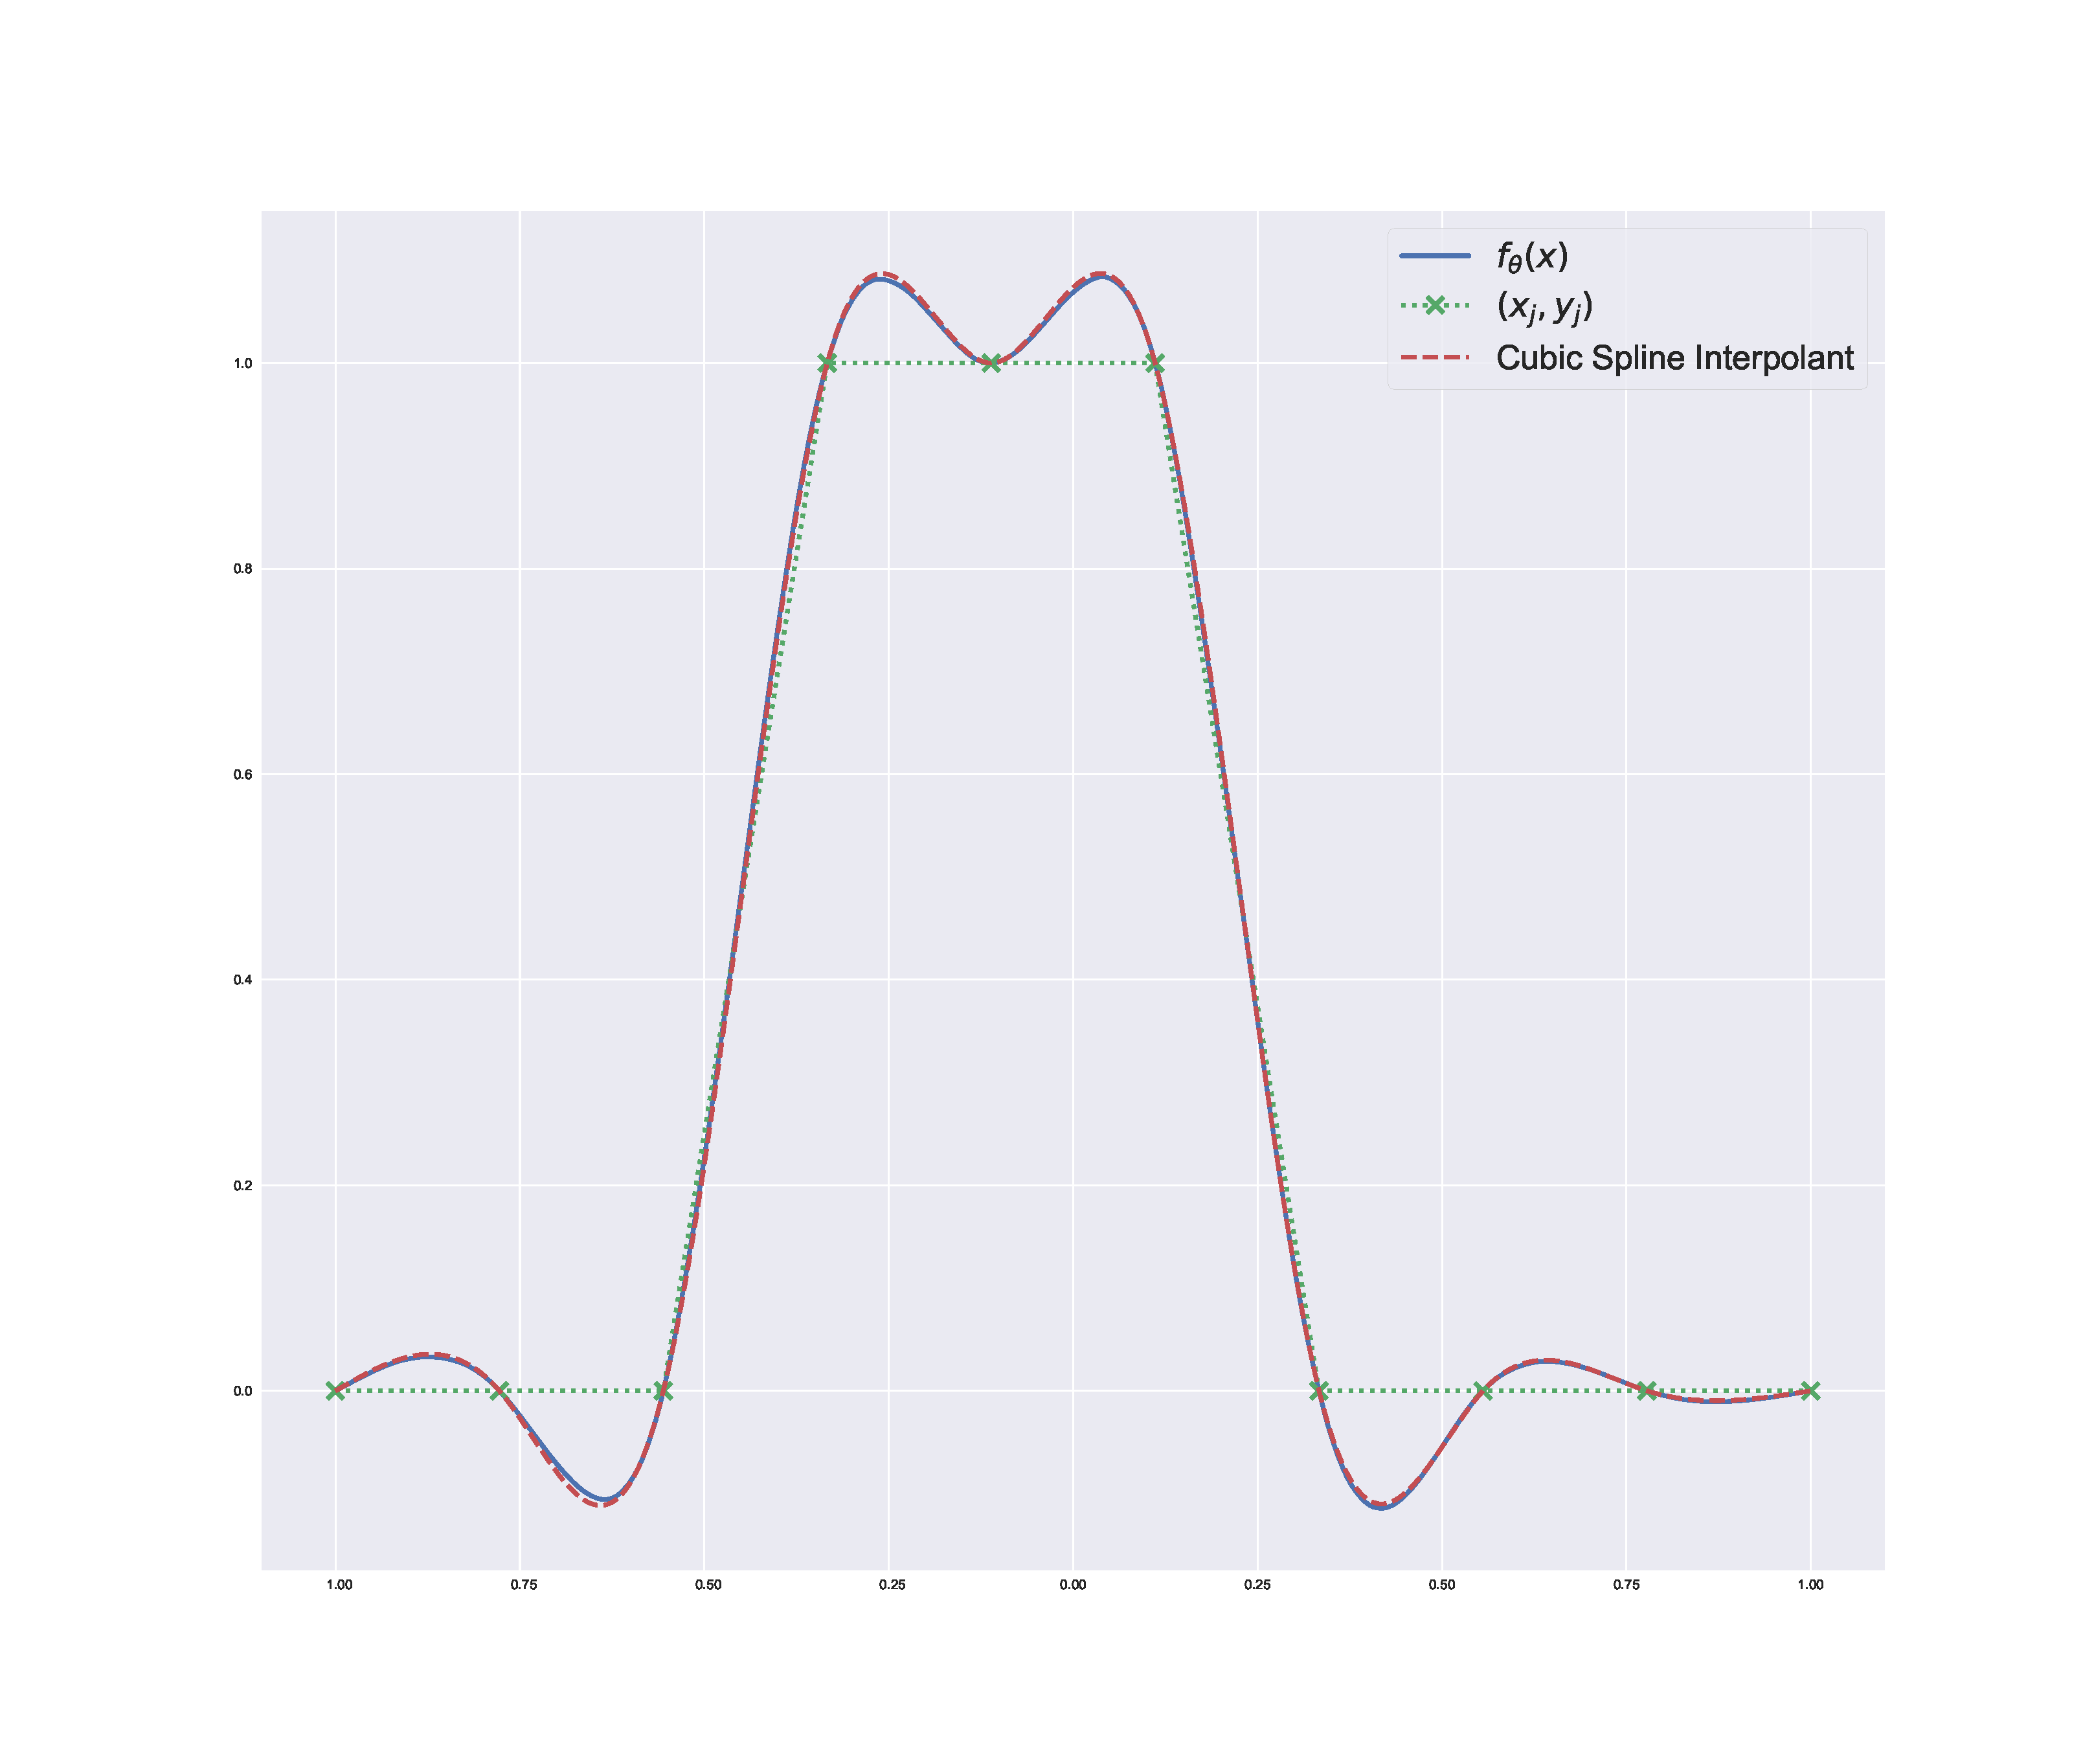
\includegraphics[width=\linewidth]{figures/cubic_spline_10k.pdf}
    \endminipage
    \caption{Regression in the purely tangential regime ($\delta = -\infty$) using varying knots. We observe that as the number of knots increases, the function, $f_\theta$ converges to a cubic spline interpolant with $\partial_x^2 = 0$ on the boundary.}
    \label{fig:radial_trajectores}
\end{figure}



















\subsection{Tangential Training, $\delta \gg \|\xi\|$}


\note{Use interesting?}

Recall that Lemma~\ref{le:pw_continuous} states that the gradient field $\nabla \tilde{L}$ is piecewise continuous. An important consequence of this result is that the gradient field could point in opposite directions on the boundary of a sample (\todo{Figure \ref{fig:todo}}). In this case, a neuron could get stuck along the boundary for that sample and only be able to move radially. We call the samples at which neurons get stuck \emph{attractive}. The existence of attractive samples leads to neurons piling up at samples, biasing the functions $f(x)$ to be piecewise linear with a small number of pieces.

We now give a precise condition for when a sample is attractive. We also show that the set of attractive samples is a dynamical quantity which depends only on the activation.

Recall that in the reduced parameter space, a sample $x_i$ corresponds to a line in the $(u, v)$ plane. The sample $x_i$ is \emph{attractive} if the loss gradient in the reduced parameters $\nabla \tilde{L}$ points in opposite directions on either side of this line. 

Formally, we can express attractiveness as a condition on the time derivative of the knots $e_i(t)$. 

\begin{equation}\label{eq:moving_knots}
\partial_t e_i(t) = \frac{-a_i \partial b_i + b_i \partial a_i}{a_i^2} = c_i\frac{- a_i \sum_
{j=1}^s
\tau_{ij} r_j + b_i \sum_
{j=1}^s \tau_{ij} x_j r_j}{a_i^2} = \frac{\sum_{j=1}^s \tau_{ij}c_i(-a_i
+x_j b_i)r_j}{a_i^2}
\end{equation}

\note{Possibly useful to frame attractiveness/interestingness:}
\begin{definition}
Consider a function of the form $h(\bm w) = \sum_{i=1}^s r_i [\langle \bm w,\bm x_i\rangle ]_+$ with $\bm w, \bm x_i \in \RR^2$ and $r_i \in \RR$. We say that $\hat{ \bm w} \in \mathbb S^1$ is a \emph{stable direction} if $\hat{ \bm w} \in \alpha \partial h(\hat {\bm w})$ for some $\alpha > 0$ (perhaps give more intuitive definition/picture?).
\end{definition}

A stable direction can either be on the boundary or on the internal part of a segment. From~\eqref{eq:moving_knots}, we are interested in the stable directions for $h((a_i,b_i)) = \epsilon_i \sum_{i=1}^s r_j [(-a_i + x_jb_j)]_+$. Stable directions on the boundaries are ``interesting points''.


\note{Think about how to present this}

Assume that the samples $x_1 < x_2 < \ldots < x_s$ are ordered and suppose that the knot $e_i$ lies on the sample $x_k$, i.e. $e_i(t) = x_k$. Denoting $r = (r_j(\theta))_{j=1}^s$ as the vector of residuals, we have that a the sample $x_k$ is attractive if

\begin{equation}
\begin{aligned}
    &\sum_{j=1}^{k-1} (1+x_j x_k) r_j \lessgtr 0 \quad \mbox{ and } \qquad \sum_{j=1}^k (1+x_j x_k) r_j \gtrless 0, \quad \mbox{ or }\\
    &\sum_{j=k}^s (1+x_j x_k) r_j \gtrless 0 \quad \mbox{ and } \qquad \sum_{j=k+1}^{s} (1+x_j x_k) r_j \lessgtr 0.\\
\end{aligned}
\end{equation}

If $z_j = (1,x_j) r_j$, we can rewrite this as

\begin{equation}
\begin{aligned}\label{eq:attractor_cond}
    &\sum_{j=1}^{k-1} \langle z_k , z_j \rangle < 0 \quad \mbox{ and } \qquad \sum_{j=1}^{k} \langle z_k, z_j \rangle > 0, \quad \mbox{ or }\\
    &\sum_{j=k}^{s} \langle z_k , z_j \rangle > 0 \quad \mbox{ and } \qquad \sum_{j=k+1}^{s} \langle z_k, z_j \rangle < 0.\\
\end{aligned}
\end{equation}


This can be written in terms of the Gram matrix $Z_{ij} = (\langle z_i, z_j\rangle)$.

\paragraph{Dynamics of Attractive Samples}

The attractiveness condition \eqref{eq:attractor_cond} is a dynamic quantity depending on the residuals $r(\theta)$ as well as the samples, $x$. A sample can only change from attractive to unattractive or vice-versa when the activation matrix $\tau$ changes.

\begin{lemma}
If the truth value of the condition \eqref{eq:attractor_cond} changes at time $t$, then the activation matrix, $\tau$ must also change at time $t$.
\end{lemma}
\begin{proof}
\todo{TODO}
\end{proof}

Qualitatively, a sample is attractive when there is a large change in sign between the average residual on one side of the sample and the sample itself. Attractive samples on the ''peaks`` and ``valleys of the of the residual. As with the residual case, low frequency features in the data tend to be fit first with high frequency features being fit later. \todo{Figure~\ref{fig:todo}} shows an example of this behavior.



























\iffalse
\subsection{Old}
% It is easy to verify that the eigenvalue-eigenvector pairs of $K(\xi)$ are
% $(\beta a^2+ \beta b^2 + \alpha c^2, (a,b))$ and $(\alpha c^2, (-b,a))$, which correspond to radial and tangential components of $(u, v)$. From this we deduce that


% \begin{itemize}
%     \item If $\alpha c^2 \ll \beta (a^2 + b^2)$, which means that $\delta <
%     0$, then $\xi_i'(t) \propto (a(t),b(t))$, and the reduced neuron
%     moves~\emph{radially}.
%     \item If $\alpha c^2 \gg \beta (a^2 + b^2)$, which means that $\delta > 0$, then
%     $\xi_i'(t) \propto \nabla^\xi(\xi)_i$, so the reduced neuron follows themaybePres
% \end{itemize}



\paragraph{Node dynamics.}

\begin{equation}
\dot e_i(t) = \frac{-\dot b_i a_i + \dot a_i b_i}{a_i^2} = c_i\frac{- a_i \sum_
{j=1}^s
\tau_{ij} r_j + b_i \sum_
{j=1}^s \tau_{ij} x_j r_j}{a_i^2} = \frac{\sum_{j=1}^s \tau_{ij}c_i(-a_i
+x_j b_i)r_j}{a_i^2}
\end{equation}

If $e_i(t) = x_k$, that is, $-b_i = x_k a_i$, then

\begin{equation}
\dot e_i(t) = -\frac{c_i}{a_i}\sum_{j=1}^s \tau_{ij} (1
+ x_j x_k)r_j
\end{equation}

Assuming $x_1 < \ldots < x_s$, we say that a sample point $x_k$ is \emph{attractive} for a residual vector $r$ if

\begin{equation}
\begin{aligned}
    &\sum_{j=1}^{k-1} (1+x_j x_k) r_j \lessgtr 0 \quad \mbox{ and } \qquad \sum_{j=1}^k (1+x_j x_k) r_j \gtrless 0, \quad \mbox{ or }\\
    &\sum_{j=k}^s (1+x_j x_k) r_j \gtrless 0 \quad \mbox{ and } \qquad \sum_{j=k+1}^{s} (1+x_j x_k) r_j \lessgtr 0.\\
\end{aligned}
\end{equation}

If $z_j = (1,x_j) r_j$, we can rewrite this as

\begin{equation}
\begin{aligned}\label{eq:attractor_cond}
    &\sum_{j=1}^{k-1} \langle z_k , z_j \rangle < 0 \quad \mbox{ and } \qquad \sum_{j=1}^{k} \langle z_k, z_j \rangle > 0, \quad \mbox{ or }\\
    &\sum_{j=k}^{s} \langle z_k , z_j \rangle > 0 \quad \mbox{ and } \qquad \sum_{j=k+1}^{s} \langle z_k, z_j \rangle < 0.\\
\end{aligned}
\end{equation}


This can be written in terms of the Gram matrix $Z_{ij} = (\langle z_i, z_j\rangle)$.




\subsection{Denis}
It is best to write $K$ as 
\begin{equation}
c(||\xi||^2)^2 I +  c(||\xi||^2)^{-2}  \xi \xi^T
\end{equation} 

Denoting, $c(||\xi||^2)^2$ as $c^2$, the equation has the form  
\begin{equation}
    \xi'(t) =  c^2 w_0 + c^{-2} \xi (\xi^T w_0)
\end{equation}

Then
\begin{equation}
\begin{aligned}
||\xi||^{2\prime} = 2 \xi'^T \xi &= 2(c^2 w_0 + c^{-2} \xi (\xi^T w_0))^T \xi\\
                          &= 2(c^2 (\xi^T w_0) + c^{-2} (\xi^T w_0) \xi^T \xi)\\
                          &= 2(c^2 (\xi^T w_0) + c^{-2} (\xi^T w_0) ||\xi||^2)
\end{aligned}
\end{equation}

Introducing new variables $x = (\xi^T w_0)$ and $y = ||\xi||^2$, we get
\begin{equation}
\begin{aligned}
x' &= w_0^T \xi' = c^2 ||w_0||^2 + c^{-2} x^2\\
y' &= 2 c^2x + 2 c^{-2} x y 
\end{aligned}
\end{equation}

Now assume $||w_0||^2 = 1$ and eliminate $dt$, to get
\begin{equation}
  \begin{aligned}
  \frac{dx}{dy} &= \frac{c^2 + c^{-2}x^2}{c^2x + c^{-2} x y}\\
                &= \frac{c^4 + x^2}{x (c^4 + y)}
  \end{aligned}
\end{equation}

We can then rearange the equation:
\begin{equation}
  \begin{aligned}
  \frac{(dx) x}{dy} &= \frac{c^4 + x^2}{2(c^4 + y)}\\
  \frac{dx^2}{dy} &= \frac{c^4 + x^2}{c^4 + y}
  \end{aligned}
\end{equation}

And letting $z = x^2$, we get

\begin{equation}
    \frac{dz}{dy} = \frac{c^4 + z}{c^4 + y} 
\end{equation}

% \begin{equation}
%     \begin{aligned}
%     &\frac{b x^2 + y^2}{2 y (b x^2 + x)}\\
%     &\frac{b y^2 + x^2}{2 x (b y^2 + y)}\\
%     \end{aligned}
% \end{equation}


\subsection{Interpretation of attractor points}
We can rewrite the first condition of \eqref{eq:attractor_cond} as 

\begin{equation}
\begin{aligned}\label{eq:attractor_cond_interp}
    -(1 + x_k^2) r_k^2 &< \sum_{j=1}^{k-1} (1 + x_k x_j) r_k r_j \Rightarrow\\
    \langle z^\prime_k, z^\prime_k \rangle r_k^2 &< \sum_{j=1}^{k-1} \langle z^\prime_j, z^\prime_k \rangle r_k r_j
    % -1 < \sum_{j=1}^{k-1} \frac{1 + x_j x_j}{1 + x_k^s} \frac{r_j}{r_k} \Rightarrow\\
    % -1 < \sum_{j=1}^{k-1} \frac{\langle z^\prime_j, z^\prime_k \rangle}{\langle z^\prime_k, \z^\prime_k \rangle} \frac{r_j}{r_k}
\end{aligned}
\end{equation}

Where $z^\prime_l = (1, x_l)$. The weight terms, $\langle z^\prime_j, z^\prime_k \rangle$ have a geometric interpretation as projections of the vector $z^\prime_j$ onto $z^\prime_k$, and thus (assuming all $x_i > 0$), are larger for nodes farther away from $x_k$. Furthermore since all the $x_i$ have the same sign, \eqref{eq:attractor_cond_interp} will hold when the residual at $x_k$ differs greatly from the weighted average (using the weight terms above) of the previous residuals (and also changes sign). 

\note{This part is conjecture that I'm pretty sure is true and we can show by deriving the eigenfunctions of the spline kernel}
At initialization, the kernel, $K$ is an approximation of the limiting kernel with 
\fi


\section{Lazy training}
\subsection{Outline}
\begin{itemize}
    \item Family of kernels \note{Matthew}
    \item Splines
    \item Dynamics with eigenvectors (think about uniform distribution).\note{Francis}
\end{itemize}

\subsection{Families of kernels}

In the ``lazy'' regime, training the network reduces to kernel learning. We recall that given

\begin{equation}
f(x) = \int_D \varphi(x,\theta) c(\theta) d\theta,
\end{equation}

the solutions least-squares interpolation

\begin{equation}\label{eq:4-1-min}
\min \int \|c(\theta)\|^2 d\theta \quad \mbox{ s.t. } f(x_i) = y_i, \,\, i=1,\ldots,s.
\end{equation}

can be written in terms of the kernel $K(x,x') = \int \varphi(x,\theta) \varphi(x',\theta) d\theta$. Indeed, we have that 

\begin{equation}
    \hat f(x) = \int_D \hat c(\theta) \varphi(x,\theta) d\theta = \sum_{i=0}^n v_i \int_D \varphi(x,\theta)\varphi(x_i,\theta) d\theta = \sum_{i=0}^n v_i K(x,x_i).
\end{equation}

where $v = K(x_i,x_j)^{-1} y$. In our setting, we can express a 1D ReLU network function in the form

\begin{equation}
f(x) = \int c_+(t)[a_+(t) x - ta_+(t)]_+ dt + \int c_-(t)[a_-(t) x - ta_-(t)]_+ dt,
\end{equation}

where $t$ represents the knot $e = b/a$. The functions $a_+(t)$ and $a_{-}(t)$ encode the distribution of neurons
with positive and negative coefficient $a$, respectively. The corresponding kernel depends on the function $a_+,a_-$, and can be written as

\begin{equation}
\begin{aligned}
K_a(x_1,x_2) &= \int [a(t) x_1 - a(t)t]_+ [a(t) x_2 - a(t)t]_+ dt\\
&= \int_{t_0}^{\min(x_1,x_2)} a_+(t)^2 (x_1 - t) (x_2 - t)
dt + \int_{\max(x_1,x_2)}^{t_1} a_{-}(t)^2 (x_1 - t) (x_2 - t) dt\\
\end{aligned}
\end{equation}

\begin{proposition} If $a_+(t) = \mathds 1[t_0,t_1]$ and $a_-(t) = 0$ (infinite uniformly distributed neurons with $a=1$), then
\[
K(x, x') = \frac{1}{6} \, {\left(3 \, x' -2 \, t_0 - x\right)} {\left(x-t_0\right)}^{2}, \qquad x \le x'.
\]
If $a_+(t) = \mathds 1[t_0,t_1]$ and  $a_-(t) = \mathds 1[t_0,t_1]$ (infinite uniformly distributed neurons with $a=1$ and $a=-1$), then
\[
K(x, x') = \frac{1}{6} \, {\left(3 \, x' - 2 \, a - x \right)} {\left(x - t_0\right)}^{2} + \frac{1}{6} \, {\left(2 \, t_1 - 3 \, x + x'\right)} {\left(b - x'\right)}^{2}, \qquad x \le x'.
\]
\end{proposition}

\note{Discuss relation with known ReLU kernels (different distribution) and with recent 1D ReLU paper}.

\begin{corollary}
If $a_+(t) = \mathds 1[t_0,t_1]$ and $a_-(t) = 0$ or $a_+(t) = \mathds 1
[t_0,t_1]$ and $a_-(t) = 1[t_0,t_1]$, the solution to least squares interpolation is a~\emph{cubic spline}, that is, a $C^2$ curve that is cubic in every interval $[x_i,x_j]$.
\end{corollary}

We include the following derivation is similar to the one in \cite{NTKJacot}, but using a finite dimensional Kernel.

\subsection{Implicit Regularization of Kernel Least-Squares}
Consider the least-squares problem:

\begin{equation}\label{eq:lsq}
\begin{gathered}
    \text{minimize } \frac{1}{2} ||Mc - y||^2
\end{gathered}
\end{equation}

If we solve the problem \eqref{eq:lsq} with gradient descent, then $c$ follows the ODE:
\begin{align}
    \partial_t c(t) &= - \nabla \frac{1}{2} ||Mc(t) - y||^2\\
                    &= -(M^T M c - M^T y)
\end{align}

And $f(t) = Mc(t)$ follows the separable ODE:
\begin{align}
    \partial_t f(t) &= M \partial_t c(t)\\
                    &= M M^T y - M M^T M c\\
                    &= K y - K Mc \\
                    &= K y - K f(t)
\end{align}

whose solutions are of the form:
\begin{equation}\label{eq:f_dynamics}
    f(t) \propto \exp(-K) \mathbbm{1} t + y
\end{equation}

We can decompose $K$ into its eigenbasis where $\mathbf{e_i}$, an eigenvector of $K$ and $\lambda_i$ is the corresponding eigenvalue for $i = 1, \ldots, s$. 

We can then write \eqref{eq:f_dynamics} as:
\begin{align}
    f(t) = y + \sum_{i=1}^n exp(-t \lambda_i \mathbf{e_i})
\end{align}

which implies the dynamics of the residual, $f(t) - y$ are:
\begin{equation}\label{eq:eigenkernel}
    f(t) - y = \sum_{i=1}^n exp(-t \lambda_i \mathbf{e_i})
\end{equation}

Thus, as $t \rightarrow \infty$, the terms $exp(-t \lambda_i\mathbf{e_i})$ decay, at a rate exponential in $\lambda_i$ and $f(t) \rightarrow y$, which, as mentioned in \cite{NTKJacot}, suggests that early stopping acts as a regularizer by decaying the residual primarily along the principle components of the kernel. These principle components usually correspond to smoother  Furthermore, \eqref{eq:eigenkernel} means that if the kernel is not full rank, then the residual cannot go to zero since some $\lambda_i$ will be zero.

\subsection{Avoiding Gradient Descent}

In practice when the kernel is fixed, we can avoid gradient descent altogether and solve the least squares problem using a pseudo-inverse. For non-degenerate kernels, solutions using this method will be interpolatory which is not always desirable in the case of noisy data. We can still exploit the implicit regularization properties discussed in the previous section by modifying the least squares problem to:

\begin{equation}
    \text{minimize } ||(M + \epsilon I^{s \times m})c - y||^2
\end{equation},

which has the effect of discounting the principle components of $M$ with small singular values.

\subsubsection{Eigenvectors of Adaptive Kernel}
In the non-lazy case, we expect the kernels to degenerate as knots pile up at attractor points. The locations of attractor nodes provide a form of implicit regularization as they bias the function, $f(x)$ towards piecewise linear functions with piece boundaries lying at the attractor nodes.

In the extreme of the non-lazy case, all the knots will concentrate on input samples. Multiple overlapping knots will reduce the rank of the Kernel to the number of samples. We can simplify this scenario by considering a kernel with one knot per sample.

Recall, that we can parameterize $f$ in terms of knots $e_i = \frac{-b_i}{a_i}$. Without loss of generality, assume that for all $i$, $a_i = 1$. Now assume that there is one knot per sample, $x_i$, i.e. $x_i = -b_i$. Then we can write $f$ as:

\begin{equation}
    f(x) = \sum_{i=1}^m c_i [x + x_i]_+
\end{equation}

and we can write the kernel $K$ as
\begin{align}
    K_{ij} &= \sum_{l=1}^m [x_i - b_l]_+ [x_j - b_l]_+\\
           &= \sum_{l=1}^m [x_i - x_l]_+ [x_j - x_l]_+\\
           &= \sum_{l = 1}^{\min(x_i, x_j)-1} (x_i - x_l) (x_j - x_l)
\end{align}

Since $K$ is symmetric positive definite, we can decompose it into matrices $LDL^T$ where $L$ is a lower triangular matrix and $D$ is a diagonal matrix where 
\begin{equation*}
    D_{ii} = \begin{cases}\frac{1}{x_i - x_{i-1}}& \text{if } i > 0\\0 & \text{else}\end{cases}
\end{equation*}

We can orthonormalize the matrix $L$ to get a to get an eigendecomposition of the form $K = U \Lambda U^T$ using givens rotations and appropriate scaling of the rows:

\todo{TODO: Orthogonalize $L$ and compute the appropriate scaling of $D$ to get the correct eigenvalues.}

\bibliography{main.bib}{}
\bibliographystyle{plain}
\newpage
\appendix

\section{Tangent Kernels and Gradient Flows}
Let $C: H \rightarrow \RR$ be a smooth function on a Hilbert space $H$ (for
our purposes, $H$ is either a space of functions or a Euclidean space
$\RR^m$). Inside $H$, we consider a subset $M_\Phi = \{\Phi (\theta) \, | \,
\theta \in \RR^{n}\}$ defined as the image a smooth map $\Phi: \RR^ {n} \rightarrow
H$. The map $\Phi$ is not necessarily injective, so that each $z \in M_\Phi$ may
have many different ``lifts'' $\theta$ for which $\Phi(\theta) = z$. We
are interested in solving the optimization problem

\begin{equation}
\min_{z \in M_\Phi} C[z]
\end{equation}

by using the parameterization provided by $\Phi$ and following the gradient
flow of $L(\theta) = C[\Phi(\theta)]$ in $\RR^n$. If $d \Phi(\theta):
\RR^{n} \rightarrow H$ is the differential of $\Phi$ at $\theta$, then for
every parameter $\theta$, we define a linear map $K(\theta): H
\rightarrow H$ as

\[
K(\theta) = d \Phi(\theta) \circ d \Phi(\theta)^*: H \rightarrow
H
\]

where $d \Phi(\theta)^*$ denotes the adjoint of $d \Phi(\theta)$. Since $K$ is self-adjoint, it also defines a positive semidefinite bilinear map $H
\times H \rightarrow \RR$. If $H = \RR^m$, then $K(\theta)$ can be identified
with $(m \times m)$-matrix $J_\Phi(\theta) J_\Phi^T(\theta)$ where $J_\Phi(\theta)$ is
the jacobian of $\Phi$. The operator $K$ is known as the~\emph{tangent kernel}
(although it may not be positive definite if $d\Phi$ is not surjective)~\cite{NTKJacot,chizat2018note}.

\begin{lemma} If $\theta(t)$ is an integral curve for the gradient vector
field $\nabla L$ in $\RR^{d_\theta}$, then corresponding curve $z(t) =
\Phi(\theta(t))$ in $H$ satisfies
\begin{equation}\label{eq:tangent_kernel}
\frac{d z}{dt}(t) = K(\theta(t)) \,\, \nabla C (\Phi(\theta(t))).
\end{equation}
where $\nabla C$ denotes the gradient of $C$ inside $H$.
\end{lemma}


From this lemma, we see that the tangent kernel can be viewed as a
``preconditioning map'' that modifies the gradient $\nabla C(z)$ in the space $H$ to correspond to the dynamics of gradient flow in the
parameter $\theta \in \RR^n$. On the other hand, we cannot in general
use~\eqref{eq:tangent_kernel} to ``forget'' the parameterization and describe
the dynamics purely inside $H$, given that $K(\theta)$ cannot be uniquely
associated with points $z$ in $H$, since it is generally not fixed
in the set of lifts $\{\theta \, | \, \Phi(\theta) = z\}$. 

\begin{remark} If the tangent kernel $K(\theta(t))$ hardly changes for a trajectory $\theta(t), t \ge 0$ then~\eqref{eq:tangent_kernel} can be approximated by
\begin{equation}
    \frac{d z}{dt}(t) = K(\theta(0)) \,\, \nabla C (\Phi(\theta(t))).
\end{equation}
The regime where this approximatation is valid is referred to as \emph{lazy training} in~\cite{chizat2018note}. It is shown in~\cite{NTKJacot} that if $\Phi$ represents the parameterization of a neural network, then lazy training occurs as the widths of the network go to infinity and for appropriate initializations (using a normalization by $1/\sqrt{m_\ell}$ where $m_\ell$ is the width of a layer). \note{If we use this, explain more?}
\end{remark}

note{Qualitative description of ODE.}



We now discuss how the matrix $K(\xi)$ applied to the vector field $\nabla \tilde{L}$ yields different types of neuron trajectories.
% $(\beta a^2+ \beta b^2 + \alpha c^2, (a,b))$ and $(\alpha c^2, (-b,a))$, which correspond to radial and tangential components of $(u, v)$. From this we deduce that

\begin{lemma}\label{le:pw_continuous}
The gradient in the reduced parameter space, $\nabla \tilde{L}$ is piecewise linear with discontinuities occuring precisely along radial lines corresponding to samples, i.e. $u = -x_i v$ for $i = 1, \ldots s$.
\end{lemma}

\begin{proof}
\note{Francis: Clean up the proof I have on paper and transcribe it. We will put this in the appendix since the lemma is sort of intuitive anyway.}
\end{proof}



When $\delta \ll -\|\xi\|$, then $c^2 \ll a^2 + b^2$, and the trajectory of neurons in the $(u, v)$-plane is mostly radial away or towards the origin (\todo{Figure \ref{fig:todo}}).

In the extreme case, where $\alpha c^2 = 0$, then the inner layer parameters, $a$, and $b$ remain stationary. Thus, the radial regime is equivalent to fixing the alternant matrix $M(a, b)$ and optimizing over the parameters, $c$. We can then view the function $f(x)$ as as a linear combination of basis functions $[a_i x + b_i]_+$ with coefficients $c_i$. We note that in radial training, the boundaries of linear pieces in the domain do not change. 

To study the dynamics of radial training, we can rewrite the function $f$ in terms of a fixed kernel $K(x, y)$ which depends only on the parameters $a$ and $b$. As shown in \cite{NTKJacot}, the finite kernel associated with a neural network converges as the number of weights grows large. Since our finite kernel $K$ is fixed in radial training (due to $a$ and $b$ being stationary), we can view the finite kernel as an approximation of the infinite one. By analyzing the properties of the infinite kernel, we can understand the behavior of the finite one.



\paragraph{Dynamics of Gradient Flow in Radial Training}
We now consider the dynamics of gradient flow in the radial regime.  If we minimize the loss, $\frac{1}{2}||Mc - y||^2$ with gradietn flow, we have that $c(t)$ follows the ODE \note{(This derivation is similar to \cite{NTKJacot})}

\begin{equation}
\begin{aligned}
    \partial_t c(t) &= -\nabla_c \frac{1}{2} ||M c(t) - y||^2\\
                    &= -(M^T M c(t) - M^T y)
\end{aligned}
\end{equation}

and $f(x, t) = Mc(t)$ evolves according to

\begin{equation}
\begin{aligned}
\partial_t f(x, t) &= M \partial_t c(t)\\
                   &= M M^T y - M M^T Mc(t)\\
                   &= Ky - K f(x, t)
\end{aligned}
\end{equation}

which is a separable ODE with solutions of the form

\begin{equation}
    f(x, t) \propto y + \exp{(-K)} \mathds{1}t
\end{equation}

Decomposing $K$ into its eigenbasis we can write the evolution of the residual as

\begin{equation}
    r(t) = f(t) - y \propto \sum_{j=1}^s \exp{(-t\lambda_i \mathbf{e_i})}
\end{equation}

where $(\lambda_i, \mathbf{e_i})$ are $i^\text{th}$ eigenvalue/eigenvector pair of $K$. In the overparameterized case, this gradient flow will minimize the least squares loss \eqref{eq:lsq_overparameterized} for initializations of $c$ with small norm. Observe that the eigenfunctions of $K$ with large eigenvalues decay first which acts as a regularizer when stopping gradient descent early as these eigenfunctions typically correspond to lower frequency features of the function being fit. \note{(An interesting practical fact is that we can perturb the kernel by $\epsilon I$ and solve the linear system to get smoother solutions)}


Observe that $(M M^T)_{ij}$ can be written as the inner product 

\begin{equation}\label{eq:lsq_kernel}
(M M^T)_{ij} = \langle [a x_i + b]_+, [a x_j + b]_+ \rangle = K(x_i, x_j)
\end{equation}

where $K(x_i, x_j)$ is a positive definite kernel if $rank(M) = s$. Denoting the matrix, $M M^T$ as $K$ and observing that $f(x_i) = (Mc)_i$, we can write

\begin{equation}
\begin{aligned}
Mc &= f(x)\\
   &= M M^T (M M^T)^{-1} y\\
   & = K K^{-1}y\\
   & = Kv
\end{aligned}
\end{equation}



Functions of the form~\eqref{eq:ReLU1D} are \emph{continuous piecewise linear} (CPL). If $f$ is CPL, the extreme points of the intervals where $f$ is linear are called the \emph{knots}. For 1D functions, knots are a convenient way of visualizing the neurons of a function. Figure~\ref{fig:knots} shows an example of such a function and its knots. Assuming that $a_i \neq 0$ for all $i$, the knots are given by:

\begin{equation}\label{eq:nodes}
e_1 = -\frac{b_1}{a_1}, \ldots, e_m = -\frac{b_m}{a_m}.
\end{equation}

Indeed, these are the points where the operand inside a ReLU activation changes sign. Perhaps counterintuitively, the function space $\mathcal F$ is a strict subset of the space of CPL maps with $m$ knots, but it contains the set of CPL maps with $m-1$ knots \note{Lemma in sup mat?}.

We denote the least squares loss in \eqref{eq:leastsquares} by
\begin{equation}\label{eq:nnloss}
    L(\theta) = \frac{1}{2}\sum_{j=1}^s ||r_j(\theta)||^2 \qquad r_j(\theta) = f_\theta(x_j) - y_j
\end{equation}

where $r_j(\theta)$ is the \emph{residual} at the sample $x_j$. In our setting, it is convenient to rewrite the evaluation of $f_\theta$ at the samples $x = (x_i)_{i=1}^s$ as the matrix product:

\begin{equation}
    f(x) = (M_x(a, b) c),
\end{equation}

where $M_x(a, b)$ is the \emph{alternant matrix} defined as

\begin{equation}\label{eq:alternant_matrix}
\begin{aligned}
M_x(a, b) = 
\begin{bmatrix} 
    [a_1 x_1 + b_1\ge 0]_+ & \ldots & [a_m x_1 + b_m\ge 0]_+\\
    \vdots                 &        & \vdots\\
    [a_1 x_s + b_1\ge 0]_+ & \ldots & [a_m x_s + b_m\ge 0]_+\\
\end{bmatrix} \in \RR^{s \times m}.
\end{aligned}
\end{equation}

It is also convenient to define the \emph{activation matrix} whose entries are 1 or 0 depending on whether the operand of ReLU for a given neuron is active at a given sample
\begin{equation}\label{eq:activation_matrix}
\tau_x(a, b) = 
\begin{bmatrix} 
\mathds{1}[a_1 x_1 + b_1\ge 0] & \ldots & \mathds 1[a_m x_1 + b_m\ge 0]\\
\vdots                         &        & \vdots\\
\mathds{1}[a_1 x_s + b_1\ge 0] & \ldots & \mathds 1[a_m x_s + b_m\ge 0]\\
\end{bmatrix} \in \{0,1\}^{s \times m}.
\end{equation}

We say that the network, $f_\theta$ is \emph{overparameterized} if there are more neurons than samples (i.e. $m > s$). We now show that under mild conditions in the overparameterized case, we can always achieve zero-loss.

\begin{proposition} If $m > s$ and $\theta^*=(a^*, b^*, c^*)$ is a critical
point for $L(\theta)$ such that $M_x(a^*, b^*) \in \RR^{m \times s}$ has maximal rank $s$, then
necessarily $L_S(\theta^*) = 0$ (\ie, $f_{\theta^*}$ interpolates the
samples).
\end{proposition}

\begin{proof} 
    We consider the evaluation mapping
    \begin{equation}
    \Psi_x: \RR^{d_\theta} \rightarrow \RR^{s}, \qquad \theta \mapsto (f_\theta(x_1),\ldots,f_\theta(x_s)).
    \end{equation}
    If $m > s$ and $M_x(a^*,b^*)$ has full rank, then the evaluation map $\Psi_S$ is a
    \emph{submersion} at $\theta^*$, that is, the Jacobian $J \Psi_x
    (\theta^*)$ of $\Psi_x$ has full rank. Indeed, the last $m+1$ columns of $J\Psi_x(\theta^*)$ are exactly $M_x(a^*,b^*)$:
    \begin{equation} J\Psi_x(\theta^*) = \begin{bmatrix} \frac{\partial
    \Psi_x}{\partial \alpha}(\theta^*) & \frac{\partial \Psi_x}{\partial
    c}(\theta^*)\end{bmatrix} =
    \begin{bmatrix} \frac{\partial \Psi_x}{\partial \alpha}(\theta^*) &
    M_x(a^*,b^*) \end{bmatrix} \in \RR^{s \times d_{\theta}}
    \end{equation}
    Finally, the fact that $J \Psi_S(\theta^*)$ has full rank implies that $f_{\theta^*}$
    interpolates $S$ since
    \begin{equation}
    \nabla L(\theta^*) = (\Psi_x(\theta^*) - y)^T \cdot J \Psi_x(\theta^*)
    = 0 \Rightarrow \Psi_x(\theta^*) = y.\end{equation}
\end{proof}
This proposition shows that either a critical point $\theta^*$ for $L$
corresponds to and interpolant function $f_{\theta^*}$ (a global minimum for
$L$), or the corresponding alternant matrix $M_x(a^*,b^*)$ must have
non-maximal rank. If $m \gg s$, we expect $M_x (a,b)$ to have full rank for almost all choices of $\theta$.

\begin{proposition} Let $e_1 \le \ldots \le e_m$ be the knots~\eqref{eq:nodes}
for a network with parameters $\theta = (a,b,c)$. If $s<m$ and each interval $[-\infty, e_1],
[e_1, e_2], \ldots, [e_m, \infty]$ contains at most one sample point $x_i$, then
$M_x(a, b)$ has full rank. 
% If we assume that $e_1 < \min (x_i)$ and that the
    % corresponding neuron is ``active'' on the sample points, then $M_x(\alpha)$
% has full rank if and only if any two adjacent intervals do not contain more
% than two sample points.
\end{proposition}

\note{Cite other results on landscape in overparameterized regime}

\begin{lemma} If $f_\theta = \Theta(\theta)$ has distinct nodes $e_1 < \ldots
< e_m$, and if $\gamma_0,\ldots,\gamma_{m}$ denote the slopes of $f_\theta$ in
$[-\infty, e_1],[e_1,e_2],\ldots,[e_m,\infty]$, then
\begin{equation}
\gamma_{i+1} - \gamma_i = sign(a_{i+1}) \cdot c_{i+1} a_{i+1}.
\end{equation}
\note{This lemma shows that neural nets are continuous which we mention above. I propose moving it to the supplemental and expanding a bit to spell out the continuity of neural net functions.}
\end{lemma}


\begin{lemma} \label{le:fixed_delta}
If $\bm \theta(t) = (\bm a(t), \bm b(t), \bm c(t))$ is a solution of the integral flow \eqref{eq:gradient_flow}, then the quantities
\begin{equation}
\delta_i = c_i(t)^2 - a_i(t)^2 - b_i(t)^2, \quad i = 1, \ldots, m,
\end{equation}
remain constant for all $t$. In particular, given a reduced representation of a neuron $(u_i,v_i) = (|c_i|a_i,|c_i|b_i)$, we can recover the original neuron $(a_i,b_i,c_i)$ up to the sign of $c_i$, since
\begin{equation}\label{eq:c_uv}
    c_i^2 = \frac{\delta_i + \sqrt{\delta_i^2 + 4 (u_i^2 + v_i^2)}}{2}. 
\end{equation}
\end{lemma}
\begin{proof} This follows from~\eqref{eq:derivative_equations} since
\begin{equation}\label{eq:delta_i}
\begin{aligned}
\dot{\delta}_i &= 2 c_i \dot{c}_i - 2 a_i \dot{a}_i - 2 b_i \dot{b}_i \\
               &= 2 c_i \nabla_{c_i} L - 2 a_{i} \nabla_{a_{i}} L - 2 b_i \nabla_{b_i} L \\
               &= 0.
\end{aligned}
\end{equation}
\end{proof}
An important consequence of Lemma~\ref{le:fixed_delta} is that using the initialization parameters $\theta(t_0)$ we can uniquely ``lift'' a reduced neuron to a regular neuron, recovering recovering $(a_i,b_i, c_i)$ from $(u_i,v_i) = (|c_i| a_i, |c_i| b_i)$ up to the sign of $c_i$. Indeed, we have that

\begin{equation}
c_i^2 - \frac{u_i^2 + v_i^2}{c_i^2} = \delta_i
\end{equation}

which implies $c_i^4 - \delta_i c_i^2 - (u_i^2 + v_i^2) = 0$ so 

\begin{equation}\label{eq:c_uv}
    c_i^2 = \frac{\delta + \sqrt{\delta_i^2 + 4 (u_i^2 + v_i^2)}}{2} 
\end{equation}.





\subsection{From parameters to functions} 
\note{Maybe this should be in the previous section?}

We take a closer look at the function space $\mathcal{F}$ and its parameterization via $\theta \in \RR^{3m}$. 
% We write $\Theta: \RR^{3m} \rightarrow \mathcal{F}$ for the map associating a parameter $\theta \in \RR^{3m}$ with the corresponding function $f_\theta \in \mathcal{F}$ as defined in \eqref{eq:ReLU1D}.
An important observation is that this parameterization is \emph{not injective}: in addition to permuting the neurons, we can
appropriately rescale the neurons by positive constants without affecting the image function.
% It is easy to see that if $\Theta (\theta)$ does not belong to
% $CPL_ {m-1}$ (which is true if the nodes~\eqref{eq:nodes} are distinct and
% $a_i \ne 0$ for all $i$ then,
% conversely, $\Theta(\theta) = \Theta(\theta')$ implies that up to permutation
% $\theta' = \sigma_t(\theta)$ for some $t \in (\RR_+)^m$.
For this reason, we introduce the following \emph{reduced representation} of a ReLU network:


\begin{equation}
f_\xi(x) = \sum_{i=1}^{m} \epsilon_i [u_i x + v_i]_+, \quad \epsilon_i \in
\{-1,0,1\},
\end{equation}

where $\xi = (\epsilon \in \{-1, 0, 1\}^m, u \in \RR^m, v \in \RR^m)$.
% This removes $m$ degrees of freedom from the parameter space (\note{not from what is said here, it just converts the degrees of freedom, $c$, from real numbers to +1, 0, -1}). 
Any ReLU network $f_\theta$ is equivalent to a network in reduced form $f_\xi$ for $\xi = \pi(\xi)$, where

\begin{equation}
\pi(a_i,b_i,c_i) = (sign(c_i), |c_i| a_i, |c_i| b_i).
\end{equation}

% In other words, the reduced parameterization is equivalent to a change of variables after moving $c$ into the ReLU and only preserving its sign. 
For our purposes, the main advantage of the reduced representation is that for a fixed set of sample points $\{x_1,\ldots,x_s\}$ the evaluation map $\xi \mapsto f_\xi (x_1), \ldots, f_\xi(x_s)$ is \emph{piecewise linear in the parameters $u$ and $v$}. Indeed, we have that
% \begin{equation}
%     \begin{bmatrix}
%         f_\xi(x_1)\\
%         \vdots\\
%         f_\xi(x_s)
%     \end{bmatrix}
%     =
%     \begin{bmatrix}
%         \epsilon_1\tau_{11} x_1 & \epsilon_1 \tau_{11} & \epsilon_2 \tau_{12} x_1 & \epsilon_2 \tau_{12} & \ldots & \epsilon_m\tau_{1m} x_1 & \epsilon_m \tau_{1m}\\
%         \vdots & & & & & & \vdots \\
%         \epsilon_1 \tau_{s1} x_s & \epsilon_1 \tau_{s1} & \epsilon_2 \tau_{s2} x_s & \epsilon_2 \tau_{s2} & \ldots & \epsilon_m \tau_{sm}
%         x_s & \epsilon_m \tau_{sm}\\
%     \end{bmatrix}
%     \begin{bmatrix} 
%         u_1\\
%         v_1\\
%         \vdots\\
%         u_m\\
%         v_m
%     \end{bmatrix}\\
% \end{equation}


\begin{equation}
    \begin{bmatrix}
        f_\xi(x_1)\\
        \vdots\\
        f_\xi(x_s)
    \end{bmatrix}
    =
    \begin{bmatrix}
        \epsilon_1\tau_{11} x_1 & \ldots & \epsilon_m\tau_{1m} x_1\\
        \vdots & &  \vdots \\
        \epsilon_1 \tau_{s1} x_s & \ldots & \epsilon_m \tau_{sm}
        x_s\\
    \end{bmatrix}
    \begin{bmatrix} 
        u_1\\\\
        \vdots\\
        u_m\\
    \end{bmatrix}
    + 
        \begin{bmatrix}
        \epsilon_1\tau_{11} & \ldots & \epsilon_m\tau_{1m}\\
        \vdots & & &  \vdots \\
        \epsilon_1 \tau_{s1} & \ldots & \epsilon_m \tau_{sm}
        \\
    \end{bmatrix}
    \begin{bmatrix} 
        v_1\\\\
        \vdots\\
        v_m\\
    \end{bmatrix}
\end{equation}
where $\tau_{ij} = \tau_x(a, b)_{ij}$ is the activation matrix defined in~\eqref{eq:activation_matrix}. 

The reduced representation is helpful to understanding how the parameters $\theta$ evolve during gradient flow \eqref{eq:scaled_gradient_descent}. In the next section, we show that we can uniquely ``lift'' the reduced parameters $\xi$ to the original ones $\theta$, allowing us to analyze the dynamics in the reduced parameter space and map our results back to the original one. We can plot the neurons in the reduced space in 2D (e.g. Figure~\ref{fig:phaseplot_eg}). Note that in these plots, the sample positions correspond to lines through the origin: Since the ``knot'' position (Figure~\ref{fig:knots}) of a neuron is simply ratio $\frac{a_i}{b_i} = \frac{u_i}{v_i}$, we can rescale a reduced neuron $(u, v)$ by a scalar without changing its position.







\subsection{Dynamics of Gradient Flow} 
We are interested in minimizing the approximation error~\eqref{eq:nnloss} using the gradient flow\footnote{More precisely, we should consider the \emph{subgradient flow}, since the loss $L(\theta)$ is not smooth. We address the discontinuities of the gradient in Section ....}

\begin{equation}\label{eq:scaled_gradient_descent}
% \dot a(t) &= -\alpha \nabla_a L(\theta),\\ \dot b(t) &= -\alpha \nabla_b L(\theta),\\
% \dot c(t) &= -\beta\nabla_c L(\theta). 
\partial_t \theta(t) = -\nabla L(\theta)
\end{equation}

We can express the gradient of the loss $L$ with respect to $a$, $b$, and $c$ as
\begin{equation}\label{eq:derivative_equations}
\begin{aligned}
&\nabla_{a_i}L(\theta) = c_i \sum_{j=1}^s \tau_x(a, b)_{ij} x_j r_j,\\
&\nabla_{b_i}L(\theta) = c_i \sum_{j=1}^s \tau_x(a, b)_{ij} r_j,\\
&\nabla_{c_i}L(\theta) = \sum_{j=1}^s \tau_x(a, b)_{ij} (a_i x_j + b_i) r_j.\\
\end{aligned}
\end{equation}

A curve $\theta(t)$ that is a solution to~\eqref{eq:scaled_gradient_descent} is called an \emph{integral path} for the gradient flow.


\subsubsection{Dynamics in the reduced parameter space}

The lifting property described above allows us to study the gradient flow dynamics in terms of the reduced parameters $u, v, \epsilon$. For the moment, we focus on the \emph{local} dynamics: we will assume the parameters $\epsilon$ as well as the activation matrix $\tau$ are fixed and study the trajectories of the neurons. We will later discuss global properties of the dynamics when $\epsilon$ and $\tau$ change.

We denote the loss in terms of the reduced parameters as

\begin{equation}
    \tilde{L}(\xi) = \sum_{j=1}^s ||\tilde{r}(\xi)||^2, \qquad \tilde{r}(\xi) = f_\xi(x_j) - y_j,
\end{equation}

The gradient of the reduced loss with respect to the continuous parameters, $u$ an $v$

\begin{equation}\label{eq:reduced_partial_derivatives}
\begin{aligned}
    \nabla_{u_i} \tilde{L}(\xi) &= \sum_{j=1}^s \epsilon_i \tau_{ij} x_j \tilde{r_j},\\
    \nabla_{v_i} \tilde{L}(\xi) &= \sum_{j=1}^s \epsilon_i \tau_{ij} \tilde{r_j}.\\
\end{aligned}  
\end{equation}

Note that from \eqref{eq:c_uv}, we observe that $c_i = c_i(u_i, v_i)$ is fully dependent on $u_i$ and $v_i$. Thus, we can write $\tau_x(a, b)_{ij} = \mathds{1}\big[\frac{u_j}{|c_j|}x_i + \frac{u_j}{|c_j|} \geq 0\big] = \tau_x(u, v)_{ij}$. Thus, the right hand side of \eqref{eq:reduced_partial_derivatives} depends only on the parameters $\xi$. Since the parameter $\epsilon$ is not continuous, we cannot differentiate with respect to it. With a slight abuse of notation, we denote the gradient $\nabla \tilde{L}(\xi)$ as

\begin{equation}\label{eq:reduced_gradient}
    \nabla \tilde{L}(\xi) = \begin{bmatrix} \partial_{u_i} L(\xi) \\ \partial_{v_i} L(\xi) \end{bmatrix}.
\end{equation}

\note{We should try to clean up this $\epsilon$ thing. Maybe best assume that we restrict ourselves to a fixed ``activation region''. Then we can discuss how we change regions.}

Recall that since the error is piecewise linear in the reduced parameters $\xi$, the integral curves for this vector field are piecewise linear.

\begin{proof}
\todo{TODO: Write out the proof here}
% \note{We need to be careful with $\epsilon$ here. The second line of the proof throws away the absolute value which isn't totally correct}
% \begin{equation}\label{eq:parial_xi_expansion}
%     \begin{aligned}
%     \begin{bmatrix}
%         \partial_t u_i\\
%         \partial_t v_i
%     \end{bmatrix}
%     &=
%     \begin{bmatrix}
%         \partial_t (|c_i|a_i)\\
%         \partial_t (|c_i|b_i)
%     \end{bmatrix}\\
%     &=
%     \begin{bmatrix}
%         a_i \partial_t c_i + c_i \partial_t a_i\\
%         b_i \partial_t c_i + c_i \partial_t b_i
%     \end{bmatrix}\\
%     &=
%     -\begin{bmatrix}
%         a_i \beta \nabla_{c_i} L + c_i \alpha \nabla_{a_i} L\\
%         b_i \beta \nabla_{c_i} L + c_i \alpha \nabla_{b_i} L
%     \end{bmatrix}\\
%     &=
%     -\begin{bmatrix}
%         a_i \beta \big(\sum_{j=1}^s \tau_x(a, b)_{ij} (a_i x_j + b_i) r_j \big) + c_i \alpha \big(c_i \sum_{j=1}^s \tau_x(a, b)_{ij} x_j r_j \big)\\
%         b_i \beta \big(\sum_{j=1}^s \tau_x(a, b)_{ij} (a_i x_j + b_i) r_j \big) + c_i \alpha \big(c_i \sum_{j=1}^s \tau_x(a, b)_{ij} r_j \big)\\
%     \end{bmatrix}\\
%     &=
%     -\begin{bmatrix}
%         (\beta a_i^2 + \alpha c_i^2) \big(\sum_{j=1}^s \tau_x(a, b)_{ij} x_j r_j \big) + \beta a_i b_i \big(\sum_{j=1}^s \tau_x(a, b)_{ij} r_j \big)\\
%         \beta a_i b_i \big(\sum_{j=1}^s \tau_x(a, b)_{ij} x_j r_j \big) + (\beta b_i^2 + \alpha c_i^2) \big(\sum_{j=1}^s \tau_x(a, b)_{ij} r_j \big)\\
%     \end{bmatrix}\\
%     &= 
%     -\begin{bmatrix}
%         \beta a_i^2 + \alpha c_i^2  & \beta a_i b_i        \\
%         \beta a_i b_i               & \beta b_i^2 + \alpha c_i^2\\
%     \end{bmatrix}
%     \begin{bmatrix}
%         \sum_{j=1}^s \tau_x(a, b)_{ij} x_j r_j \\
%         \sum_{j=1}^s \tau_x(a, b)_{ij} r_j
%     \end{bmatrix}
%     \end{aligned}
% \end{equation}

% From \eqref{eq:c_uv}, we observe that $c_i = c_i(u_i, v_i)$ is fully dependent on $u_i$ and $v_i$. Thus, we can write $\tau_x(a, b)_{ij} = \mathds{1}\big[\frac{u_j}{|c_j|}x_i + \frac{u_j}{|c_j|} \geq 0\big] = \tau_x(u, v)$.

% Therefore, we can rewrite \eqref{eq:parial_xi_expansion} as 

% \begin{equation}
%     \begin{aligned}
%     \begin{bmatrix}
%         \partial_t u_i\\
%         \partial_t v_i
%     \end{bmatrix} &= 
%     -\begin{bmatrix}
%         \beta a_i^2 + \alpha c_i^2  & \beta a_i b_i        \\
%         \beta a_i b_i               & \beta b_i^2 + \alpha c_i^2\\
%     \end{bmatrix}
%     \begin{bmatrix}
%         \sum_{j=1}^s \tau_x(v, u)_{ij} x_j r_j \\
%         \sum_{j=1}^s \tau_x(u, v)_{ij} r_j
%     \end{bmatrix}\\
%     &=
%     -\begin{bmatrix}
%         \frac{\beta u_i^2}{c_i^2} + \alpha c_i^2  & \frac{\beta u_i v_i}{c_i^2}        \\
%         \frac{\beta u_i v_i}{c_i^2}        & \frac{\beta v_i^2}{c_i^2} + \alpha c_i^2  \\
%     \end{bmatrix}
%     \begin{bmatrix}
%         \sum_{j=1}^s \tau_x(u, v)_{ij} x_j r_j \\
%         \sum_{j=1}^s \tau_x(u, v)_{ij} r_j
%     \end{bmatrix}\\
%     &= -K(u, v) \nabla \tilde{L}(u, v)
%     \end{aligned}
% \end{equation}

\end{proof}



Theorem \ref{thm:reduced_parameter_grad} explains how the gradient dynamics of the approximation loss $L(\theta)$ of the network is related to the simpler (piecewise linear) dynamics of approximation loss, $\tilde{L}(\xi)$ in the reduced parameterization: at every point, the gradient of the reduced parameters for each neuron is transformed using the matrix $K(\xi_i)$ given explicitly in~\eqref{eq:neuron_kernel}. This is very closely related to the~\emph{tangent kernel dynamics} described in~ \cite{NTKJacot} (\todo{Let's talk more about this}). On the other hand, the tangent kernel typically changes throughout training depending on the the lift from function space to parameter space, while in our setting the kernel can be written purely as a function of the reduced parameters. This is equivalent to following dynamics in reduced parameter space but with respect to a \emph{new metric}, defined by the inverse of $K(\xi)$. This property holds for all shallow homogeneous networks with one dimensional output (the input dimension can be arbitrary).



To see this fact, first observe that the angle $\measuredangle_{\xi,\xi'}$ between $\xi' = M_\delta(\xi) \nabla \tilde{L}$ and the radial direction $\xi$ is defined by

\begin{equation}
    \measuredangle_{\xi,\xi'} = \frac{a^2 + b^2 + c^2}{c^2} {\rm cot} \measuredangle_{\xi,\nabla \tilde{L}}= \left(1 + \frac{4\|\xi\|^2}{(\delta + \sqrt{\delta^2 + 4 \|\xi\|^2})^2}\right) {\rm cot} \measuredangle_{\xi,\nabla \tilde{L}}.
\end{equation}

% \eqref{eq:radial_eigenval} points in a radial direction away from the origin of the $(u, v)$ plane and \eqref{eq:tangential_eigenval} correspond to motion tangential to a circle in the $(u, v)$-plane. 
This relation shows that, if we keep $\xi$ fixed, as $\delta \rightarrow -\infty$, the tangent direction $\xi'$ is parallel to $\xi$, while as $\delta \rightarrow \infty$, the tangent direction $\xi'$ is parallel to $\nabla \tilde{L}$.
\end{document}
